\documentclass[12pt, a4paper]{memoir}	% for a short document
\usepackage[french,english]{babel}

\usepackage [vscale=0.76,includehead]{geometry}
%\geometry{a4paper}						% ... or a4paper or a5paper or ... 
%\geometry{landscape}					% Activate for for rotated page geometry
%\OnehalfSpacing
%\setSingleSpace{1.05}
%\usepackage[parfill]{parskip}			% Activate to begin paragraphs with an empty line rather than an indent


%===================================== packages
\usepackage{lipsum}
\usepackage{graphicx}
\usepackage{amsmath}
\usepackage{fullpage}
\usepackage{mathptmx}					% font = times
\usepackage{helvet}						% font sf = helvetica
\usepackage[latin1]{inputenc}
\usepackage{relsize}
\usepackage[T1]{fontenc}
\usepackage{tikz}
\usepackage{booktabs}
\usepackage{textcomp}					%textquotesingle
\usepackage{multirow}
\usepackage{pgfplots}
\usepackage{url}
\usepackage{footnote}
\usepackage{listings}
\usepackage{subcaption}
\usepackage{mwe}

\usepackage{hyperref}					% TODO Maybe remove it for the final version
\hypersetup								% TODO Maybe remove it for the final version
{
	colorlinks,
	citecolor=black,
	filecolor=black,
	linkcolor=black,
	urlcolor=black
}
\definecolor{salmon}{rgb}{1.0, 0.55, 0.41}
\lstset{escapeinside={<@}{@>}}





%============================================
% Used for the code printing
%============================================
\definecolor{codegreen}{rgb}{0,0.6,0}
\definecolor{codegray}{rgb}{0.5,0.5,0.5}
\definecolor{codepurple}{rgb}{0.58,0,0.82}
\definecolor{backcolour}{rgb}{0.95,0.95,0.92}
 
\lstdefinestyle{mystyle}{
    backgroundcolor=\color{backcolour},   
    commentstyle=\color{codegreen},
    keywordstyle=\color{magenta},
    numberstyle=\tiny\color{codegray},
    stringstyle=\color{codepurple},
    basicstyle=\footnotesize,
    breakatwhitespace=false,         
    breaklines=true,                 
    captionpos=b,                    
    keepspaces=true,                 
    numbers=left,                    
    numbersep=5pt,                  
    showspaces=false,                
    showstringspaces=false,
    showtabs=false,                  
    tabsize=2
}
 
\lstset{style=mystyle}


%============================================
\usetikzlibrary{arrows,shapes,positioning,shadows,trees}
\makesavenoteenv{tabular}
\makesavenoteenv{table}
%==============================================
\def\checkmark{\tikz\fill[scale=0.4](0,.35) -- (.25,0) -- (1,.7) -- (.25,.15) -- cycle;}
%Style des têtes de section, headings, chapitre
\headstyles{komalike}
\nouppercaseheads
\chapterstyle{dash}
\makeevenhead{headings}{\sffamily\thepage}{}{\sffamily\leftmark} 
\makeoddhead{headings}{\sffamily\rightmark}{}{\sffamily\thepage}
%\makeoddfoot{plain}{}{}{} % Pages chapitre. 
\makeoddfoot{headings}{}{}{} % Pages chapitre. 
\makeheadrule{headings}{\textwidth}{\normalrulethickness}
%\renewcommand{\leftmark}{\thechapter ---}
\renewcommand{\chaptername}{\relax}
\renewcommand{\chaptitlefont}{ \sffamily\bfseries \LARGE}
\renewcommand{\chapnumfont}{ \sffamily\bfseries \LARGE}
\setsecnumdepth{subsection}


% Title page formatting -- do not change!
\pretitle{\HUGE\sffamily \bfseries\begin{center}} 
\posttitle{\end{center}}
\preauthor{\LARGE  \sffamily \bfseries\begin{center}}
\postauthor{\par\end{center}}
\newcommand{\jury}[1]{% 
\gdef\juryB{#1}} 
\newcommand{\juryB}{} 
\newcommand{\session}[1]{% 
\gdef\sessionB{#1}} 
\newcommand{\sessionB}{} 
\newcommand{\option}[1]{% 
\gdef\optionB{#1}} 
\newcommand{\optionB} {}

\renewcommand{\maketitlehookd}{% 
\vfill{}  \large\par\noindent  
\begin{center}\juryB \bigskip\sessionB\end{center}
\vspace{-1.5cm}}
\renewcommand{\maketitlehooka}{% 
\vspace{-1.5cm}\noindent
\includegraphics[height=12ex]{pics/logo-uga.png}\hfill\raisebox{2ex}{
\includegraphics[height=14ex]{pics/logoINP.png}}\\
\bigskip
% =======================End of title page formatting



% ==============================================
% First page
% ==============================================
\begin{center} \large
Master of Computer Science at Grenoble \\
Specialization in \emph{\optionB}
\end{center}\vfill}
\option{Parallel Distributed Embedded Systems} 
\title{On the Impact of Asynchronous I/O on the performance of the Cube re-mapper at High Performance Computing Scale} %\\\vspace{-1ex}\rule{10ex}{0.5pt} \\sub-title} 
\author{Riyane SID LAKHDAR}
\date{September, 2017} % Delete this line to display the current date
\jury{
Research project performed at the \emph{\textbf{Advanced Institute for Simulation}} within the \emph{\textbf{J$\ddot{u}$lich Supercomputing Center}} \\\medskip
Under the supervision of:\\
\emph{Dr. Pavel SAVIANKOU}\\\medskip
Defended before a jury composed of:\\
\emph{Dr. Arnaud LEGRAND} (President)\\
\emph{Dr. James CROWLEY} (Examiner)\\
\emph{Dr. Bruno RAFFIN} (External expert)\\
%\emph{Jury member 2}\\
}
\session{September \hfill 2017}
\setcounter{tocdepth}{4}
\setcounter{secnumdepth}{4}
% =======================First page


% ==============================================
% Constant notations
% ==============================================
\newcommand{\targetPlatformHpc}				{HPC \targetPlatformHpcProcessor}
\newcommand{\targetPlatformHpcProcessor}	{\emph{Intel Xeon} CPU E5-2680 v3}
\newcommand{\targetPlatformHpcFrequency}	{2.5 GHz}

\newcommand{\targetPlatformLaptop}			{\emph{Intel Core} CPU i7-6700}
\newcommand{\targetPlatformLaptopFrequency}	{3.4 GHz}

\newcommand{\toolProfiling}					{\emph{Score-P}}
\newcommand{\toolTraceAnalyzed}				{\emph{Cube}}
\newcommand{\toolTargetSoftware}			{\emph{Cube re-mapper}}
\newcommand{\toolSimulationSoftware}		{\emph{simulation test-bed}}

\newcommand{\notationIO}					{I/O}
\newcommand{\notationAIO}					{Asynchronous \notationIO}
\newcommand{\notationaio}					{asynchronous \notationIO}
\newcommand{\notationaioShort}				{AIO}
\newcommand{\notationaioComputeThread}		{\emph{compute} thread}
\newcommand{\notationaioWriteThread}		{\emph{write} thread}
\newcommand{\notationaioWriteThreads}		{\emph{write} threads}

% ==============================================
% Begin document
% ==============================================
\begin{document}
\selectlanguage{English}

\frontmatter
\begin{titlingpage}
\maketitle
\end{titlingpage}

%\small
\setlength{\parskip}{-1pt plus 1pt}

\renewcommand{\abstracttextfont}{\normalfont}
\abstractintoc

%pattern: loop: computation (large amount of data generated) + write this data.   The write data might represent a significant time overhead and processor stall.


\begin{abstract}
	%************ Context: 
	The high performance computing (HPC) ecosystem is, by design, obsessed with performance optimization.   Developing an HPC-specific application requires the proper performance profiling and analysing tools.
	%************  Need: what we have -> what we want
	The high number of \emph{compute} cores and the complexity of an HPC platform lead these utilities to generate and deal with very large performance-trace files.   %An efficient access to this \notationIO\space resource is mandatory for a reasonable performance-profiling execution time.
	%**********TODO: Task: present custom implementation + serie of enhancements***)
	In this context, we have considered enhancing the \notationIO-access of the \toolTargetSoftware, a state-of-the-art trace-analysis software for HPC executions.
	%************  Object of the document
	We propose an overlapping-\notationIO\space \emph{write} approach to outperform the time-response of the \toolTargetSoftware.
	%************  Findings
	Thanks to a theoretical study of the general pattern followed by the \toolTargetSoftware, we show that our method may bring an improvement up to $75\%$ on this pattern.   We also show that our custom implementation of the \toolTargetSoftware\space allows to reduce significantly the perturbation introduced by overlapping the \emph{write} threads.   Our most enhanced version is thus shown to improve the time-response of the \toolTargetSoftware\space by up to $64\%$.
	%************  Conclusion
%	\\\\
%	**********TODO: Conclusion
	%************  Perspectives
%	\\\\
%	**********TODO: Perspectives

\end{abstract}
\renewcommand\abstractname{R\'esum\'e}

%pattern: loop: computation (large amount of data generated) + write this data.   The write data might represent a significant time overhead and processor stall.

\begin{abstract} \selectlanguage{French}
	%************ Context: 
	%The high performance computing (HPC) ecosystem is, by design, obsessed with performance optimization.   Developing an HPC-specific application requires the proper performance profiling and analysing tools.
	L'environnement des calculateurs a haute performance (HPC) est, par essence, tourn\'e vers l'optimisation des performances.   D\'evelopper une application destin\'ee \'a un environnement HPC requi\'ere l'utilisation des outilles ad\'equats pour profiler et analyser ses performances.
	%************  Need: what we have -> what we want
%	The high number of \emph{compute} cores and the complexity of an HPC platform lead these utilities to generate and deal with very large performance-trace files.   %An efficient access to this \notationIO\space resource is mandatory for a reasonable performance-profiling execution time.
	Le grand nombre de cores (CPU) et la complexit\'e des plate-formes HPC am\'enent ces utilitaires \'a g\'en\'erer et \'a g\'erer de tr\'es larges fichiers repr\'esentant ces performances.   Un acc\'es efficace aux ressources sur disque (ROM) est donc primordiale pour analyser en un temps raisonnable ces traces.
	%**********TODO: Task: present custom implementation + serie of enhancements***)
%	In this context, we have considered enhancing the \notationIO-access of the \toolTargetSoftware, a state-of-the-art trace-analysis software for HPC executions.
	Dans ce contexte, nous nous sommes attel\'es \'a optimiser les acc\'es au disque effectu\'es par le \toolTargetSoftware, un outil d'analyse de performance d\'edi\'e aux executions de logiciel sur HPC.
	%************  Object of the document
%	We propose an overlapping-\notationIO\space \emph{write} approach to outperform the time-response of the \toolTargetSoftware.
	Nous proposons ainsi une m\'ethode permettant de superposer les acc\'es en \'ecriture au disque dans le but de r\'eduire le temps de r\'eponse du \toolTargetSoftware.
	%************  Findings
	%Thanks to a theoretical study of the general pattern followed by the \toolTargetSoftware, we show that our method may bring an improvement up to $75\%$ on this pattern.   We also show that our custom implementation of the \toolTargetSoftware\space allows to reduce significantly the perturbation introduced by overlapping the \emph{write} threads.   Our most enhanced version is thus shown to improve the time-response of the \toolTargetSoftware\space by up to $64\%$.
	Grace \'a notre \'etude th\'eorique de l'architecture global constituant le \toolTargetSoftware, nous d\'emontrons que notre m\'ethode permet un gain allant jusqu'\'a $75\%$ du temps de r\'eponse de cette architecture.   De m\^eme, nous d\'emontrons que notre implantation du \toolTargetSoftware\space permet de r\'eduire significativement les perturbations introduites par toute m\'ethode de superposition des \'ecritures sur disque.   Ainsi, nous d\'emontrons que notre version la plus \'elabor\'ee du \toolTargetSoftware\space permet un gain de l'ordre de $60\%$ par rapport a la version actuelle.

\end{abstract}
\abstractintoc

\renewcommand\abstractname{Acknowledgement}
\begin{abstract}
I would like to express my sincere gratitude to Dr. Pavel SAVIANKOU for doing me the honour of accepting me as part of his team within the JSC laboratory.   His priceless assistance and his tendency to call into question every statement I made have definitely increased the standards of our research.\\

I would also like to thank Dr. Christian FELD for his very precious and accurate explanations.   His help to understand and patch the \toolProfiling\space software has been a real blessing.   Not to mention our very inspiring conversation on the potential evolutions of the software.\\

Meanwhile, I am very thankful to Ilya ZHUKOV for providing the data samples used for our experimentations.   I would also like to express all my friendship to my colleague Margarita LONGSWORTH for her cheering energy and her \emph{joie de vivre}.   Not to mention her priceless reviews of my work.\\

Last but certainly not least, I would like to offer my deepest and most sincere gratitude to Dr. Halim LEHTIHET for his invaluable help and high-standard advises.   His unique support, through the years, and his constant push to strive for excellency are the main reasons why I am currently allowed to defend this thesis.
\end{abstract}



\cleardoublepage

\tableofcontents* % the asterisk means that the table of contents itself isn't put into the ToC
\newpage
\listoffigures*

\normalsize

\mainmatter
\SingleSpace
%==============================CHAPTERS==================
%Must convince their audience that the research presented is important, valid, and relevant to other scientists in the same field. To this end, they must emphasize both the motivation for the work and the outcome of it, and they must include just enough evidence to establish the validity of this outcome.

%This section clarifies the motivation for the work presented and prepares readers for the structure of the paper.





\chapter{Introduction}
	For the end of the fifties, the computer science world has known a real race to increase the computation power.   This phenomenon was partly observed through the development of new algorithmic paradigms and through the design of more application-oriented kernels\footnote{Such as the \emph{Micro-kernel} and the \emph{Elastic-kernel}}.   However, the evolution of the hardware architectures has probably had the most prominent impact.\\
	Indeed, one commonly-cited hardware-processor limitation is linked to the transistor limitation predicted by \emph{Moore}'s law\footnote{"Moore's law is the observation that the number of transistors in a dense integrated circuit doubles approximately every two years." \cite{intelMooreLow}}.   In order to circumvent it, various approaches have been deployed, based on a distribution or an aggregation of concurrent \emph{compute cores}.\\

	Our work deals with the flagship of these massively parallel supercomputers: the \emph{High Performance Computers} (HPC).   The present report describes an experimentally-driven study of the pattern implemented by an HPC-performance analysis tool (namely: the \toolTargetSoftware).   In this study, we propose and evaluate an \notationaio\space approach with the aim of outperforming the \toolTargetSoftware.   We also emphasize the perturbations introduced by such an approach;   Then, we propose and assess a succession of enhanced variants to overcome these drawbacks.\\


%--------------------------------------------
\section{Context: the high performance computing ecosystem}
	% ******** Define HPC (hardware spec + perf spec + expectation)
	The term \emph{HPC} refers to an atomic hardware platform with a high level of computing, storage and communication resources (compared to a general-purpose desktop or server).   It gathers a high number of computation units\footnote{Up to roughly $10^{7}$ CPU cores for the number one in the \emph{TOP500} ranking (\emph{Sunway TaihuLight}, 2016)} on the same physical platform.\\

	In addition to the important hardware resources, common HPC platforms implement some modern hardware designs in order to tackle the contention of the numerous parallel instructions.   For instance, the platform we consider in this work (see section \ref{section:experimentalSetup}) implements hardware \emph{instruction pipelining}\footnote{"Instruction pipelining is a technique that implements a form of parallelism called instruction-level parallelism within a single processor"\cite{wikipediaInstructionPipelining}} and \emph{vector processing}\footnote{"A vector processor is a central processing unit (CPU) that implements an instruction set containing instructions that operate on one-dimensional arrays of data, compared to scalar processors, whose instructions operate on single data items."\cite{wikipediaVectorProcessor}}.\\

	% ******** The need to HPC: high computation scale + need to distributed system 
	The computation power offered by the HPC platforms is not a simple theoretical achievement.   It fulfils a real need of the scientific community to process very-large-scale data (exascale).   Indeed, various scientific and simulation fields have different computational requirements and expectations.   However, they often have a common need to processing-scalability.   For instance, algorithms for modern weather-forecast or medical-imaging have to handle complex numerical models.   The numerous parameters involved and their inter-dependency within these models make such computations require up to $10^{18}$ floating-point operations (exaFLOP).\\
	Meanwhile, these same computations require a massive parallel execution to be run in a reasonable time.   The HPC platforms allow to solve such distributed operations in a fully parallel (physically) execution.   Moreover, thanks to the CPU-core proximity, this level of parallelization is reached with a reduced intercommunication overhead.\\


%--------------------------------------------
\section{HPC-application development: performance-analysis driven}\label{section:environment}
	% ******** The need to performance analysis in HPC (link with previous HPC ecosystem: performance analysis tools are part of the HPC ecosystem.   They are a mandatory tool for deploying HPC-specific applications)
	The performance analysis tools are a major and founding part of the HPC ecosystem.   They are a mandatory material for the development and the deployment process of HPC-specific applications.   Indeed, the HPC environment is, by design, obsessed with efficiency and performance improvement.   The whole idea beneath its hardware architecture is to merge computation cores\footnote{It also focuses on optimizing the corresponding communication and interference} in a purely performance-driven vision.\\

	% ******** The need to use them: the HPC software development is made complicated by the complicated hardware platform and the large application scale (parallel thread/process/MPI).   Thus  the developement of this app is driven by its performance analysis.   Finding performance-bottlenecks is no anymore possible with simple debugger: highly parallel + \\
	Performance-profiling and performance-analysis are significantly hard when dealing with HPC because of the complex hardware architecture.   The large application scale\footnote{massively parallel threads, process or MPI threads} that is considered makes the performance-profiling task even harder.   Thus, a regular debugger may no longer be sufficient to detect efficiency bottlenecks.   In fact, the amount of potential performance bottlenecks has sky-rocketed with the increase in the complexity of the hardware and software.   Consequently, the human intervention for detecting them is no longer achievable without analysis-software and automated processes.\\

	% ******** Introduce scorep, cube
	In this context, using the proper tool-set is primordial.   To lead the experimental part of our study, we have relied on \toolProfiling\cite{knupfer2012score} to profile the execution of each of our custom implementation as well the benchmark one.   We expected from \toolProfiling\space to record the behaviour of these implementations regarding some performance-critical parameters (such as the execution time, the \notationIO\space resource access, the cache access and misses).   Then, we have used the \toolTraceAnalyzed\cite{saviankou2015cube} utility in order to plot and analyse the previously-generated execution profiles.   We will show how the results of these utilities have highlighted some unexpected weaknesses in our preliminary custom implementations.   It has also driven us to design and validate the corresponding solutions.\\

	% ******** Introduce cuberemapper to solve this pb\\
	One of the major challenges for the HPC-specific performance analysis tools comes from the enormous amount of data generated and analysed.   Tracing a large-scale application running on several thousands of compute cores requires to record, among other things, the execution on each core and the communication between them\footnote{The number of communication channel (at software level) grows exponentially with the number of concurrent compute cores}.   Thus, the key facet of our study was to tackle this efficiency issue on a part of the \toolTraceAnalyzed\space tool-set: the \toolTargetSoftware.


%--------------------------------------------
\section{Objective: introducing an asynchronous \notationIO\space approach to the \toolTargetSoftware} \label{section:introductionObjective}
	% ******** Optimize the cub re-mapper (IO access).
	Our main objective is to optimize the response-time of the \toolTargetSoftware.   In order to reach this goal, we first identify the performance limitations of this software.   As a part of the HPC performance-profile tools, the \toolTargetSoftware\space is dealing with a significantly large amount of data on hard disk (corresponding to the execution-trace of some profiled applications).   Such an \notationIO\space resource access is well-known for introducing a relatively large time overhead (at processor scale) as well as making the processor stall.\\

	Considering the \notationIO\space resource-access issue, we propose and evaluate a new approach to deal with the data stored to the hard disk.   Our approach to reach this goal is based on an asynchronous \notationIO\space method.  We propose an algorithm of the \toolTargetSoftware\space based on an overlapping of the \emph{compute} and the \notationIO\space \emph{write} operations.   We also try to take advantage of the low-overhead parallel-access to the \notationIO\space resource at hardware level in the HPC\footnote{In our experimentation, we used a \emph{General Parallel File System} (see section \ref{section:experimentalSetup})}.   The primarily considered design of the corresponding hardware-disk architecture being the multiple access-heads that might be used in parallel.\\


%--------------------------------------------
\section{Structure and contribution}
	The \toolTargetSoftware\space follows a pattern shared by several scientific-computation applications (see listing \ref{code:remapperBasis}).   Our attempt to improve the performances of the \toolTargetSoftware\space might thus be seen as a general-purpose process that could be applied beyond the scope of this software.\\

	The present report is organized as follows:\\
	In chapter \ref{chapter:stateOfTheArt}, we present the state-of-the-art regarding the performance profiling and analysing tools specific to the HPC platforms.   We principally focus on the \toolTraceAnalyzed\space and the \toolProfiling\space software.   We also introduce the existing synchronous-\notationIO\space version of the \toolTargetSoftware, which will be used as a benchmark.\\
	In chapter \ref{chapter:materialAndMethod}, we describe our solution to enhance the performances of the \toolTargetSoftware\space and reduce the corresponding processor-stall time.   We give the implementation details of our \notationaio\space strategy and the way it has been shipped to the existing implementation of the \toolTargetSoftware.   We also offer theoretical models to predict the response-time of our approach as well as the gain brought by our solution.   We then highlight the parameters that influence most this gain.\\
	In chapter \ref{chapter:results}, we give the experimental results obtained via our approach and its variants.   These results are compared to those obtained via the existing implementation of the \toolTargetSoftware\space which, in our case, plays the role of a benchmark.   We identify the deviations of our proposal with respect to its predicted behaviour. We then adapt our proposal accordingly.\\
	We should mention that, in a preamble step, we do not use the full version of our implementation to generate our experimental results.   We start with a simplified implementation (referred to as the \toolSimulationSoftware) which still implements the main functions of the pattern but through lightweight algorithms.   The purpose is to get ride of the potential interferences created by the complex behaviour of the \toolTargetSoftware.\\

	Our contribution is, first, a theoretical study of the pattern followed by the \toolTargetSoftware.   We have designed a \toolSimulationSoftware\space to observe this pattern running using different strategies\footnote{We used different algorithms to simulate the computation function and the writing function (synchronous and asynchronous)}.   Using this custom test-bed, we have located the optimal domain to run an \notationaio\space solution depending on the hardware architecture (\notationIO\space \emph{write} time, \emph{compute} time and number of parallel \notationIO\space access heads).\\
	Using our \notationaio\space approach, we have implemented a custom version of the \toolTargetSoftware.   Finally, by observing the deviations with respect to the predicted behaviour, we have proposed and assessed a sequence of improved variants for our proposal.   We show that our most enhanced variants of the \toolTargetSoftware\space outperforms the response time of the existing version by an average of $64\%$.\\






\chapter{State of the art}\label{chapter:stateOfTheArt}
	This study has been conducted as a part of the \emph{Scalasca}\footnote{The project is developed by the \emph{J$\ddot{u}$lich Supercomputing Centre} (J$\ddot{u}$lich, Germany) and the \emph{German Research School for Simulation Science} (Aachen, Germany)} \cite{zhukov2013assessing} project, a tool-set that provides highly scalable performance measurements and analysis primarily for leadership-HPC platforms\footnote{Such as the IBM Blue Gene/Q}.
	Thus, this study aims to develop a tool that eases the identification and the treatment of performance-bottlenecks during computations at HPC scale.\\

	A performance study at HPC scale is generally significantly complex due to the number of parameters involved\footnote{The considered applications are influenced by the high number of concurrent work-flows (process, kernel or \emph{MPI} threads) as well as their inter-communication and memory accesses}.   Tackling such a difficulty requires the use of the proper tools to measure accurately the performance parameters and identify the performance-critical sections.   It also requires a user-friendly way to represent them in order to simplify the human intervention.\\

	In this chapter, we first present the tools that we relied upon during the experimental assessments of our solutions.   We identify the dimensions assessed by these tools as well as the relevancy of these dimensions when evaluating our solutions.   Then, we introduce the performance-profiling software that our study attempts to outperform; namely: the \toolTargetSoftware.   We present a global view of its implementation.   We also focus on the main specifications of this implementation which, according to us, represents a limitation to the overall time-response of the \toolTargetSoftware.


%--------------------------------------------
\section{Working framework} \label{section:workingFramework}
	\subsection{Execution profiling: \toolProfiling} \label{section:executionProfiling}
		% ******************What we mean by profiling an application
		Profiling an application is the first step toward the identification of its performance bottlenecks.   The objective of this phase is to observe the behaviour of the considered application at runtime.\\

		% ******************Present scorep (fonction, architectur and usage).
		In order to profile our solutions, we have used \toolProfiling \cite{knupfer2012score}, a performance measurement infrastructure, which is being jointly developed by leading HPC performance tools groups\footnote{Including but not limited to the "\emph{J$\ddot{u}$lich Supercomputing Centre}" (J$\ddot{u}$lich, Germany)", the "\emph{Technische Universitat M$\ddot{u}$nchen}" (M$\ddot{u}$nchen, Germany) and the "\emph{University of Oregon}" (Eugene, USA)}.\\
		The \toolProfiling\space (Scalable Performance Measurement Infrastructure for Parallel Codes) is a plug-in to the regular compiler (primarily \emph{gcc}, \emph{g++} and \emph{gfortran}).   It consists of an instrumentation framework shipped with several runtime libraries.   At compile time, \toolProfiling\space allows to inject some measurement routines within the input user code\footnote{The C/C++ and Fortran are the main programming languages.   Different frameworks ensued from these languages are also handled such as \emph{MPI}\cite{karniadakis2003parallel}, \emph{CUDA}\cite{langdon2014genetically} and \emph{PGAS}\cite{zheng2014upc++}}.   When running the generated binary file, these injected routines will collect some relevant data regarding the execution of the input code.   At the end of this execution, an execution-profile file is generated.   It is accessible to the user for a later analysis.   Thanks to this architecture and functional designs, \toolProfiling\space offers two major interests for our study.\\

		% ******************Scorep generates the input file of the Cube-remapper.    It allows a postmortem analyze of the data => low interference on the execution
		On one hand, \toolProfiling\space allows an accurate and non-invasive measurement of the runtime performance.   This commonly-known observation objective is achieved thanks to a reduced memory and time foot-print of the measurement routines.\\
		Indeed, the generated performance profile (representing the runtime statistics) is simply stored during the target program execution\footnote{This storage is performed (till a given threshold) on live memory(RAM) for performance purposes}.   No analysis routine is executed while running the assessed software.   The analyses of these raw data are performed \textit{post-mortem} (for both performance purposes and compatibility with the profile-analysis tools).\\
		% ******************Basic generated data => optimal data collection
		At the same time, the information gathered by \toolProfiling\space is reduced to a set of basic dimensions\footnote{No single data might be deduced from a set of other ones}.   Such a design optimizes the number of overhead instructions executed at runtime and thus creates a limited interference with the observed application.   These data might be transformed later on (post-mortem) to unveil derived dimensions \footnote{Such a data-transformation is performed in order to be presented to the user in a more user-friendly way.   The \toolTargetSoftware (see section \ref{section:cubeRemapper_stateOfTheArt}) is an example of software that performs it}.\\
		Finally, the dimensions assessed by \toolProfiling\space are often relative to kernel-level statistics\footnote{Such as the \notationIO-resource access or the process-heap consumption and leak}. Thus, their assessment may be processed by the kernel it-self during its management time\footnote{Different from a system-call which is executed by the kernel while the caller process is waiting}.   Hence the reduction of the contention on the observed application.\\

		% ******************Explain why is it accurate enough to use scorep with time (instead of CPU cycles)
		On the other hand, \toolProfiling\space enables to measure the execution time of a target application.   This time dimension suits the theoretical study we came with on our proposed asynchronous model (see section \ref{section:asynchronousModel}) and allows its experimental verification.\\
		It is not common to assess experimentally parallel (multi-threaded or multi-process) applications using their execution time\footnote{Commonly, the state-of-the-art studies of parallel applications use CPU cycles instead of time}.   This dimension is, as a matter of fact, subject to non-negligible random variations due to the OS scheduler behaviour.   Time measurement may also hardly be paused when the observed thread is un-scheduled by the kernel.   Hence a delayed effective runtime compared to the total execution time.\\
		Thanks to its user-code re-factoring, \toolProfiling\space ensures that the measurement routines only run during the processor-quantums of the observed code.   Thus, the time-measurement routine is perfectly in phase with the observed thread.

	\subsection{Performance analyses: \toolTraceAnalyzed}\label{subsection:traceAnalyses}
		The statistic file (PPF) generated by the execution-profiling (\toolProfiling) tool is mainly intended to allow a \emph{post-mortem} analysis of a program execution.   Another advantage of such a file is to allow a translation of its content to several data standards.   The purpose being the compatibility with different standards and performance-analysis tools that implement them.\\
		In this context, \toolProfiling\space is compatible with different execution-profiling standards including \emph{TAU}\cite{shende2006tau}, \emph{Scalasca}\cite{zhukov2013assessing} and \emph{Vampir}\cite{knupfer2008vampir}.   The one that we have considered in this study is the \toolTraceAnalyzed\cite{saviankou2015cube}.\\

		%****************** Define cube and its measurement intrest
		The \toolTraceAnalyzed\cite{saviankou2015cube} is a tool-set that allows a graphical representation and analysis of a runtime execution profile.   It also defines a data model to store these execution profiles\footnote{Mainly used by the \emph{Scalasca} parallel performance tool} as well as a set of translators to map the \toolTraceAnalyzed\space data model with other data models\footnote{Ex: \emph{TAU}\cite{shende2006tau} and \emph{Vampir}\cite{knupfer2008vampir}}.\\
		The \toolTraceAnalyzed\space framework targets especially the large-scale applications running on several thousands of \emph{compute} cores (such as HPC-specific applications).   The execution-profile file (generated by \toolProfiling) is thus subsequently analysed by \toolTraceAnalyzed\space to identify performance-critical parts of the corresponding program.   It thus fulfils the intrinsic necessity of the HPC world to analyse and optimize complicated parallel performance behaviours.

%--------------------------------------------
\section{The \toolTargetSoftware} \label{section:cubeRemapper_stateOfTheArt}
	The performance-analysis framework described in Section \ref{subsection:traceAnalyses} is the basis of our research.   Indeed, the main purpose of our study is to optimize the performance of a part of the \toolTraceAnalyzed\space tool-set, namely: the \toolTargetSoftware.\\

	% ****************** Define the cube-remapper
	The \toolTargetSoftware\space is one of the numerous \toolTraceAnalyzed\space tools used to pre-process the raw data contained in an performance-profile file (PPF).   The purpose of such a transformation being to map the basic data contained in the the PPF with some inherited dimensions.   It might also be used to pre-process an PPF that has been built using other standards.\\

	% ****************** General algo of the cube remapper and limitations
	The existing version of the \toolTargetSoftware\space is based on a common scientific-computation pattern (see listing \ref{code:remapperBasis}).   After parsing the original PPF, the \toolTargetSoftware\space loops over all the parsed dimensions.   For each dimension, a \emph{computation} (\emph{mapping} function) is applied to the corresponding data.   Then, the result of the computation (potentially more than one dimension) is written in an output PPF.  The output file of the \toolTargetSoftware\space is intended to be used by a profile-analyse tool (ex: the \toolTraceAnalyzed).\\
	\begin{minipage}{\linewidth}
	\begin{lstlisting}[language=C++, caption={\toolTargetSoftware: simplified pattern}, label={code:remapperBasis}]
void mainCubeRemapper
{
    File* inputFile = new Cube(inputPPF);
    Cube* input     = new Cube(inputFile);

    for (int i=0; i<nbMetric;++i)
    {
        File* outputFile = openFile("w");
        <@\textcolor{red}{compute(input, i, \&bufer);}@>
        <@\textcolor{green}{write(buffer, outputFile);}@>
    }
}
	\end{lstlisting}
	\end{minipage}
	The \emph{write} function used by this implementation is a standard (synchronous) one.   The considered buffer is forwarded to the kernel in order to be written on the disk (system call).   The \emph{write} function waits till the data is effectively transmitted to the \notationIO\space resource before it returns.   To the best of our knowledge, no specific \notationIO\space optimization\footnote{Ex: disk page mapped to the process heap(\emph{mmap} system-call)} is being used on common desktop and HPC kernels\footnote{See section \ref{subsection:osPortability} for more details on the considered operating system distributions}.\\

	% ****************** Explain the necessity to optimize the remapper: very large input data due to enormous amount of data especially for large scale applications
	Our concern about the \toolTargetSoftware\space implementation comes from the \emph{write} function.   Given the large size of data written\footnote{The considered data files corresponds to the performance statistics collected regarding an applications running on HPC system.   It can thus be overwhelming due to the high number of dimensions assessed and the number of compute cores involved}, the \emph{write} operation may be responsible for a significant time overhead (compared to the computation time).\\
	Likewise, the created processor-stall (due to the \notationIO\space access wait time) might lead to a significant time overhead during the memory (live memory) and the cache accesses.   Indeed, during the time of the considered \emph{write} operation, the processor is mainly yielded and left accessible to other instructions than that of the \toolTargetSoftware.   Hence, the process corresponding to the \toolTargetSoftware\space is scheduled-out by the kernel.   The more this delay increases, the more likely the data corresponding to the \toolTargetSoftware\space process will be swapped-out from the RAM and from the caches.   Hence, a potential overhead\footnote{RAM page miss or cache(L2, L2, L3 or TLB) miss} during the next access (after the \emph{write} operation).\\

	% ****************** Notice that the pattern is ideal for parallelization/overlapping: data creat at a given step are not reused.  Ideal for the I/O access parallelixation: use different files at each write
	In Section \ref{section:customAioImplementation}, we will introduce our approach to optimize the \toolTargetSoftware\space writing strategy.   This approach is based on an overlapping of the \emph{write} operation with the \emph{compute} one.   The potential gain that we expect from this method is linked to the ideal data access-pattern (though time) within the \toolTargetSoftware.\\
	Indeed, one can notice that the data written at a given iteration is never accessed (read nor write) afterwards.   Thus, this data could be written at any more convenient moment\footnote{In our case, this \emph{write} will be done in parallel with one of the next \emph{compute} operations}.\\
	Meanwhile, the algorithm of the \toolTargetSoftware\space shows that each \notationIO-write is done within an independent file.   Thus, a parallel access to the \notationIO\space resource (at hardware level) could be done with a minimal overhead, assuming that independent \notationIO\space disk-heads are available.\\


%This chapter provides sufficient detail for other scientists to reproduce the experiments presented in the paper. In some journals, this information is placed in an appendix, because it is not what most readers want to know first.





% TODO define a notation for the vIO and the trunk version of the cube re-mapper





\chapter{Materials and Methods}\label{chapter:materialAndMethod}
	The \emph{\notationaio}\space write is a process that allows to limit processor stall during the \emph{\notationIO}\space writing time.   It makes use of independent threads in charge of the effective \emph{write} in memory.   It also requires the usage of different kernel mechanisms (such as interprocess signalling and synchronization) and low-level interfaces (such as \emph{RAM} controller).   A clear vision of the \notationaio\space implementation is mandatory to avoid a dramatic performances collapse while using it.\\

	This chapter first describes the key concepts of our \notationaio\space \emph{write} strategy.   We present the hardware and software requirements of this implementation and the way we have chosen to embed it within the developed applications.\\
	Second, we give a bird-eye view of our two implementations which are based on this \notationaio\space \emph{write} strategy.   The first implementation, which we call the \toolSimulationSoftware\space, is a simplified implementation of the \toolTargetSoftware\space under different \emph{write} strategies (on demand).   The second implementation, which is our main proposal, is a full-fledged version representing our customized implementation of the \toolTargetSoftware.\\
	Furthermore, we present different models for the response time of our proposal.   We use these models to highlight the parameters that influence most the gain of our solutions.\\
	Finally, we describe the experimental set-up and the protocol applied for all our experimental assessments.


%--------------------------------------------
\section{Custom POSIX-based \notationaio\space implementation}\label{section:customAioImplementation}
	\subsection{The POSIX \notationaio\space standard} \label{subsection:AIO_posix_standard}
		The POSIX \notationaio\space (\notationaioShort) standard\cite{bhattacharya2003asynchronous} is a description of an asynchronous access to the \notationIO\space resource.   It is provided by all the Linux operating systems since the Linux 1.3 kernel as the standard "aio" (or "pt\_aio") library.   This UNIX standard library is the angular-stone of all the implementations developed in our work.\\

		Different approaches maybe used to implement an asynchronous access to the \notationIO\space resource.   The one implemented in the POSIX \notationaioShort\space library is based on a work-flow split (see Figure \ref{fig:posixAIO_basis}): when a thread requires an access to the \notationIO\space resource, it simply forwards the request and returns before the request is physically processed.   A dedicated thread (\notationaioWriteThread) is woken up in order to process the effective \notationIO\space access in parallel of the user thread.   The delegated \emph{write} thread becomes in charge of triggering the system call\footnote{Kernel interface to access the \notationIO\space resource} and waiting for the operation to be effectively processed by the kernel.    Then, it may, on demand, alert the initial user thread about the end of the operation.\\
			\begin{figure*}[!h]
				\centering
				\begin{subfigure}[b]{0.7\textwidth}
					\centering
					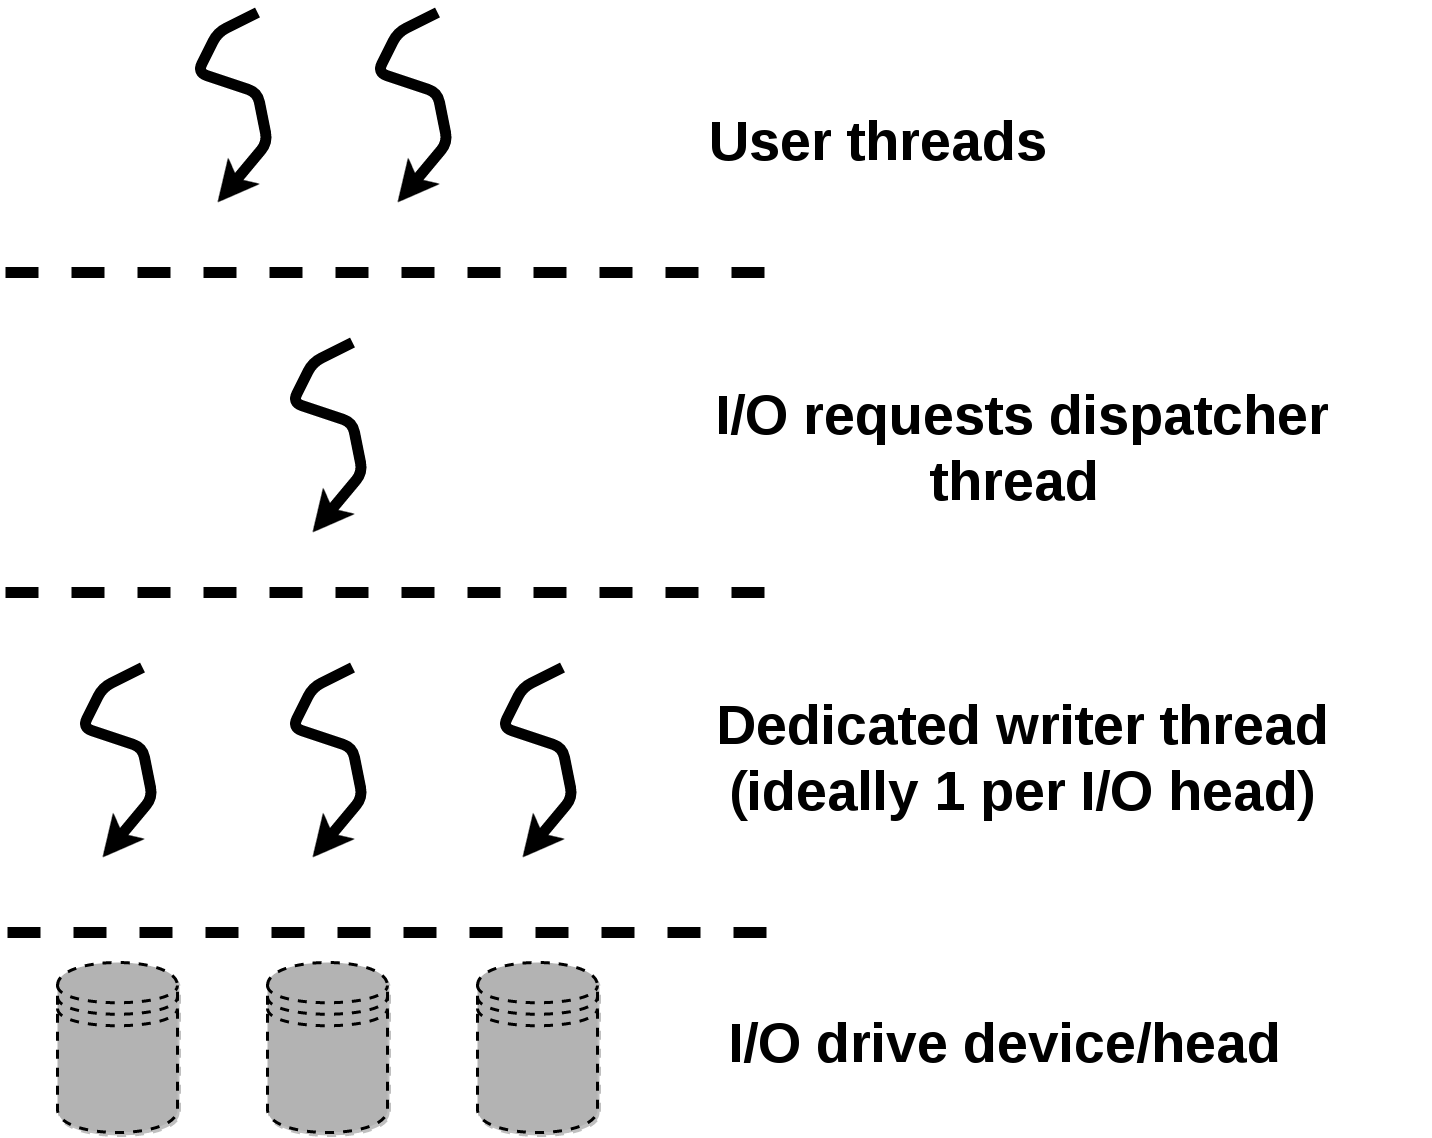
\includegraphics[width=\textwidth]{charts/internship_juelich_posixAIO_basis.png}
				\end{subfigure}
				\caption{POSIX \notationaio\space (\notationaioShort) standard}
				\label{fig:posixAIO_basis}
			\end{figure*}

		Such an approach presents an obvious performance advantage.   The caller thread does not need to wait for the end of the \notationaio\space access.  It might execute other tasks that do not require the end of the resource access.   Given the relatively long time to access the \notationIO\space resource (at processor scale), this might induce a significant reduction of the processor stall time.\\

		Despite these advantages, an intensive usage of the \notationaioShort\space library might be counter-productive in many ways.
		%****** too many writes in parallel *******
		On one hand, the memory footprint of the system may easily sky-rocket, leading to a harmful intensive kernel-swap process (for both user and \notationaioShort\space library threads).   Indeed, each \notationIO\space request may create a potentially large buffer\footnote{The considered buffers are intended to store a memory block which size might be comparable to the live memory (RAM) size.   Hence the explosion of the live memory footprint} which cannot be freed straightforwardly\footnote{In order to allow the user thread to access it asynchronously}.   Given the very small time needed to enqueue an \notationIO\space request, compared to the time to execute it, the user might enqueue a significantly large number of these pending requests.\\

		%******** More threads than IO devices *******
		On the other hand, a miss-calibration of the \notationaioShort\space library\footnote{A calibration that does not suit to the hardware specification.} might lead to a concurrent access to a single \notationIO\space device head, resulting in a dramatic increase of the access time to a given \notationIO\space block.   For instance, let us consider the case where two threads are simultaneously accessing two different blocks\footnote{An \notationIO block is potentially spanning different \notationIO\space sectors} on the same \notationIO\space device (consisting of a single read/write head).   While the head will be scanning a given block, it will be regularly interrupted by requests to scan parts of the other block\footnote{Indeed, scanning a memory block at hardware level is not atomic.   It might have different granularities down to a sector}.   According to Patterson \textit{et al}\cite{patterson1994exposing}, the resulting back-and-forth movement of the \notationIO\space head leads to multiply the access time to a block by up to $10$-fold.\\
		To avoid this hardware interference, all the implementations we present have been tuned to the optimal number of \notationaioWriteThreads: one \notationaioWriteThread\space per \notationIO\space device head.\\

		Our choice of the POSIX \notationaioShort\space library as a foundation of our implementations first aims to limit the engineering effort.   As a matter of fact, the \notationaioShort\space library manages the whole life cycle of all the \notationaioWriteThreads.   It also implements the dispatcher (proxy) thread that receives \notationIO\space requests and forwards them to the \notationaioWriteThreads.   Likewise, the POSIX \notationaioShort\space library might be tuned (number of \notationIO\space devices, number of threads, signal to notify the end of a request process) in order to fit the hardware specifications and the specific \notationIO\space access pattern of the application.\\
		Moreover, the \notationaioShort\space library fits our performance objectives.   Indeed, it efficiently manages, at kernel level, the synchronization of the \notationIO\space resource between the \notationaioWriteThreads.\\
		Considering these services proposed by the \notationaioShort\space library, our engineering effort will focus on the synchronization between the user (caller) thread and the \notationIO\space device-local (\emph{write}) threads.


	\subsection{Synchronizing the \notationaioComputeThread\space and the \notationaioWriteThreads} \label{subsection:synchronization}
		The \notationaioShort\space library manages intrinsically the synchronization between the internal threads that it creates\footnote{Dispatcher and \notationaioWriteThreads}.   It also implements a basic communication mechanism to notify the user about the end of a request's processing\footnote{Effective access to the \notationIO\space resource}.   However, using this mechanism as provided might significantly downgrade the efficiency of the asynchronous strategy within the considered \notationIO\space pattern (see pattern definition in Section \ref{subsection:remapperPattern}).\\
		In this section, we first describe the need we have to implement a synchronization between the user and the \notationaioWriteThreads.   Then, we give an overview of the synchronization mechanism provided by the \notationaioShort\space library.   We explain how it might harm our pattern performances and we describe our solution to enhance it.   Finally, we list the principles that we have followed in our implementations\footnote{Namely the \toolSimulationSoftware\space and the \toolTargetSoftware} to ease and fit this synchronization.\\

		\subsubsection{The need of synchronization}
			%****************** Why we need synchronization (the memory footprint)?
			The main reason why an efficient synchronization mechanism is vital for \notationaio\space is to prevent from memory foot-print explosion.   Indeed, as introduced in Section \ref{subsection:AIO_posix_standard}, the \notationaio\space (and the overlapped accesses to \notationIO\space in general) might lead to a significantly large number of pending requests and of corresponding buffers.   Given the potentially large amount of data carried by these buffers (relative to \notationIO\space disk size), this may easily lead to run out of usable live-memory addresses.   It might also dramatically reduce the overall performances due to the subsequent OS-swap (RAM swap).\\
			By synchronizing the \notationaioComputeThread\space (one that produces the buffers) with the \notationaioWriteThreads\space (those that consume them), the user can expect to access the buffers right after they are processed then remove them.   Hence the reduction of the memory footprint.   However, the important question that remains is: how to make such a synchronization harmless to the performances of the \notationaioComputeThread.   Moreover, how to extend this synchronization in order to regulate the amount of simultaneous buffers before they are created\footnote{This regulation must be triggered on demand: when the memory footprint exceeds a given critical threshold, any creation request should be delayed}.\\

			%****************** Define the AIO synchronization mechanism and its drawback.
			The synchronization mechanism proposed by the \notationaioShort\space library consists in sending a signal (UNIX-kernel signal) to the caller thread after the \notationIO\space request has been effectively processed.   The user thread may decide to execute a custom routine handler to this signal or ignore it.   This mechanism fulfils the synchronization purpose described.   However, two main issues might follow on from its usage.


		\subsubsection{Thread-safety issue of the AIO synchronization}
			The signal handler may compromise the correctness of a critical section between the caller and the \notationaioWriteThreads.   As this signal is received asynchronously, the user (caller thread) cannot decide at which moment to execute the handler.   The handler might thus occur while the caller thread is trying to enqueue a new request to the structure shared with the \notationaioWriteThreads.   As the handler might also require an access to this structure, the single-access principle of this critical section is violated.\\

			%****************** Describe our patch of the nasic AIO synchronization mechanism
			Our solution to avoid thread-safety corruption on the \emph{caller} thread is to forward the execution of the handler to a delegated thread.   This prevents the \emph{caller} execution from being interrupted by any handler.   It also spares the user from implementing a specific critical section to prevent from the handler's execution at inappropriate moments.   


		\subsubsection{Time overhead on the \notationaioComputeThread}
			Executing the handler corresponding to the \notationaio\space signal might create a significant time overhead on the caller (\emph{compute}) thread.   As a mater of fact, this handler interrupts the execution of the caller thread in order to process its own code.   Even more damaging, this handler might require a significant time to process.   It might, for instance, require to access its corresponding buffer\footnote{Buffer which execution has triggered the current handler} (in order to remove it or to check the correct execution of the \notationaio\space request).   Given that this buffer has been processed by another thread (\notationaioWriteThread), its access requires to import it from a potentially distant cache on a potentially distant \emph{NUMA} socket and invalidate it.   Considering the size of such a buffer, this remote \emph{NUMA} node importation is very likely to create false-sharing (see Section \ref{subsection:lightenFalseSharing}).   Hence, the increase of the response time of both the current thread (\emph{caller}) and the one running on the remote \emph{NUMA} node (\emph{writer}).\\

			%****************** Describe our patch of the nasic AIO synchronization mechanism
			Our solution to avoid time overhead on the \emph{caller} thread is the same as that addresses the thread-safety issue.   It consists in forwarding the execution of the handler to a delegated thread.   This allows the \emph{caller} thread to have no delay due to the handler\footnote{Assuming a sufficient number of CPU-cores}.   It also spares the user from implementing a specific critical section to prevent from the handler's execution at inappropriate moments.   Ideally, this delegated thread would be the \notationaioWriteThread\space that has just processed the corresponding request (for core and cache proximity reasons).


		\subsubsection{Improving the \notationaioShort\space synchronization}\label{subsubsection:pthreadWrapper}
			In our implementations, applying any modification to the thread creation and management is not straightforward.   Indeed, these threads are created by the POSIX \notationaio\space library; a UNIX standard library with no certified open-source version available.   Thus, it was not possible to change the thread creation part of this library nor to re-assign the workload between threads.\\
			Our solution was then to wrap up the so-called \emph{pthread} library.\\

			Our solution is to make the thread-creation-request (and few other thread-management-requests) called by the standard \notationaio\space library to be forwarded to our custom wrapper of the \emph{pthread} library.   Our wrapper manages the thread creation and affinity with unique CPU-cores\footnote{The specification and the deployment process of the custom thread library have been released in \href{https://github.com/simbadSid/cubeRemapper\_perfBenchmark}{https://github.com/simbadSid/cubeRemapper\_perfBenchmark}}.   It also allows to attribute custom functionalities to some specific threads.\\

			This solution has led us to build a custom implementation of the \toolTargetSoftware\space referred to as the \emph{\notationaio-pinned thread} version.\\

			Despite the interest of this custom wrapper library, this solution has not been shipped to our final version of the \toolTargetSoftware.   Indeed, wrapping the standard \emph{pthread} library with our custom one requires a non-negligible human intervention before running the \toolTargetSoftware\footnote{For instance, the user would need to set the \emph{LD\_PRELOAD} environment variable with our custom library.   And an unexpected exit of our software would make our custom library be called by default by any other application}.   Such a requirement would make the \toolTargetSoftware\space less user-friendly.   Therefore, unless otherwise specified, our custom wrapper library will not be used in the experiments which will be presented in the next chapter.


	\subsection{Data distribution among threads}\label{subsection:dataDistribution}
		\subsubsection{Custom shared data structure}\label{subsubsection:customDatastructure}
			%****************** Reduced number of shared data and instructions between threads (separated buffer not reused by compute + synchronized queue that allows an optimized access to the only shared structure)
			The two previous solutions aim to enhance the synchronization between the \notationaioComputeThread\space and the \notationaioWriteThread.   The efficiency of such solutions relies on an adequate thread-proximity of the data.   The pattern that we consider is, by design, adapted to such a data distribution (see section \ref{subsection:remapperPattern}).   Our engineering effort has thus focused on the data structure used for the synchronization of the \notationaio\space requests (see Figure \ref{fig:synchronization}).   Our structure implements all the used blocking operations through the \emph{enqueue} and \emph{dequeue} operations.   It also enhances thread proximity by using separate ends for the \emph{enqueue} (\notationaioComputeThread) and \emph{dequeue} (\emph{write} or \emph{handler} thread).\\

				\begin{figure*}[!h]
					\centering
					\begin{subfigure}[b]{0.65\textwidth}
						\centering
						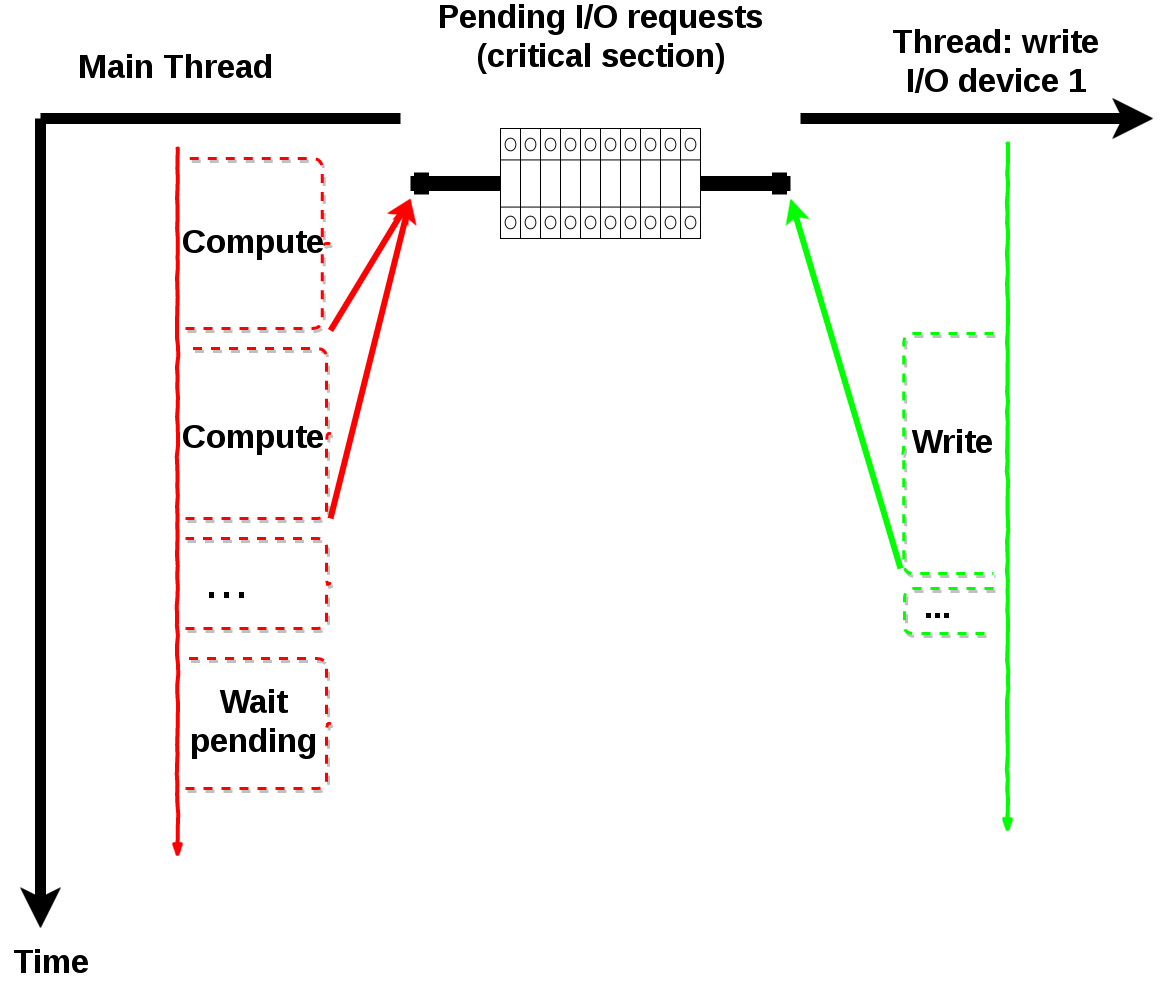
\includegraphics[width=\textwidth]{charts/internshipJulich_AIO-synchronization.png}
					\end{subfigure}
					\caption{Synchronization scheme of the \notationaioComputeThread\space with the \notationaioShort\space threads}
					\label{fig:synchronization}
				\end{figure*}

		\subsubsection{Reducing the impact of \emph{false-sharing}}\label{subsubsection:lightenFalseSharing_concept}
			Among the factors that can limit the efficiency of concurrent algorithms, the shared memory is probably the one that has the deepest impact.   In section \ref{subsubsection:synchronization} we have presented our try to reduce the number of shared memory addresses (at RAM level) and lighten the impact of synchronization between threads.   Let us now reduce even more this shared data impact at cache level.   Our purpose is to address the well-known issue of \emph{false-sharing}.\\

			Let us consider two independent memory buffers used by two concurrent threads.   For clarity, let us also consider that each thread is running on an independent core.   Although the two buffers share no common address, they might still be stored by the same cache line (see Figure \ref{fig:falseSharing_concecpt}).   As the granularity of a cache is a line, then modifying one buffer will lead to the invalidation of the other one.   Likewise, accessing the unmodified buffer will require to import the content of the remote cache line.   Thus a significant overhead at each \emph{read} and \emph{write} access.   This drawback of multithreaded applications is known as \textbf{\textit{false-sharing}}.\\
			Knowing that in our implementation all the concurrent threads (\emph{compute} and \emph{write} operations) are processing \emph{write} accesses, we can easily imagine the high frequency of this costly and idle back-and-forth cache routine.   An assessment of this cost will presented in next chapter (Section \ref{subsection:lightenFalseSharing}).\\

				\begin{figure*}[!h]
					\centering
					\begin{subfigure}[b]{0.55\textwidth}
						\centering
						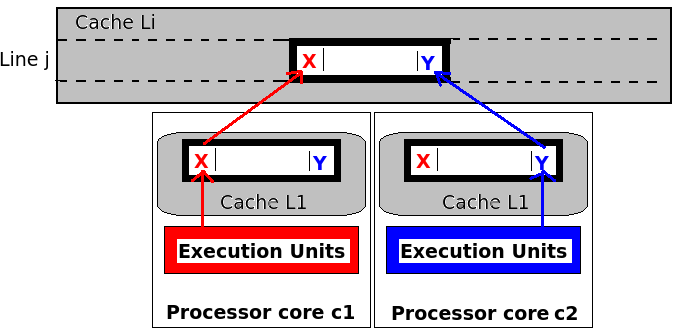
\includegraphics[width=\textwidth]{charts/falseSharing_concecpt.png}
					\end{subfigure}
					\caption{\emph{False-sharing} concept}
					\label{fig:falseSharing_concecpt}
				\end{figure*}

			Our solution to avoid \emph{false-sharing} between concurrent threads is to align each buffer accessed by the concurrent threads to a cache line.   By doing so, we ensure that each buffer is stored within an independent cache line.   Thus, each access to this buffer will be done independently from any other thread.\\

			This solution has led us to build a custom implementation of the \toolTargetSoftware\space referred to as the \emph{\notationaio-buffer aligned} version.

%			Tackling the impact of \emph{false-sharing} on our version of the \toolTargetSoftware\space lead us to a custom implementation referred to as \emph{\notationaio-buffer aligned}.   An evaluation of this version and its improvement is proposed in the next chapter (see Section \ref{subsection:lightenFalseSharing}).

		\subsubsection{Custom dynamic memory allocation}\label{subsubsection:customDynamicMemoryAllocation_concept}
			Let us now see how to go further in limiting the contention on shared data at cache level (primarily L3).   Our objective is to smooth the interaction between the \emph{compute} and the \notationaioWriteThreads.\\
			Our main purpose here is to tackle the dynamic-memory-allocation drawback.   The objective being to make the dynamic memory allocation (invoked at each \emph{compute} operation) less time-consuming and better fit the specification of the allocation-pattern of our application.\\
			To do so, we describe in this section two solutions to undermine the impact of two main performance bottlenecks (relative to multithreading) of a general-purpose memory allocators\footnote{Such as the Linux-standard glibC library: ptmalloc\cite{robertson2003run}}.   Applying this approach on the \toolTargetSoftware\space has led us to implement a custom dynamic memory allocator.\\

			We should mention that our memory allocator has, by design, a significant advantage on the general-purpose allocators (in addition to the three key points described bellow).   Indeed, our allocator is based on a user-level-managed heap chunk.   Thus, the \emph{allocation} and \emph{free} operations require no system calls (unlike the general-purpose allocators).   The inherent advantage of this design choice is not discussed neither assessed in this report.\\

			%***************Take advantage of the specificity of our memory allocation pattern: addresses aligned to ...   Thus we can manage the dynamic memory as a bunch of fixed-size blocks.   Hence no external nor internal fragmentation of the free memory\\
			The first design of our custom memory allocator is to take advantage of the specificity of our memory allocation pattern.   This is done through managing the free memory as fixed-size blocks (unique size equal to a cache line).   Indeed, each allocation needs to be aligned to a given address (see Section \ref{subsubsection:lightenFalseSharing_concept}).  Thus, it is useless to split such a memory block during the allocation: the extra memory (till the next alignment address) will never be required.\\
			Consequently, our dynamic memory management is simplified and reduced to pointer arithmetic.   This considerably reduces the management time and memory footprint.\\
			Our custom allocator has no external fragmentation to deal with.   Meanwhile, the effect of the created internal fragmentation is lightened by the OS: as the extra addresses are not know by the user, they will most likely never be used.   Thus, the OS will swap them out\footnote{As a memory blocks has a cache-line size, it will be swapped out into single page.   It will also create no residual in the RAM}, which will almost completely remove any time and memory space impact.\\

	%		***************Improve the synchronization between allocation (compute) and free (write) which might be made by independent threads\\
			The second design we came with is to store our free memory blocks within a structure with two independent ends:  one to allocate a block and the other to return a freed block (see Figure \ref{fig:customMemAlloc_freePool}).   Indeed, when couple with our \notationaio\space strategy, this structure ensures that the thread that allocates memory (the compute thread) is not the one that frees it (after the write thread work).   Thus, our distributed architecture allows to soften the contention on the shared free memory structure.  As the \emph{free} operation may be processed in parallel, we have designed the \emph{free} end of the shared memory structure as a "Treiber" stack \cite{pedersen1998method}:   a lock free stack that ensures thread-safety using the hardware atomic primitive: \emph{compare-and-swap}\cite{valois1995lock}.   This ensures a thread-safety to this structure without any software synchronization.\\
				\begin{figure*}[!h]
					\centering
					\begin{subfigure}[b]{0.7\textwidth}
						\centering
						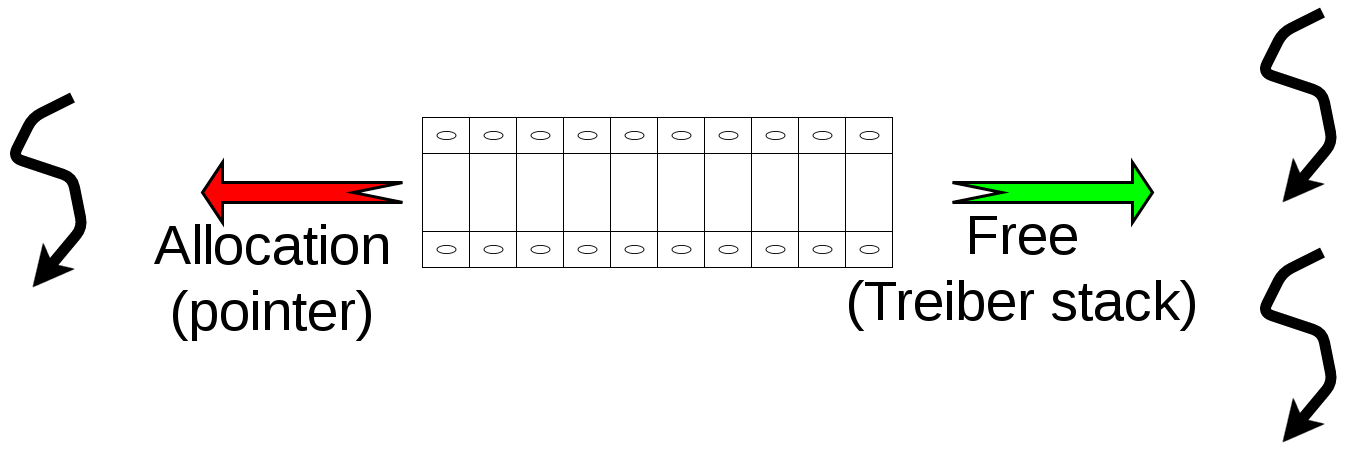
\includegraphics[width=\textwidth]{charts/internship_juelich_customMemAlloc_freePool.png}
					\end{subfigure}
					\caption{Free dynamic memory architecture}
					\label{fig:customMemAlloc_freePool}
				\end{figure*}

			The incorporation of this custom memory allocator has led us to build a custom implementation of the \toolTargetSoftware\space referred to as the \emph{\notationaio-full-fledged} version.


	\subsection{The \toolTargetSoftware\space custom implementation (asynchronous)} \label{subsection:remapperPattern}
		%****************** The main objective of the whole work: optimize the response time of this software
		As described in Section \ref{section:cubeRemapper_stateOfTheArt}, the execution time of the \toolTargetSoftware\space has a significant portion of processor idle time.   Indeed, at each iteration of this software, the \emph{compute} operation is followed by a \emph{write} operation.   Due to the important amount of data stored on the hard disk, this operation has a significant impact on the overall execution time.\\
		Our objective is to reduce the stall time of the processor by overlapping the \emph{compute} with the cause of the processor stall: the \notationIO\space \emph{write} function.   The \notationaioShort\space library and the custom synchronization method that we have previously described are the foundations of the improvement we want to bring to the \toolTargetSoftware.\\

		\begin{figure*}[!h]
				\centering
				\begin{subfigure}[b]{0.33\textwidth}
					\centering
					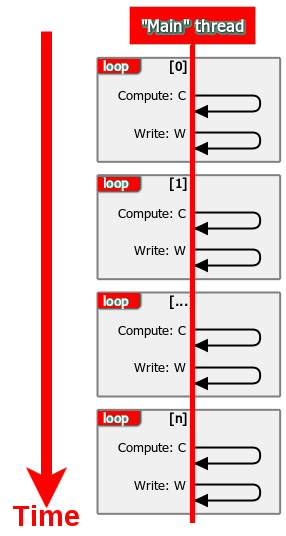
\includegraphics[width=\textwidth]{charts/internshipJulich_model_0-IO-simple.png}
					\caption[Synchronous case]
					{{\small Synchronous case}}
				\end{subfigure}
				\hfill
				\begin{subfigure}[b]{0.475\textwidth}  
					\centering
					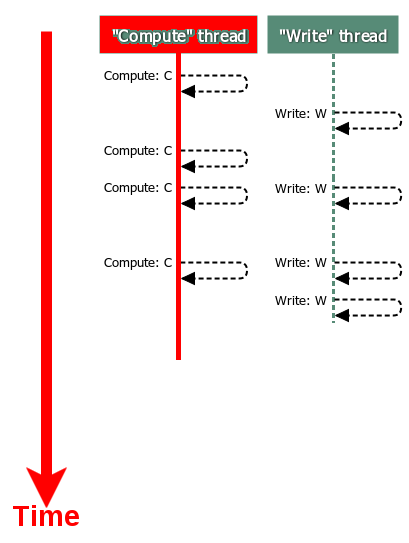
\includegraphics[width=\textwidth]{charts/internshipJulich_model_0-AIO-simple.png}
					\caption[]%
					{{\small Asynchronous case}}
				\end{subfigure}
				\caption{\notationAIO\space applied to the \toolTargetSoftware\space pattern}
				\label{fig:AIO_basis}
			\end{figure*}

		%****************** Describe the simulation test-bed implementation
		The main idea behind our implementation of the \toolTargetSoftware\space is summarized in Figure \ref{fig:AIO_basis}.   Let us consider the main loop of the \toolTargetSoftware.   Thanks to the \notationaioShort\space library, we expect to overlap the execution of each \emph{write} operation with one of the next computations.\\
		For such a strategy to succeed, one must ensure that the two operations (\emph{compute} and \emph{write}) are using totally independent memory addresses (except the one used for the synchronization).

	\subsection{The \toolSimulationSoftware} \label{subsection:simulationTestbed}
		In order to assess the solution we propose for the \toolTargetSoftware, one could simply ship it to the \toolTargetSoftware\space and evaluate its performances.   However, the \emph{compute} operation of the \toolTargetSoftware\space involves different and highly-random memory access patterns (at RAM level).   It also allocates and deals with significantly large chunks of the process stack.   Thus, it might have unexpected impacts on the \emph{write} operation that we implement.   It might also have a performance impact on the synchronization between the \notationaioComputeThread\space and the \notationaioWriteThreads.   Finally, it might be extremely sensitive to remote memory-accesses on the data it generates\footnote{The interferences (between concurrent threads) that we consider here take place mainly at cache level.   At RAM level, such an interaction is harmless due to the synchronization we have designed}.   In Section \ref{section:experimentalCase}, we will present an experimental assessment of this potential interferences and we will show the huge impact that they might have on our implementation of the \toolTargetSoftware\space (basic version).\\

		To avoid dealing with these interferences (in a preamble step), we have decided to simplify the global pattern of the \toolTargetSoftware\space through a custom and independent program (\toolSimulationSoftware).   This \toolSimulationSoftware\space allows to reduce the response time of the system down to the two operations: \emph{compute} and \emph{write}.   It also gets ride of the numerous potential sources of perturbation by simplifying these two operations.   It is used as a preliminary test for our theoretical models.\\
		At the same time, our simulator may use different strategies to simulate the complex \emph{compute} operation of the \toolTargetSoftware.   This allows to observe different behaviours of the \toolTargetSoftware\space without having to find the inputs that would trigger such a behaviour.   One may, for instance, observe different \emph{compute} times or live-memory access patterns.   From a purely theoretical perspective, our \toolSimulationSoftware\space allows to assess different aspects of the \toolTargetSoftware\space pattern within different domains.   This intends to confirm the potential performance gain of our solution.   It would also help us identify the domain where such a gain would be optimal.\\

		The main principle behind the \toolSimulationSoftware\space is described on the listing \ref{code:simulator}.   The algorithm used for the \emph{compute} and the \emph{write} operations are set through the usage of different implementations of the same "Worker" interface.\\
		\begin{minipage}{\linewidth}
			\begin{lstlisting}[language=C++, caption={\toolTargetSoftware\space \toolSimulationSoftware}, label={code:simulator}]
int main(int argc, char **argv)
{
    unsigned int nbIteration, computeTime, bufferSize, nbIoDevice, nbProc;

    extractParameter(argc, argv, &nbIteration,
                     &computeTime, &bufferSize, &nbIoDevice,
                     &nbProc, &memAccessPattern);
    // Pick the implementation to use for the "compute"
    // and the "write" operations
    Worker worker = Worker.generate(nbIteration, computeTime, bufferSize,
                                    nbIoDevice, nbProc);

    for (int i=0; i<nbiteration; ++i)
    {
        char *buffer = worker.compute();
        worker.write(buffer);
    }

    worker.waitPendingRequest();

    return 0;
}
			\end{lstlisting}
			\end{minipage}
		This code also shows the main parameters of the simulation that might be tuned:
		\begin{itemize}
			\item Number of iterations
			\item Compute time (per iteration)
			\item Number of hardware \notationIO\space devices (used to determine the number of concurrent \notationaioWriteThreads)
			\item Number of concurrent CPU-cores (used to initialize the \notationaioShort\space library internal thread synchronization)
			\item Buffer size used at each computation
		\end{itemize}


%--------------------------------------------
\section{Proposed theoretical models}\label{section:model}
	In this section, we propose two theoretical models for the response-time of our custom (\notationaio) implementations.   We also try to enhance these models in order to fit the HPC platform specifications (multiple parallel \notationIO\space devices and reduced computation time).\\
	These models are used to determine the parameters\footnote{Example: \emph{compute} time, \emph{write} buffer size} that influence most our solution.     They will also help us (in Section \ref{subsection:AIO_firstApproachAssessment}) to confirm the potential gain brought by our solution (from a theoretical perspective).   Finally, they will help us determine the domain where our solution may bring a significant improvement.\\

	Clearly, the gain brought by our proposed algorithm will be compared to the existing synchronous model given by the following Equation (\ref{equation:synchronousModel}):
	\begin{equation}
	\begin{aligned}
		T_{synchronous}	= n * (C + W)
		\label{equation:synchronousModel}
	\end{aligned}
	\end{equation}
	In this model, all the instructions are serialized.   Thus, the total execution time is simply the sum of all the execution times.\\

	To conduct our experimentations, we assume that the size of the buffer written at each iteration is constant (for a given experimentation).   We also assume that the computation time $C$ at each iteration is constant (for a given experimentation).\\
	The following notations are used to express the theoretical model of our asynchronous version of the \toolTargetSoftware:
	\begin{itemize}
		\item $C$: computation time at each iteration
		\item $W$: size of the buffer written at each iteration
		\item $n$: number of iterations
		\item $P$: number of computation-cores available
		\item $N_{io}$: number of independent \notationIO\space access heads (only used in section \ref{subsection:multipleParallelIoDevice})\\
	\end{itemize}


	\subsection{First approach: simple write/compute representation (single \notationIO\space device)} \label{subsection:firstModel}
		In this first approach, we present a simple model by introducing the following hypotheses:
		\begin{itemize}
			\item Constant writing time $W$ of each buffer.
			\item Perfect parallelization model (execution time with $p$ computation cores $T(p) = \frac{T(1)}{p}$).
		\end{itemize}
		Thus, the execution time of the asynchronous pattern would be:
			\begin{equation}
			\begin{aligned}
				T_{asynchronous}&= C + W + (n-1) * max(C , W)
			\end{aligned}
			\label{equation:model0}
			\end{equation}
		Indeed, the first computation time and the last writing time (the two first terms of the above equation) cannot be avoided or softened.   Then, the \emph{compute} and the \emph{write} operations are executed by two independent threads (ideally with no interference between them).   Hence, we only retain the maximum execution time of the two threads: $max((n-1)*C, (n-1)*W) = (n-1) * max(C, W)$.\\

		In this model and for the seek of simplicity, we deliberately get ride of the scheduling and pseudo-parallelization\footnote{Pseudo-parallelization happens when 2 concurrent threads are executed on the same mono-threaded core} overhead.   This decision is also motivated by the limited impact of these phenomena regarding the range of the considered writing and computing times (see the \emph{write} time evaluation in Section \ref{subsection:AIO_firstApproachAssessment}).\\

		By analysing the asymptotic behaviour of Equation (\ref{equation:model0}), one may use the following approximations:
			\begin{equation}
			\begin{aligned}
				T_{asynchronous}	\stackrel{\text{if C << W}}{\approx} n * W + C
									\stackrel{}{\approx} n * W
			\end{aligned}
			\label{equation:model0:C<<W}
			\end{equation}
			\begin{equation}
			\begin{aligned}
				T_{asynchronous}	\stackrel{\text{if C >> W}}{\approx} n * C + W
									\stackrel{}{\approx} n * C
			\end{aligned}
			\label{equation:model0:C>>W}
			\end{equation}


	\subsection{Second approach: modelling the perturbations (single \notationIO\space device)} \label{subsection:secondModel}
		The previously-generated model allows a simple estimation of our version of the \toolTargetSoftware\space pattern.   However, it relies on hypotheses that make it hardly scalable.
		While trying to enhance this model, we have experimentally observed (see Section \ref{subsection:AIO_firstApproachAssessment}) that the difference between the theoretical model and its experimental evaluations seems constant (with respect to the computation time).   Based on this finding, we propose the following improved second model:
			\begin{equation}
			\begin{aligned}
				T_{asynchronous}&= C + W_{perturbation} + (n-1) * max(C , W_{perturbation}) + n * req
			\end{aligned}
			\label{equation:model1}
			\end{equation}
		Where:
		\begin{itemize}
			\item $req$ is the time to transmit the \emph{write} request (or enqueue it for later execution).
			\item $W_{perturbation}$ is the delay of the \emph{write} operation introduced by the payload and the contention on the \notationIO\space device.
		\end{itemize}
		In this second model, we try to express the previously-observed perturbations\footnote{Gap between the theoretical model and the experimental evaluation} by introducing the two expressions $req$ and $W_{perturbation}$.   These two expressions do not depend on the computation time; hence, each one of them can potentially explain the constancy of the observed perturbation.\\

		\subsubsection{Modelling the writing time ($W_{perturbation}$)}\label{subsubsection:modelWritingTime}
			% Context
			When we estimate the overall time response of the \toolTargetSoftware\space pattern, the experimental errors of the \emph{write} time at each iteration are summed up.   This may eventually have a significant impact on the total response time.  In this section, we no longer consider the \emph{write} time as constant and try to fit more accurately its variations.\\

			% Identify the pb: write time is not constant
			Providing an accurate measurement of the \emph{write} time maybe very complex (even when we consider buffers with constant sizes).   The \emph{write} time may highly vary depending on the processor family\footnote{Here we mainly refer to the number of cores and physical threads.}, the previously processed \notationIO\space requests, the detected \notationIO\space access pattern\cite{petrovic2015performance}, or even some unexpected external parameters (such as the system temperature or some magnetic interferences)\cite{lu2003performance}.
			% Reason why we initially did this hypothesis
			However, we still need to estimate it to validate our theoretical model.\\
			% Our solution

			Our solution to overcome this difficulty is to consider the writing time as constant but only at saturation regime.   This solution is inspired from the "I/O saturation method" introduced by R. Robert \emph{et al}\cite{ross2001case}.   It consists in measuring the time to write a given buffer after flooding the \notationIO\space system with concurrent \emph{write} access (following a given access pattern).   In order to measure the required \notationIO-saturation level\footnote{Depends on the hardware \notationIO\space specification} and apply the \notationIO-saturation during the write-time measurement, we have used the code released by the above-cited reference.\\

		\subsubsection{Modelling the \notationaio\space request time ($req$)}\label{subsubsection:modelRequestTime}
			Let us consider an \notationaio\space request submitted by the \emph{compute} thread.   Such requests are always processed by the main thread in the considered approach.   Thus, their time foot-print cannot be avoided neither divided upon processor cores or \notationIO\space devices.\\
			Within the scope of our study, we consider the \notationaio\space request-time as constant (for a given hardware platform).   Indeed, submitting an \notationaio\space corresponds to simply forward the request-address from the \emph{compute} thread to the \emph{write} thread.   No other computation nor data transfer is performed at this step\footnote{The buffer to be written might be imported by the writer thread later-on when the effective \notationIO\space operation will be processed}.\\

			Our method to evaluate the \notationaio\space request-time\footnote{For a given hardware platforms} is similar to the \notationIO\space write-time evaluation (see Section \ref{subsubsection:modelWritingTime}).   It consists in assessing the time $T$ to submit an \notationaio\space request for different number $n$ of iterations (number of requests submitted): $T = req * n$.   Then, determining $req$ is equivalent to determining the linear model that fits the best the assessed values $(T, req)$.\\

			Thanks to the generated linear-model, we can determine the value of the request time as the slope of the linear model.   We may also confirm our hypothesis (constant \notationaio\space request-time) using the constant term\footnote{Other methods could be applied in order to assess the validity of the linear model (example: the "coefficient of determination" $R^{2}$).   But these would require a benchmark evaluation of the acceptable error}.\\


	\subsection{Introducing multiple parallel \notationIO\space devices} \label{subsection:multipleParallelIoDevice}
		In this section, we suppose that the hardware platform has at its disposal $N_{io}$ independent \notationIO\space devices.   Hence, at most, $N_{io}$ independent \notationIO\space operations maybe performed concurrently.   For simplicity, we assume in this section that the parallel \notationIO\space model is perfect: two concurrent \notationIO\space operations on two different \notationIO\space devices will not create any interference on each others.   We also assume that the number $N_{io}$ of \notationIO\space devices is much smaller than the number $n$ of iterations (for the simplicity of the model expression).\\

		Thanks to Equation (\ref{equation:model0:C>>W}), we can notice that when $C >> W$, the time response of our system does not depend on the writing time $W$\footnote{However $W$ appears in this equation, it is a simple added element with no coefficient.   Thus this write time $W$ can not be split over multiple devices.}.   Thus, introducing additional parallel \notationIO\space devices will not affect this response time (see Figure \ref{subFig:model0_multipleIoDevice_C>>W}).   Hence, our model in this case remains:
			\begin{equation}
			\begin{aligned}
				T_{asynchronous}(N_{io})	\stackrel{\text{if C >> W}}{\approx} n * C + W
											\stackrel{}{\approx} n * C
			\end{aligned}
			\end{equation}
		By simply extending this model to the case where $C \approx W$, we can see (Figure \ref{subFig:model0_multipleIoDevice_C=W}) that additional \notationIO\space devices are still useless.   The model in this case remains:\\
			\begin{equation}
			\begin{aligned}
				T_{asynchronous}(N_{io})	\stackrel{\text{if C = W}}{\approx} n * C + W
											\stackrel{}{\approx} n * C
			\end{aligned}
			\end{equation}
			\begin{figure*}[!h]
				\centering
				\begin{subfigure}[b]{0.475\textwidth}
					\centering
					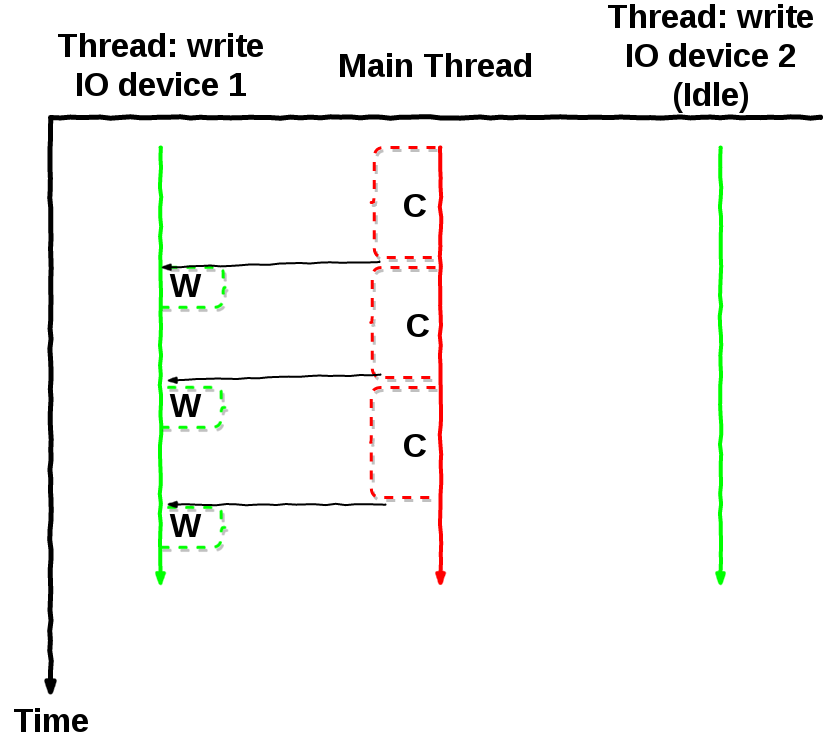
\includegraphics[width=\textwidth]{charts/internshipJulich_AIO-multipleIoDevice_CBiggerThanW.png}
					\caption[Computation time $>>$ Write time]%
					{{\small Computation time $>>$ Write time}}
					\label{subFig:model0_multipleIoDevice_C>>W}
				\end{subfigure}
				\hfill
				\begin{subfigure}[b]{0.475\textwidth}  
					\centering 
					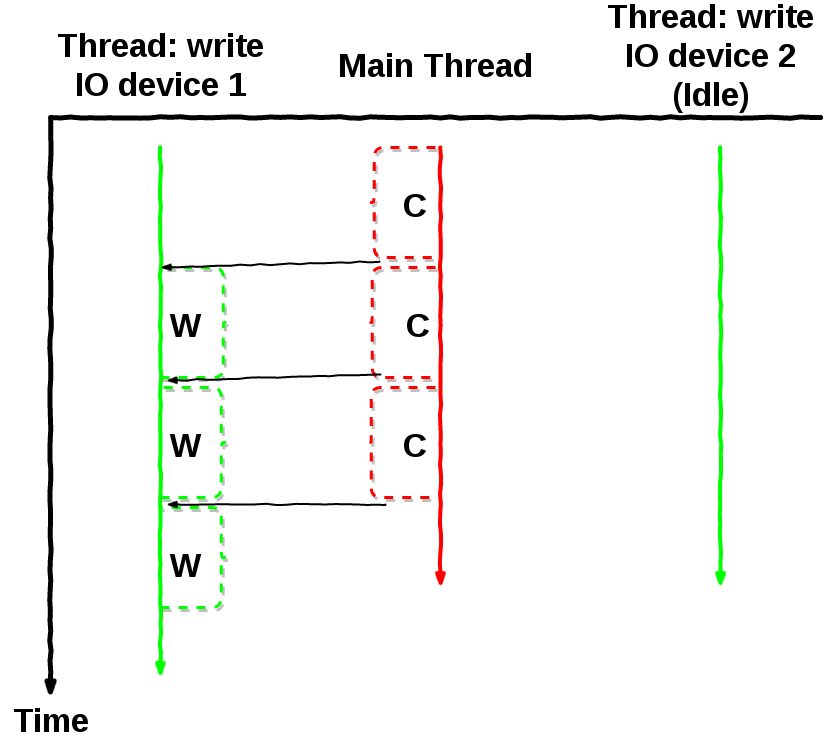
\includegraphics[width=\textwidth]{charts/internshipJulich_AIO-multipleIoDevice_CEquivalentToW.png}
					\caption[]%
					{{Computation time $\approx$ Write time}}
					\label{subFig:model0_multipleIoDevice_C=W}
				\end{subfigure}
				\vskip\baselineskip
				\begin{subfigure}[b]{0.475\textwidth}
					\centering
					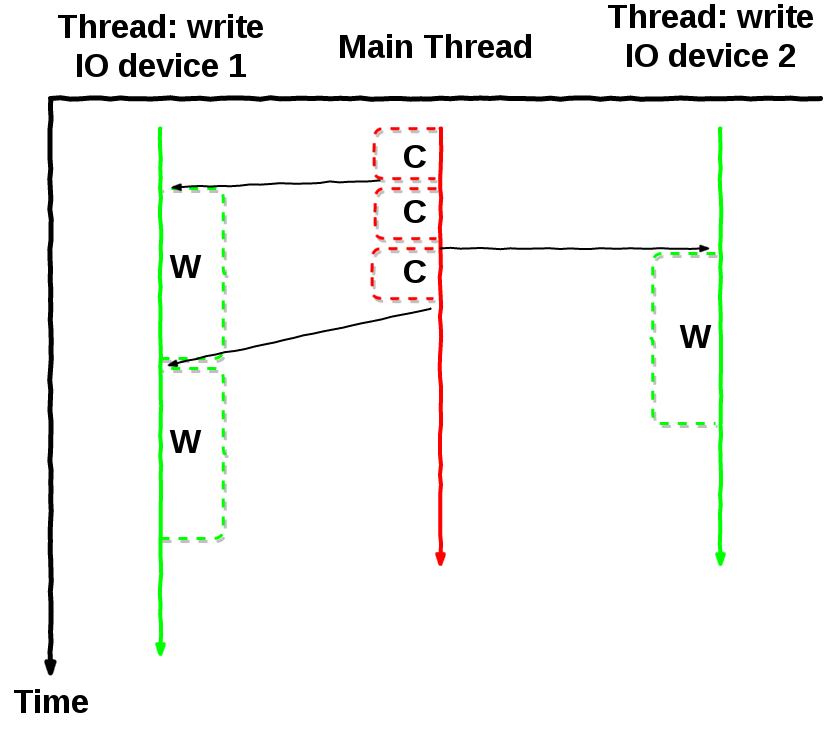
\includegraphics[width=\textwidth]{charts/internshipJulich_AIO-multipleIoDevice_CSmallerThanW.png}
					\caption[]%
					{{\small Computation time $<<$ Write time}}
					\label{subFig:model0_multipleIoDevice_C<<W}
				\end{subfigure}
				\caption[Asynchronous \notationIO\space pattern diagram with multiple \notationIO\space devices]
				{\small Asynchronous \notationIO\space pattern diagram with multiple \notationIO\space devices}
				\label{fig:model0_multipleIoDevice}
			\end{figure*}
		Finally, in the case where $C << W$, the number of \notationIO\space devices becomes relevant (see Figure \ref{subFig:model0_multipleIoDevice_C<<W}).   The new inflection point (computation time where this model becomes applicable) is $C = \frac{W}{i}$.   The theoretical model in this case becomes:\\
			\begin{equation}
			\begin{aligned}
				T_{asynchronous}(N_{io})	& \stackrel{\text{if C << W}}{\approx} (n-1) * max(\frac{W}{N_{io}}, C) + C + W			\\
				T_{asynchronous}(N_{io})	& \stackrel{\text{if C << }\frac{W}{N_{io}} }{\approx} (n-1) * \frac{W}{N_{io}} + C + W		\\
				T_{asynchronous}(N_{io})	& \stackrel{\text{if C } \in [\frac{W}{N_{io}}, W] }{\approx} (n-1) * C + C + W
											\stackrel{}{\approx} n * C + W
			\end{aligned}
			\label{equation:model0_multipleIoDevice_C<<W}
			\end{equation}


%--------------------------------------------
\section{Target hardware platform and compatibility}
	\subsection{Hardware platform}
		%******************  Need to a highly multithreaded (physical thread) machine:
		The performance profiling and measurement tools that we are developing are intrinsically designed for highly-multithreaded (physical thread) hardware platforms.   There principle purpose is to track and profile performance-bottlenecks that are due to the contention of concurrent (threads or processes) execution.   These tools aim to assess each unitary\footnote{Thread, process or job execution} execution.   They also aim to evaluate the communication and the interaction between these executions\footnote{\emph{MPI} or kernel-level (ex: pipe, socket) communication}.   These dimensions can only be set and observed on a hardware platform that physically\footnote{In this study we do not consider virtual hardware environments.} allows an execution at such concurrent scale.\\

		%****************** Why HPC platform?
		As we consider highly-concurrent hardware platforms, HPC platforms are obvious candidates.   For the experimental assessment of our study, we made such a choice (see section \ref{section:experimentalSetup})  for both practical and functional intends.\\

		On one hand, our study has been conducted within an environment of cutting-edge HPC-specific performance track researches.   Our goal to outperform the \toolTargetSoftware \cite{saviankou2015cube} is part of a global project\footnote{Scalasca project\cite{zhukov2013assessing}} that aims to develop a set of tools that provide highly scalable performance measurement and analysis for computation at HPC scale.   Our work is thus part of a framework to enhance and automate the profiling of parallel and distributed applications at HPC scale.\\

		On the other hand, an HPC platform represents an ideal experimental set-up for our theoretical study about overlapped \notationIO-accesses.   The HPC platforms we considered (see Section \ref{section:experimentalSetup}) has at its disposal several parallel and independent \notationIO\space devices, managed by a shared file system.   Moreover, as mentioned in Section \ref{subsection:AIO_posix_standard}, the number of concurrent \notationaioWriteThreads\space is limited by the number of independent \notationIO\space devices.   Hence, thanks to the HPC's numerous independent \notationIO\space devices, one could expect that the \notationaio would bring a significant additional gain.\\

		Thanks to the specification of the considered HPC hardware (see Section \ref{section:experimentalSetup}), the overlapping and the parallelization implemented by our solution maybe reached with a reduced time overhead.   In this context, the high number of CPU-cores and the large cache size are two commonly-considered helping factors.   However, the \emph{Hyper-Threading} technology\cite{magro2002hyper}\footnote{The \emph{Hyper-Threading} technology is not specific to the HPC platforms.   It is an \emph{Intel} technology that is also deployed on some modern Intel servers} is probably the most influencing design of such a hardware architecture on our approach.\\
		The \emph{Hyper-Threading} technology allows two threads to run concurrently on the same CPU-core:   there relative micro-instructions (except the load/store instructions) being processed in parallel as if they where running on two distinct CPU-cores.   As shown in Figure \ref{fig:hyperThreading}, the advantage of such a design, compared to physical parallelization\footnote{Two concurrent threads running on two independent CPU-cores}, comes from the optimal cache proximity of the shared data at all cache levels (L1, L2, L3 (data and instruction) and \emph{Translation Lookaside Buffer}).\\
		In the ideal case, this would allow the \notationaioComputeThread\space (producing the buffers) and the \notationaioWriteThread\space (consuming the same buffers) to run simultaneously on the same CPU-core.   By doing so, we take advantage of the parallelization\footnote{Unlike pseudo parallelization where two concurrent threads run on the \emph{same CPU-core} by interrupting each others}.  Additionally, the shared buffer will not need to be moved from the producer core to the consumer core.   Hence the optimal cache proximity.\\
		The same cache proximity advantage can be noticed on the \emph{Translation Lookaside Buffer} (TLB).   The address translation\footnote{Virtual-physical and physical-virtual address translation} used by the \notationaioComputeThread\space is similar to the one used by the \notationaioWriteThread\space (in the specific execution case described earlier).   Thus, the content of the TLB might be reused by the \notationaioWriteThread\space without cache-misses.\\

			\begin{figure*}[!h]
				\centering
				\begin{subfigure}[b]{0.48\textwidth}
					\centering
					\frame{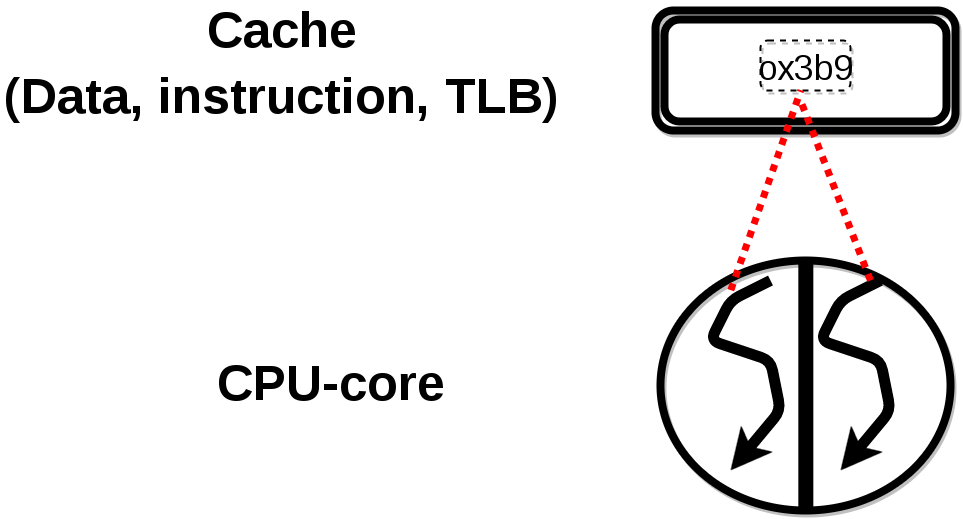
\includegraphics[width=\textwidth]{charts/internshipJulich_hyperthreading.png}}
					\caption[Hyper-Threaded core]
					{{\small Hyper-Threaded core}}
				\end{subfigure}
				\hfill
				\begin{subfigure}[b]{0.48\textwidth}  
					\centering
					\frame{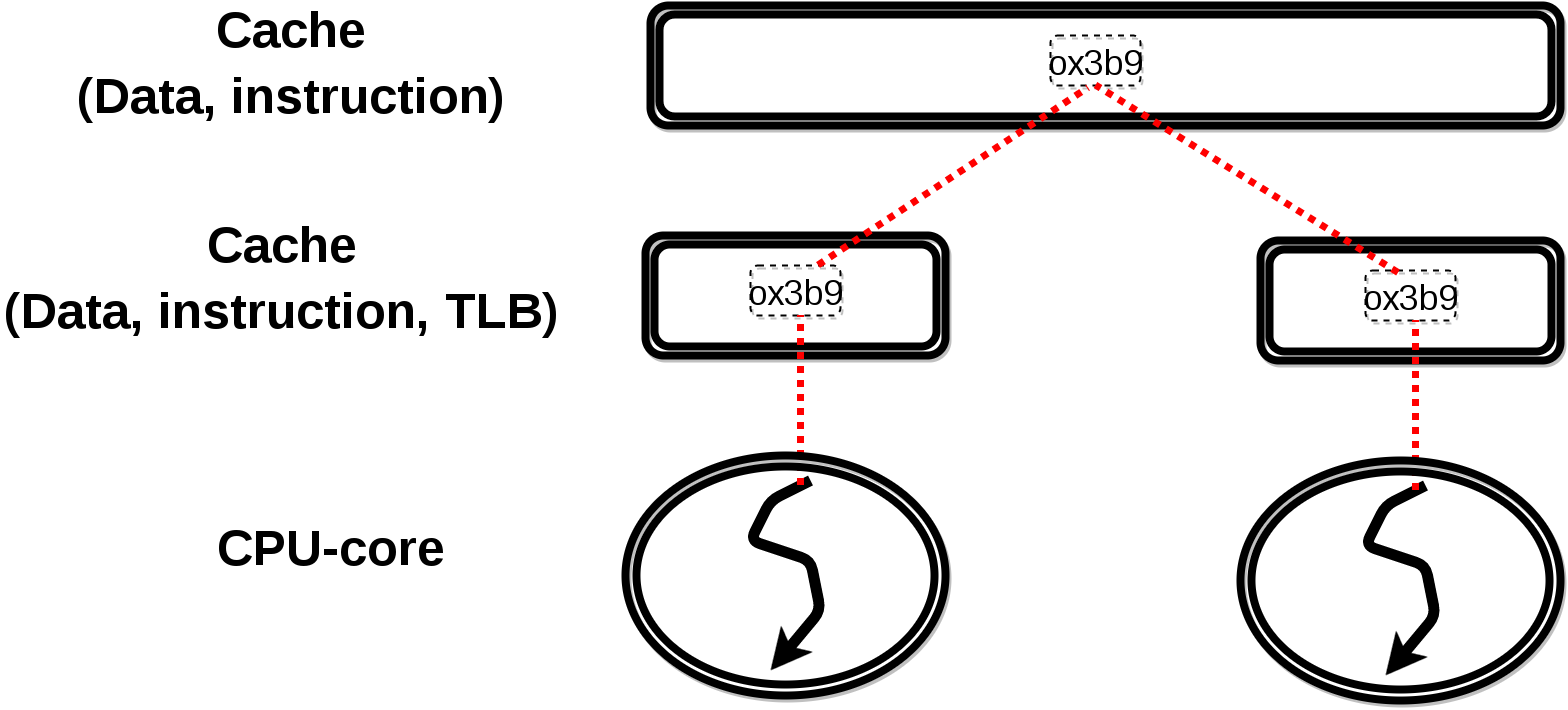
\includegraphics[width=\textwidth]{charts/internshipJulich_multicore.png}}
					\caption[]%
					{{\small Multi-core}}
				\end{subfigure}
				\caption{\emph{Intel}'s Hyper-Threading technology concept}
				\label{fig:hyperThreading}
			\end{figure*}

		It is worthwhile to mention that the thread-distribution advantage brought by the \emph{Hyper-Threading} to our overlapping solution is highly random.   Moreover, it cannot be controlled nor enforced at software (user or kernel) level.   The evaluation of such an impact on our solution is out of the scope of this study.


	\subsection{Operating-system portability} \label{subsection:osPortability}
		The main family of operating-systems (OS) targeted by our research and implementations is the \emph{UNIX}-like system\cite{wikipediaUNIX} (with a primer for \emph{Gnu-Linux} OS).   The reasons for this choice are relative to both implementation-compatibility and kernel-level requirements.\\

		%****************** Most of the HPC ecosystem is UNIX-compatible
		On one hand, our global project (\emph{Scalasca}) aims to develop an HPC utility (\toolTargetSoftware).   As a matter of fact, the HPC ecosystem is well known for its dependency on UNIX-like systems.   To the best of our knowledge, only few alternative systems\footnote{The main example is the \emph{Microsoft Windows} HPC Pack 2008.   But even this project has been dropped by \emph{Microsoft} and is no longer supported} exist for the UNIX-dominated HPC market.   No future evolutions seem likely to affect this trend.   Consequently, deploying our version of the \toolTargetSoftware\space on non \emph{UNIX}-like systems would have no real practical interest.   Such a release would target an insignificant set of potential users.\\

		%****************** Pur implementation uses UNIX-specific mechanisms
		On the other hand, the whole idea beneath our asynchronous approach is based on mechanisms that are generally specific to \emph{UNIX} architectures.   For instance, let us consider the synchronization that we have implemented between the \notationaioComputeThread\space and the \notationaioWriteThreads\space (see Section \ref{subsection:synchronization}).   Our intend was to reduce the memory footprint and ease the communication between the producer and consumers of the \notationIO\space requests.   To do so, we have made use of interprocess signals as well as condition pipes: event-driven communication.   Such a programming paradigm is intrinsically linked to the process-design of \emph{UNIX} platforms;   hence the difficulty to consider this paradigm for non-\emph{UNIX} deployment.\\
		Some state-of-the-art libraries allow to emulate \emph{UNIX}-specific mechanisms on non \emph{UNIX} platforms \cite{robison2012cilk}.   However, such solutions are not natively implemented by these systems\footnote{Unlike the signal and all event-driven mechanisms on \emph{UNIX}-compatible OS (implemented and executed at kernel level)}.   Thus, their usage may lead to a significant time and memory overhead due to extra system-calls and interprocess polling;  not to mention the obvious library- and name-space-compatibility issues.\\

		Despite this compatibility limitation, we still have considered \emph{windows}-OS portability for our implementation of the \toolTargetSoftware.\\
		% ******************Issue on windows
		The main issue when we consider deploying a multithreaded \emph{UNIX}-based application on \emph{windows} comes from the thread-synchronization:   unlike most \emph{UNIX}-based OS architectures, the \emph{windows} OS does not natively implement signals and related event-oriented mechanisms.   Thus, the whole work-flow of our multithreaded algorithm can no longer be implemented.\\
		% ******************Considered solution
		Our solution to deploy the \toolTargetSoftware\space on \emph{windows} platforms was to use the \emph{Cilk Plus}\cite{robison2012cilk} library \footnote{Library proposed by \emph{Intel} to emulate \emph{UNIX} process and relative thread-synchronization mechanisms on \emph{windows} platforms at user level (user mode)}.   Then, through a custom wrapper of this library, we have been able to fit all the kernel-level requirements of our algorithms and benchmarks.   Using this wrapper, we have also limited the engineering effort by adapting this interface to the standards followed by the \toolTargetSoftware\space (name spaces, function names and parameters).\\
		% ******************Potential limitation of the solution
		This kind of user-level emulation of a kernel process is well known for its potential performance downgrade\cite{tousimojarad2014comparison}.   Indeed, the \emph{Cilk Plus} library manages the process address-space (and principally the heap's dynamic memory) through costly system calls to the host kernel (instead of being natively executed by the kernel).   Likewise, the implementation of these signals and these synchronizations is based on \emph{active-waiting} and \emph{polling}.\\
		The assessment of such an overhead on our asynchronous approach (deployed on \emph{windows} OS) is beyond the scope of this work.\\

		For simplicity and clearness, all the considered implementations in the rest of this work will be implicitly developed, implemented and assessed on UNIX platforms.


	\subsection{Experimental setup}\label{section:experimentalSetup}
		% ****************** Hardware platform: HPC (Processor + disk)
		The experimental evaluations that will be presented in the next chapter have been obtained on two x86 machines.\\
		The first one is a \emph{JURECA T-Platforms V-Class} (HPC) consisting of two 24-core (\targetPlatformHpcProcessor\space (\targetPlatformHpcFrequency) \emph{Haswell}) chips.   Each core has a double physical thread support (\emph{Hyper-Threading}).   The machine accesses its \notationIO\space resource using \emph{JUST}\cite{just}: a \emph{General-Parallel-File-System} storage cluster.   Thanks to the hardware distribution of its underlying disks, this file system may perform (\emph{physically}) several simultaneous accesses to the \notationIO\space resource.   The access to this file system is performed through a $100$ GiB/s connection.   Finally, on this machine, a \emph{Gnu-Linux} (3.10.0-514.26.2.el7) operating system has been used based on the \emph{CentOS} kernel (7.3.1611).   The default kernel dynamic memory allocation policy (\emph{first touch}) has been set.\\
		For all the presented experimentations on the \emph{JURECA HPC} nor intermediate virtualization, or job-encapsulation\footnote{Using jobs (through a batch scheduler) is a standard way to access an HPC or a cluster platform} has been used.\\

		% ****************** Hardware platform: workstation (Processor + disk)
		The second considered machine is an \emph{ASUS M32CD-US014T} consisting of four 2-core (\targetPlatformLaptop\space (\targetPlatformLaptopFrequency)) chips.   Each core has a double physical thread-support (\emph{Hyper-Threading}).   All the \notationIO\space accesses on this machine have been performed on a single disk (\emph{Samsung SSD 850-EVO, 2.5" ATA}) of $256$ GiB.   To the best of our knowledge, no specific hardware or software optimization has been used regarding this disk.   Finally, on this machine, a \emph{Gnu-Linux} (4.4.74-18.20) operating system has been used based on the \emph{openSUSE} kernel (\emph{Leap} 42.2).   The default kernel dynamic memory allocation policy (first touch) has been set.\\

		% ****************** g++ and score-p
		All the programs that implement our algorithms of the \toolTargetSoftware\space and the \toolSimulationSoftware\space have been implemented in C++ language (using the ISO C++11 standard).   They have been compiled using \textit{g++} (\emph{GCC} 5.4.0).  The option -O3 (maximum optimization level) has been used for all the compilation processes.   Additionally, the compiler has been coupled with the \toolProfiling\space (4.0-orphaned-pthreads) to inject the performance-profiling routines to the assessed applications (see Section \ref{section:executionProfiling}).   A custom patch of \toolProfiling\space has been implemented in order to profile asynchronous signal-handler.\\

		% ****************** Cube, the existing Cube-remapper and our custom code
		Finally, the software we are trying to outperform is the \toolTargetSoftware\space (part of the \toolTraceAnalyzed\space (4.4)).   This version of the \toolTargetSoftware\space has been used as a performance-benchmark to test our custom implementations.   It has also been used as a basis to our custom implementation of the \toolTargetSoftware.\\

		% ****************** Why using 2 hardware platform (confirm results are not just due to HPC performance)
		Although the \emph{JURECA HPC} has been used to evaluate our approach, we have still confirmed our observations on a regular workstation (\emph{ASUS} \targetPlatformLaptop).   We have dedicated our effort to separate as much as possible the performance gain brought by our design from the hardware performance of this HPC.   Consequently, the observed experimental gain, which will be highlighted in the next chapter, is not simply due to the performance of the storage cluster on the considered HPC.




%This chapter present and discuss the research results, respectively.
%They are often usefully combined into one section, however, because readers can seldom make sense of results alone without accompanying interpretation.
%They need to be told what the results mean.



\chapter{Results and Discussion}\label{chapter:results}
	In this chapter, we use our custom simulation test-bed to assess the models we presented in both synchronous and asynchronous cases.   In Section \ref{section:asynchronousModel}, we evaluate the accuracy of these models.   We also give an experimental evaluation of the gain brought by our solutions on the considered pattern.\\
	In Section \ref{section:experimentalCase}, we compare the performances of our \notationaio\space solution using both our \toolSimulationSoftware\space and our custom implementation of the \toolTargetSoftware.   We show how our solution might interfere with a real-life application (namely: the \toolTargetSoftware software).   We show how we identified the causes of these different perturbations.   We also evaluate the sequence of custom solutions that lighten such perturbations.\\


%--------------------------------------------
\section{Asynchronous model and improvements} \label{section:asynchronousModel}
	\subsection{First model assessment (single \notationIO\space device)}\label{subsection:AIO_firstApproachAssessment}
		In order to assess the first theoretical model (see Section \ref{subsection:firstModel}), one should first be able to assess the \emph{write} time $W$ of each buffer.   According to the model hypotheses, this \emph{write} time is considered as constant (for a fixed data size and a given hardware platform).   Figure \ref{fig:writeTimeExample} shows the experimental evaluation that we have obtained on the two considered platforms.\\

			\begin{figure*}[!h]
				\centering
				\begin{subfigure}[b]{0.475\textwidth}
					\centering
					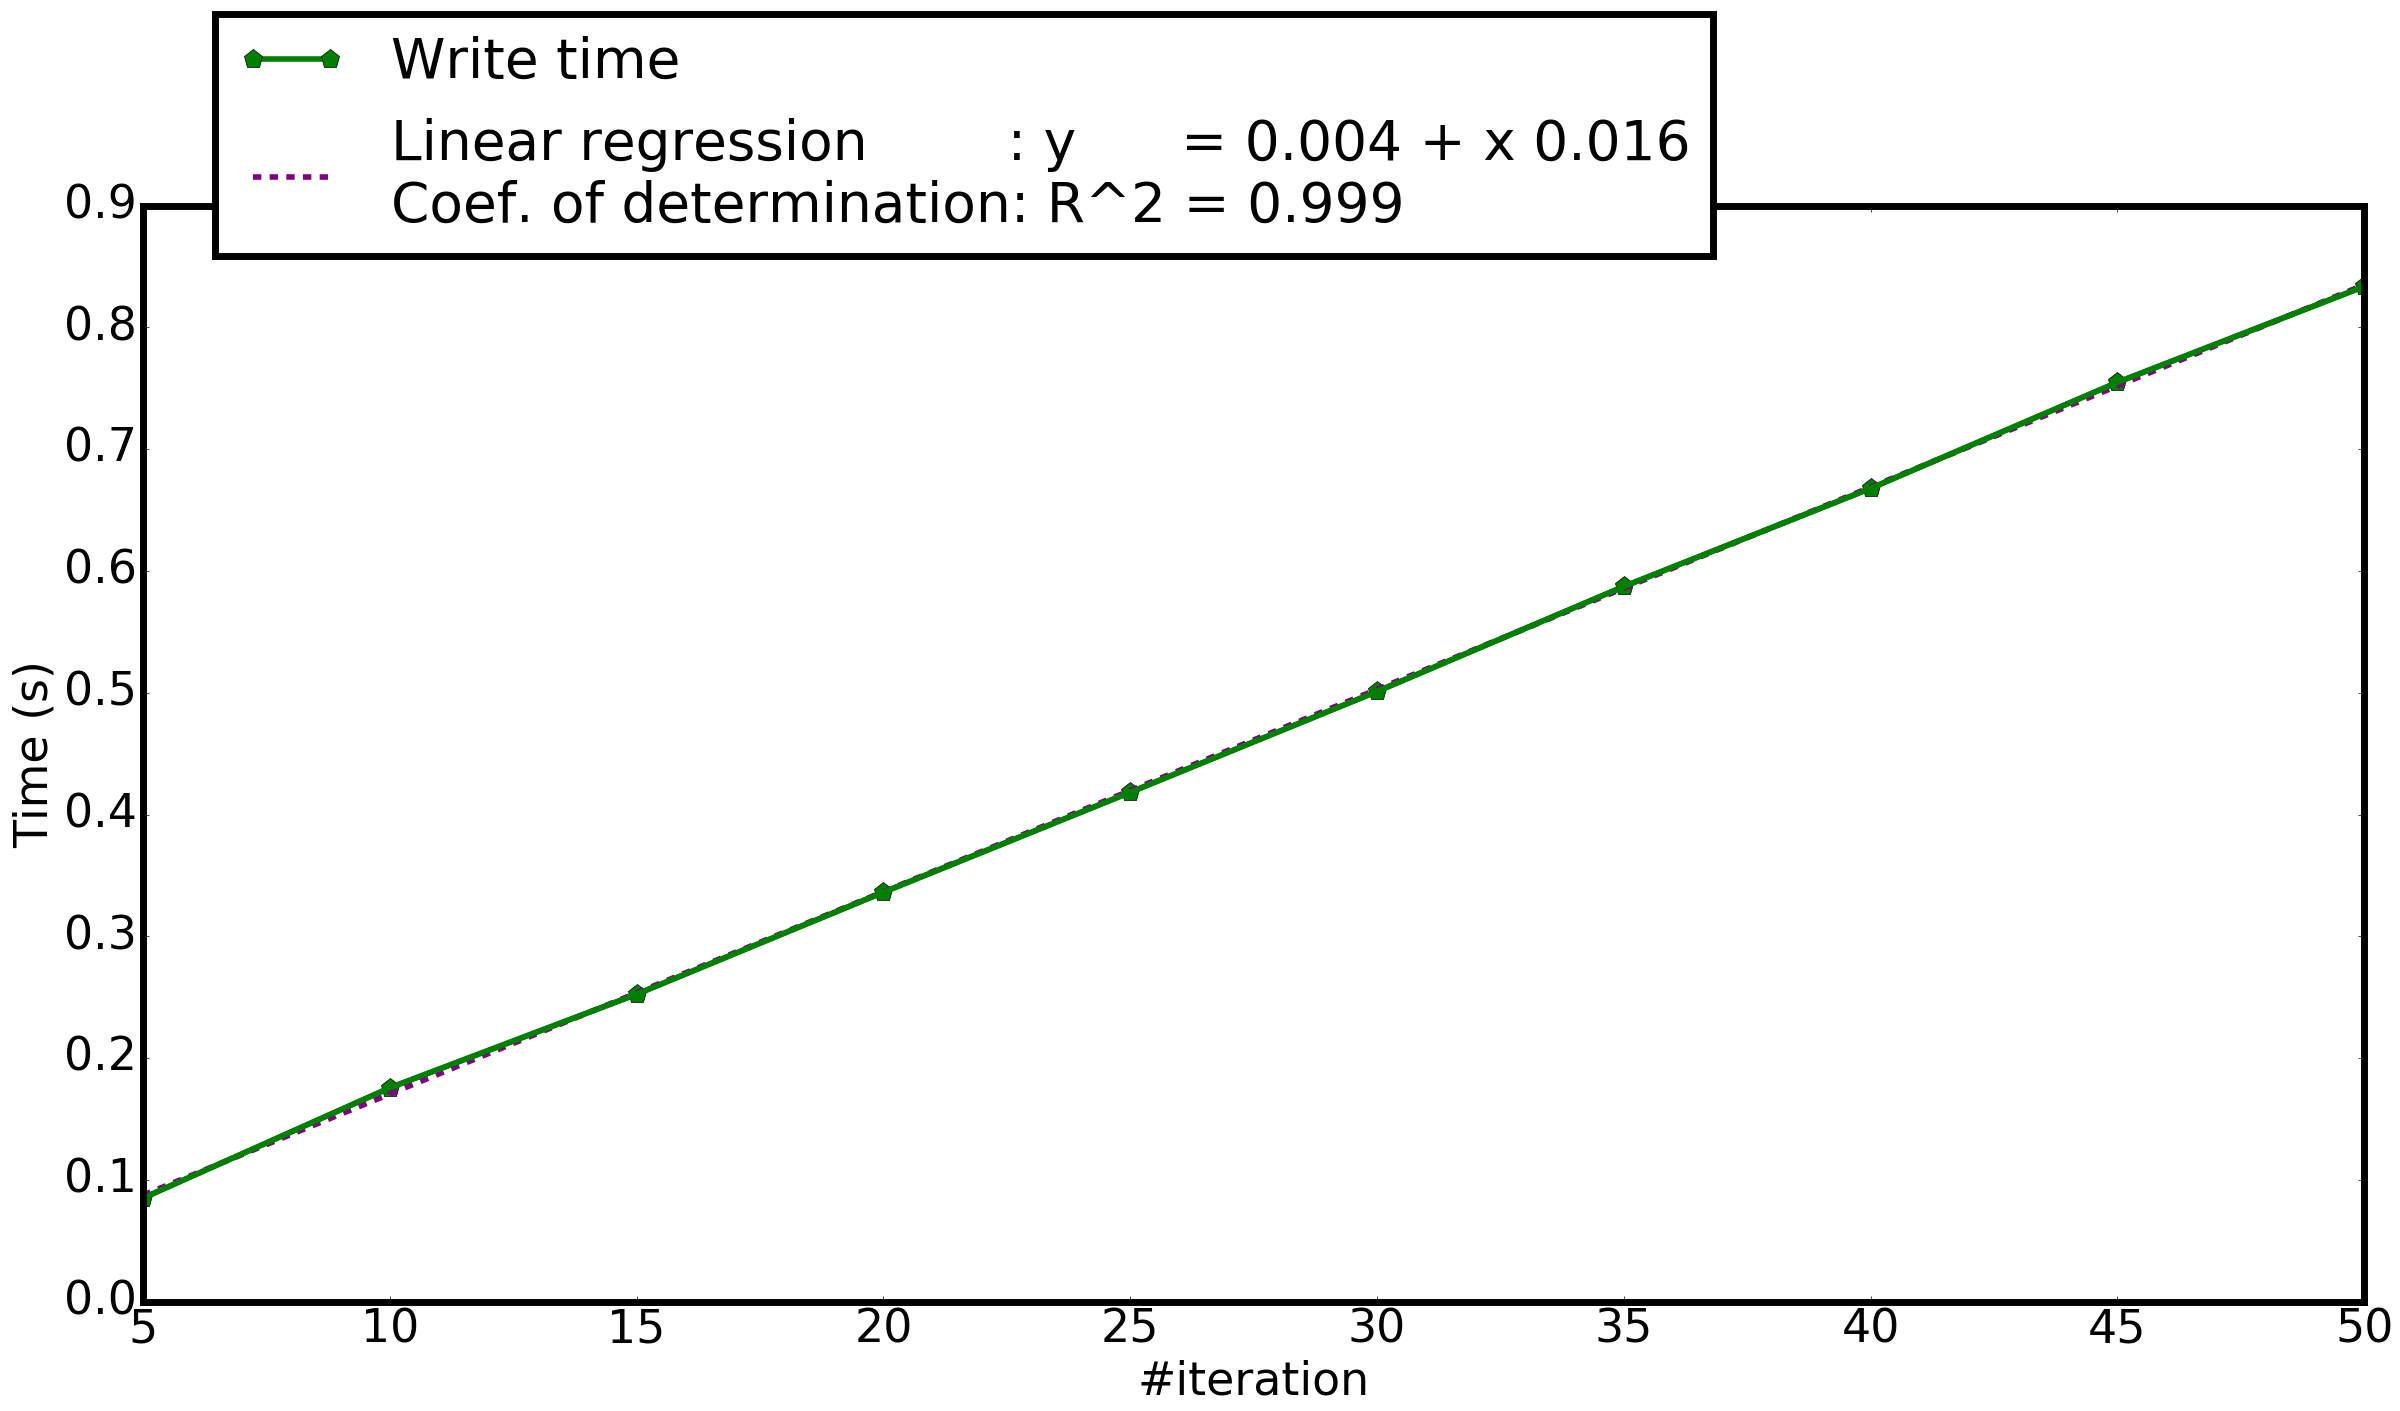
\includegraphics[width=\textwidth]{charts/writeTimeExample_workstation_8core.png}
					\caption[\targetPlatformLaptop \space @ \targetPlatformLaptopFrequency]
					{{\small \targetPlatformLaptop \space @ \targetPlatformLaptopFrequency}}
					\label{fig:writeTimeExample_workstation}
				\end{subfigure}
				\hfill
				\begin{subfigure}[b]{0.475\textwidth}  
					\centering 
					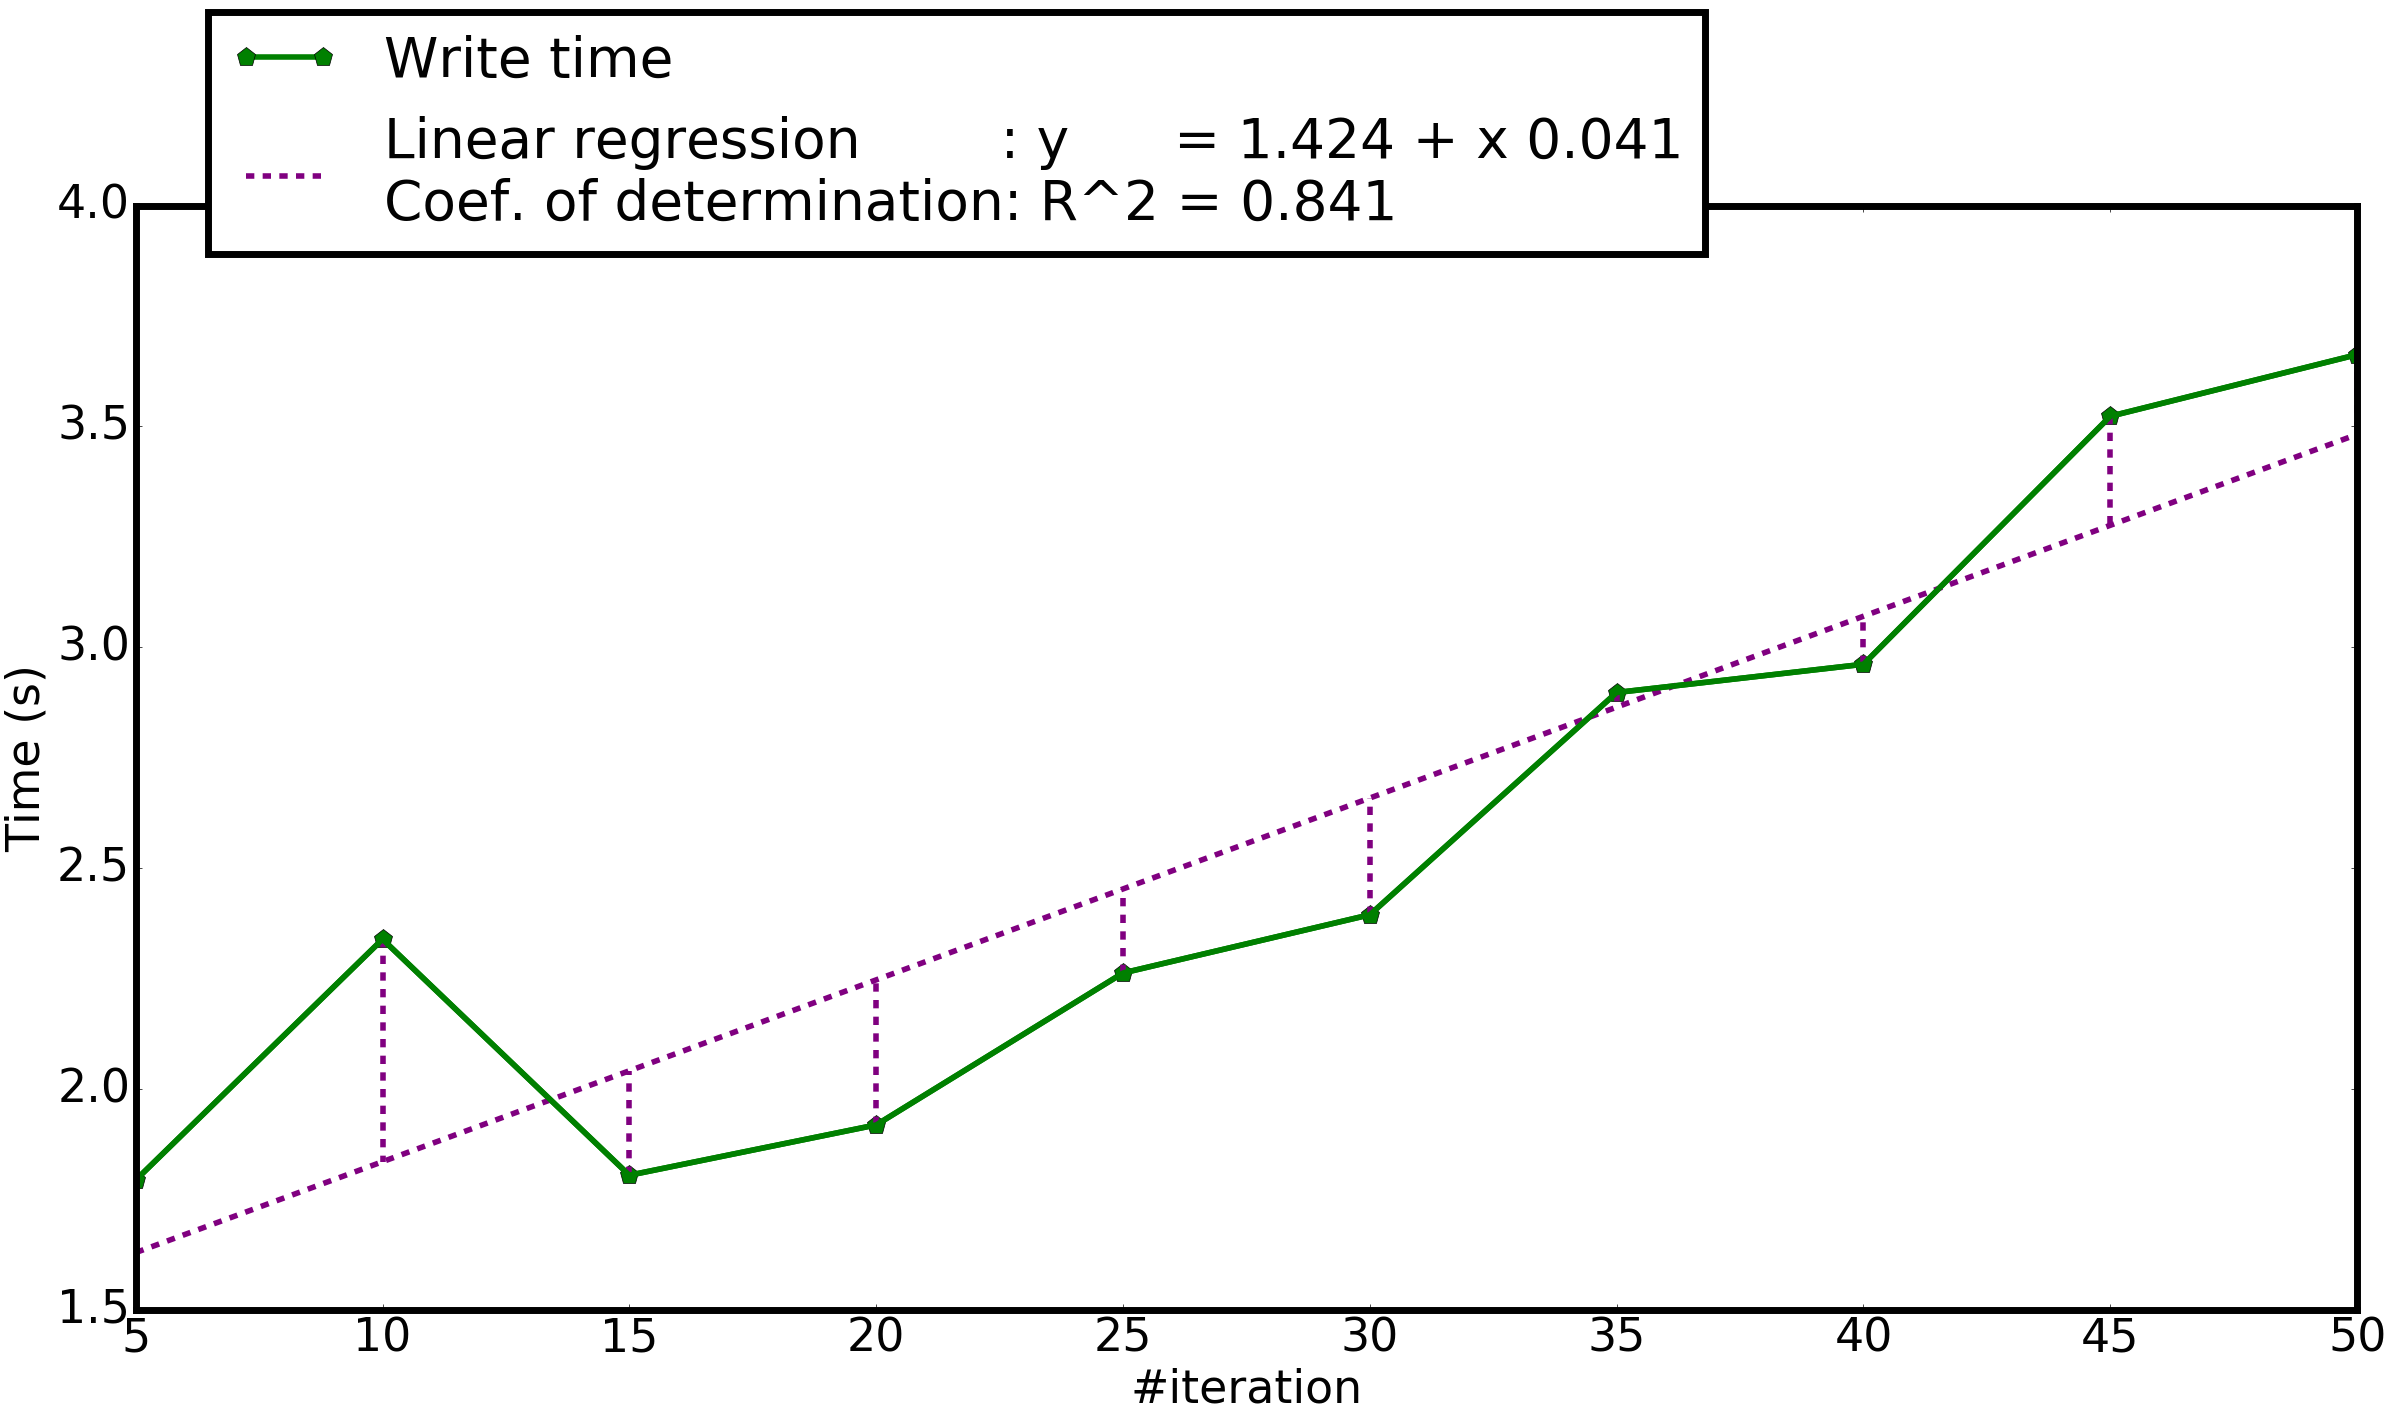
\includegraphics[width=\textwidth]{charts/writeTimeExample_HPC_jureca.png}
					\caption[]%
					{{\small \targetPlatformHpc \space @ \targetPlatformHpcFrequency}}    
					\label{fig:writeTimeExample_hpc}
				\end{subfigure}
				\caption{Experimental assessment of the time for writing 50,000,000 bytes}
				\label{fig:writeTimeExample}
			\end{figure*}

		One could notice on these experimental results that the assessed \emph{write} time is roughly constant through different assessments (excluding the outliers which are regularly observed at the beginning of each experimentation on the HPC platform\footnote{This outlier corresponds probably to a warm-up phase before the pre-loader of the \notationIO\space device becomes fully efficient (for the currently accessed \notationIO\space pattern)}).   Indeed, the value of the \emph{write} time $W$ fluctuates within a range of $10 ^{-2}$ seconds (for both considered hardware platforms).   As the measured computation times ($C$) fluctuates within a higher range of $10^{-1}$ seconds (see Section \ref{section:experimentalCase}), then the variation of $W$ could be considered as comparatively negligible.   The retained \emph{write} time approximation is the slope of the linear regression on Figure \ref{fig:writeTimeExample}.   This value (for writing $50,000,000$ bytes) is $W=0.016$ seconds for the \targetPlatformLaptop\space (Figure \ref{fig:writeTimeExample_workstation}) and $W=0.041$ seconds for the \targetPlatformHpc\space (Figure \ref{fig:writeTimeExample_hpc}).\\

		Using the simulation test-bed described in Section \ref{subsection:simulationTestbed}, we compared the asynchronous implementation with the synchronous one and the theoretical model (see Figure \ref{fig:model0_assessment}).\\
			\begin{figure*}[!h]
				\centering
				\begin{subfigure}[b]{0.475\textwidth}
					\centering
					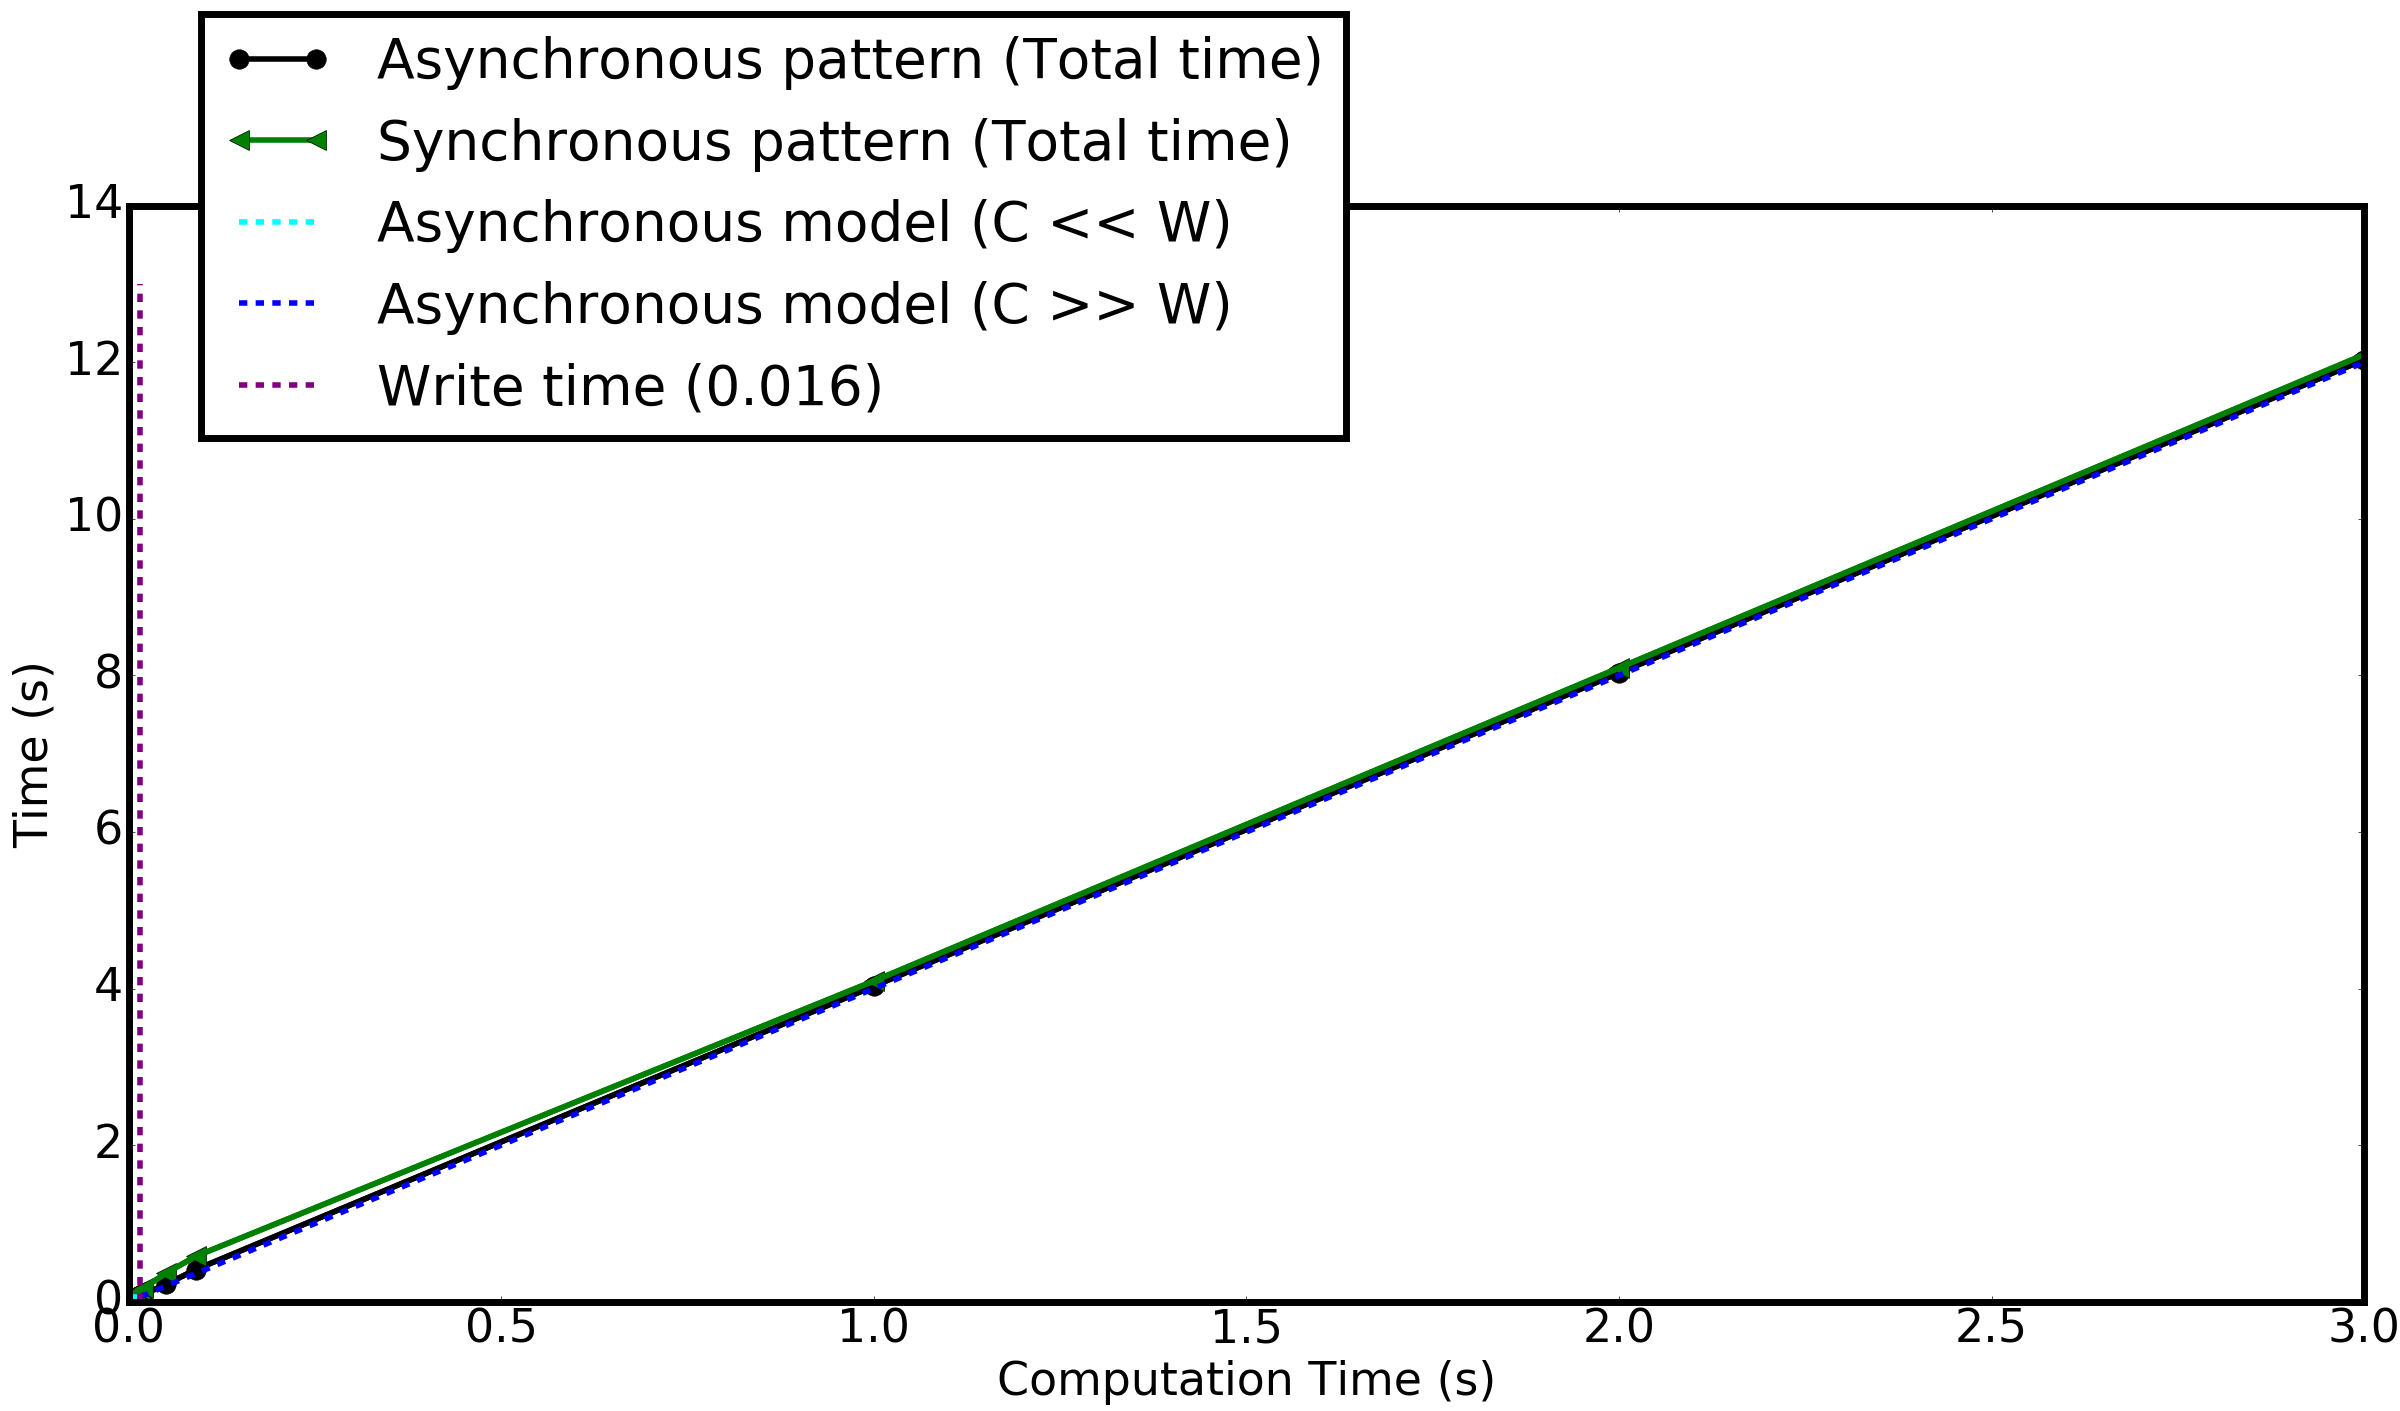
\includegraphics[width=\textwidth]{charts/model0_workstation_8core.png}
					\caption[\targetPlatformLaptop \space @ \targetPlatformLaptopFrequency\space (Linear scale)]%
					{{\small \targetPlatformLaptop \space @ \targetPlatformLaptopFrequency\space (Linear scale)}}
					\label{fig:model0_assessment_laptop}
				\end{subfigure}
				\hfill
				\begin{subfigure}[b]{0.475\textwidth}
					\centering
					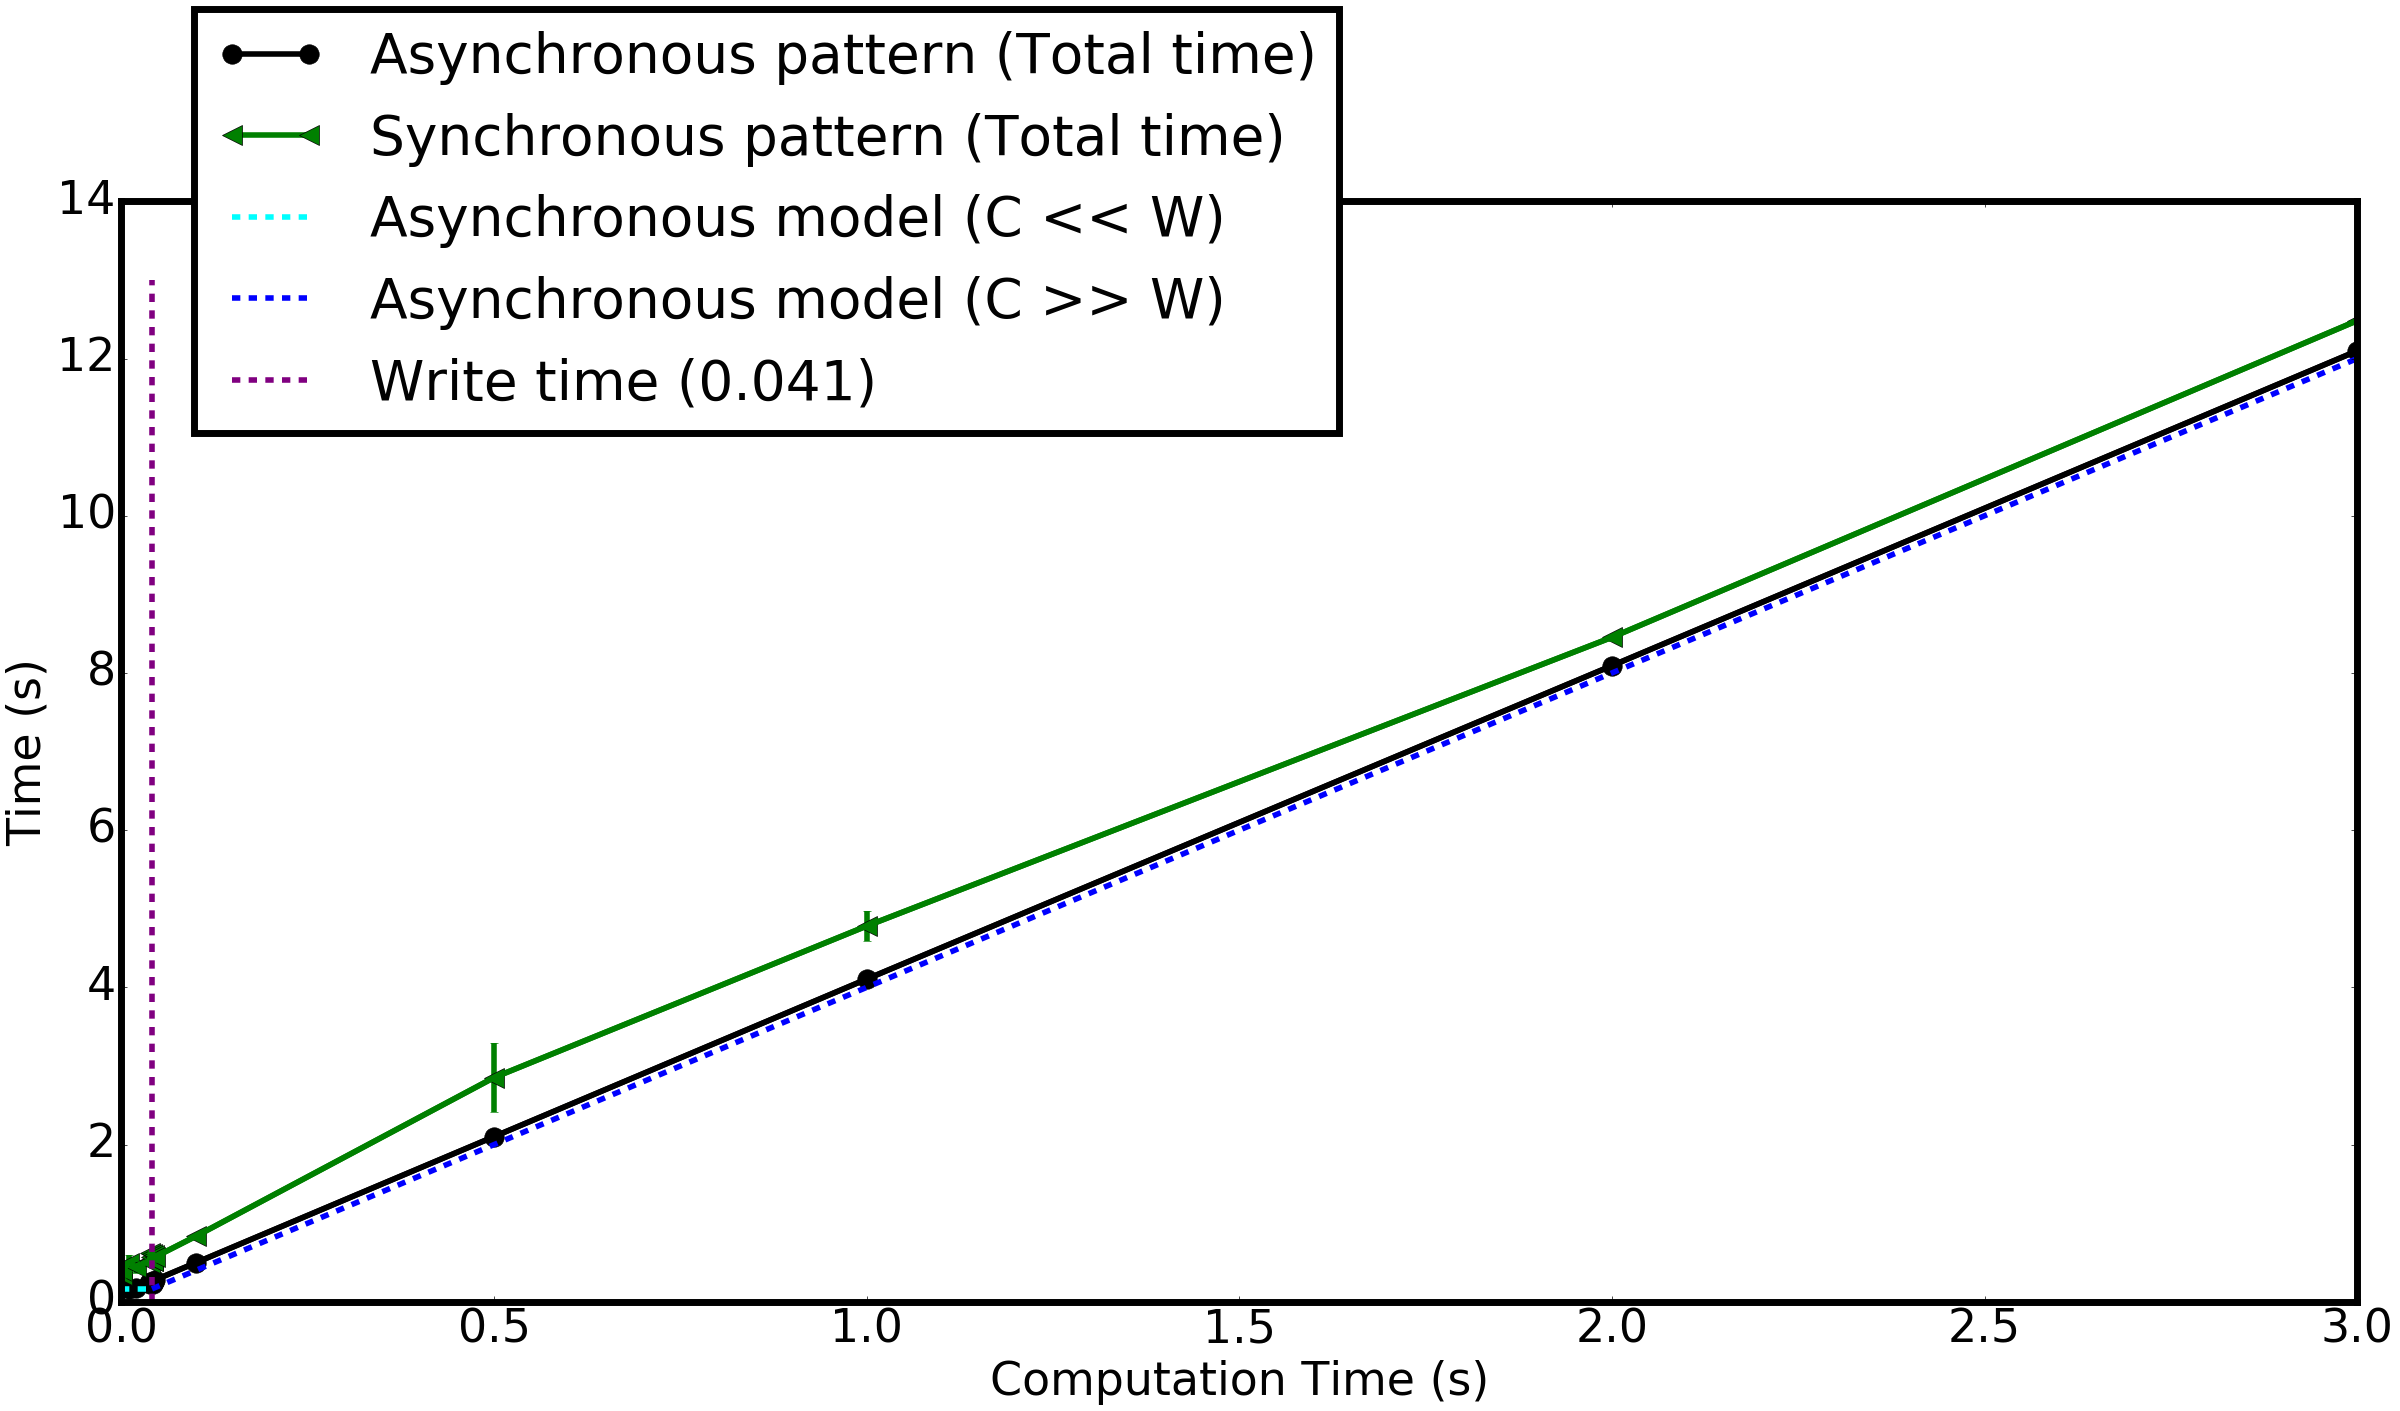
\includegraphics[width=\textwidth]{charts/model0_hpc_2Proc_1IoDevice.png}
					\caption[]%
					{{\small \targetPlatformHpc \space @ \targetPlatformHpcFrequency\space (Linear scale)}}
					\label{fig:model0_assessment_hpc}
				\end{subfigure}
				\vskip\baselineskip
				\begin{subfigure}[b]{0.475\textwidth}  
					\centering 
					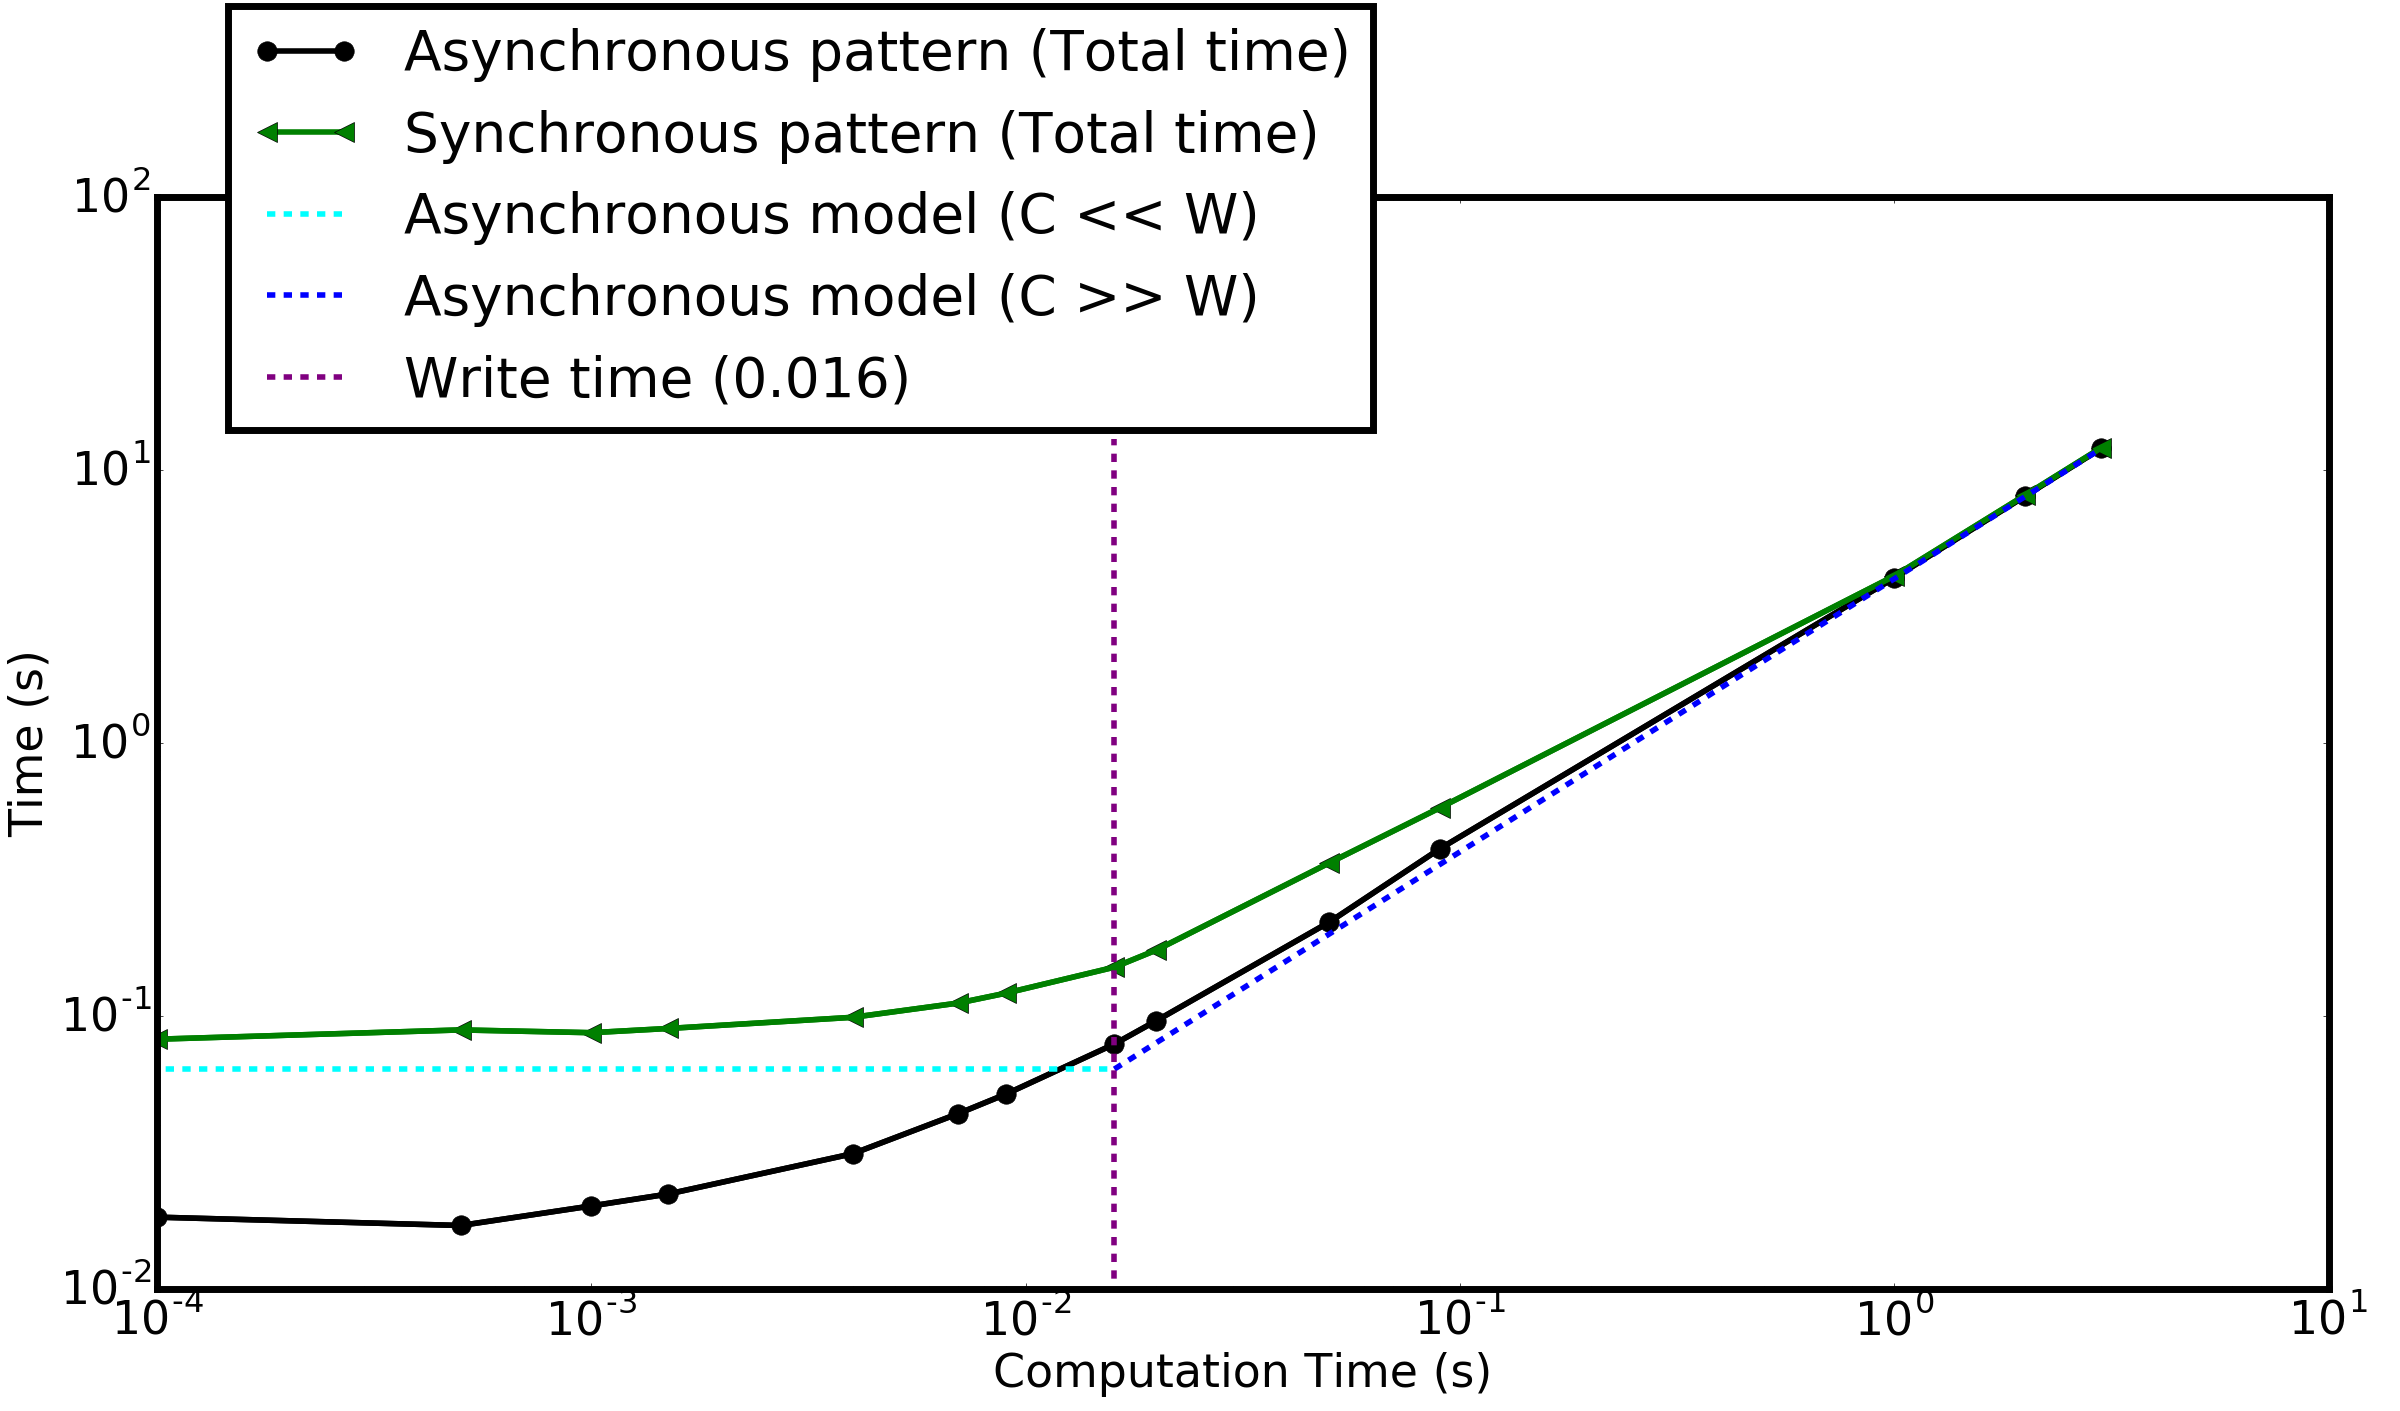
\includegraphics[width=\textwidth]{charts/model0_workstation_8core_logScale.png}
					\caption[]%
					{{\small \targetPlatformLaptop \space @ \targetPlatformLaptopFrequency\space (Log-Log scale)}}
					\label{fig:model0_assessment_laptop_log}
				\end{subfigure}
				\hfill
				\begin{subfigure}[b]{0.475\textwidth}  
					\centering 
					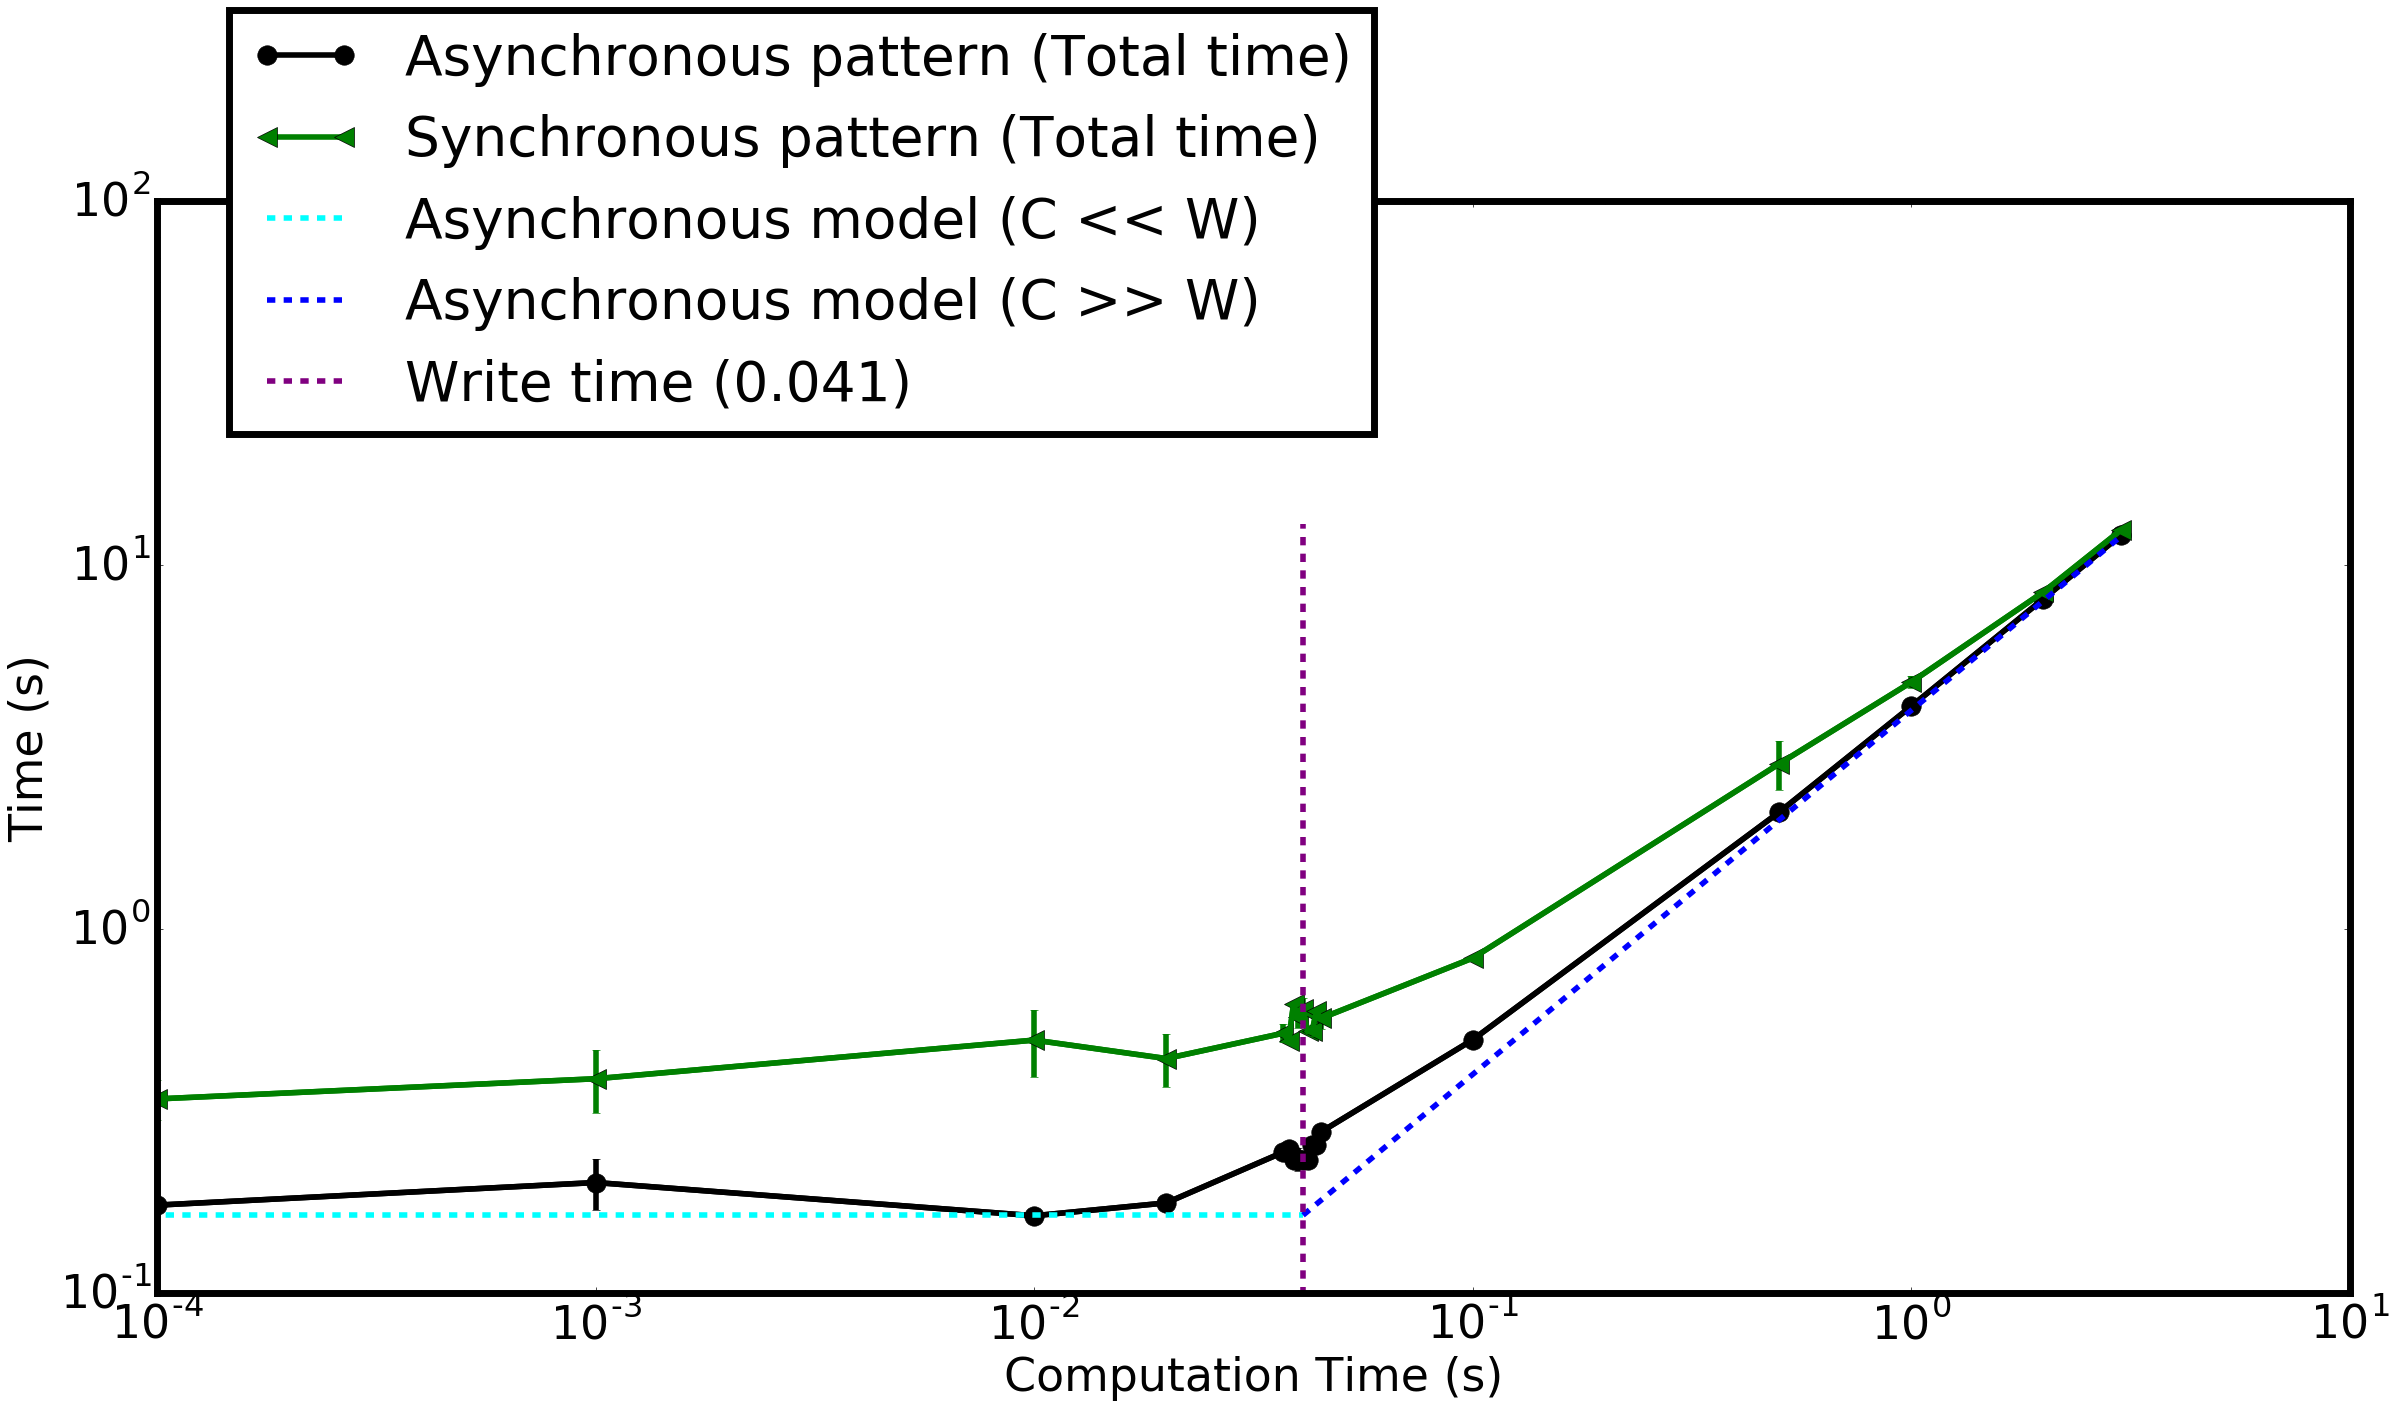
\includegraphics[width=\textwidth]{charts/model0_hpc_2Proc_1IoDevice_logScale.png}
					\caption[]%
					{{\small \targetPlatformHpc \space @ \targetPlatformHpcFrequency\space (Log-Log scale)}}
					\label{fig:model0_assessment_hpc_log}
				\end{subfigure}
				\caption{Experimental comparison of the asynchronous solution with its theoretical model and the synchronous one (50,000,000 bytes per write, 4 iterations)}
				\label{fig:model0_assessment}
			\end{figure*}

		First of all, it is clear on Figure \ref{fig:model0_assessment} that, on both targeted platforms, our custom \notationaio\space \emph{write} approach might bring a significant improvement compared to the original synchronous one.   When the computation time is in the neighbourhood of the \emph{write} time, an improvement up to $45\%$ is observed on the \targetPlatformLaptop\space and $38\%$ on the \targetPlatformHpc).   Hence, our global approach to optimize the \toolTargetSoftware\space seems comforted at this stage.\\
		Second, the trends modelled by Equations (\ref{equation:synchronousModel}) and (\ref{equation:model0}) are clearly highlighted and matched by the experimental response times of the considered pattern on Figure \ref{fig:model0_assessment}.   We can notice the accuracy in the position of the inflection point on both targeted platforms.\\

		Finally, Figure \ref{fig:model0_assessment} allows to identify the region\footnote{Set of computation times} where the improvement brought by our \notationaio\space \emph{write} algorithm is the most significant.   Indeed, we can notice on both platforms that this gain is maximal when the \emph{compute} time is in the neighbourhood of the \emph{write} time.\\

		Such a property of our \notationaio\space approach is complicated to use in a real-life software (such as the \toolTargetSoftware).   As a matter of fact, it is not easy to adapt the \emph{compute} function and make its execution time match a given value.   Furthermore, this targeted value of the \emph{compute} time is totally dependent on the host hardware platform.\\
		However, this property might be used to analyse the performance of the considered software (once shipped with our solution).   A \emph{compute} time that is too far from the \emph{write} time could lead to a poor performance-gain of our solution.


	\subsection{Second model assessment (single \notationIO\space device)} 
		We notice on Figure \ref{fig:model0_assessment} that, in one case (\targetPlatformLaptop), the predictions of our first asynchronous model (Equation (\ref{equation:model0})) are well-confirmed by the experimental results (Figures \ref{fig:model0_assessment_hpc} and \ref{fig:model0_assessment_hpc_log}).   This is however not always the case as Figures \ref{fig:model0_assessment_laptop} and \ref{fig:model0_assessment_laptop_log} exhibit a significant gap between the theoretical model and the experiment for the \targetPlatformLaptop\space hardware.\\
		One could notice that this deviation seems roughly constant\footnote{Does not depend on the computation time} (for $C<<W$ and $C>>W$).   Therefore, the enhanced second model proposed by Equation (\ref{equation:model1}) maybe more accurate.   In this section, we experimentally test this second model by assessing its two founding parameters: the \emph{write} time ($W_{perturbation}$) and the \notationaio\space \emph{request} time ($req$).


		\subsubsection{Modelling the \emph{write} time ($W_{perturbation}$)}
			The experimental approximation of the \emph{write} time previously presented (Section \ref{subsection:AIO_firstApproachAssessment}) has a relatively low fitting-coefficient\footnote{\emph{Regression coefficient of determination $R^{2}$ of the linear model}} equal to $0.84$ on the \targetPlatformHpc\space platform (see Figure \ref{fig:writeTimeExample_hpc}).   Consequently, we have considered using the \emph{saturation method} (see Section \ref{subsubsection:modelRequestTime}) in order to attempt to model the \emph{write} time more realistically.\\

			\begin{figure*}[!h]
				\centering
				\begin{subfigure}[b]{0.475\textwidth}
					\centering
					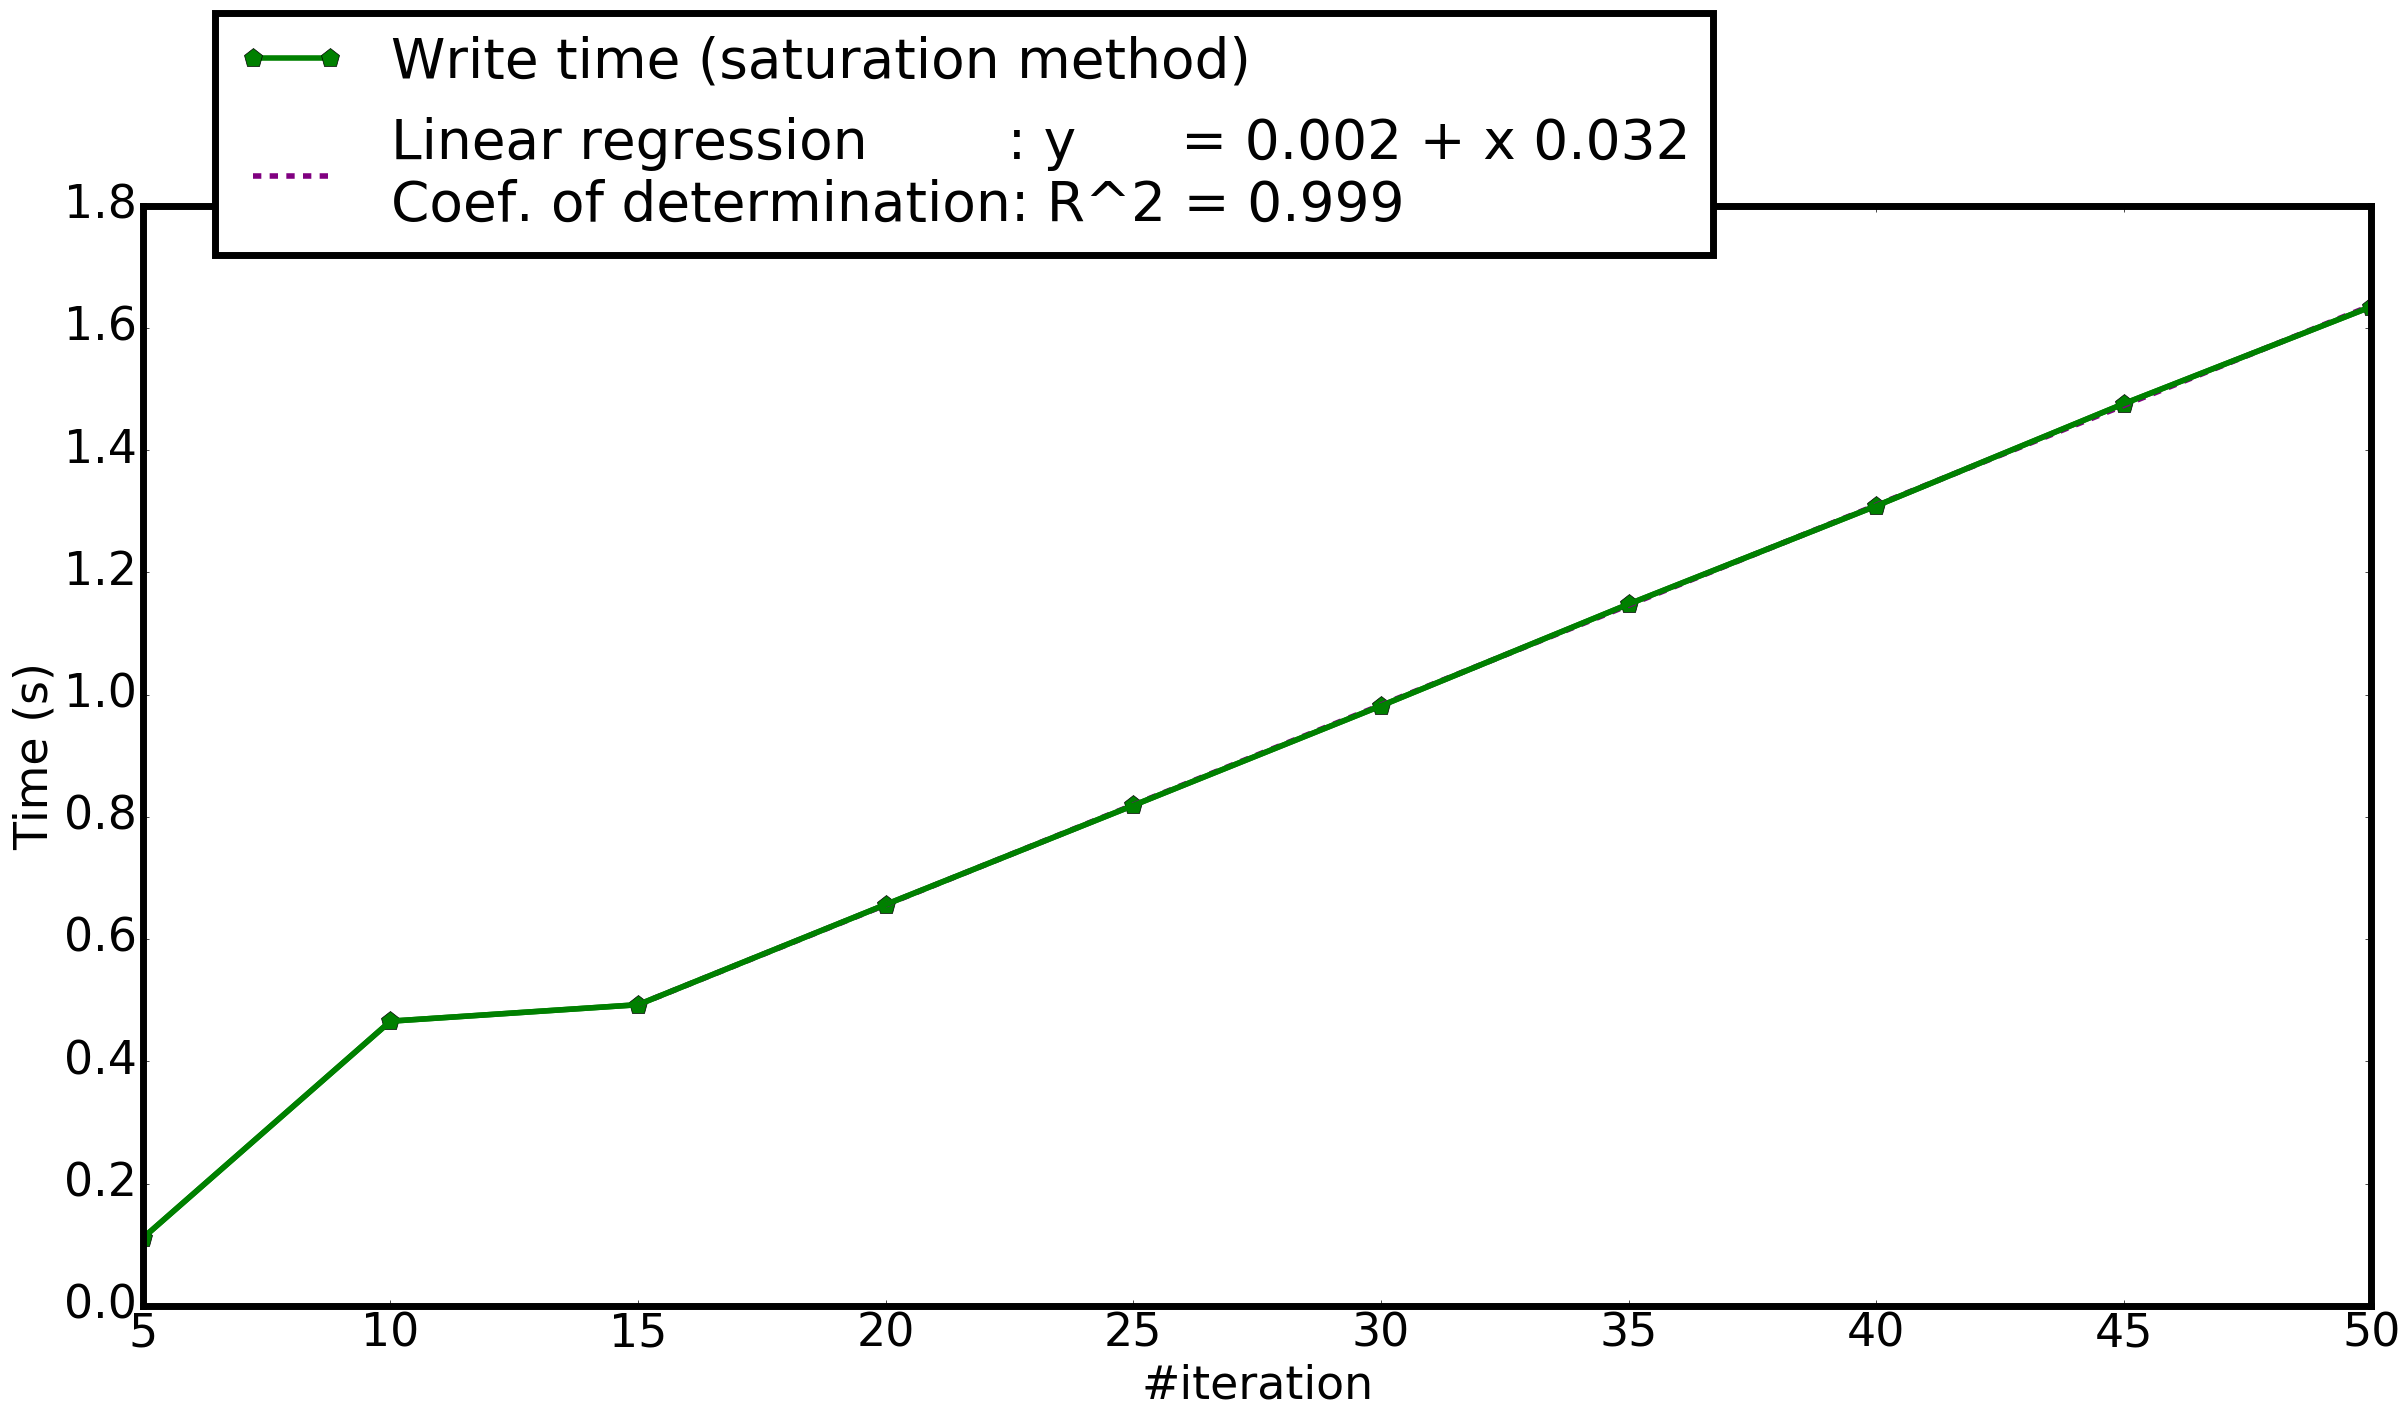
\includegraphics[width=\textwidth]{charts/writeTimeExample_saturationMethod_workstation_8core.png}
					\caption[\targetPlatformLaptop\space @ \targetPlatformLaptopFrequency]
					{{\small \targetPlatformLaptop\space @ \targetPlatformLaptopFrequency}}
				\end{subfigure}
				\hfill
				\begin{subfigure}[b]{0.475\textwidth}  
					\centering 
					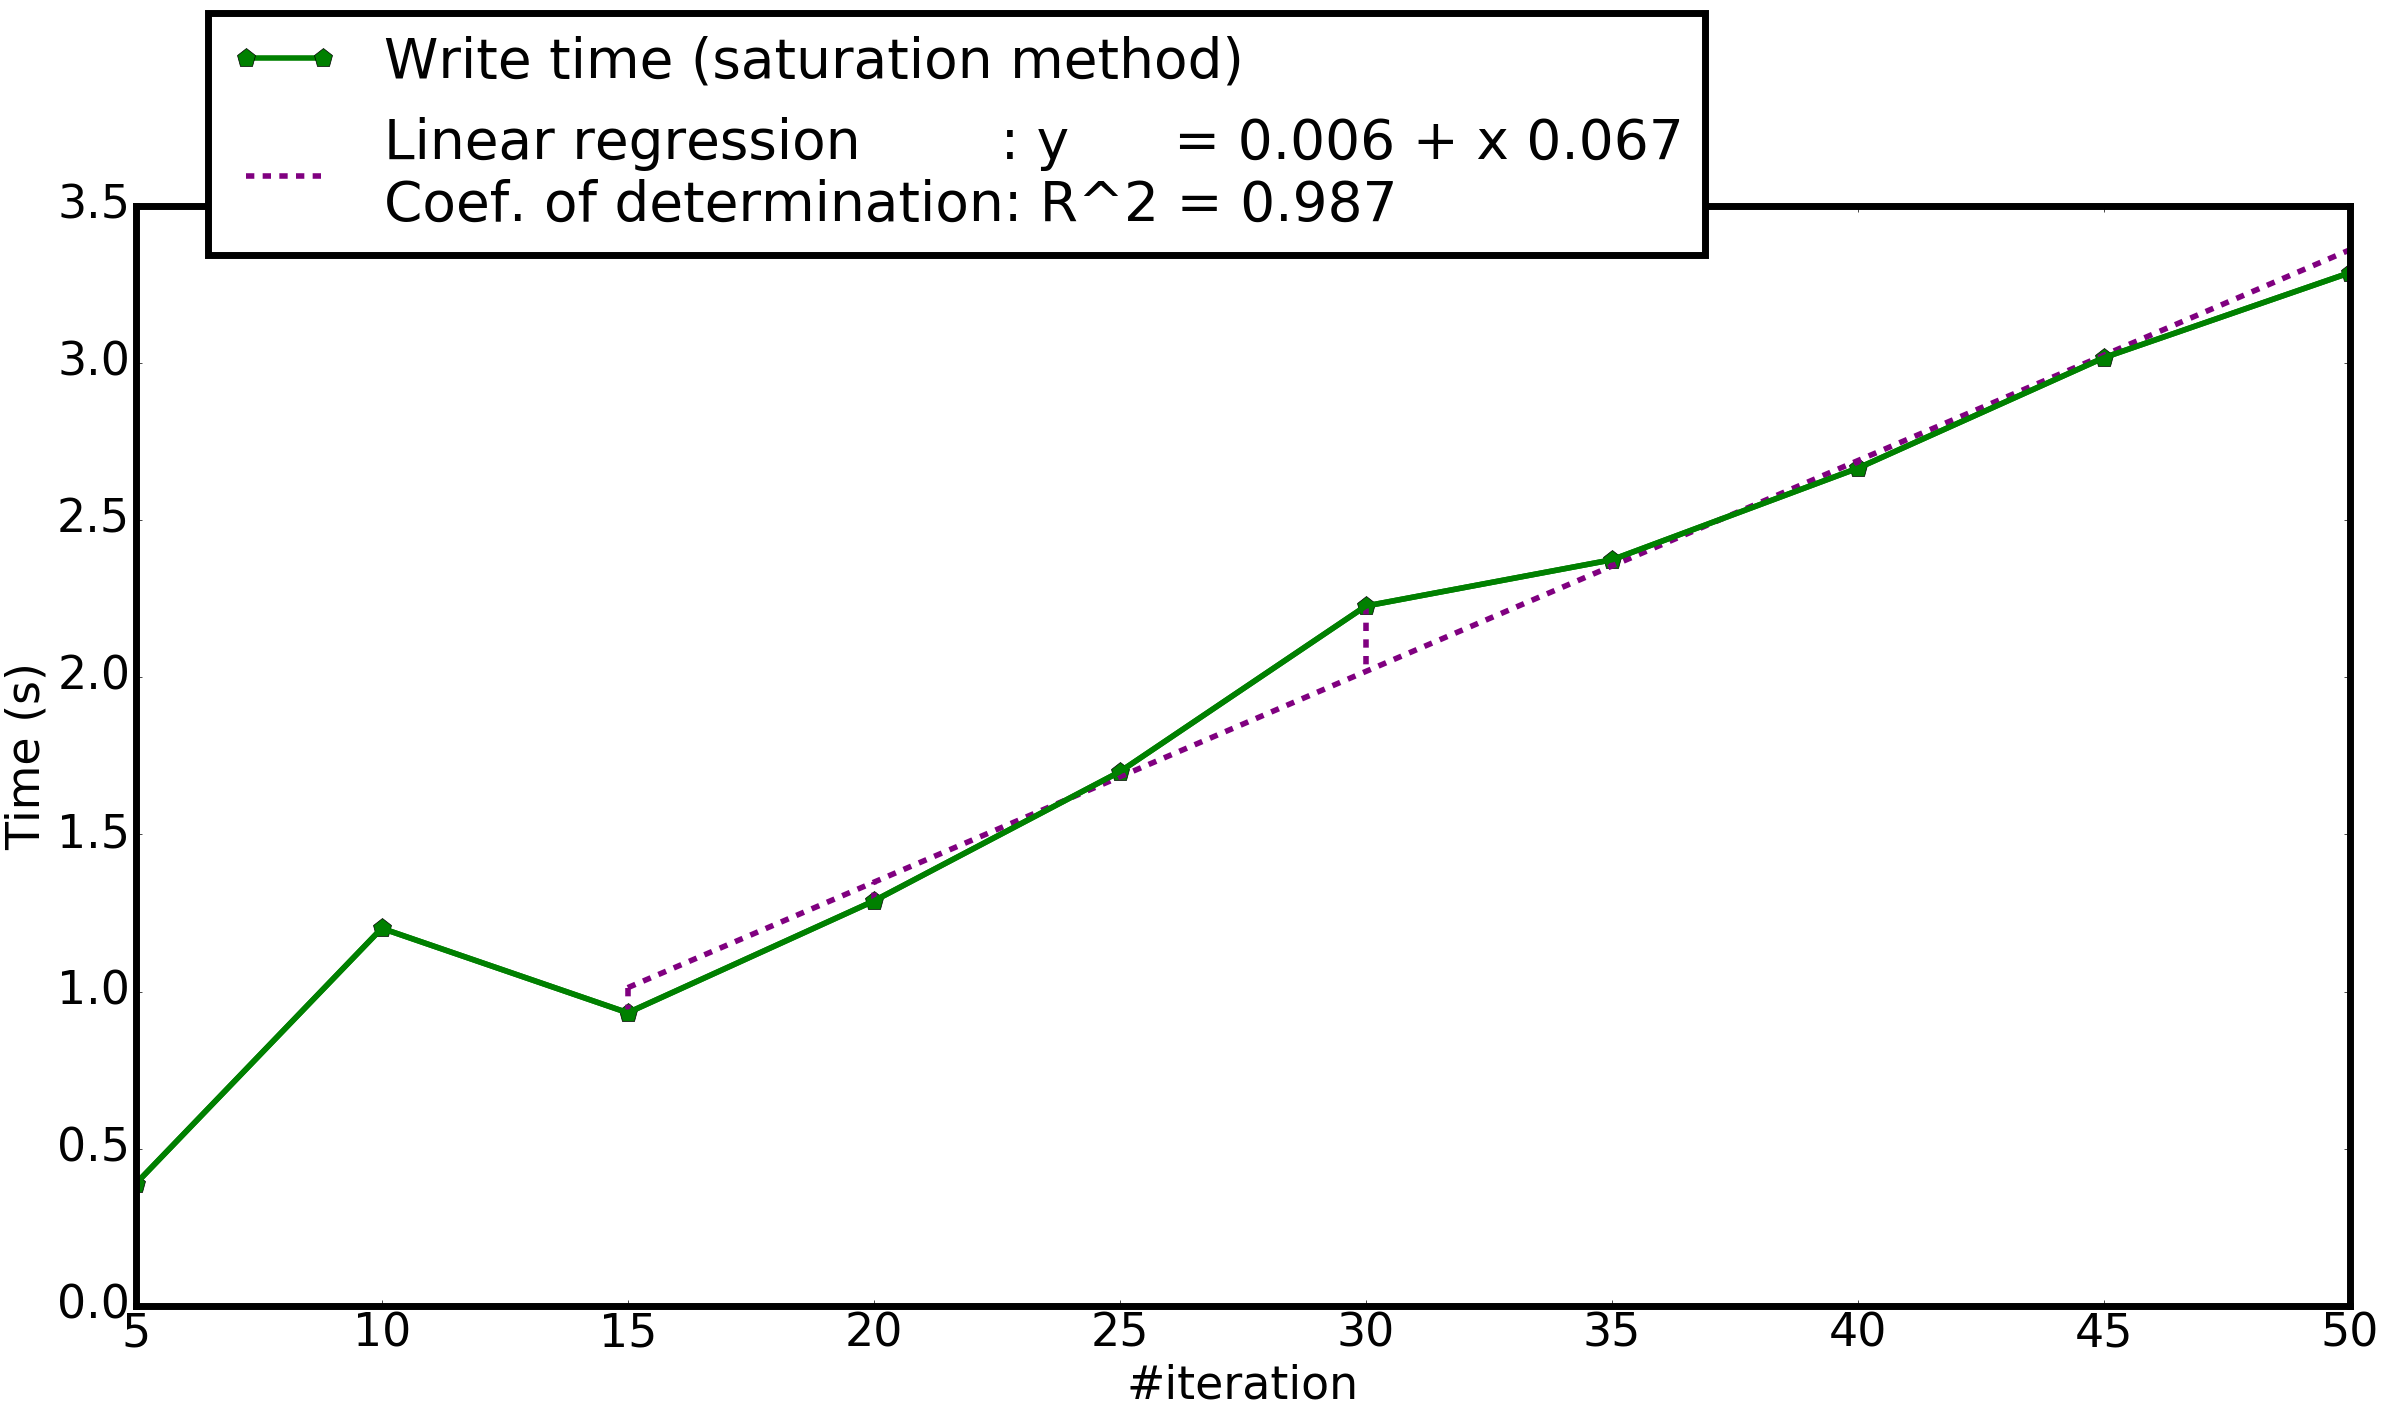
\includegraphics[width=\textwidth]{charts/writeTimeExample_saturationMethod_HPC_jureca.png}
					\caption[]%
					{{\small \targetPlatformHpc\space @ \targetPlatformHpcFrequency}}    
					\label{fig:writeTimeExample_saturation_hpc}
				\end{subfigure}
				\caption{Experimental assessment of the time for writing 50,000,000 bytes using the \emph{I/O saturation method}}
				\label{fig:writeTimeExample_saturation}
			\end{figure*}
			In Figure \ref{fig:writeTimeExample_saturation}, we have represented our measurement of the \emph{write} time ($50,000,000$ bytes) using the \emph{saturation method}.   One can notice that, after a warm-up phase\footnote{Corresponding to the time to flood the file system with \notationIO\space requests}, the \emph{write} time reaches a given threshold.   Then, its fluctuations almost vanish.\\

			Thanks to the \emph{saturation method}, the fitting-coefficient of the \emph{write} time estimation has been improved to $0.987$ (see Figure \ref{fig:writeTimeExample_saturation_hpc}) on the \targetPlatformHpc\space platform.   Furthermore, the constant term in the linear approximation of the \emph{write} time is now closer to zero ($0.006$ seconds) compared to the previous value of $1.42$ seconds (see Figure \ref{fig:writeTimeExample_hpc}).   Therefore, the following linear function:
				\begin{equation*}
				\begin{aligned}
					f(iteration) = W_{perturbation} * iteration
				\end{aligned}
				\end{equation*}
			is more realistic.\\
			Note that the currently-presented experimentation has been obtained by excluding, in the linear regression, the samples which are bellow the worm-up threshold (two first points).   This is done in order to remove any bias which would be introduced during the warm-up phase to our linear regression.\\

			Thanks to this \emph{saturation method}, we have a more stable and more realistic evaluation of the \emph{write} time.   However, it is clear that this measured value is artificially increased; hence the importance to show its constancy\footnote{Fitness of the linear regression with the experimental points}.   Indeed, a constant overhead in the \emph{write} time (for all the experimentations) will not affect a benchmark study as long as it is incorporated in \emph{all} the compared algorithms.


		\subsubsection{Modelling the \notationaio\space request time ($req$)}
			Here, we evaluate the time needed to submit an \notationaio\space request on the considered hardware platform.   Let us also check the validity of its constancy (stated in Section \ref{subsubsection:modelRequestTime}) with respect to the number of submitted requests).\\

				\begin{figure*}[!h]
					\centering
					\begin{subfigure}[b]{0.475\textwidth}
						\centering
						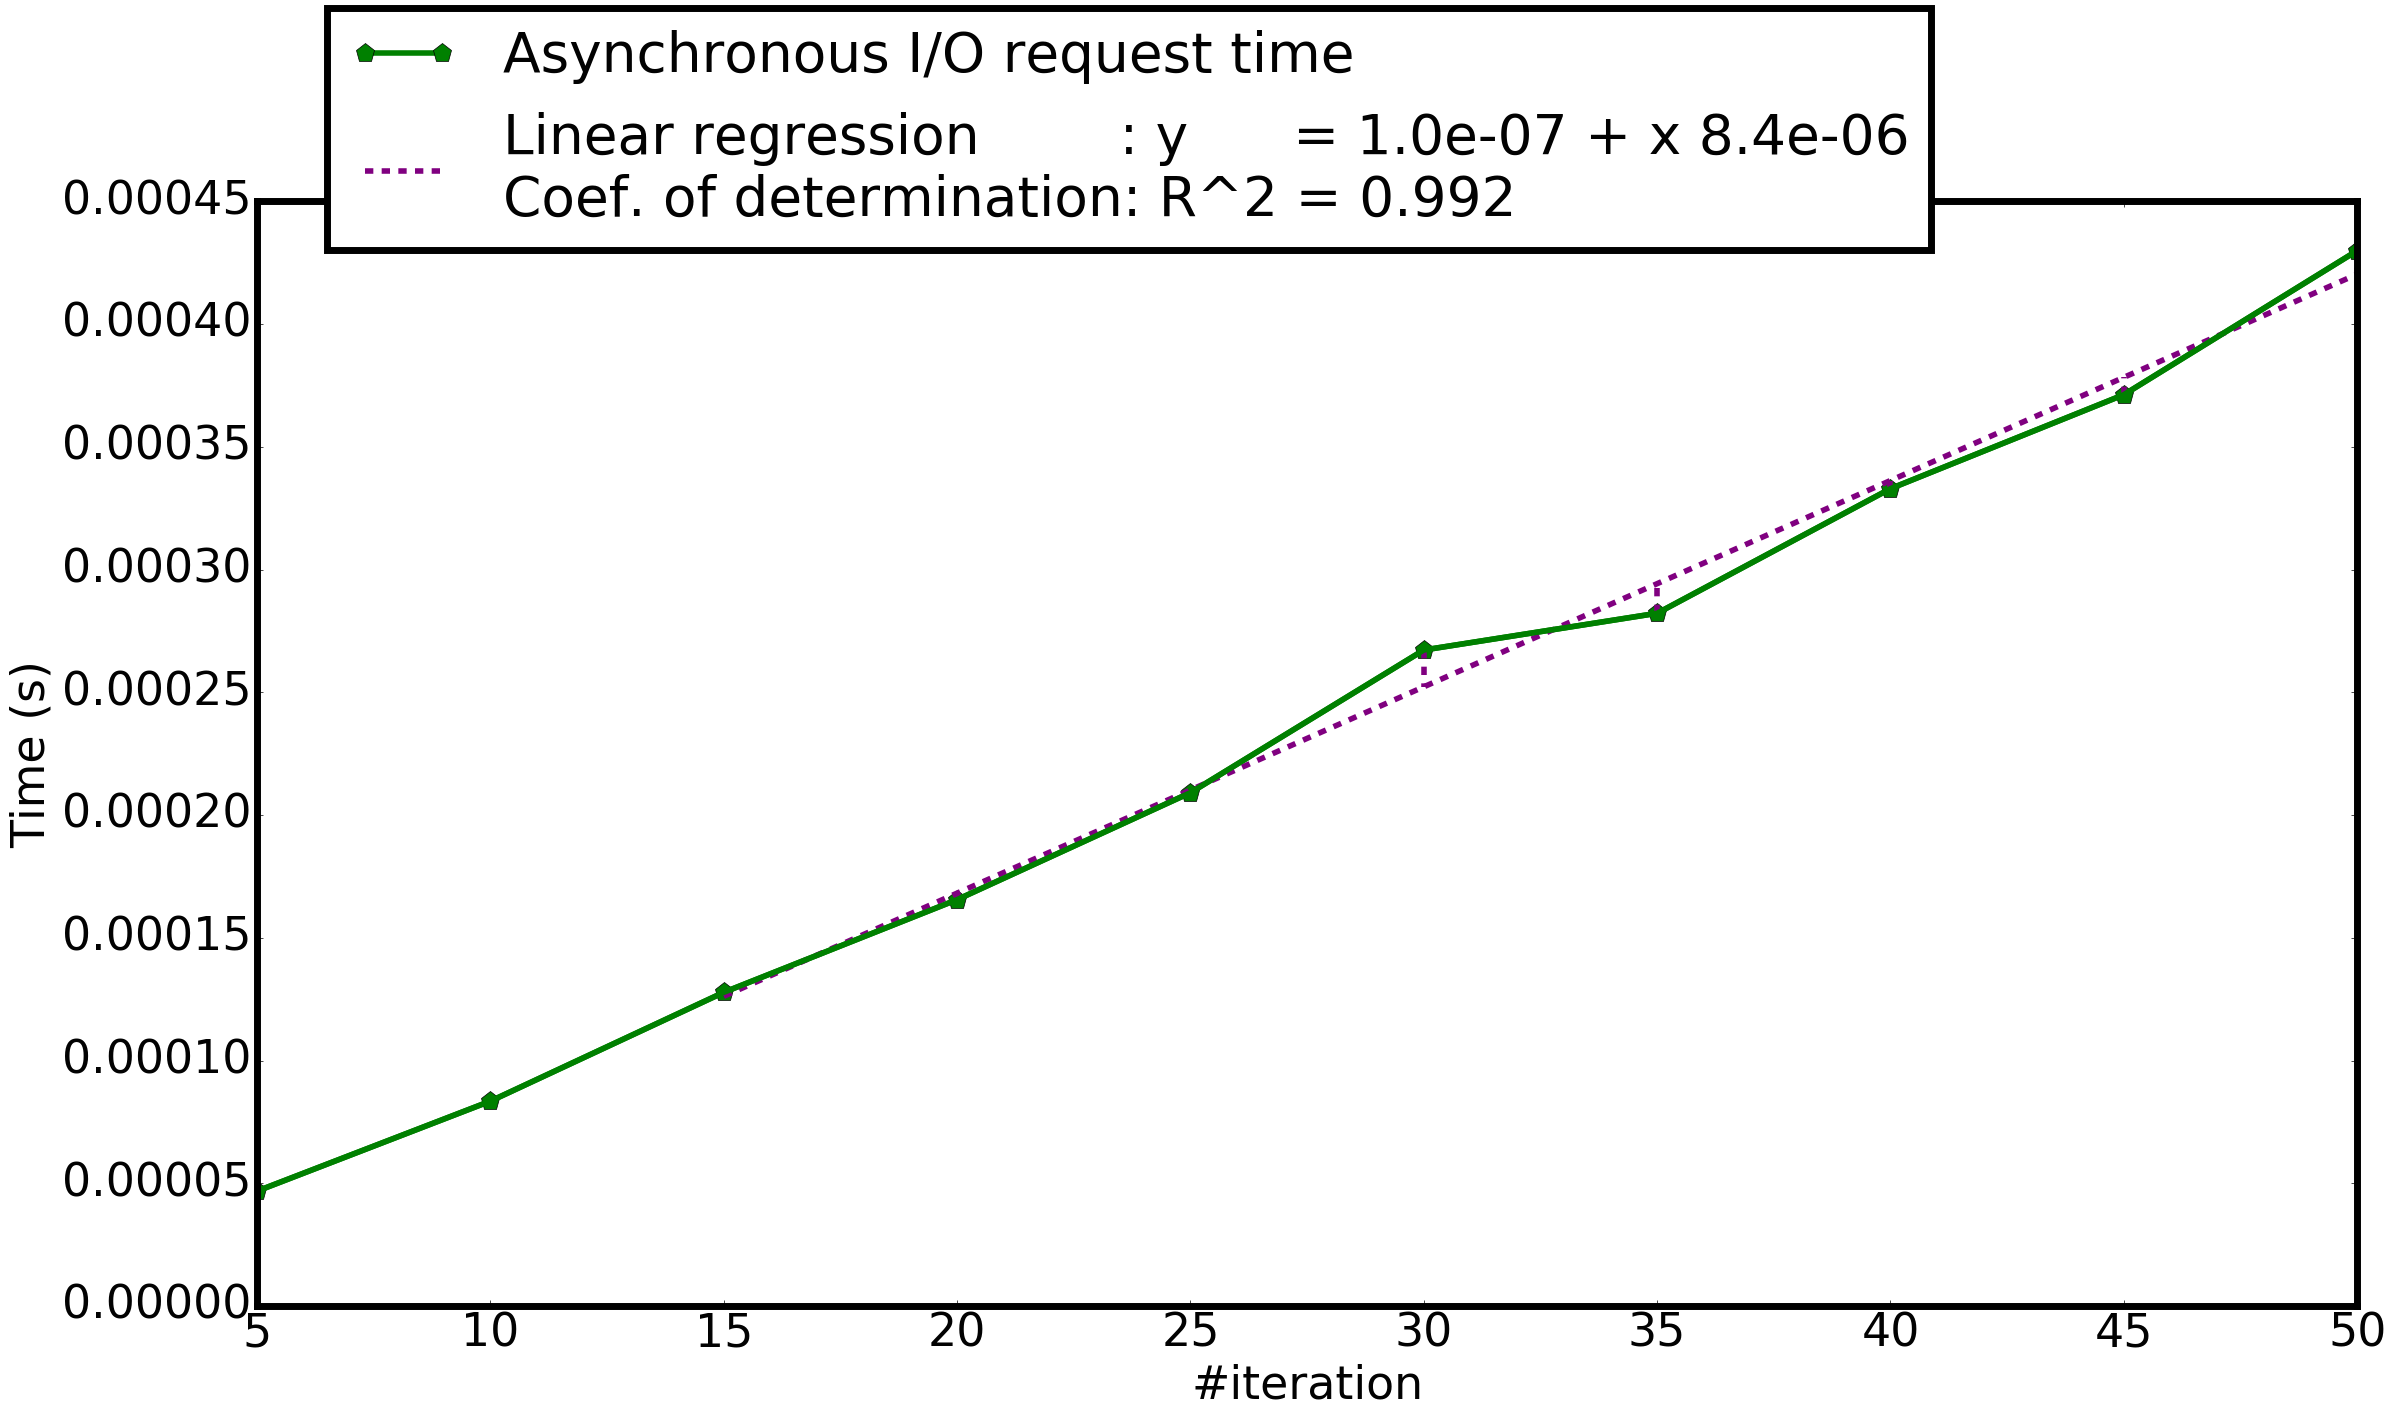
\includegraphics[width=\textwidth]{charts/requestTimeExample_workstation_8core.png}
						\caption[\targetPlatformLaptop\space @ \targetPlatformLaptopFrequency]
						{{\small \targetPlatformLaptop\space @ \targetPlatformLaptopFrequency}}
					\end{subfigure}
					\hfill
					\begin{subfigure}[b]{0.475\textwidth}  
						\centering 
						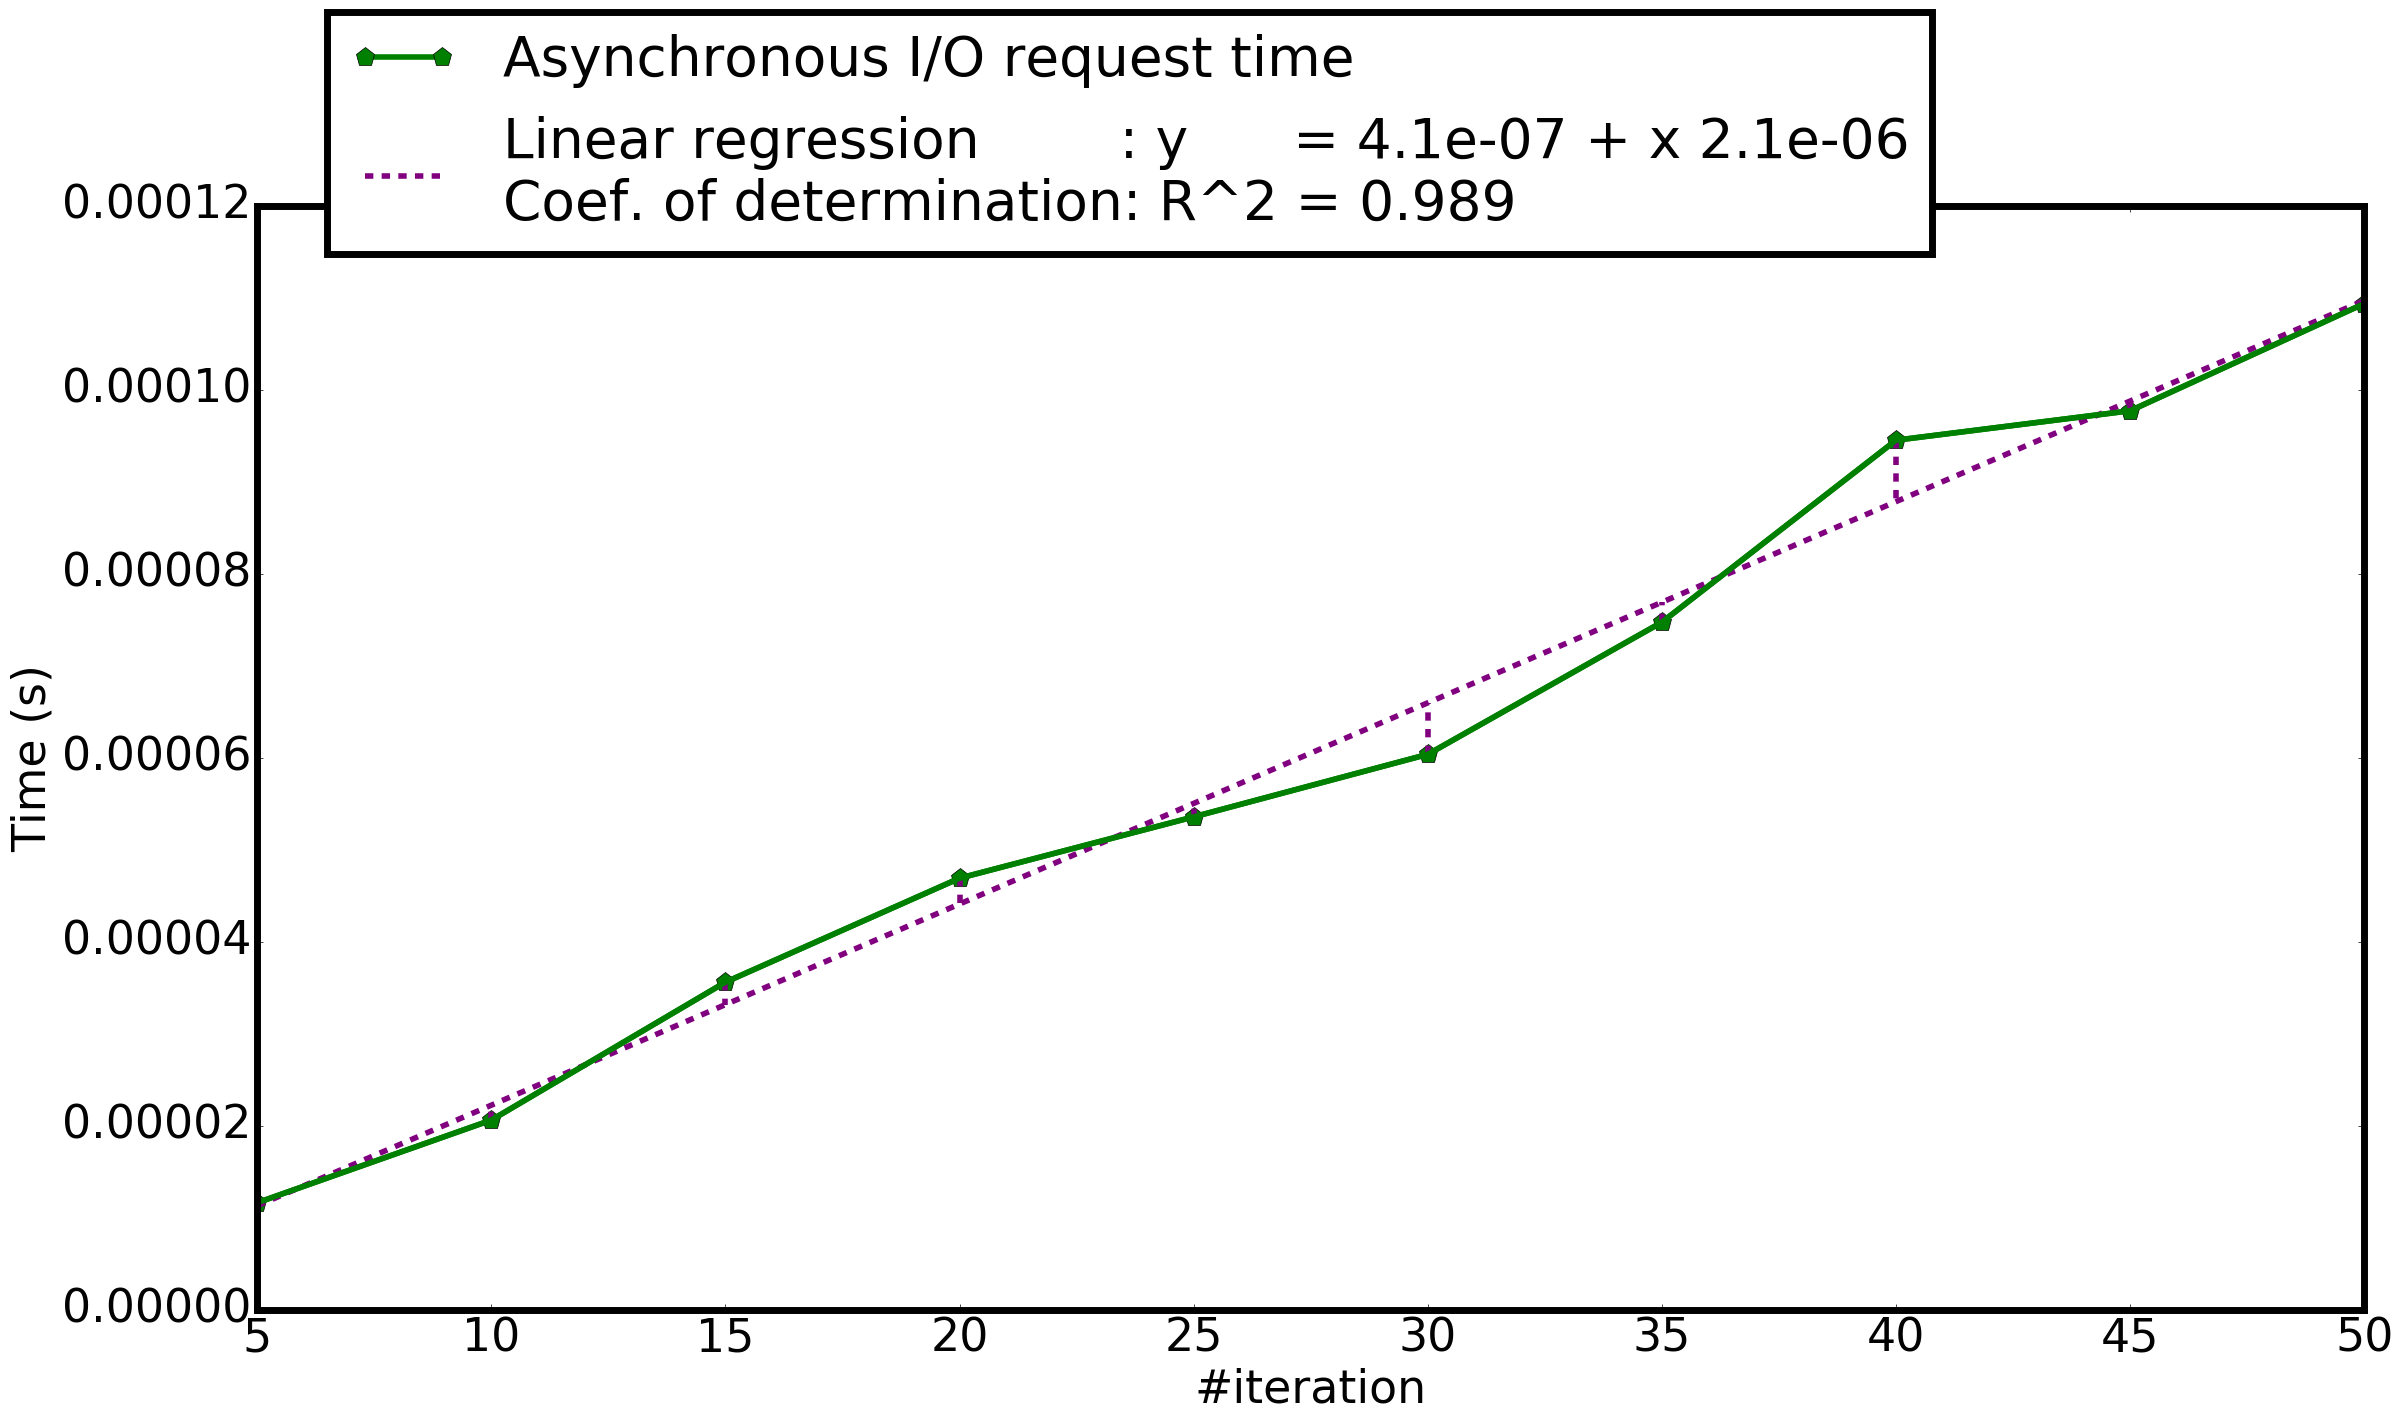
\includegraphics[width=\textwidth]{charts/requestTimeExample_hpc.png}
						\caption[]%
						{{\small \targetPlatformHpc\space @ \targetPlatformHpcFrequency}}    
					\end{subfigure}
					\caption{Experimental assessment of the time for forwarding a request to the asynchronous \notationaioWriteThread}
					\label{fig:requestTimeExample}
				\end{figure*}

			In Figure \ref{fig:requestTimeExample}, we present our experimental evaluation of the \notationaio\space request time ($req$) within the two considered hardware platforms.   Using the numerical method described in Section \ref{subsubsection:modelRequestTime}, we estimate the value of the request time as well as the validity of the hypothesis: constant request time (for a given hardware platform).

			The value of $req$ is the slop of the linear regression (Figure \ref{fig:requestTimeExample}).   This value is, respectively, $8.4 e^{-6}$ seconds and $2.1 e^{-6}$ seconds for the \targetPlatformLaptop\space and the \targetPlatformHpc\space platform.   Moreover, the \emph{coefficient of determination} ($R^{2}=0.992$ and $R^{2}=0.989$) do not contradict our hypothesis about the constancy of the \notationaio\space request time.



%--------------------------------------------
\section{Real-life experimental case: the \toolTargetSoftware}\label{section:experimentalCase}
	Let us now see how the previously presented results may be transposed to a real-life example: the \toolTargetSoftware.\\
	The objective of this section is to check whether the previously noticed improvements brought by our asynchronous \emph{write} implementation may still be achieved within a real-life application.   We also aim to identify any additional perturbation that our \notationaio\space solution may introduce on a general-purpose computation.    In a second step, we evaluate our custom solutions to eliminate (or at least to reduce) these undesirable interferences.\\

	All the presented experimental results are obtained following the same protocol.   Each considered point is assessed (experimental run) 10 times in a row.   The presented corresponding value is the average of the result of these 10 runs.   We also present an error bar showing the distance between the maximal and minimal value of these 10 runs.\\
	It is also worthwhile to mention that for all the following experimentations, the used inputs\footnote{Performance profile file (see Section \ref{section:workingFramework})} of the \toolTargetSoftware\space have not been processed nor modified.   Thus, the observed executions of the \toolTargetSoftware\space are performed in a real-life conditions and with real-life data samples.\\
	All the used input data samples (performance profiling file) have been obtained by profiling the execution of the \emph{NAS parallel benchmark}\footnote{Set of programs designed by \emph{NASA} to help evaluate the performance of parallel supercomputers. The benchmarks are derived from computational fluid dynamics (CFD) applications}.   They all represent the execution of about $10^{5}$ threads.   Each file is about $10^{9}$ Bytes large.


	\subsection{Basic POSIX-based asynchronous implementation}
		In this first step, we embed our basic asynchronous writing strategy within the \toolTargetSoftware.   The experimental assessments of this implementation are compared in Figures \ref{fig:cubeRemapper_basicImplementation_write} and \ref{fig:cubeRemapper_basicImplementation_compute_total} to the state-of-the-art (synchronous) implementation of the \toolTargetSoftware\space.\\

			\begin{figure*}[!h]
				\centering
				\begin{subfigure}[b]{0.475\textwidth}
					\centering
					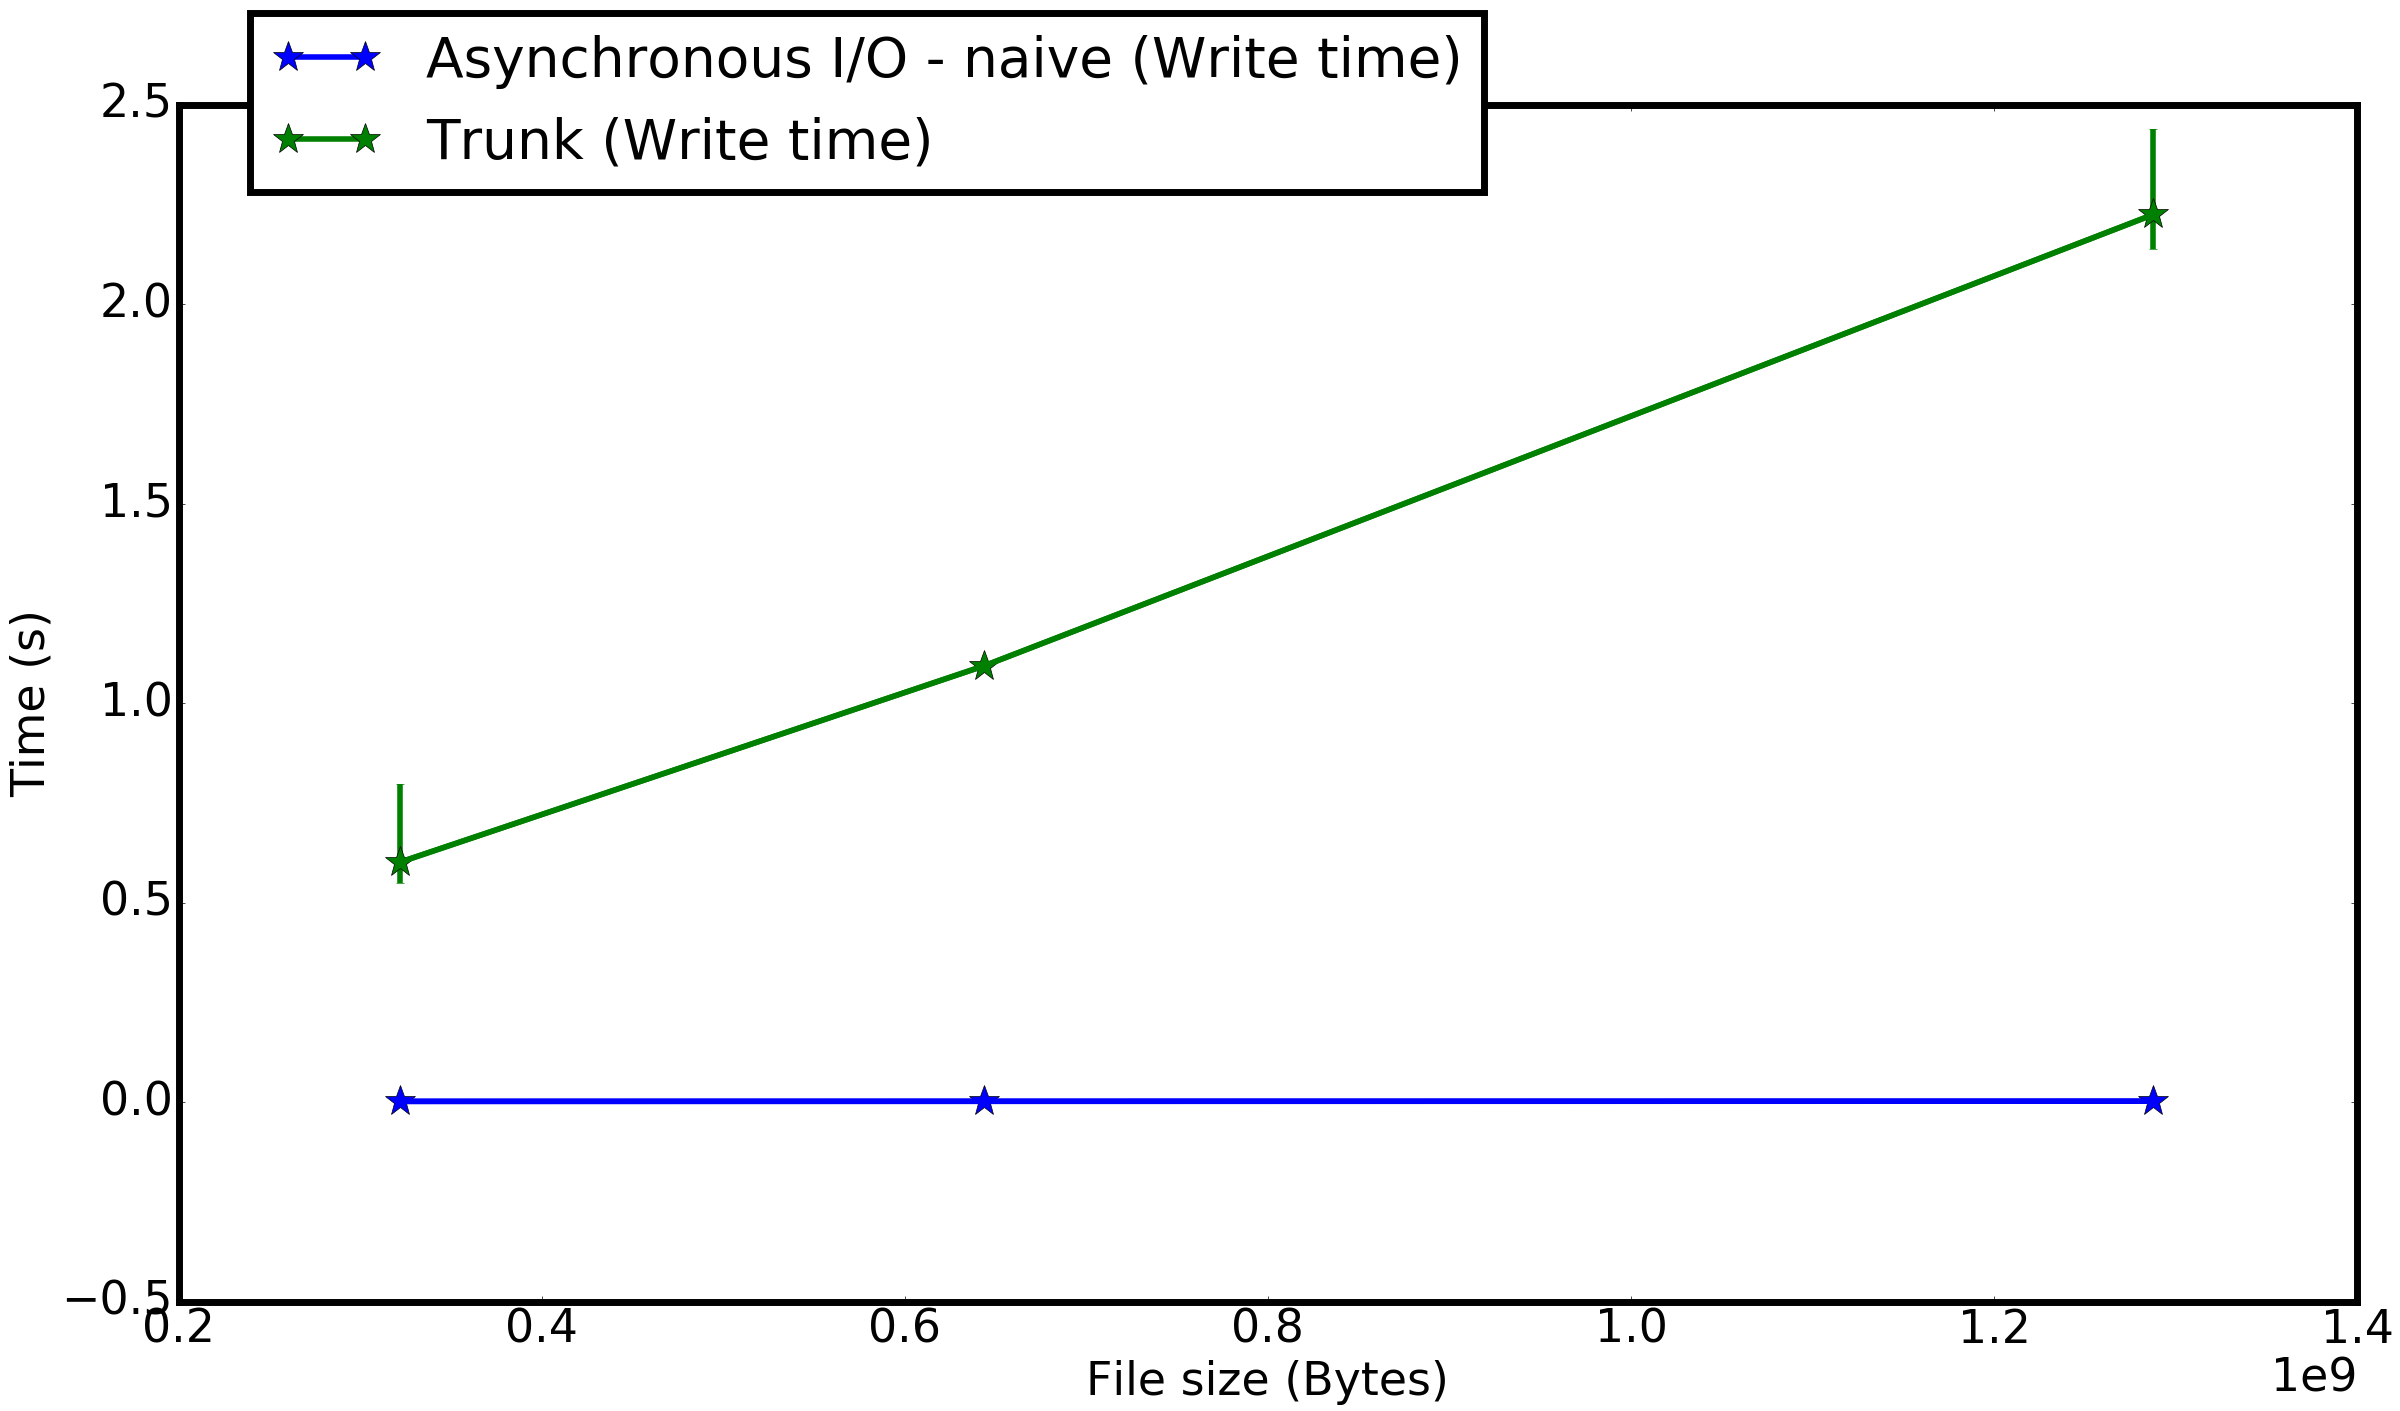
\includegraphics[width=\textwidth]{charts/cubeRemapper_basicImplementation_write_workstation_8core.png}
					\caption[\targetPlatformLaptop \space @ \targetPlatformLaptopFrequency]
					{{\small \targetPlatformLaptop \space @ \targetPlatformLaptopFrequency}}
				\end{subfigure}
				\hfill
				\begin{subfigure}[b]{0.475\textwidth}
					\centering
					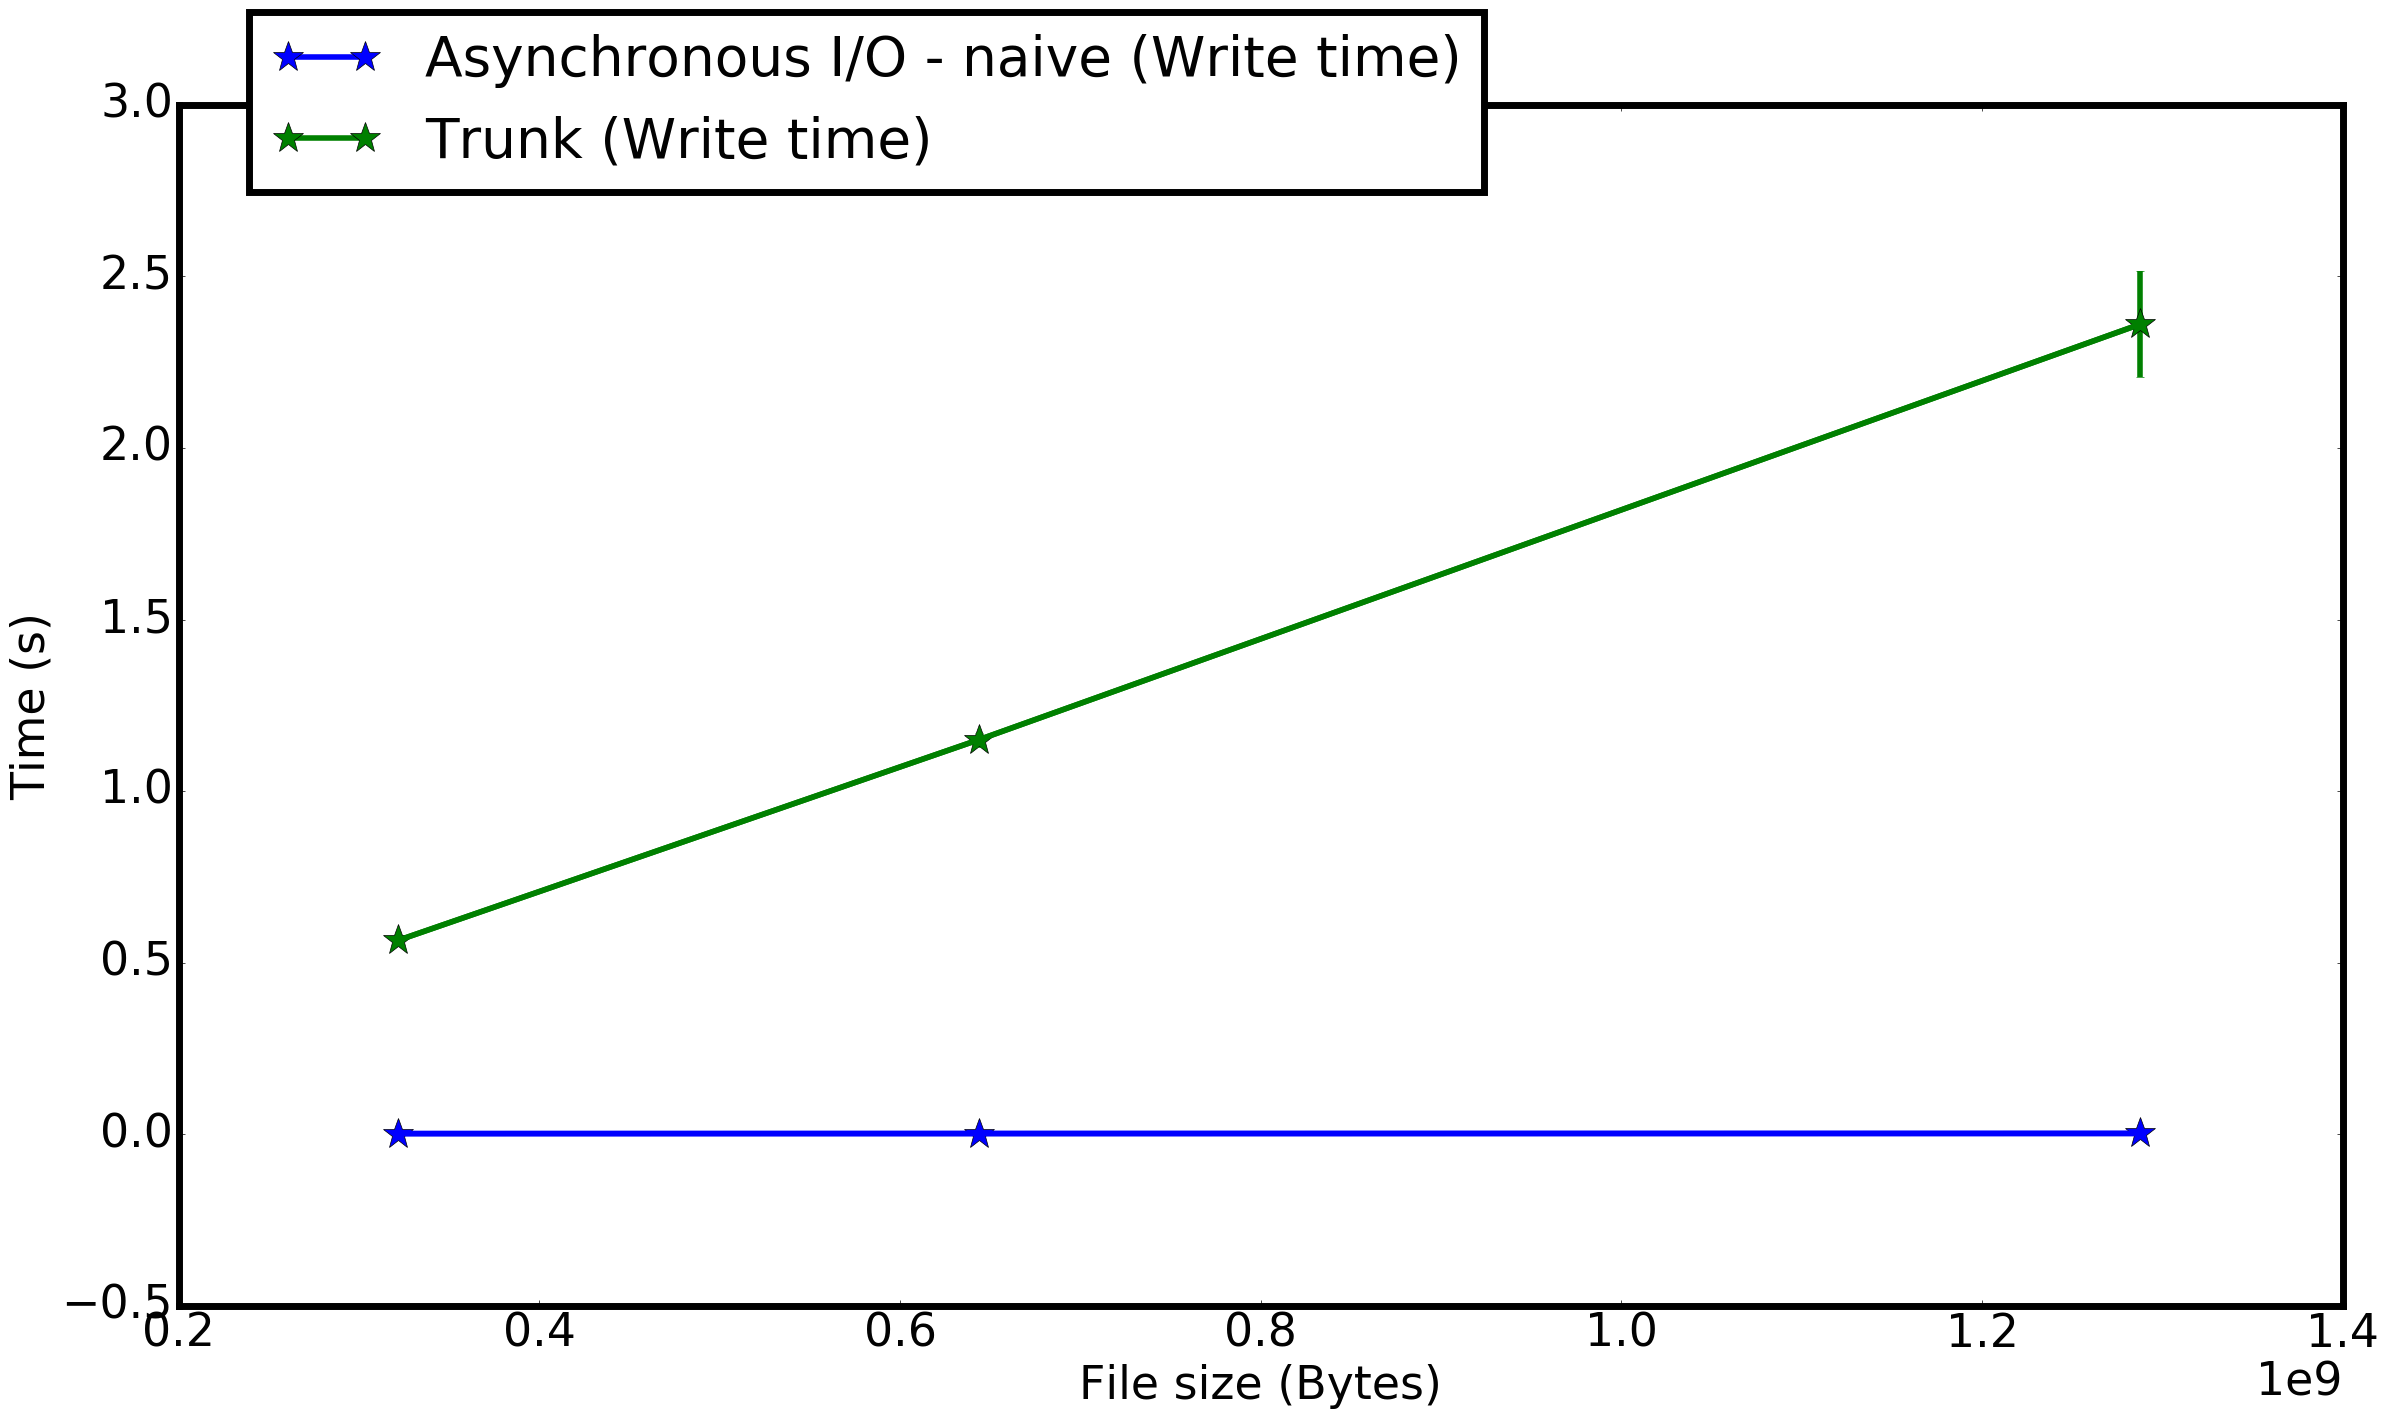
\includegraphics[width=\textwidth]{charts/cubeRemapper_basicImplementation_write_hpc.png}
					\caption[]%
					{{\small \targetPlatformHpc \space @ \targetPlatformHpcFrequency}}
				\end{subfigure}
				\caption{Experimental comparison of the \emph{write} time: proposed \emph{\notationaio\space} (naive) VS. \emph{state-of-the-art} (trunk synchronous) implementation of the \toolTargetSoftware}
				\label{fig:cubeRemapper_basicImplementation_write}
			\end{figure*}

		As one could expect, Figure \ref{fig:cubeRemapper_basicImplementation_write} shows that the \emph{write} time of our custom basic implementation is now almost null (compared to the synchronous \emph{write} time).   Instead of waiting for a costly \notationIO\space \emph{write} time at each iteration, we simply wait for the time to enqueue a request within a shared queue.   Given the reduced \emph{write} time (compared to the \emph{compute} time), the \notationaio\space strategy has a negligible final waiting\footnote{Time to wait for the pending \notationaio\space request to be executed once all the \emph{compute} operations have been executed} time.\\

			\begin{figure*}[!h]
				\centering
				\begin{subfigure}[b]{0.475\textwidth}
					\centering
					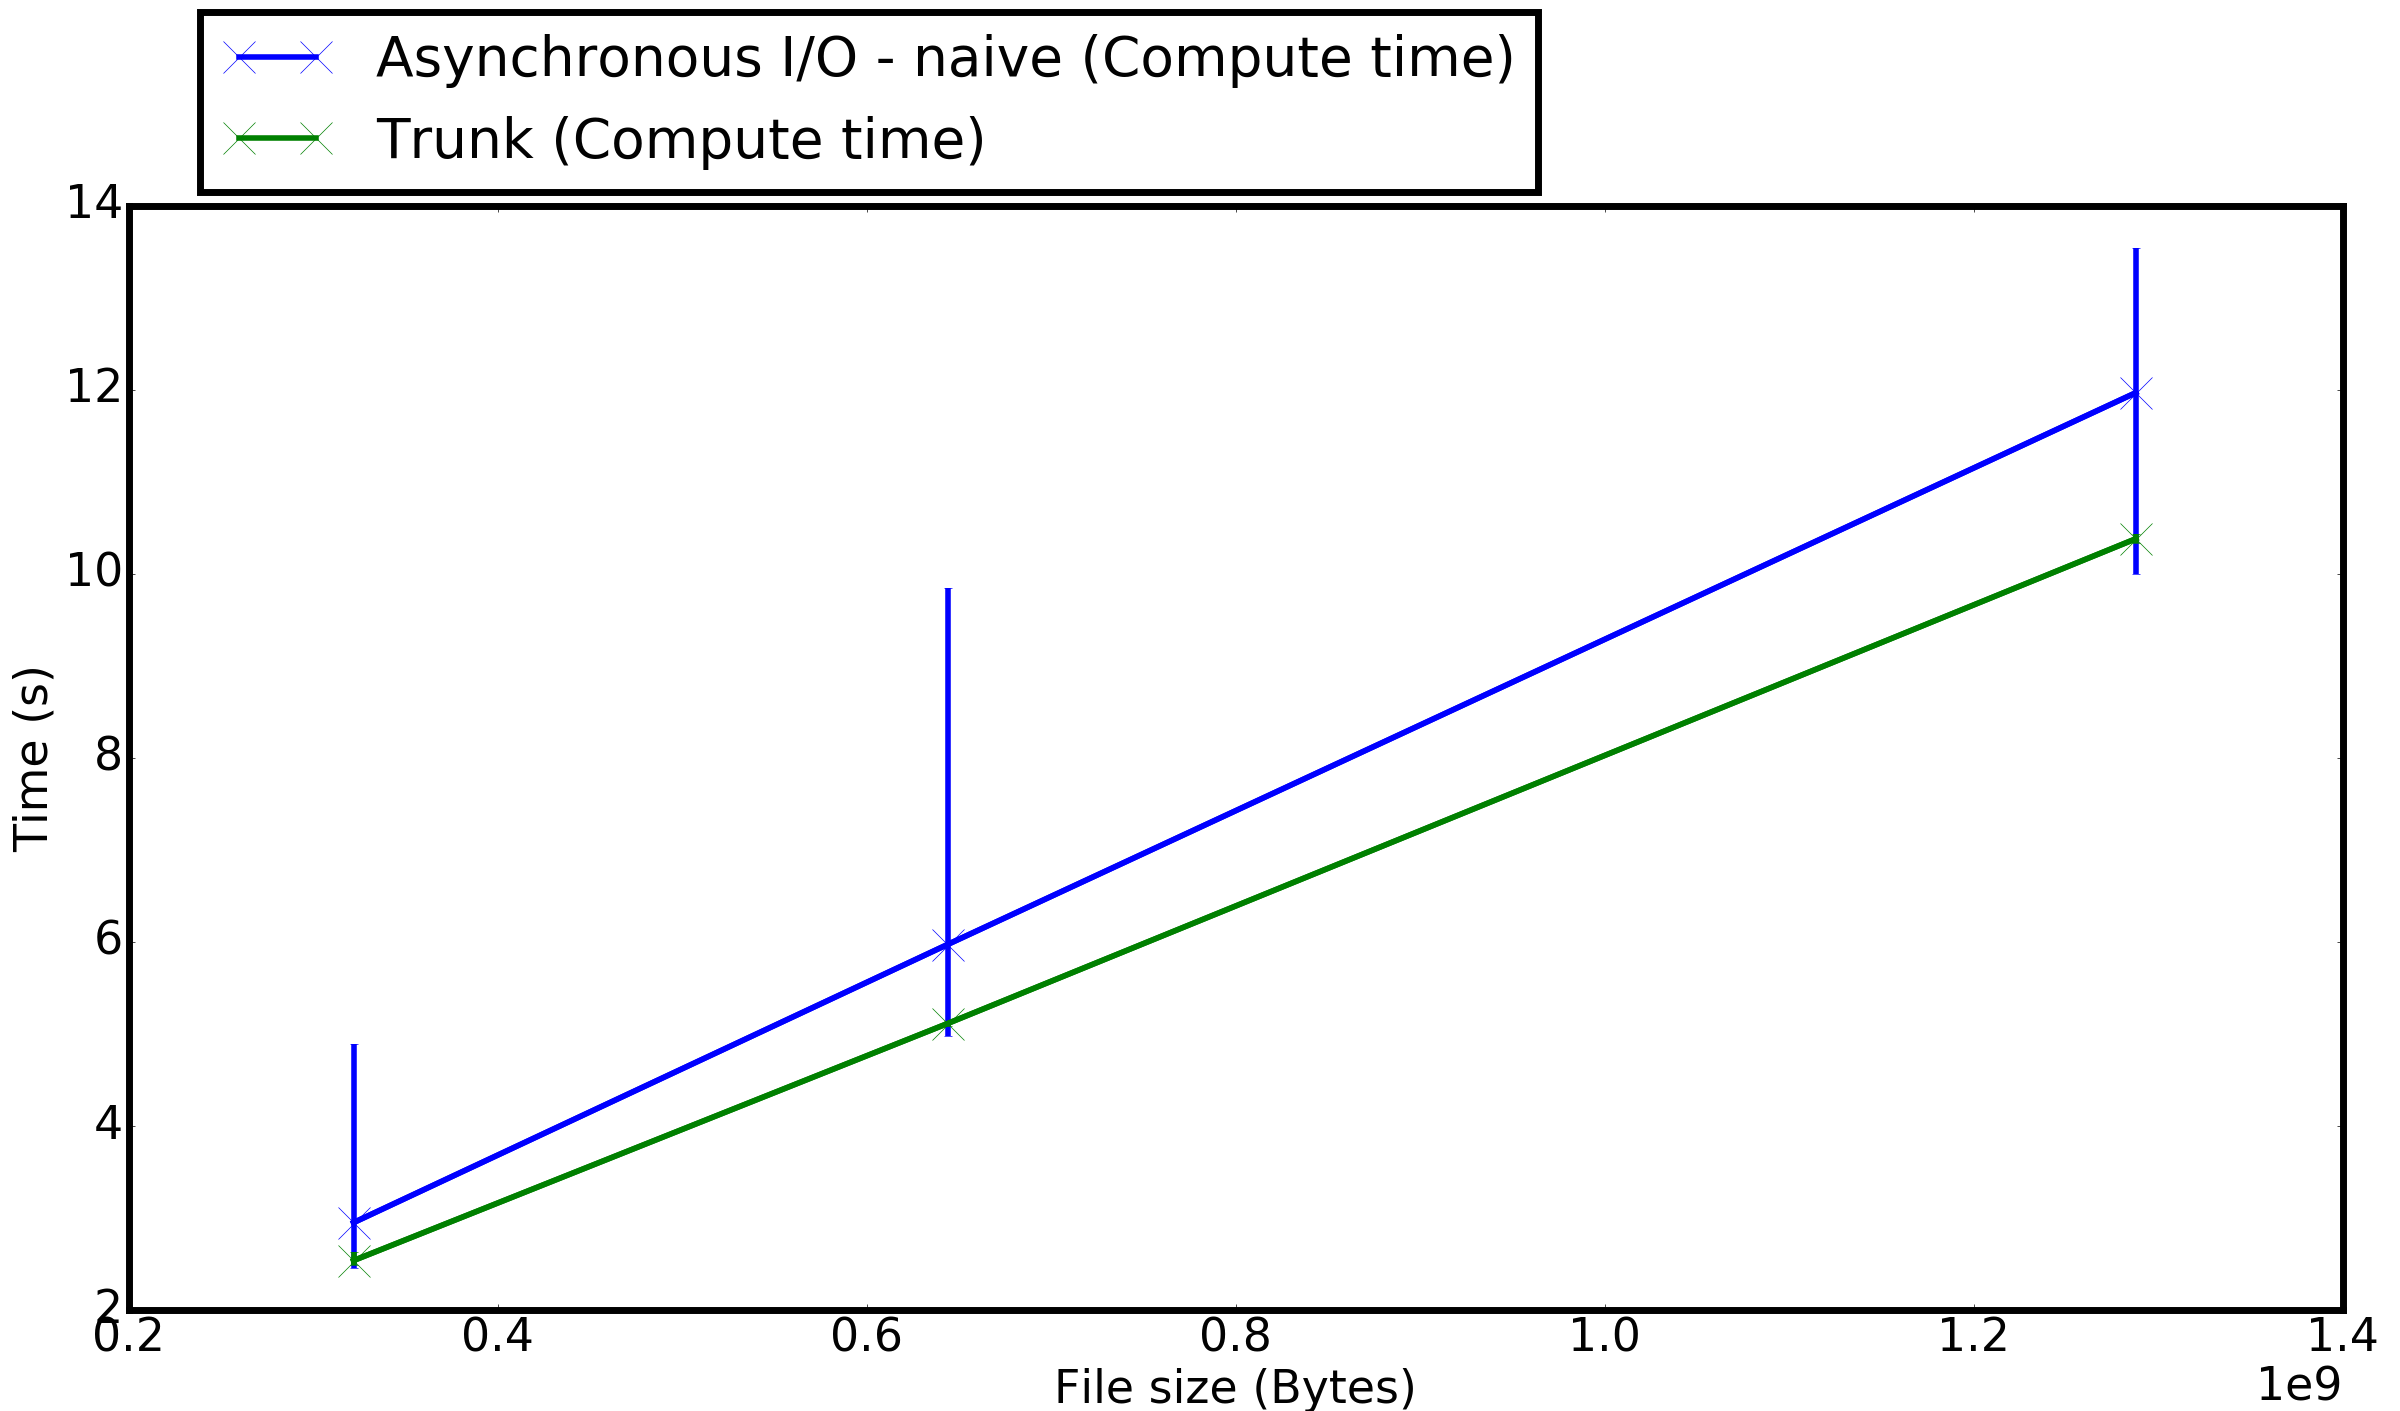
\includegraphics[width=\textwidth]{charts/cubeRemapper_basicImplementation_compute_workstation_8core.png}
					\caption[\targetPlatformLaptop \space @ \targetPlatformLaptopFrequency]
					{{\small \targetPlatformLaptop \space @ \targetPlatformLaptopFrequency}}
					\label{fig:cubeRemapper_basicImplementation_compute_workstation_8core}
				\end{subfigure}
				\hfill
				\begin{subfigure}[b]{0.475\textwidth}
					\centering
					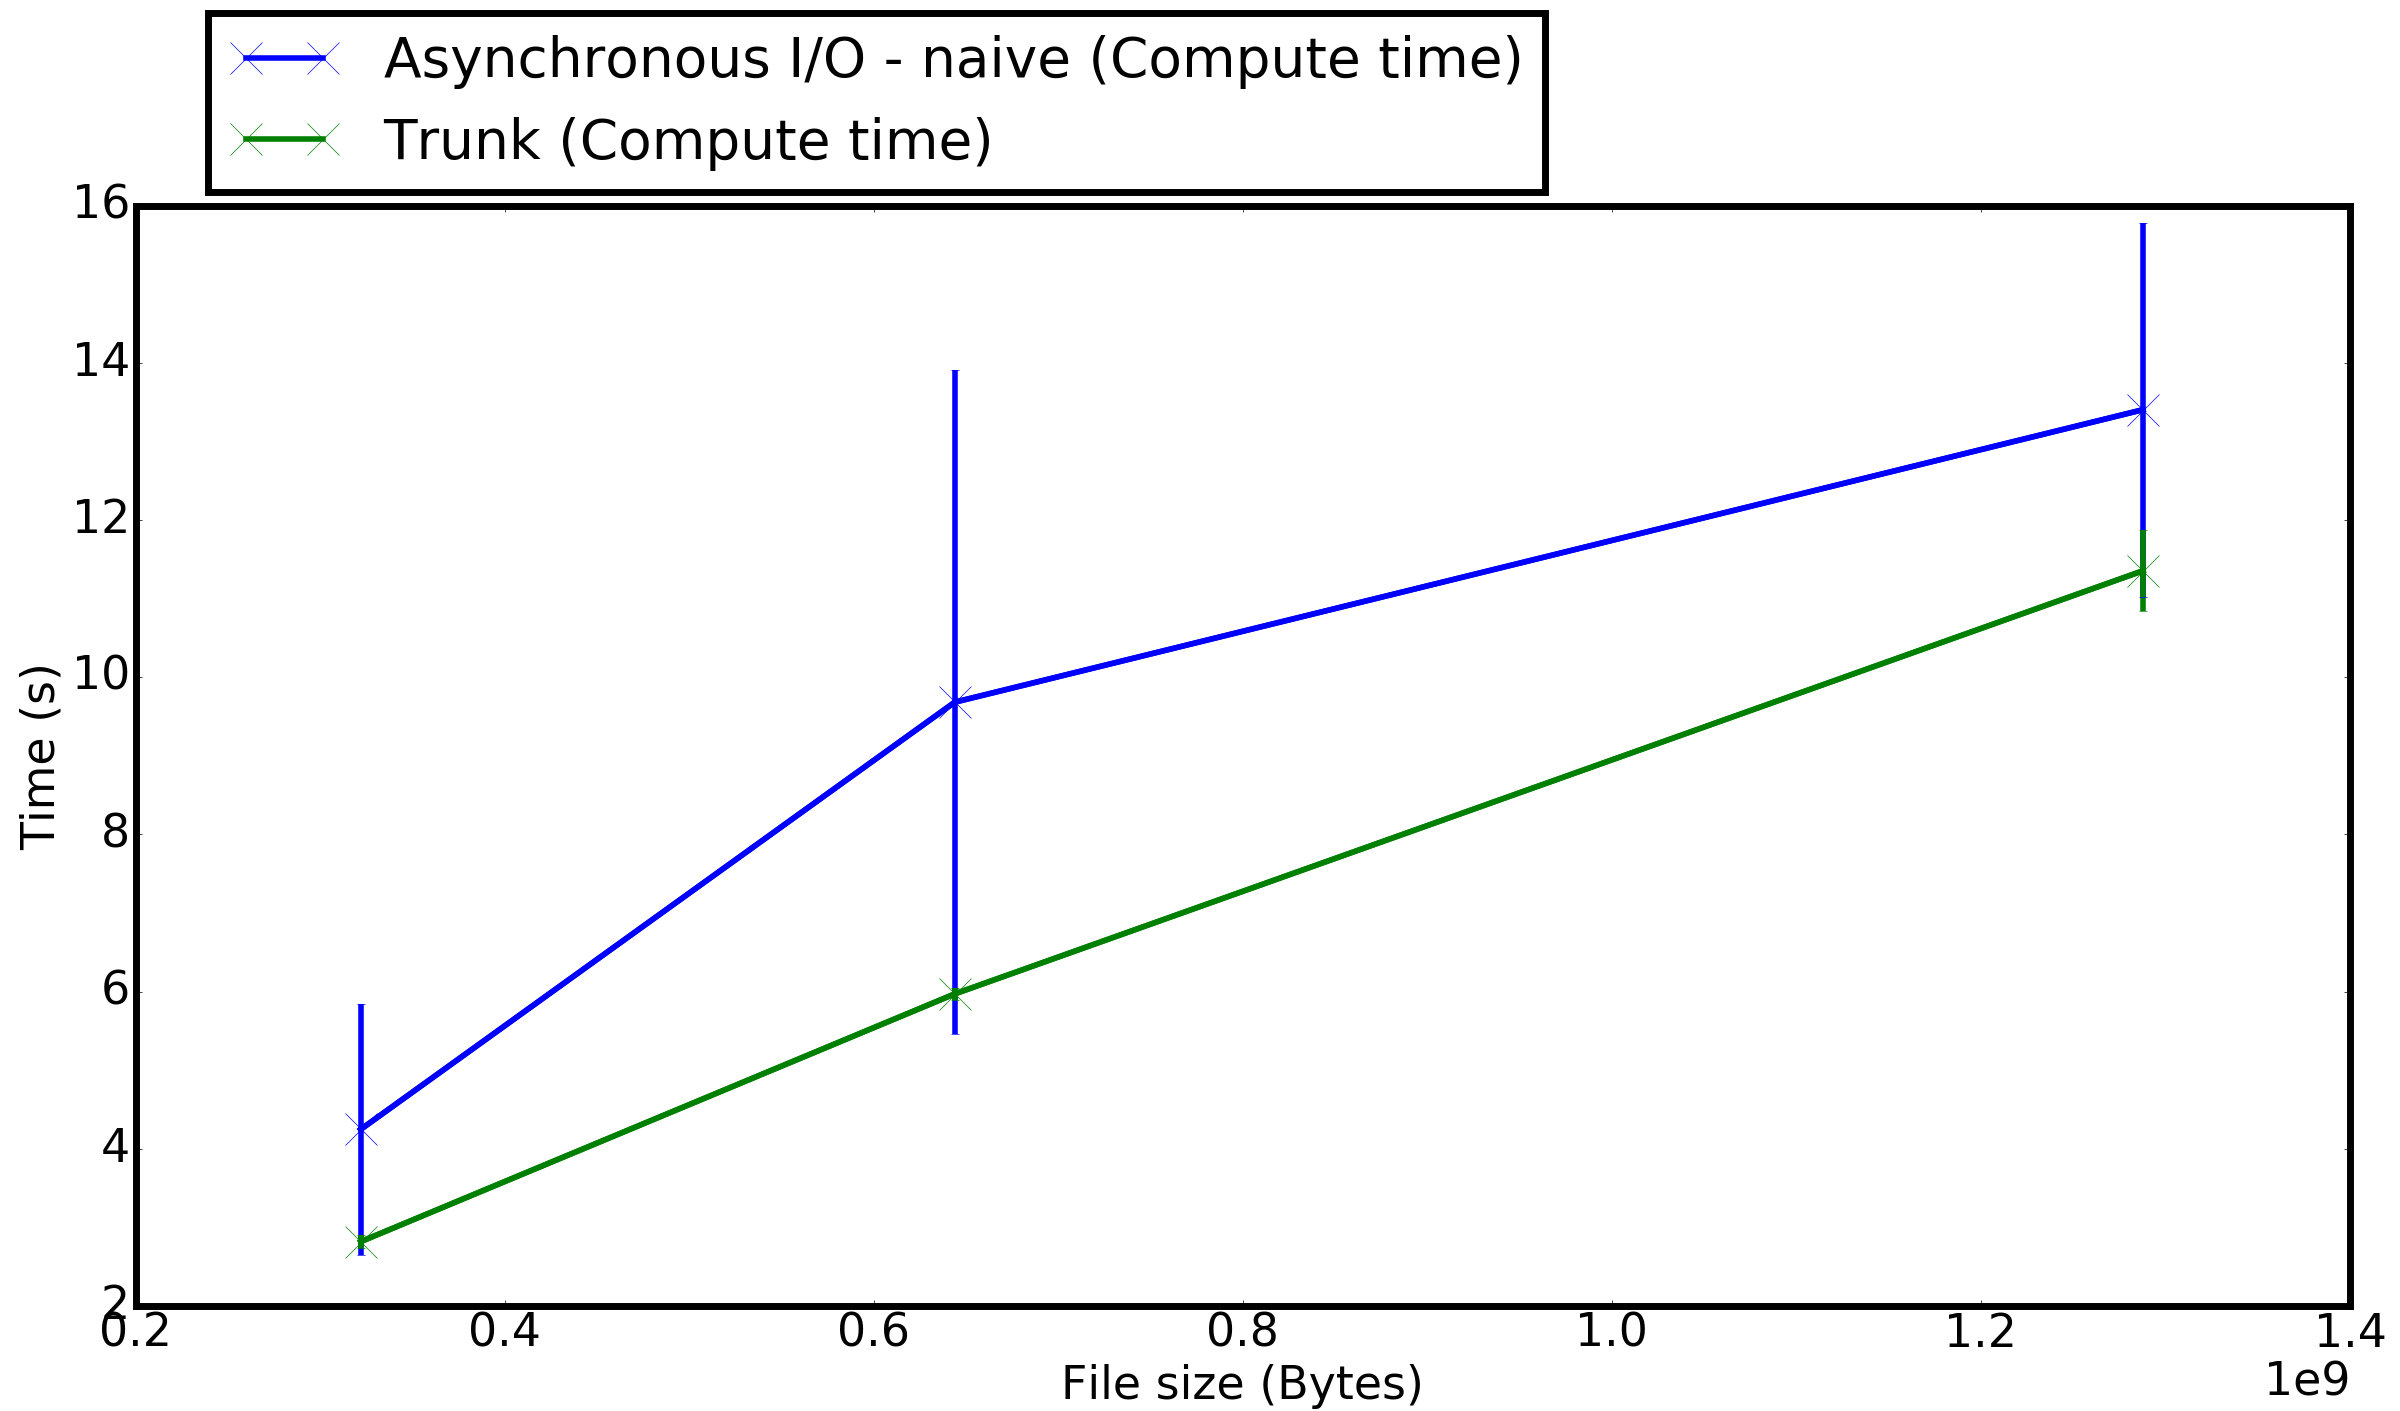
\includegraphics[width=\textwidth]{charts/cubeRemapper_basicImplementation_compute_hpc.png}
					\caption[]%
					{{\small \targetPlatformHpc \space @ \targetPlatformHpcFrequency}}    
					\label{fig:cubeRemapper_basicImplementation_compute_hpc}
				\end{subfigure}
				\hfill
				\begin{subfigure}[b]{0.475\textwidth}
					\centering
					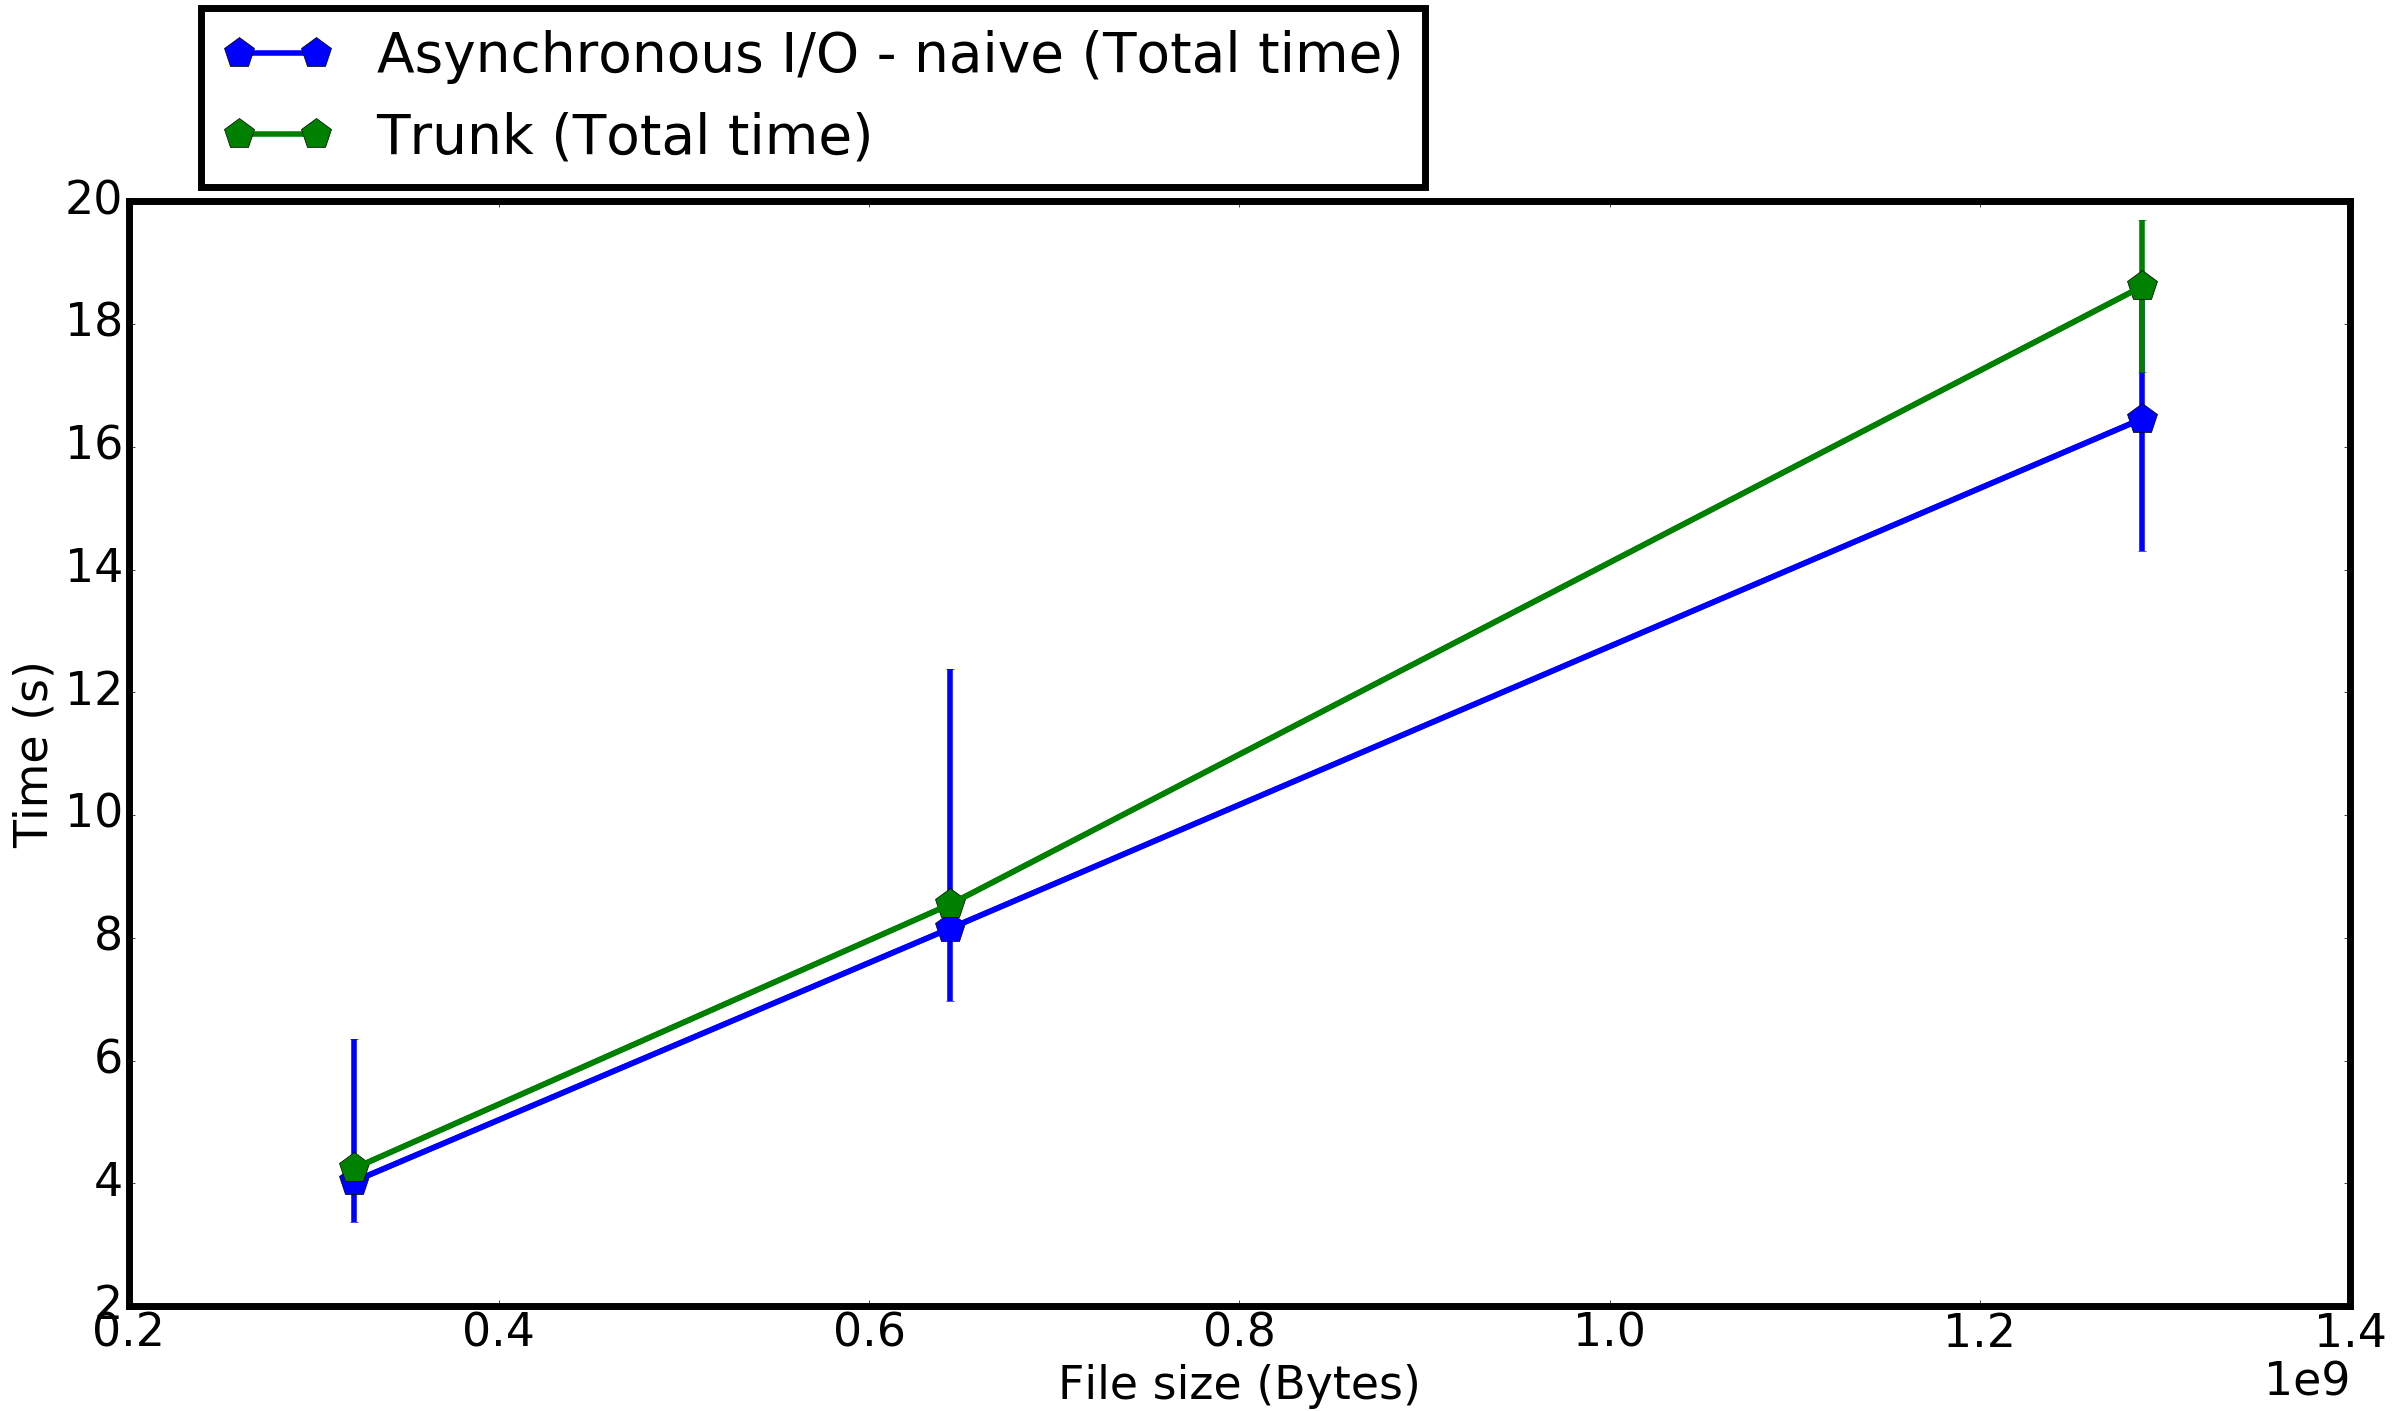
\includegraphics[width=\textwidth]{charts/cubeRemapper_basicImplementation_total_workstation_8core.png}
					\caption[\targetPlatformLaptop \space @ \targetPlatformLaptopFrequency]
					{{\small \targetPlatformLaptop \space @ \targetPlatformLaptopFrequency}}
					\label{fig:cubeRemapper_basicImplementation_total_workstation_8core}
				\end{subfigure}
				\hfill
				\begin{subfigure}[b]{0.475\textwidth}
					\centering
					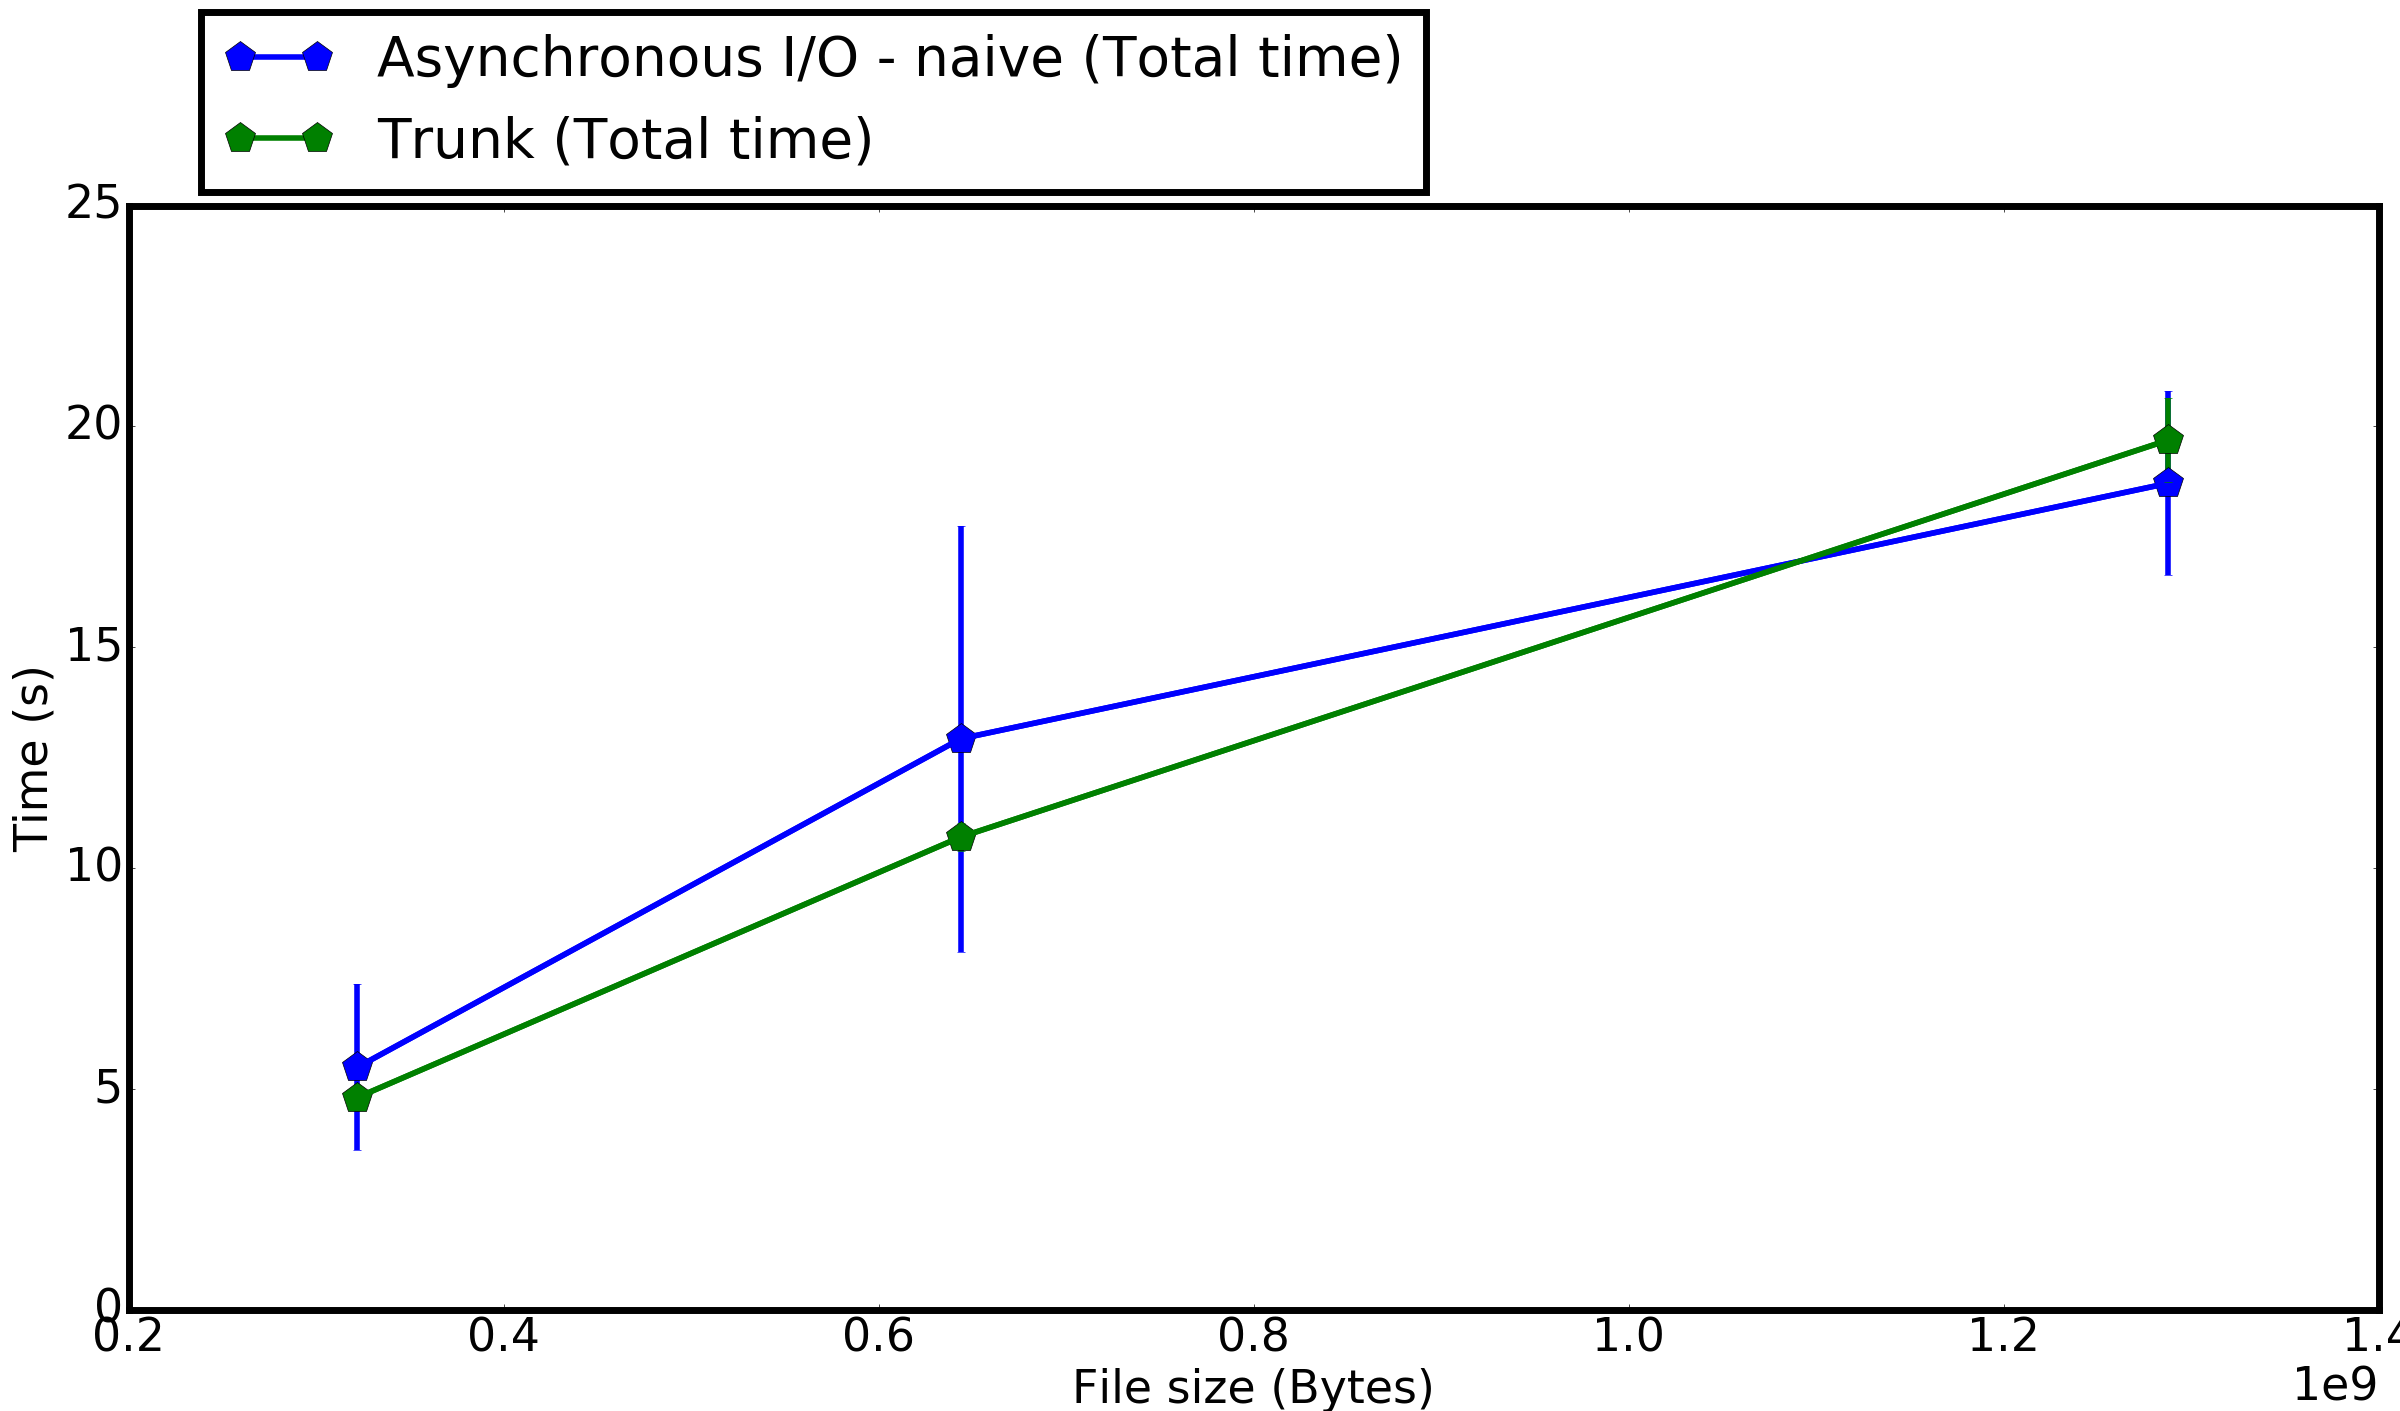
\includegraphics[width=\textwidth]{charts/cubeRemapper_basicImplementation_total_hpc.png}
					\caption[]%
					{{\small \targetPlatformHpc \space @ \targetPlatformHpcFrequency}}    
					\label{fig:cubeRemapper_basicImplementation_total_hpc}
				\end{subfigure}
				\caption{Experimental comparison of the \emph{compute} and \emph{total} time: proposed \emph{\notationaio\space} (naive) VS. \emph{state-of-the-art} (trunk synchronous) implementation of the \toolTargetSoftware}
				\label{fig:cubeRemapper_basicImplementation_compute_total}
			\end{figure*}

		However, the significant performance gain achieved in the \emph{write} operation is not transposed on the total time.   Indeed, Figures \ref{fig:cubeRemapper_basicImplementation_total_workstation_8core} and \ref{fig:cubeRemapper_basicImplementation_total_hpc} show that, on both considered platforms, the overall performance of our custom implementation is roughly comparable to that of the \emph{state-of-the-art}.   The gain achieved in the \emph{write} operation is lost in the \emph{compute} operation\footnote{This performance is shown by Figure \ref{fig:cubeRemapper_basicImplementation_compute_total}}.   More concerning is the \emph{compute} operation in our implementation.   Its value fluctuates within a range from $40$ to $80\%$.   Moreover, although our custom version and the state-of-the-art version use the same \emph{compute} function, we obtain a different response-time when this function is shipped to our implementation of the \toolTargetSoftware.\\


	\subsection{Improving the asynchronous-thread scheduling policy} \label{subsection:improveSchedulingPolicy}
		Based on our previous experimental observations, one could notice the interference between the \emph{compute} operation and our custom \emph{write} implementation.   Indeed, the \emph{compute} operation becomes less efficient once shipped to our version of the \toolTargetSoftware\space (despite the fact that it is the same implementations).\\
		Given the instability of this perturbation (see Figures \ref{fig:cubeRemapper_basicImplementation_compute_workstation_8core} and \ref{fig:cubeRemapper_basicImplementation_compute_hpc}), our first hypothesis to explain this phenomenon is related to the OS-scheduler policy.\\

		As all the considered threads (those processing the \emph{compute} and the \emph{write} operations) belong to the same process, the OS scheduler will tend to run them on the same CPU-core as often as possible (for cache proximity purpose).   Thus, the execution time of the \notationaioComputeThread\space is time-sliced and regularly interrupted for the execution of the \notationaioWriteThreads, most likely on the same CPU-core.   This may explain the delay observed on the experimental assessment of the compute \emph{operation} in our custom implementation (see Figures \ref{fig:cubeRemapper_basicImplementation_compute_workstation_8core} and \ref{fig:cubeRemapper_basicImplementation_compute_hpc}).\\

		Our solution to this resource-multiplexing issue is to pin each running thread on an independent CPU-core.   Assuming that our implementation has a relatively reduced amount of shared data and instructions between these threads (see Section \ref{subsection:dataDistribution}) then, having threads running on independent cores would significantly improve the parallelization with a reduced time overhead\footnote{Minimal shared data is equivalent to minimal synchronization required}.\\
		In order to pin the threads created by the \notationaio\space library, we have used the custom wrapper of the \emph{pthread} library described in Section \ref{subsubsection:pthreadWrapper}.\\

			\begin{figure*}[!h]
				\centering
				\begin{subfigure}[b]{0.475\textwidth}
					\centering
					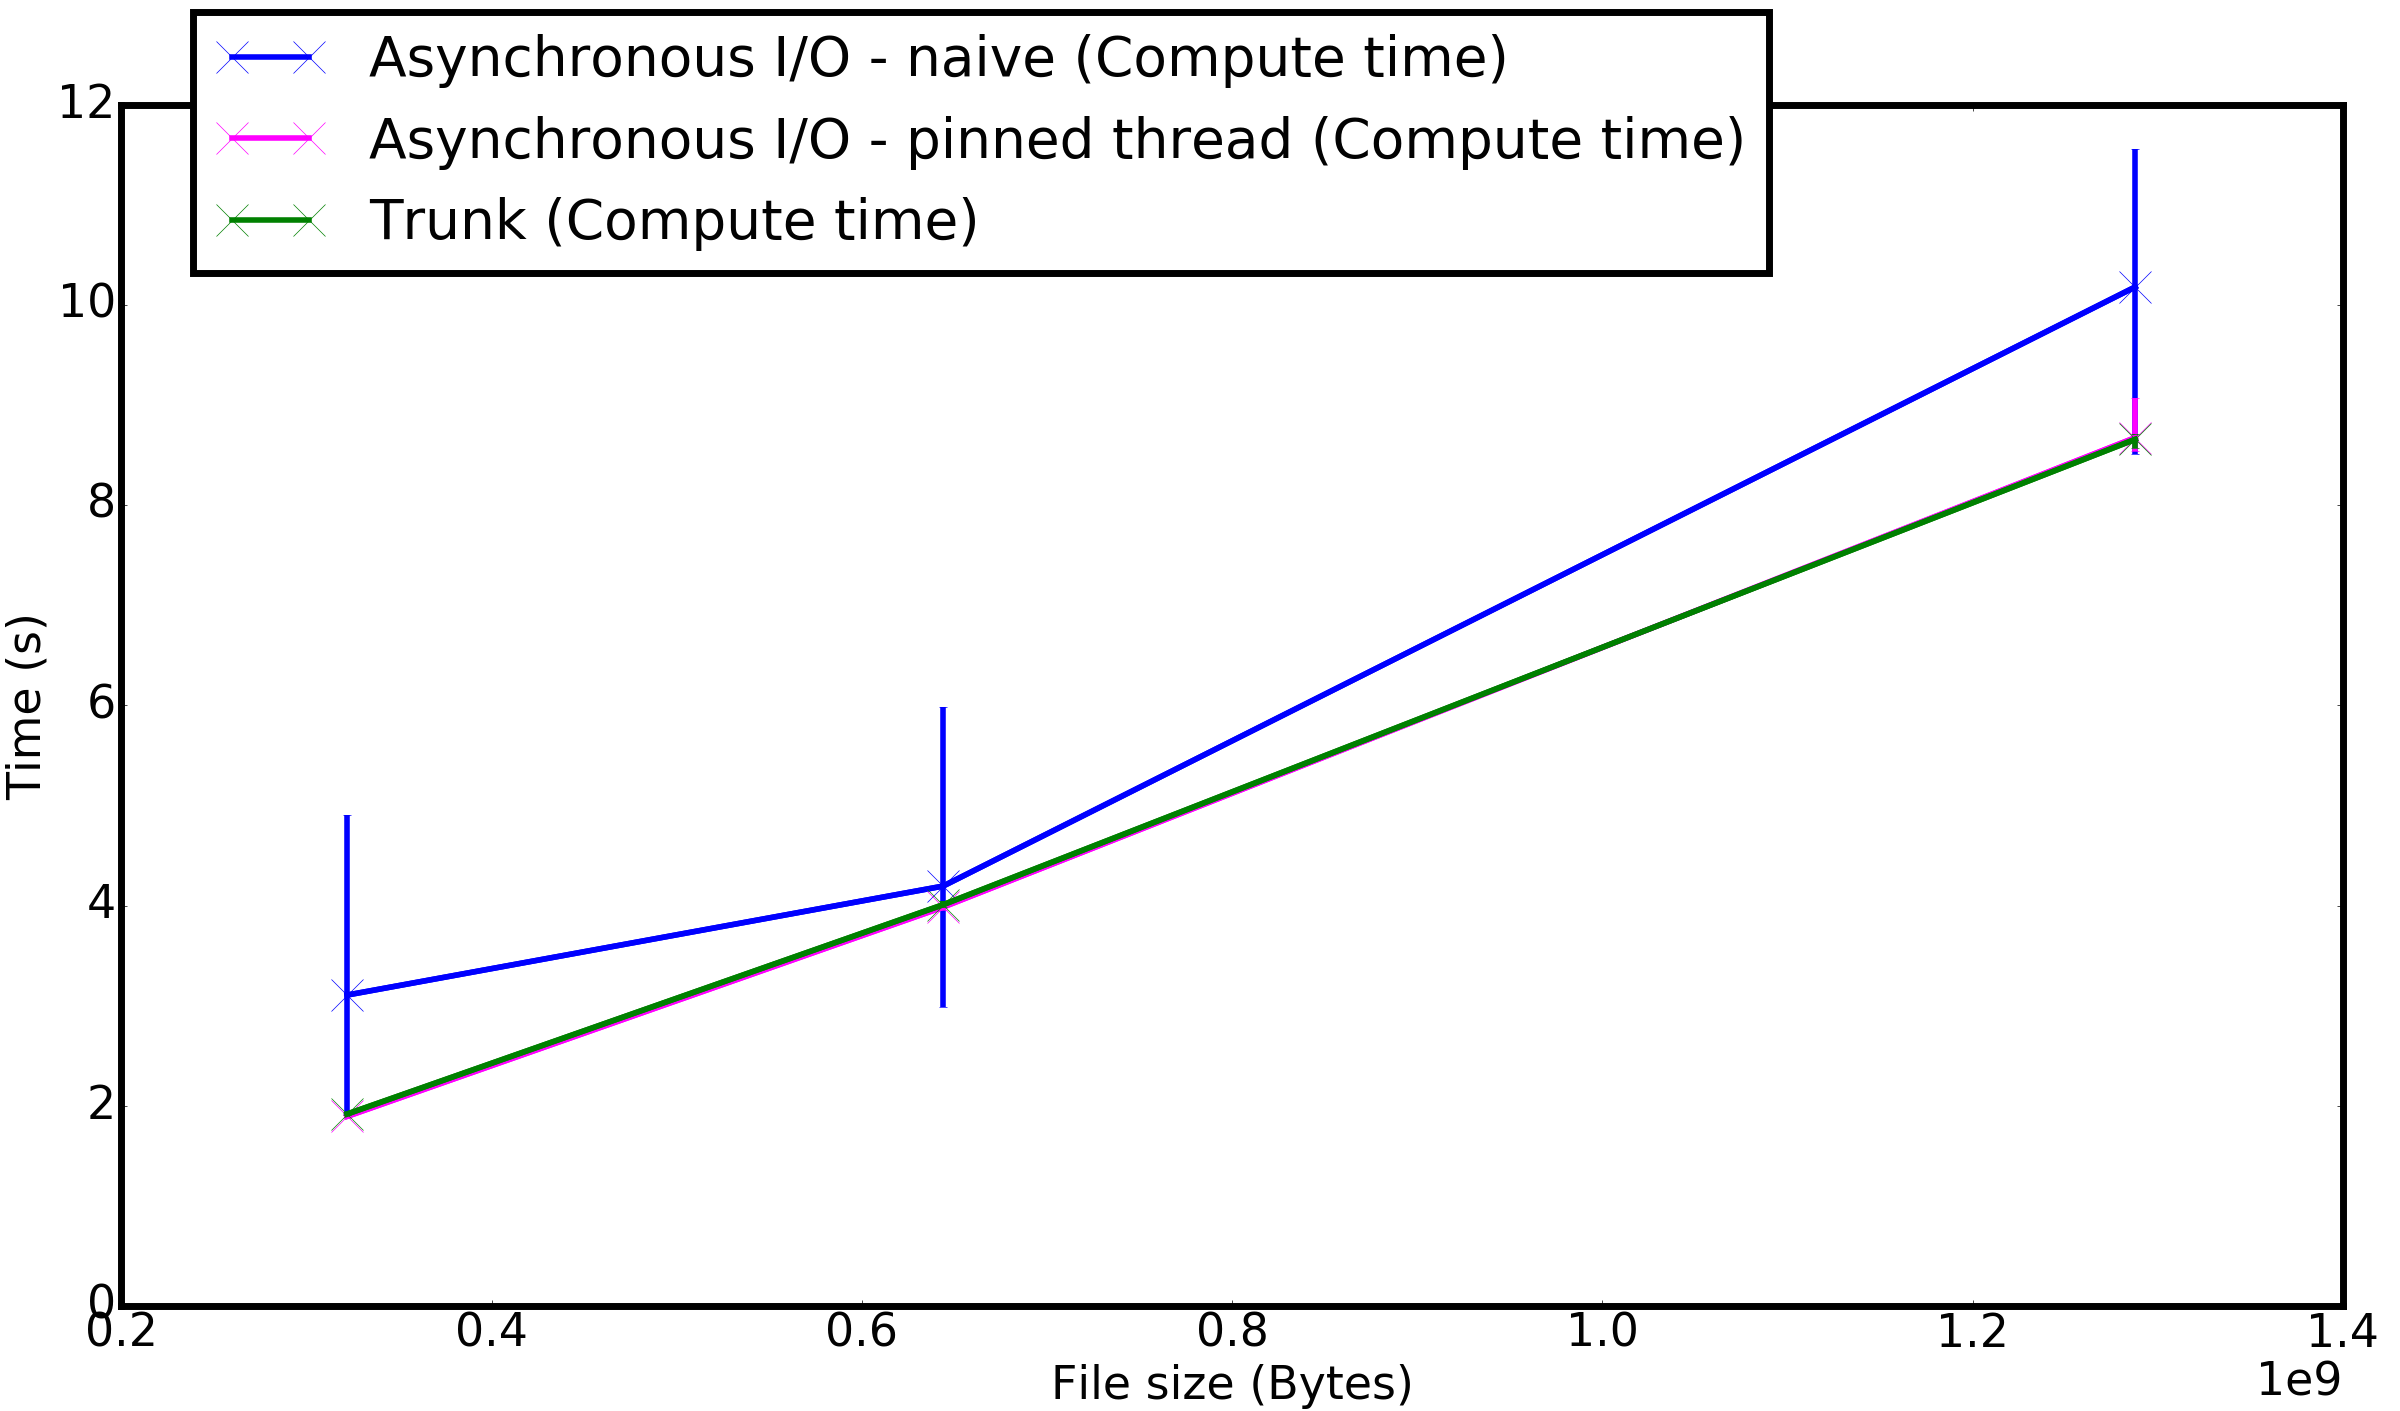
\includegraphics[width=\textwidth]{charts/cubeRemapper_pthreadWrap_compute_workstation_8core.png}
					\caption[\targetPlatformLaptop \space @ \targetPlatformLaptopFrequency]
					{{\small \targetPlatformLaptop \space @ \targetPlatformLaptopFrequency}}
					\label{fig:cubeRemapper_pthreadWrap_compute_workstation}
				\end{subfigure}
				\hfill
				\begin{subfigure}[b]{0.475\textwidth}
					\centering
					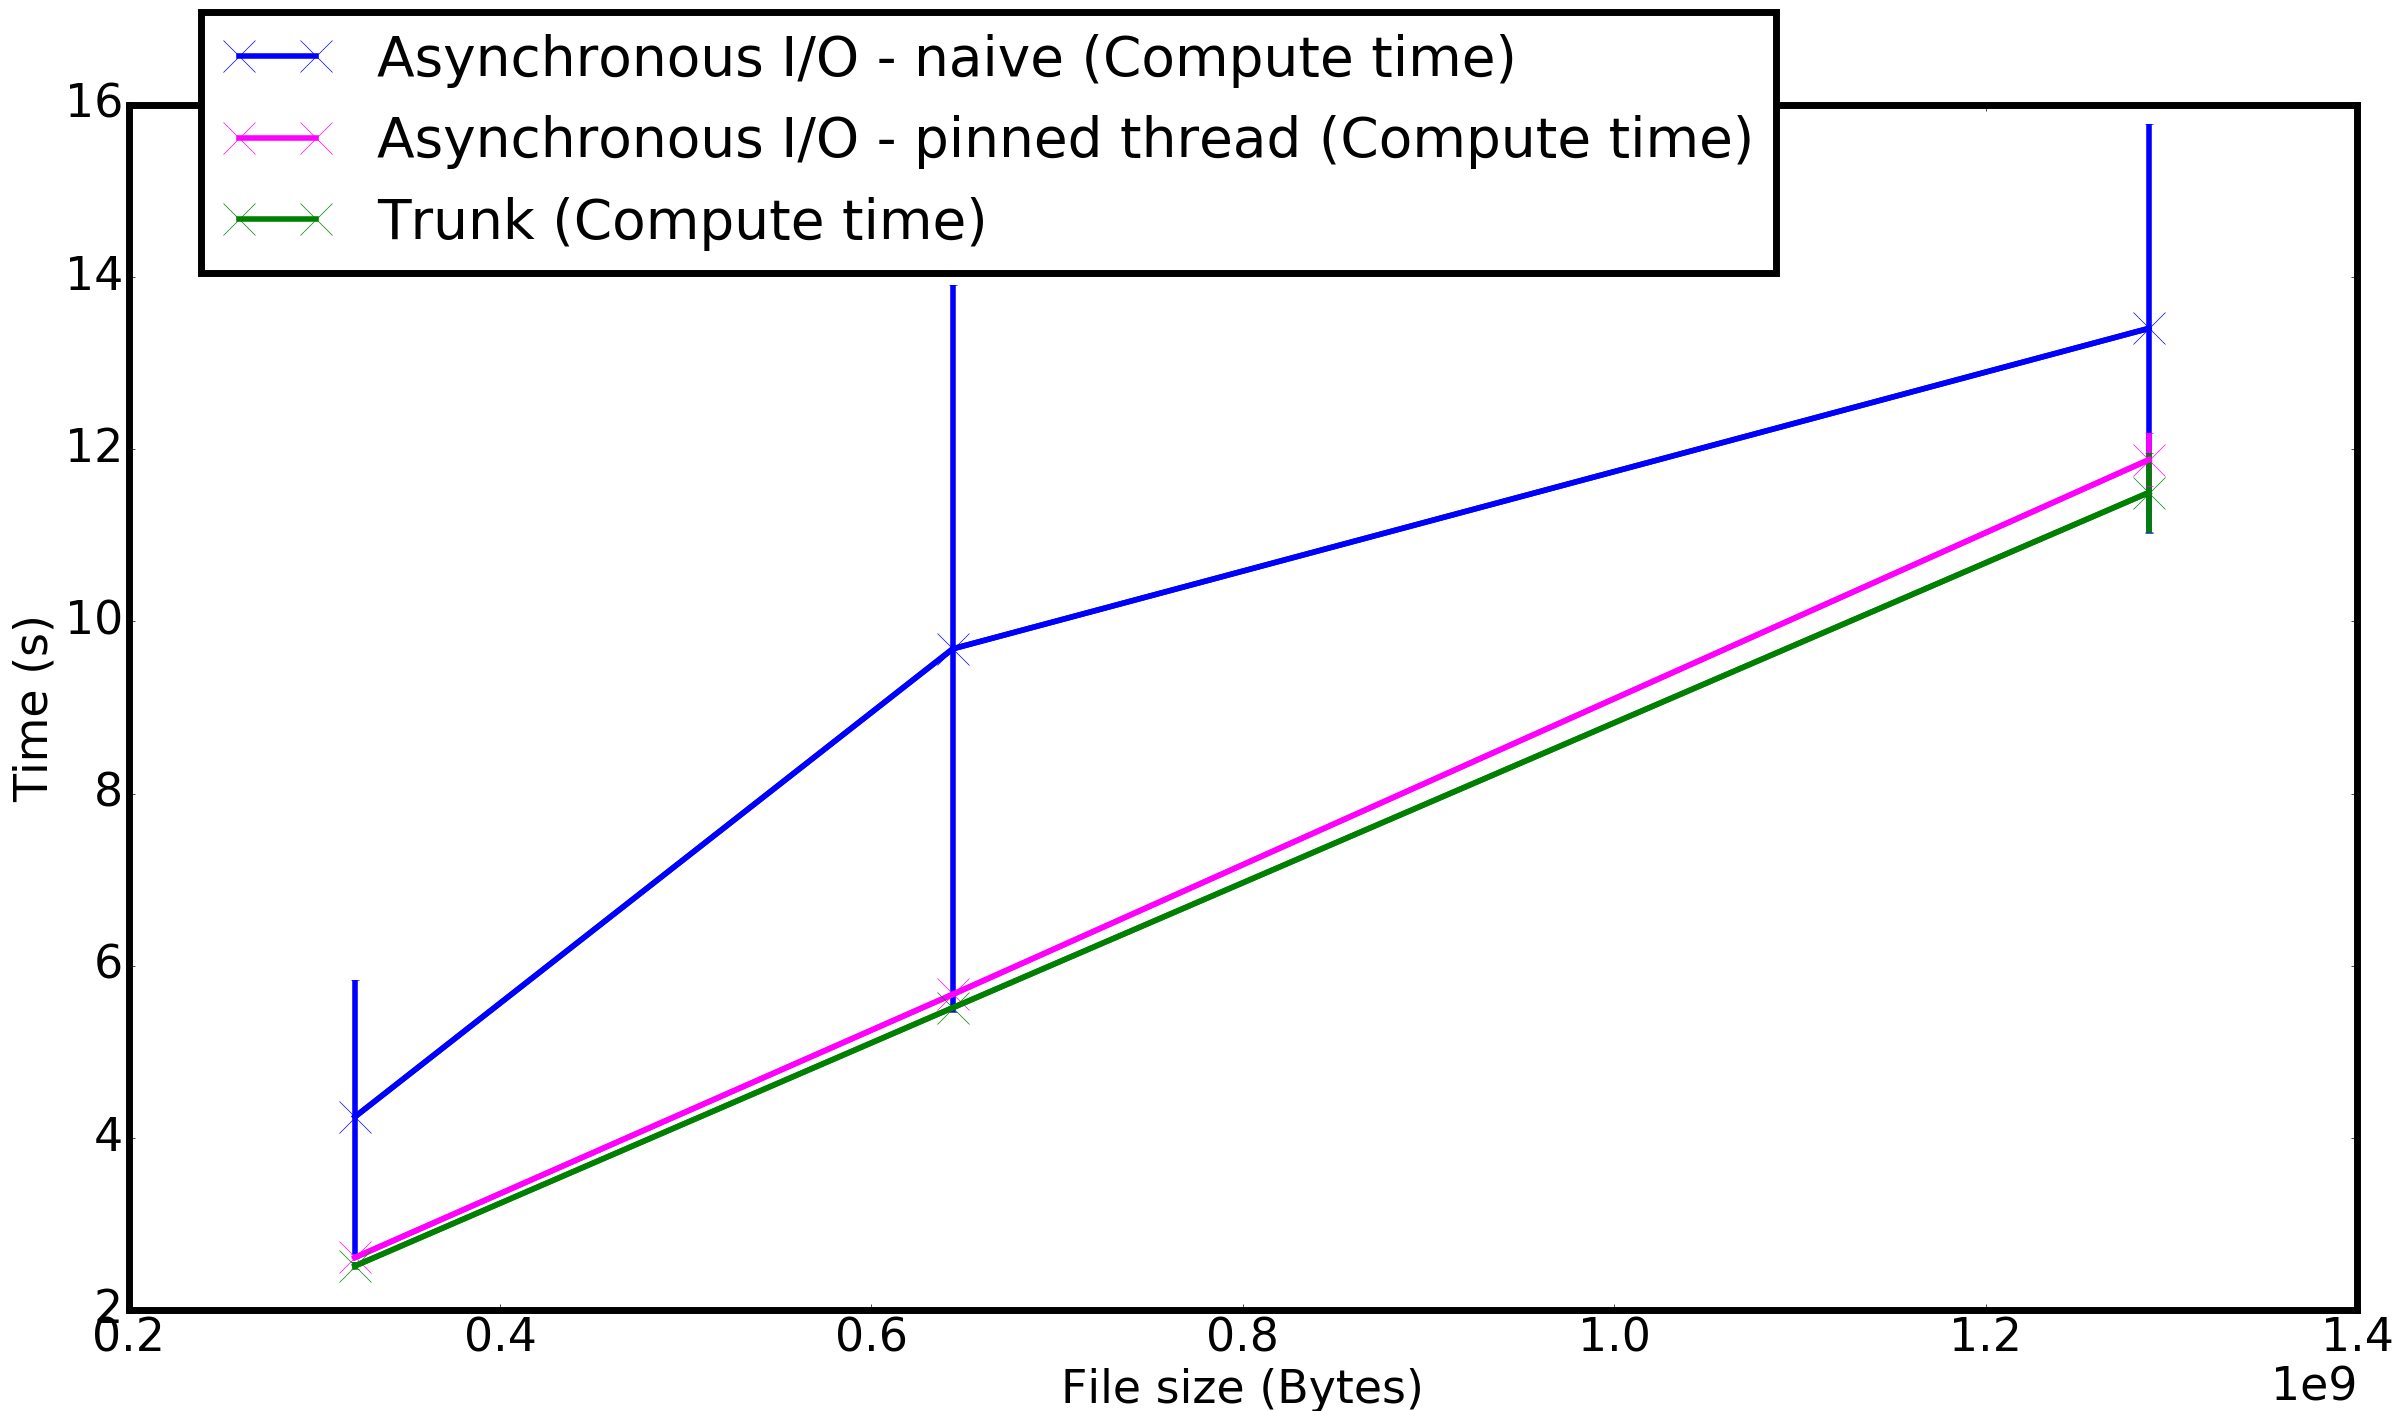
\includegraphics[width=\textwidth]{charts/cubeRemapper_pthreadWrap_compute_hpc.png}
					\caption[]%
					{{\small \targetPlatformHpc \space @ \targetPlatformHpcFrequency}}
					\label{fig:cubeRemapper_pthreadWrap_compute_hpc}
				\end{subfigure}
				\vskip\baselineskip
				\begin{subfigure}[b]{0.475\textwidth}
					\centering
					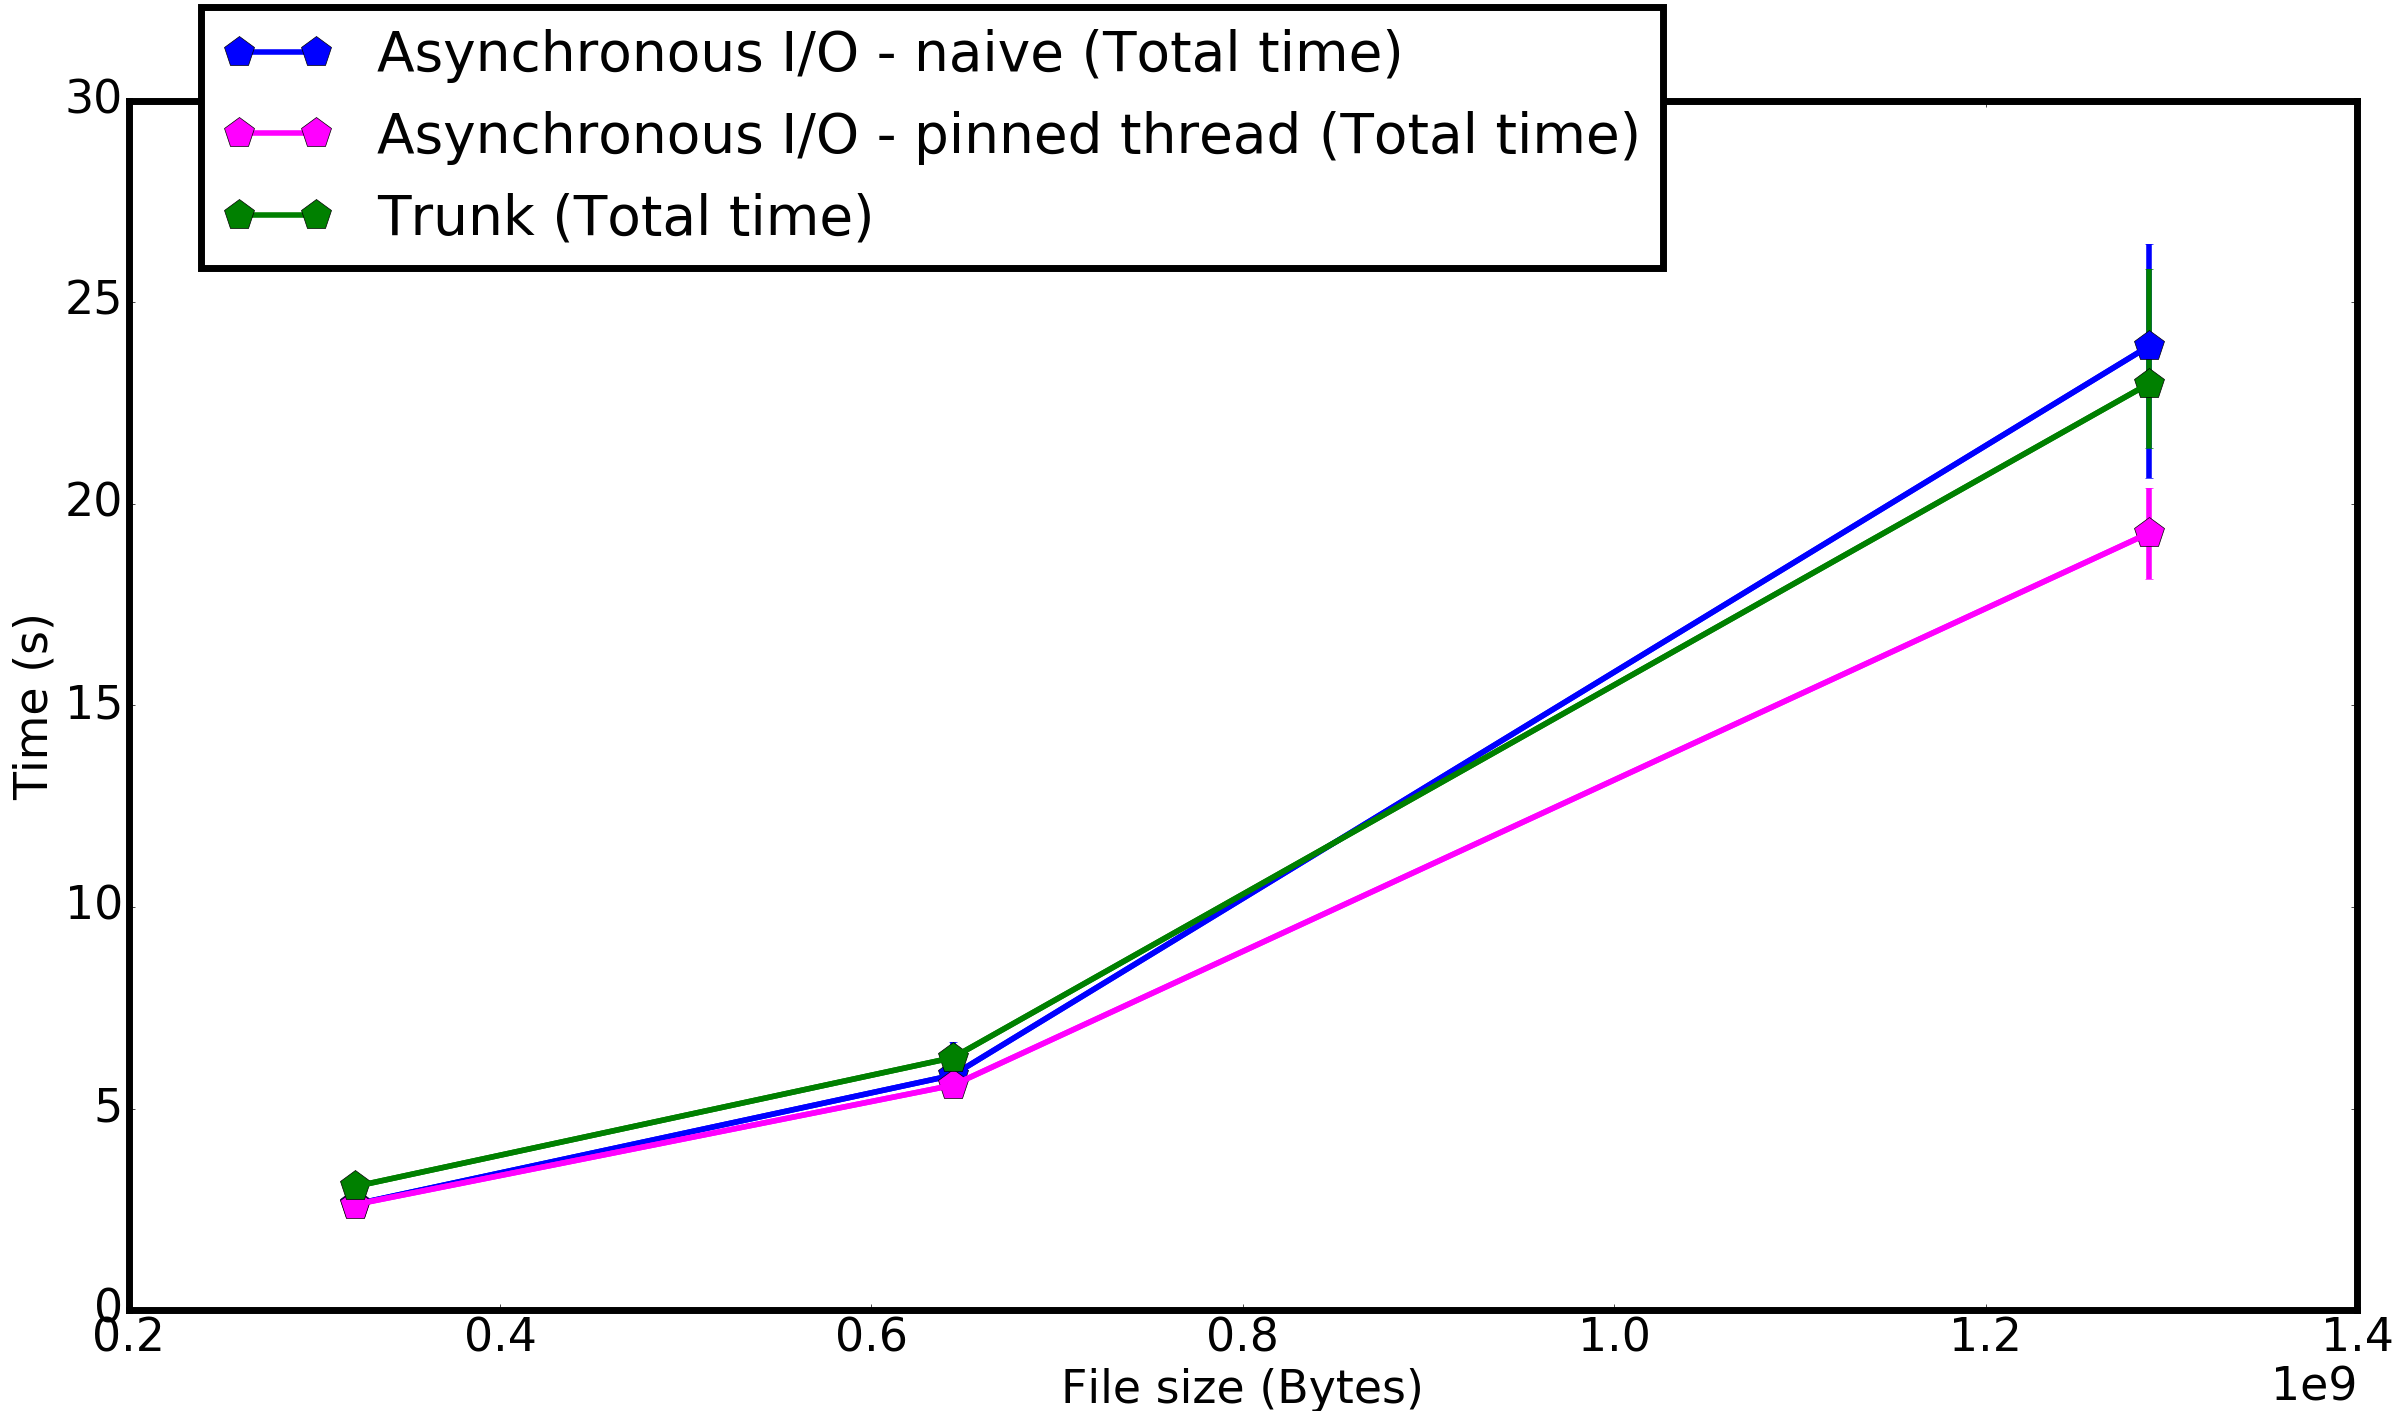
\includegraphics[width=\textwidth]{charts/cubeRemapper_pthreadWrap_total_workstation_8core.png}
					\caption[\targetPlatformLaptop \space @ \targetPlatformLaptopFrequency]
					{{\small \targetPlatformLaptop \space @ \targetPlatformLaptopFrequency}}
					\label{fig:cubeRemapper_pthreadWrap_total_workstation}
				\end{subfigure}
				\hfill
				\begin{subfigure}[b]{0.475\textwidth}
					\centering
					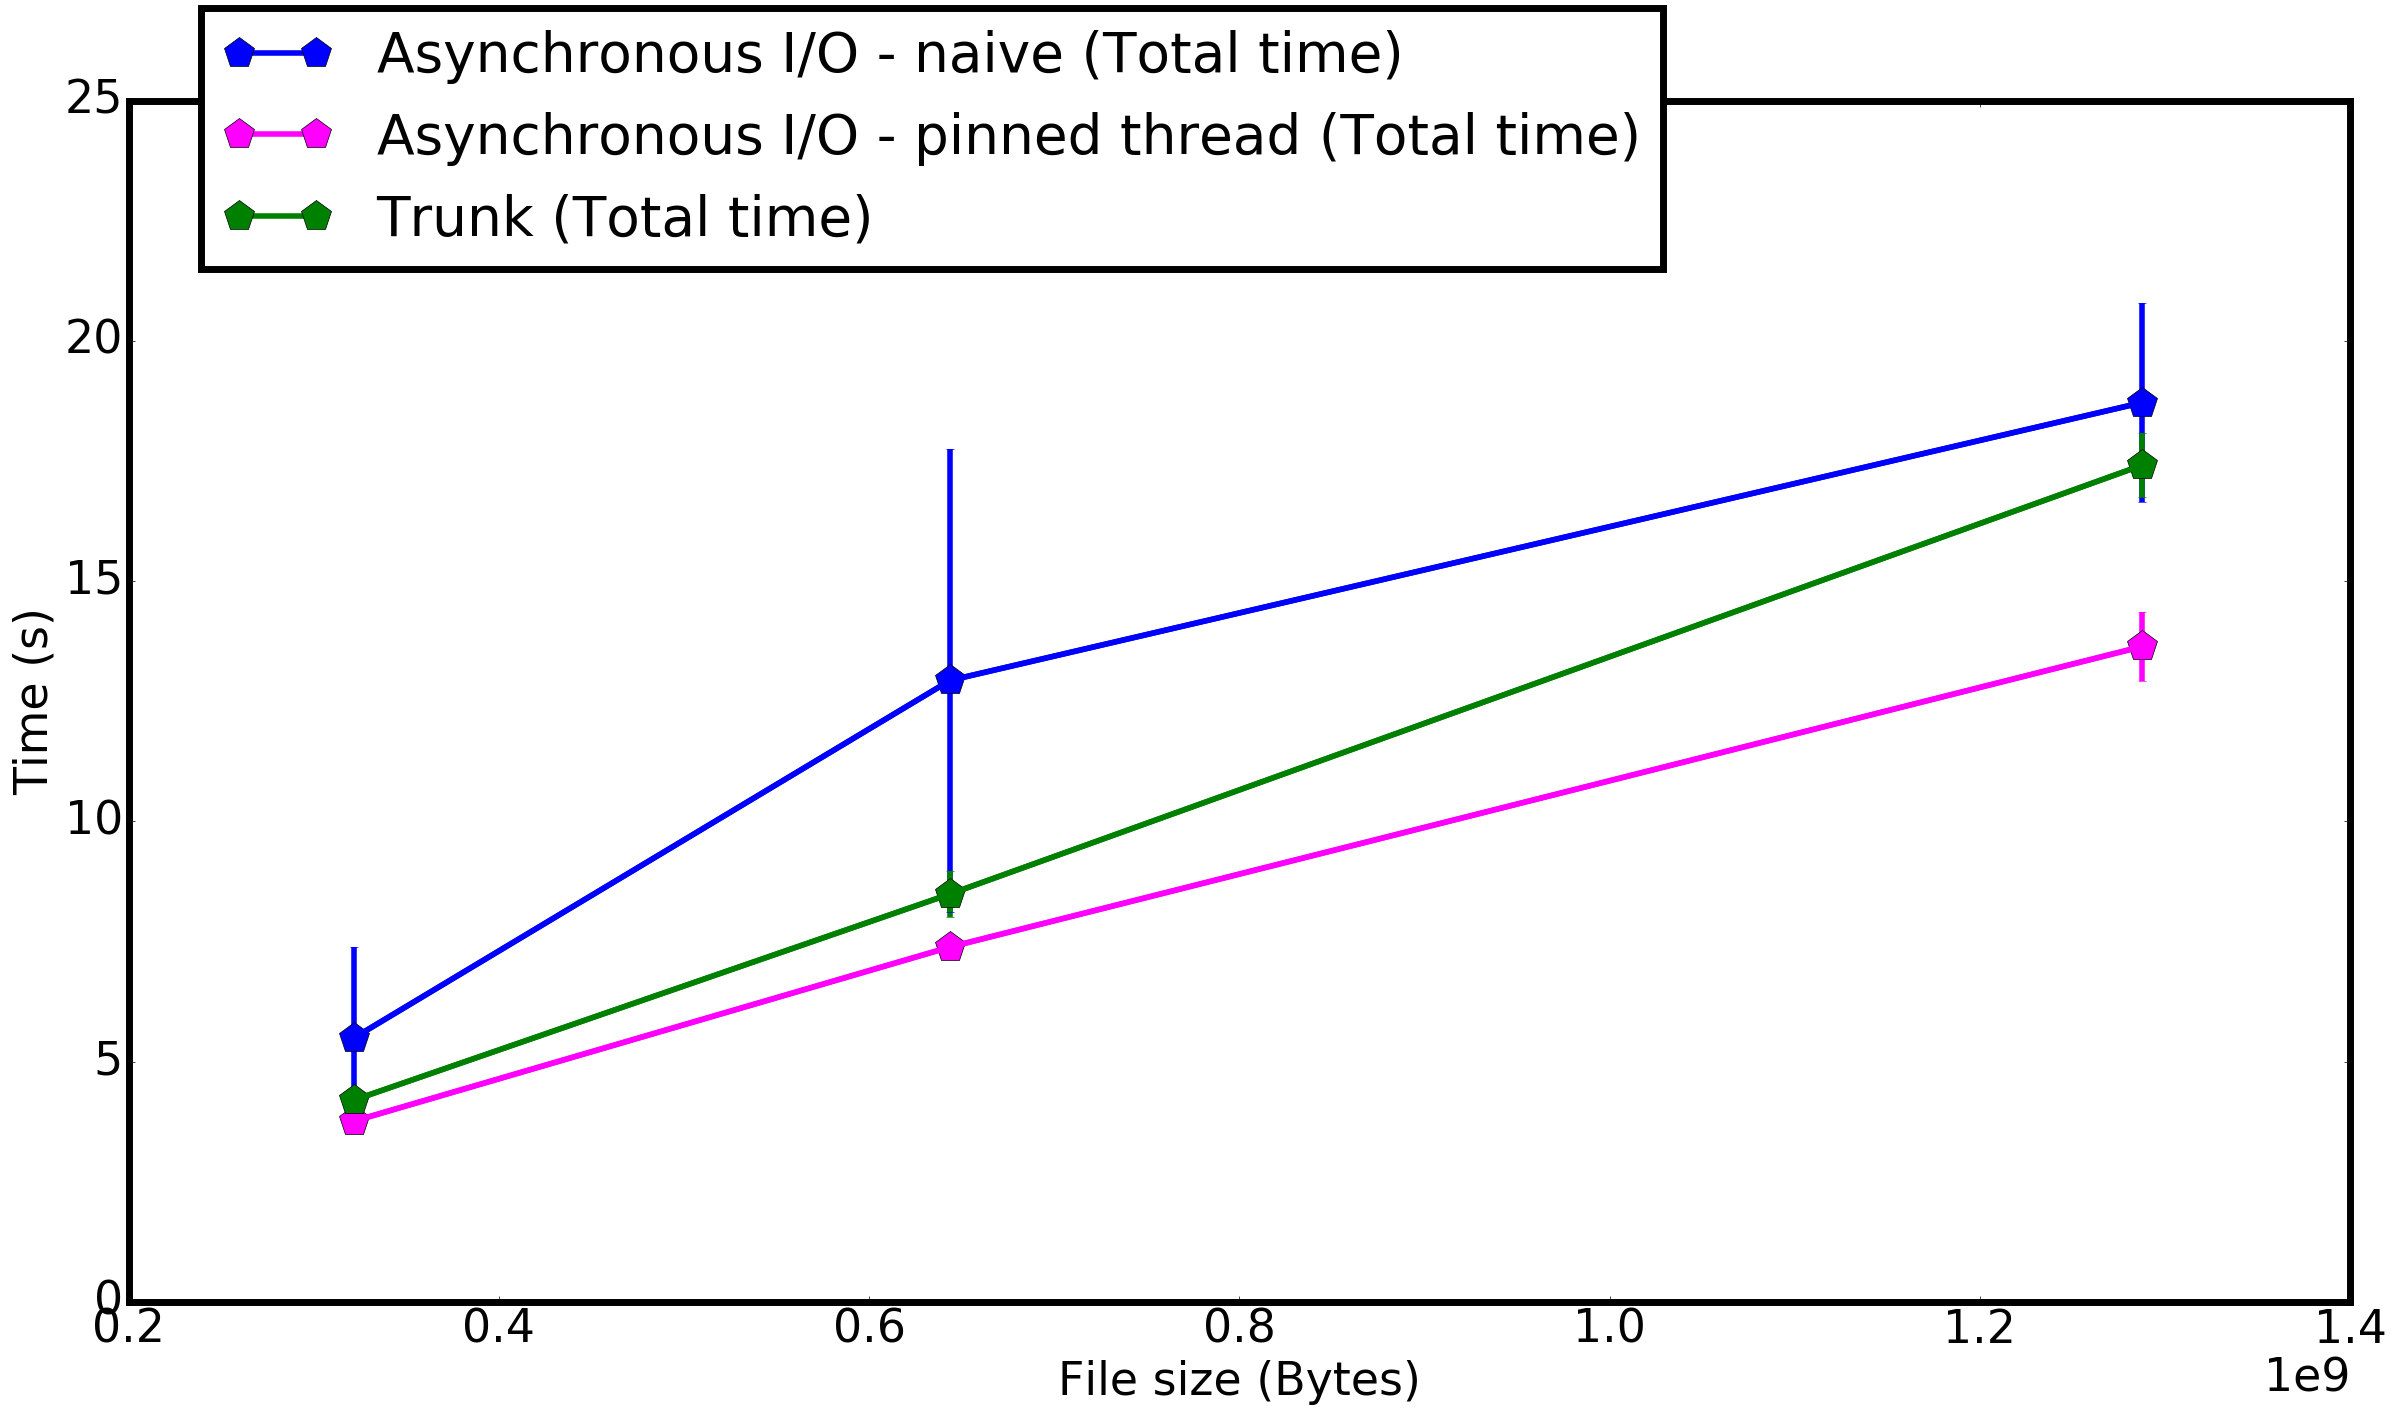
\includegraphics[width=\textwidth]{charts/cubeRemapper_pthreadWrap_total_hpc.png}
					\caption[]%
					{{\small \targetPlatformHpc \space @ \targetPlatformHpcFrequency}}
					\label{fig:cubeRemapper_pthreadWrap_total_hpc}
				\end{subfigure}
				\caption{Experimental comparison of the \emph{compute} and \emph{total} time: proposed \emph{\notationaio}\space (\emph{pinned thread}) VS. proposed \emph{\notationaio}\space (naive) VS. \emph{state-of-the-art} (trunk synchronous) implementation of the \toolTargetSoftware}
				\label{fig:cubeRemapper_pthreadWrap}
			\end{figure*}

		Figure \ref{fig:cubeRemapper_pthreadWrap} shows the impact of setting the thread affinity on the \emph{compute} operation in our custom implementation.   Indeed, Figures \ref{fig:cubeRemapper_pthreadWrap_compute_workstation} and \ref{fig:cubeRemapper_pthreadWrap_compute_hpc} show that the gap between the response time of the \emph{compute} operation in our enhanced custom implementation and the state-of-the-art one has been decreased to respectively $5$ and $2\%$ (compared to that of Figures \ref{fig:cubeRemapper_basicImplementation_compute_workstation_8core} and \ref{fig:cubeRemapper_basicImplementation_compute_hpc}) on the \targetPlatformHpc and the \targetPlatformLaptop platforms.\\
		Likewise, the size of the fluctuation of this operation has significantly collapsed (compared to that of Figure \ref{fig:cubeRemapper_basicImplementation_compute_workstation_8core} and \ref{fig:cubeRemapper_basicImplementation_compute_hpc}).\\
		Consequently, the overall gain achieved by our enhanced asynchronous strategy is now clearly confirmed.   In Figures \ref{fig:cubeRemapper_pthreadWrap_total_workstation} and \ref{fig:cubeRemapper_pthreadWrap_total_hpc}, the total time of our implementation is about $60\%$  more efficient than that of the state-of-the-art.   Moreover, the error margin of the \emph{compute} operation has been dramatically reduced.   Thus, the observed overall improvement is now clearly achieved and in a more robust manner (regardless of the error margin).


	\subsection{Reducing the impact of false-sharing} \label{subsection:lightenFalseSharing}
		Despite our effort to reduce the number of shared memory addresses and reduce the impact of synchronization between threads, Figures \ref{fig:cubeRemapper_basicImplementation_compute_total} and \ref{fig:cubeRemapper_pthreadWrap} show that the overhead due to synchronization might still be reduced\footnote{The execution time of the \emph{compute} function in our implementation is still slightly higher than the one in the \emph{state-of-the-art} implementation}.   Given that we managed to use independent buffers between concurrent threads (RAM level), our explanation is that this interference is due to \emph{false-sharing} (cache level).\\

		In Figures \ref{fig:cubeRemapper_falseSharing_compute_L3_workstation_8core} and \ref{fig:cubeRemapper_falseSharing_compute_L3_hpc}, we have represented the cache access foot-print of each one of the \emph{state-of-the-art} (\emph{trunk}), the \emph{naive} and the \emph{aligned buffer} implementations of the \toolTargetSoftware.   As one can notice, the number of cache misses in the \emph{naive} version of the code is about $33\%$ higher than that of the \emph{state-of-the-art} one.   Given that these two curves profile the same implementation of the \emph{compute} function, this shows the impact of \emph{false-sharing} on our implementation.   This result is also correlated with the one at time level (Figure \ref{fig:cubeRemapper_falseSharing_compute_time_workstation_8core} and \ref{fig:cubeRemapper_falseSharing_compute_time_hpc}).\\

			\begin{figure*}[!h]
				\centering
				\begin{subfigure}[b]{0.475\textwidth}
					\centering
					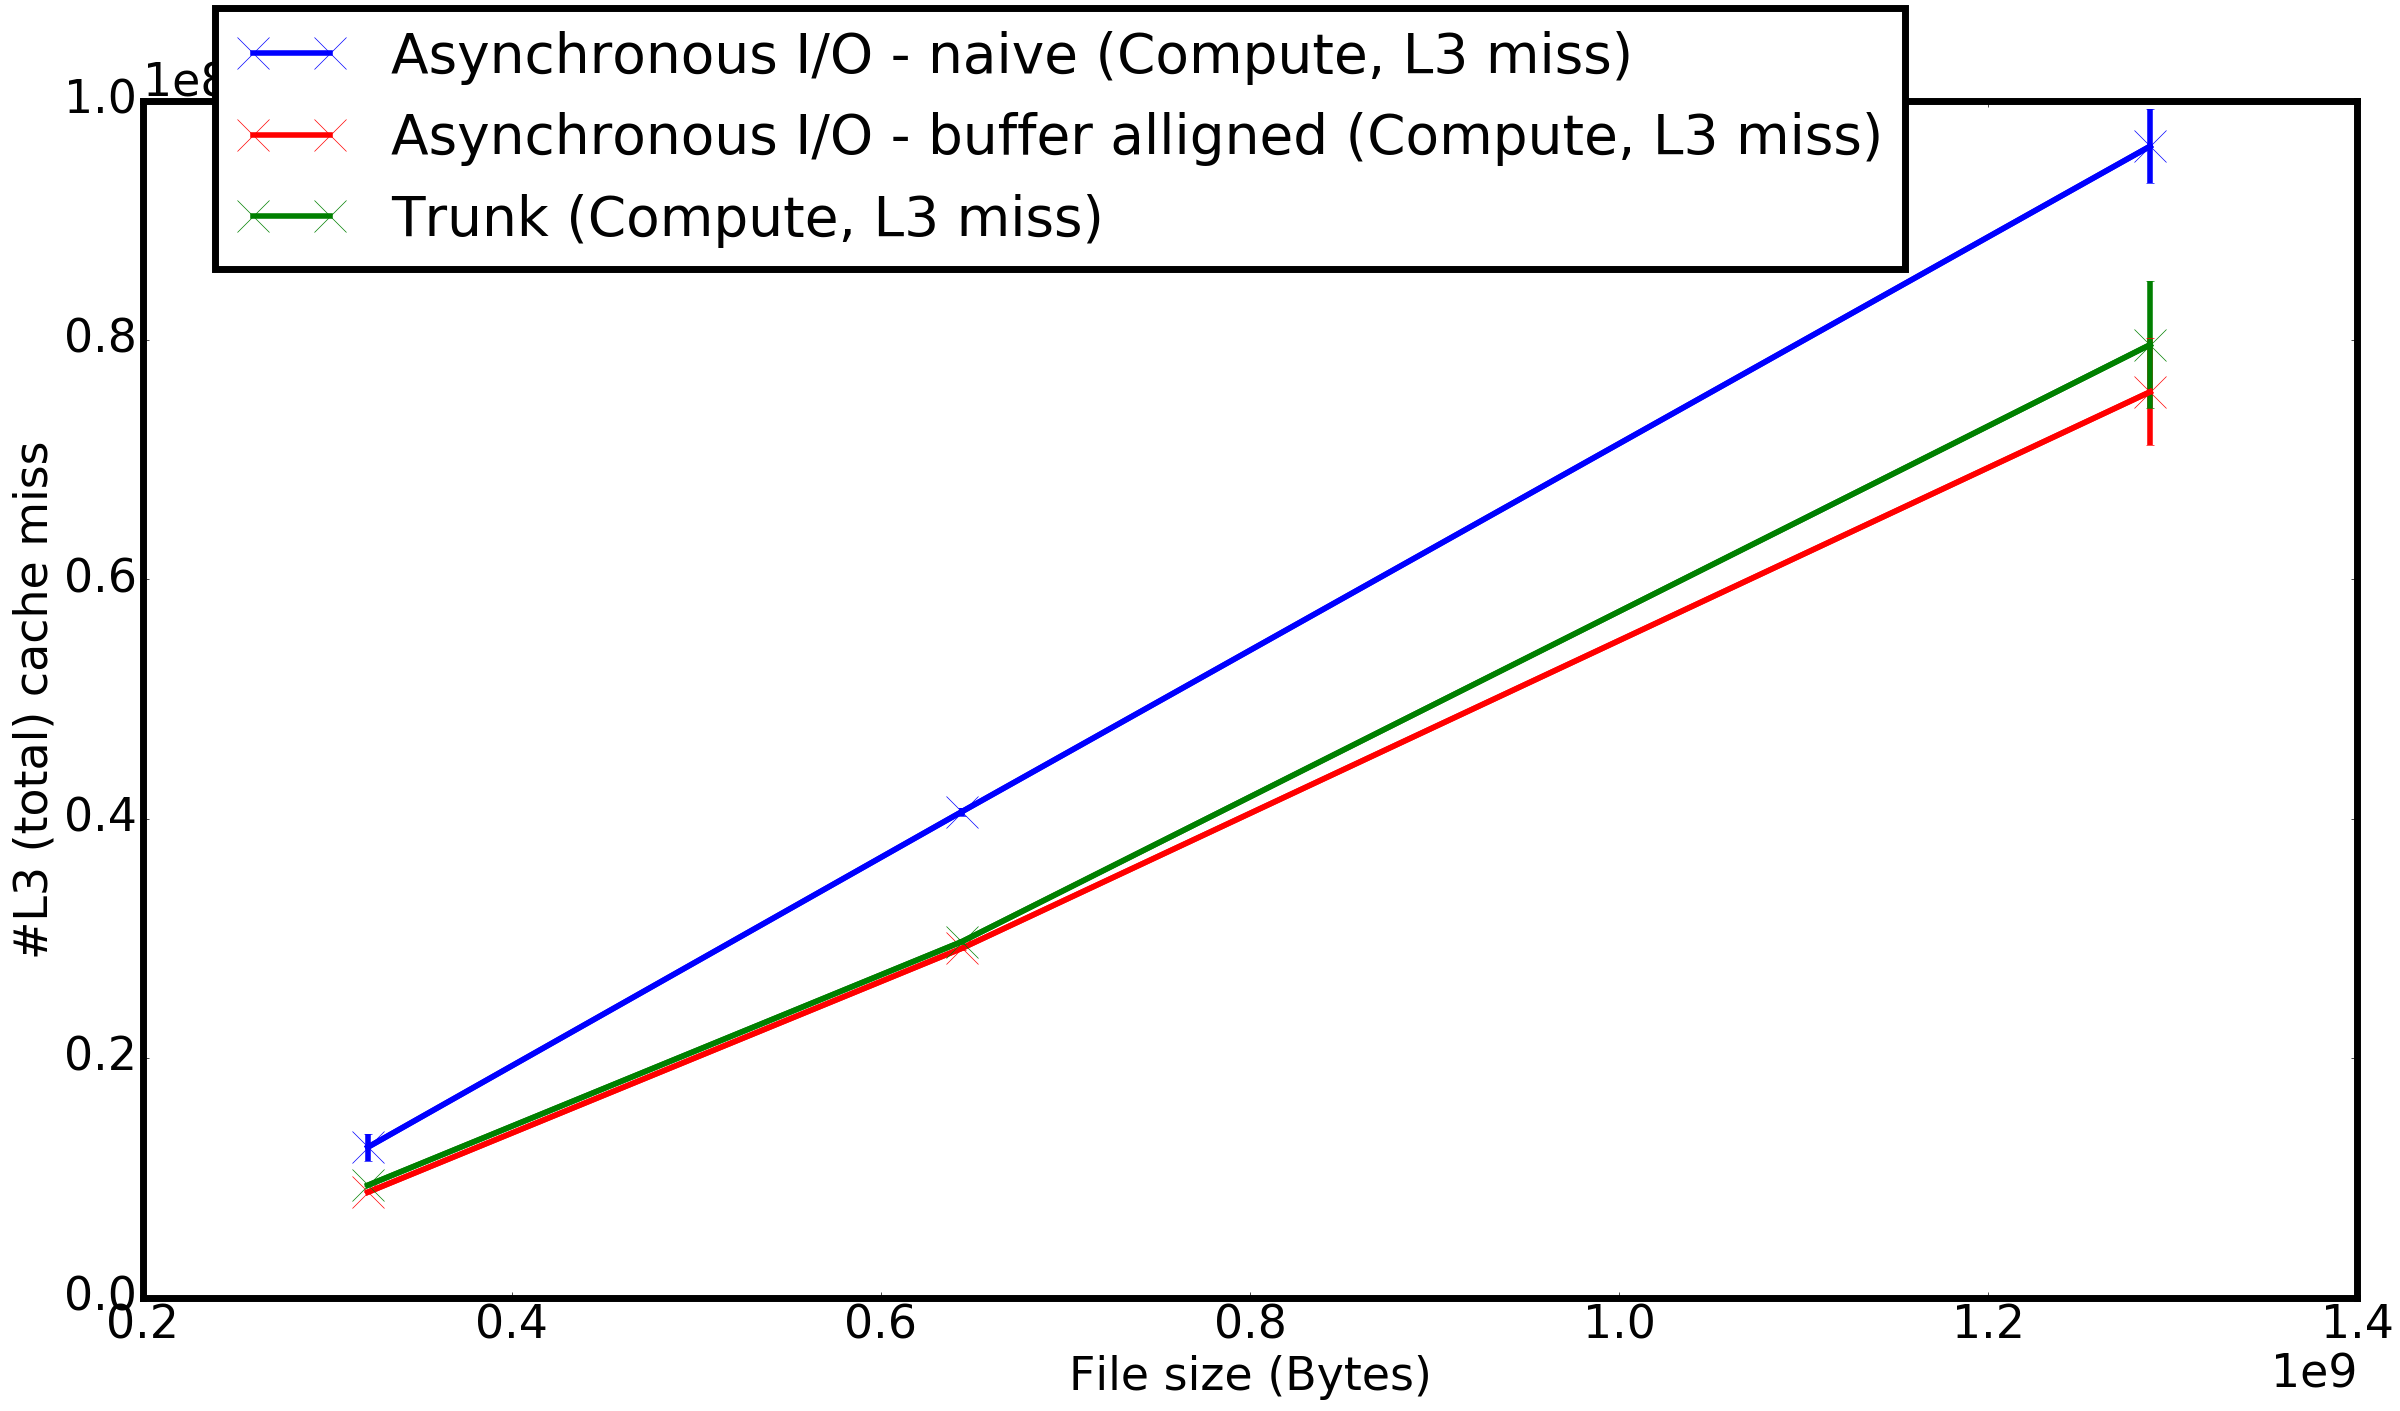
\includegraphics[width=\textwidth]{charts/cubeRemapper_falseSharing_compute_trackL3_workstation_8core.png}
					\caption[\targetPlatformLaptop \space @ \targetPlatformLaptopFrequency]
					{{\small \targetPlatformLaptop \space @ \targetPlatformLaptopFrequency}}
					\label{fig:cubeRemapper_falseSharing_compute_L3_workstation_8core}
				\end{subfigure}
				\hfill
				\begin{subfigure}[b]{0.475\textwidth}  
					\centering
					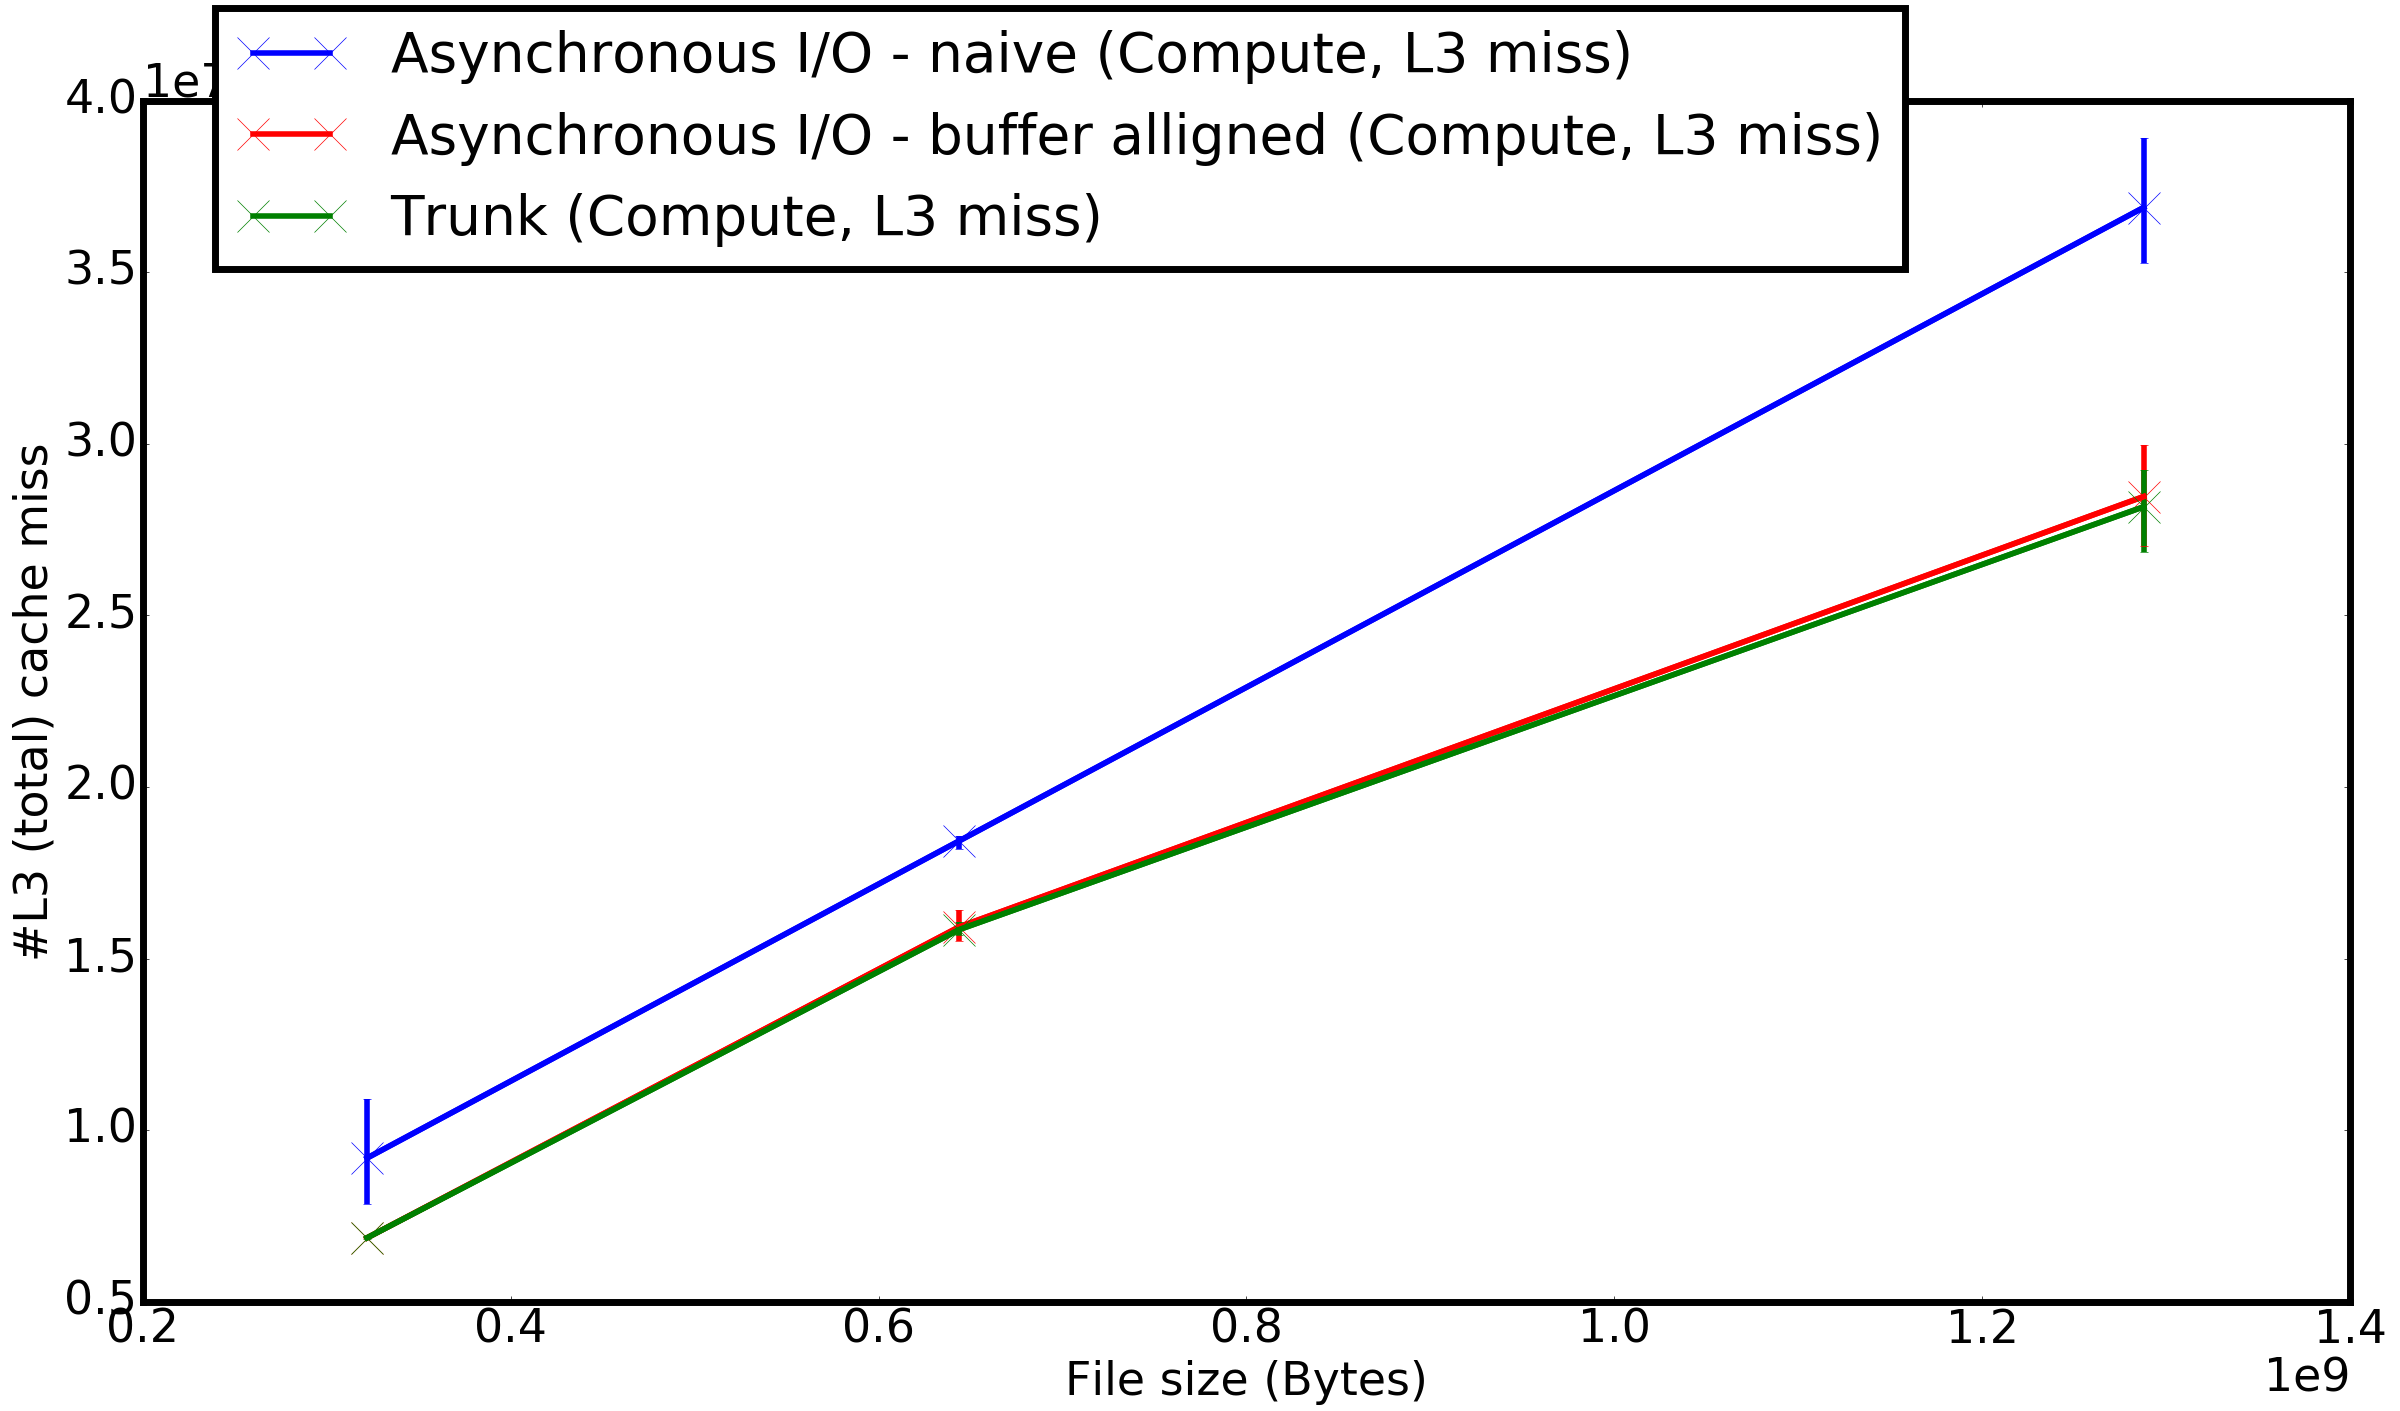
\includegraphics[width=\textwidth]{charts/cubeRemapper_falseSharing_compute_trackL3_hpc.png}
					\caption[]%
					{{\small \targetPlatformHpc \space @ \targetPlatformHpcFrequency}}
					\label{fig:cubeRemapper_falseSharing_compute_L3_hpc}
				\end{subfigure}
				\vskip\baselineskip
				\begin{subfigure}[b]{0.475\textwidth}
					\centering
					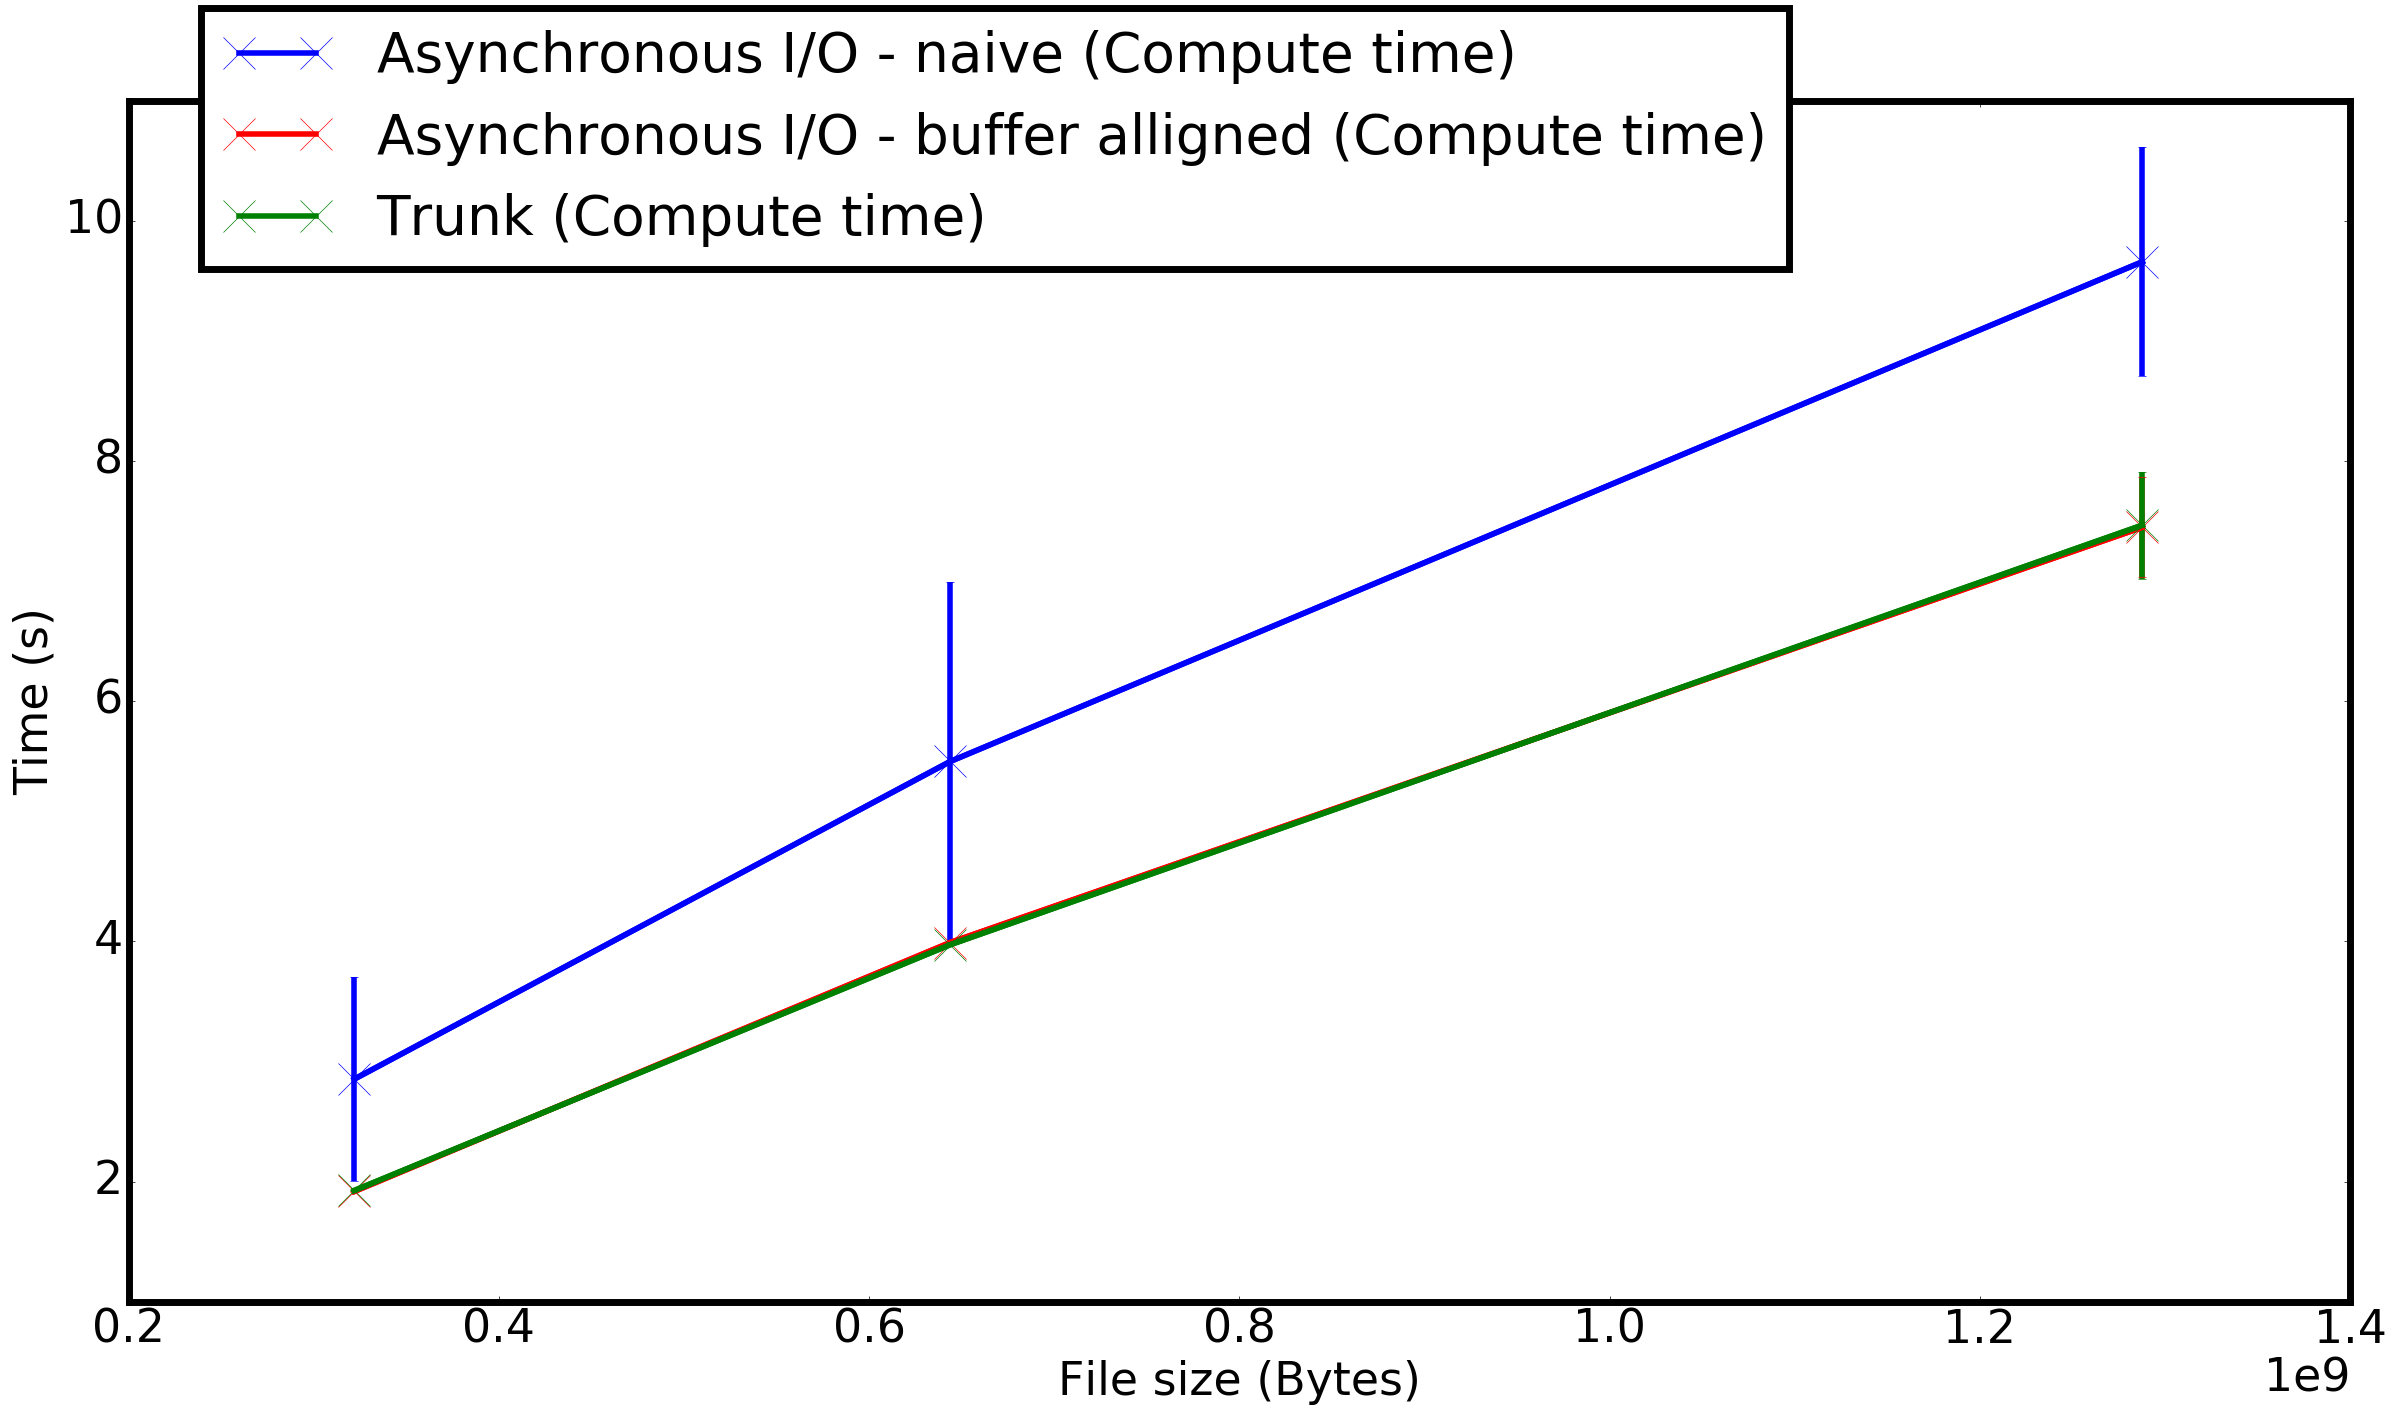
\includegraphics[width=\textwidth]{charts/cubeRemapper_falseSharing_compute_time_workstation_8core.png}
					\caption[]%
					{{\small \targetPlatformLaptop @ \targetPlatformLaptopFrequency}}
					\label{fig:cubeRemapper_falseSharing_compute_time_workstation_8core}
				\end{subfigure}
				\hfill
				\begin{subfigure}[b]{0.475\textwidth}  
					\centering 
					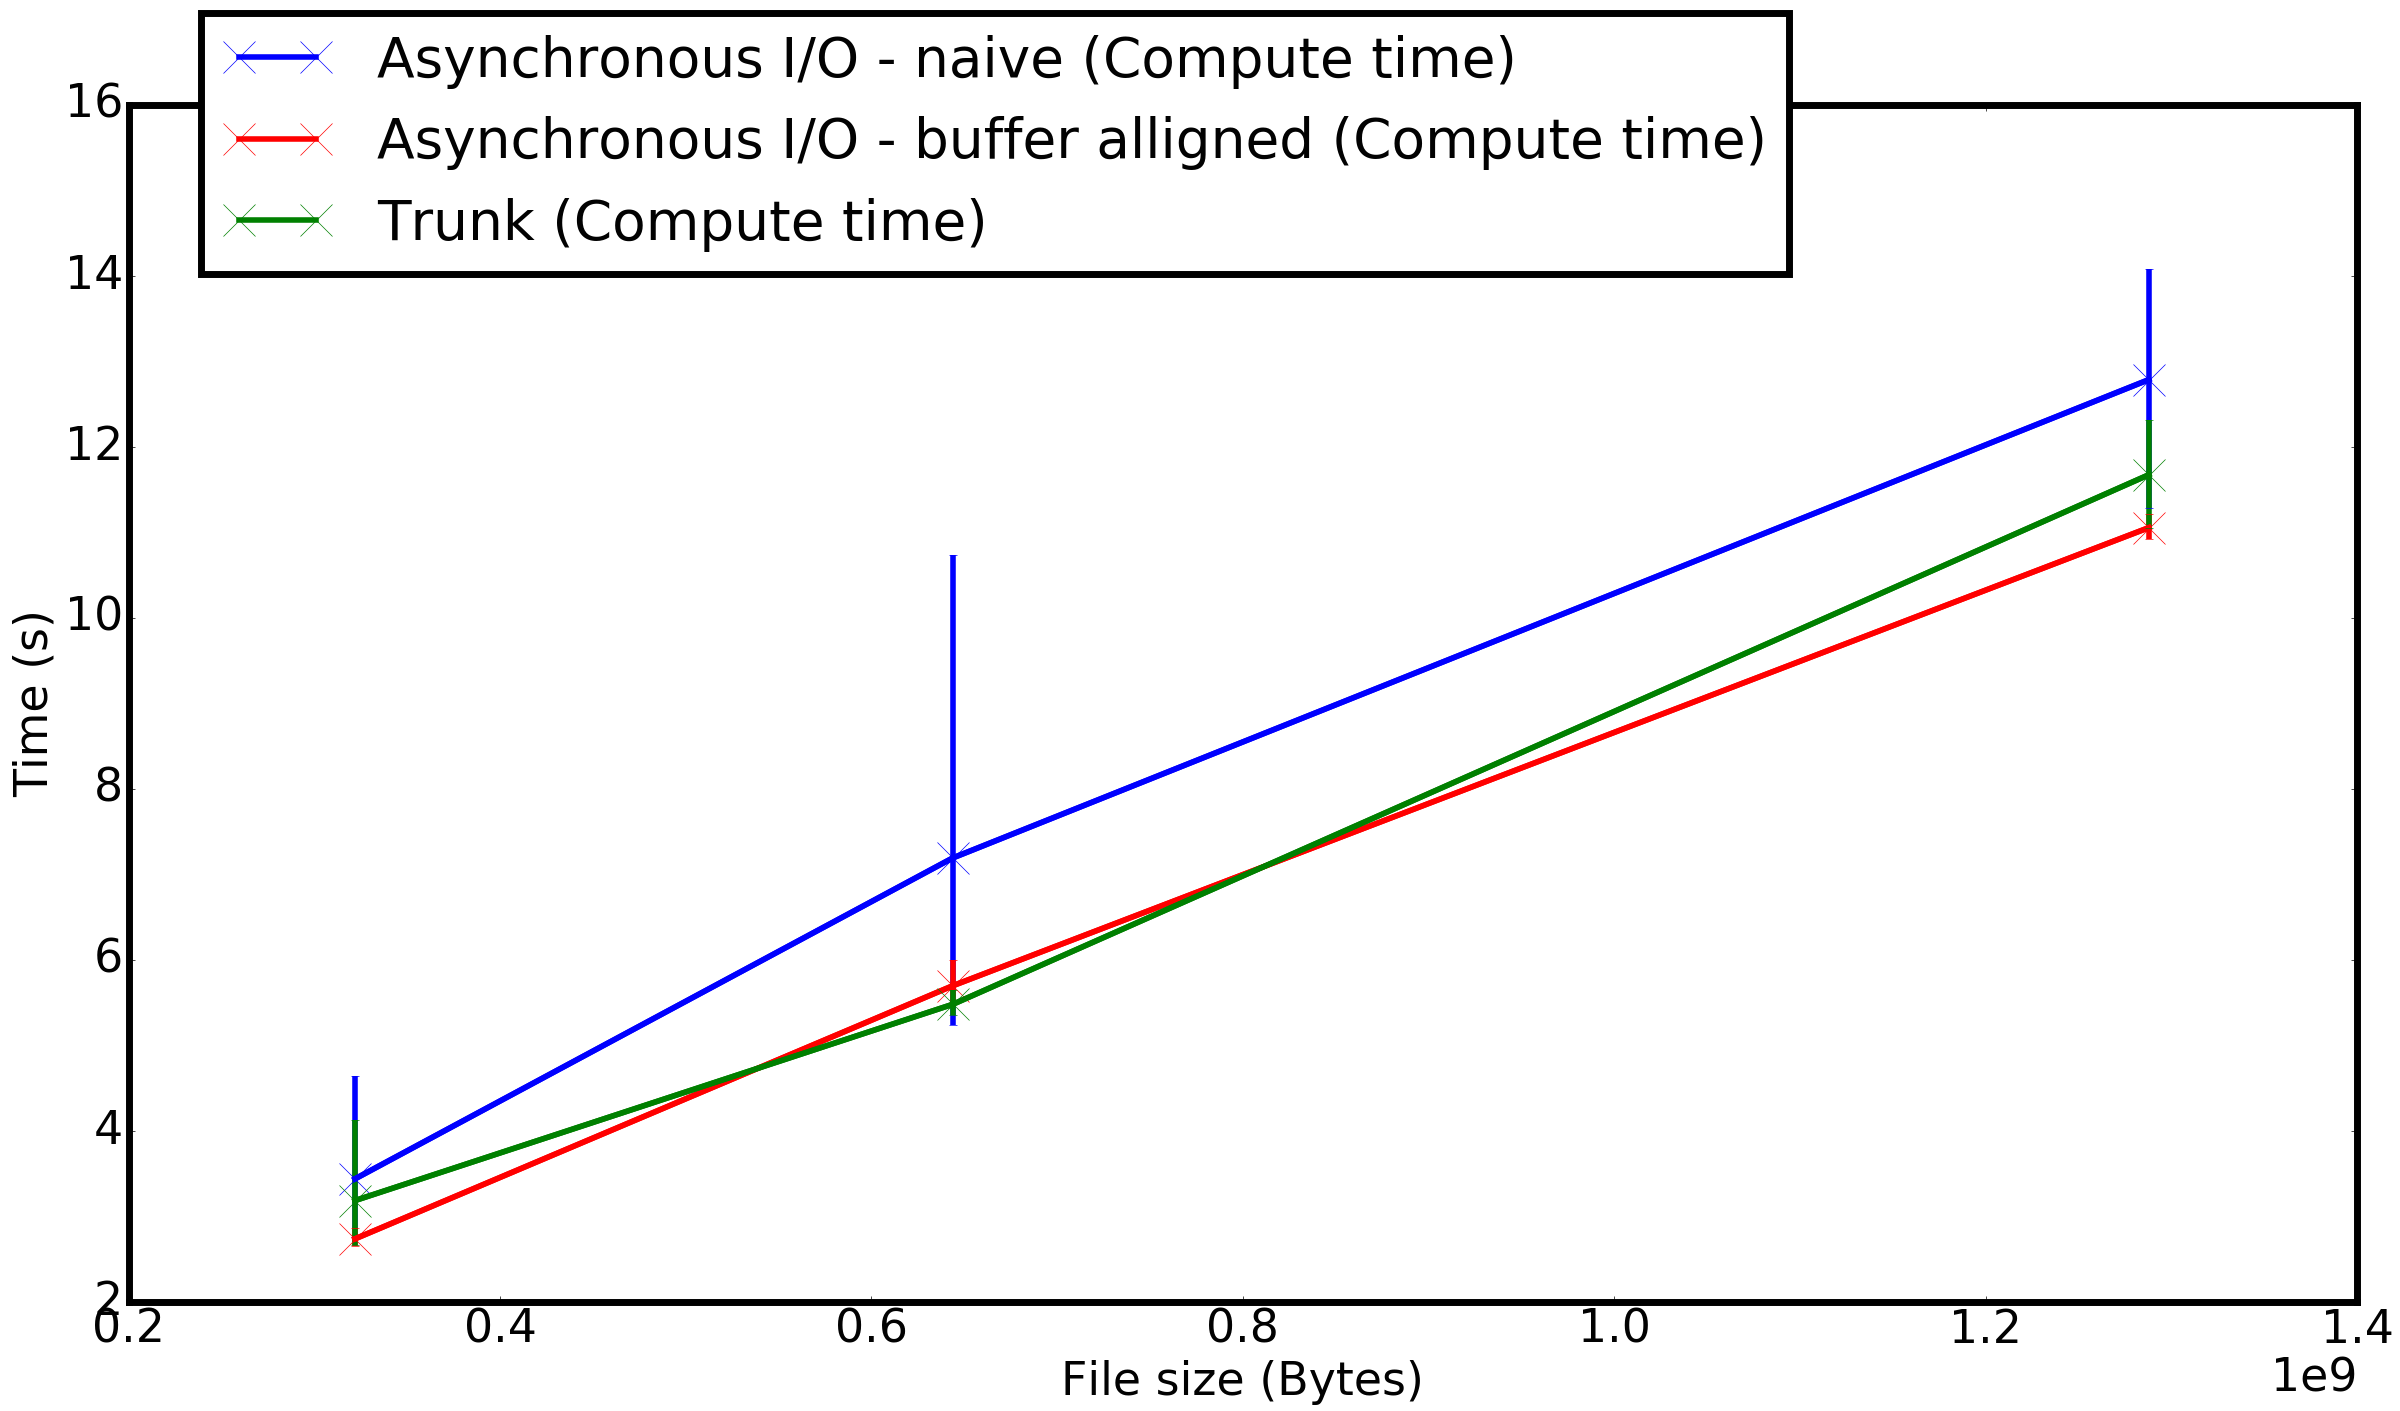
\includegraphics[width=\textwidth]{charts/cubeRemapper_falseSharing_compute_time_hpc.png}
					\caption[]%
					{{\small \targetPlatformHpc \space @ \targetPlatformHpcFrequency}}
					\label{fig:cubeRemapper_falseSharing_compute_time_hpc}
				\end{subfigure}
				\caption{Experimental comparison of the \emph{L3 cache-miss} (total) and \emph{compute} time: proposed \emph{\notationaio}\space (buffer aligned) VS. proposed \emph{\notationaio}\space (naive) VS. \emph{state-of-the-art} (trunk synchronous) implementation of the \toolTargetSoftware.   For the seek of clarity the only results represented are the one linked to the \emph{compute} operation}
				\label{fig:cubeRemapper_falseSharing_compute}
			\end{figure*}

		Furthermore, we see in Figures \ref{fig:cubeRemapper_falseSharing_compute_L3_workstation_8core} and \ref{fig:cubeRemapper_falseSharing_compute_L3_hpc} that the rate of cache misses in our \emph{buffer aligned} version drops down to the same level as that of the \emph{state-of-the-art} implementation.    Thus, our improvement allows to eliminate the cache-linked interferences between concurrent threads.\\
		This improvement, noticed at cache level, has a clear impact on the overall performance of our implementation.   Indeed, we observe in Figure \ref{fig:cubeRemapper_falseSharing_overall_time} an average gain of $70\%$ of the total time.   Given the increase of the stability in the performance of this \emph{buffer aligned} implementation, this gain is achieved regardless of the error margin.

			\begin{figure*}[!h]
				\centering
				\begin{subfigure}[b]{0.475\textwidth}
					\centering
					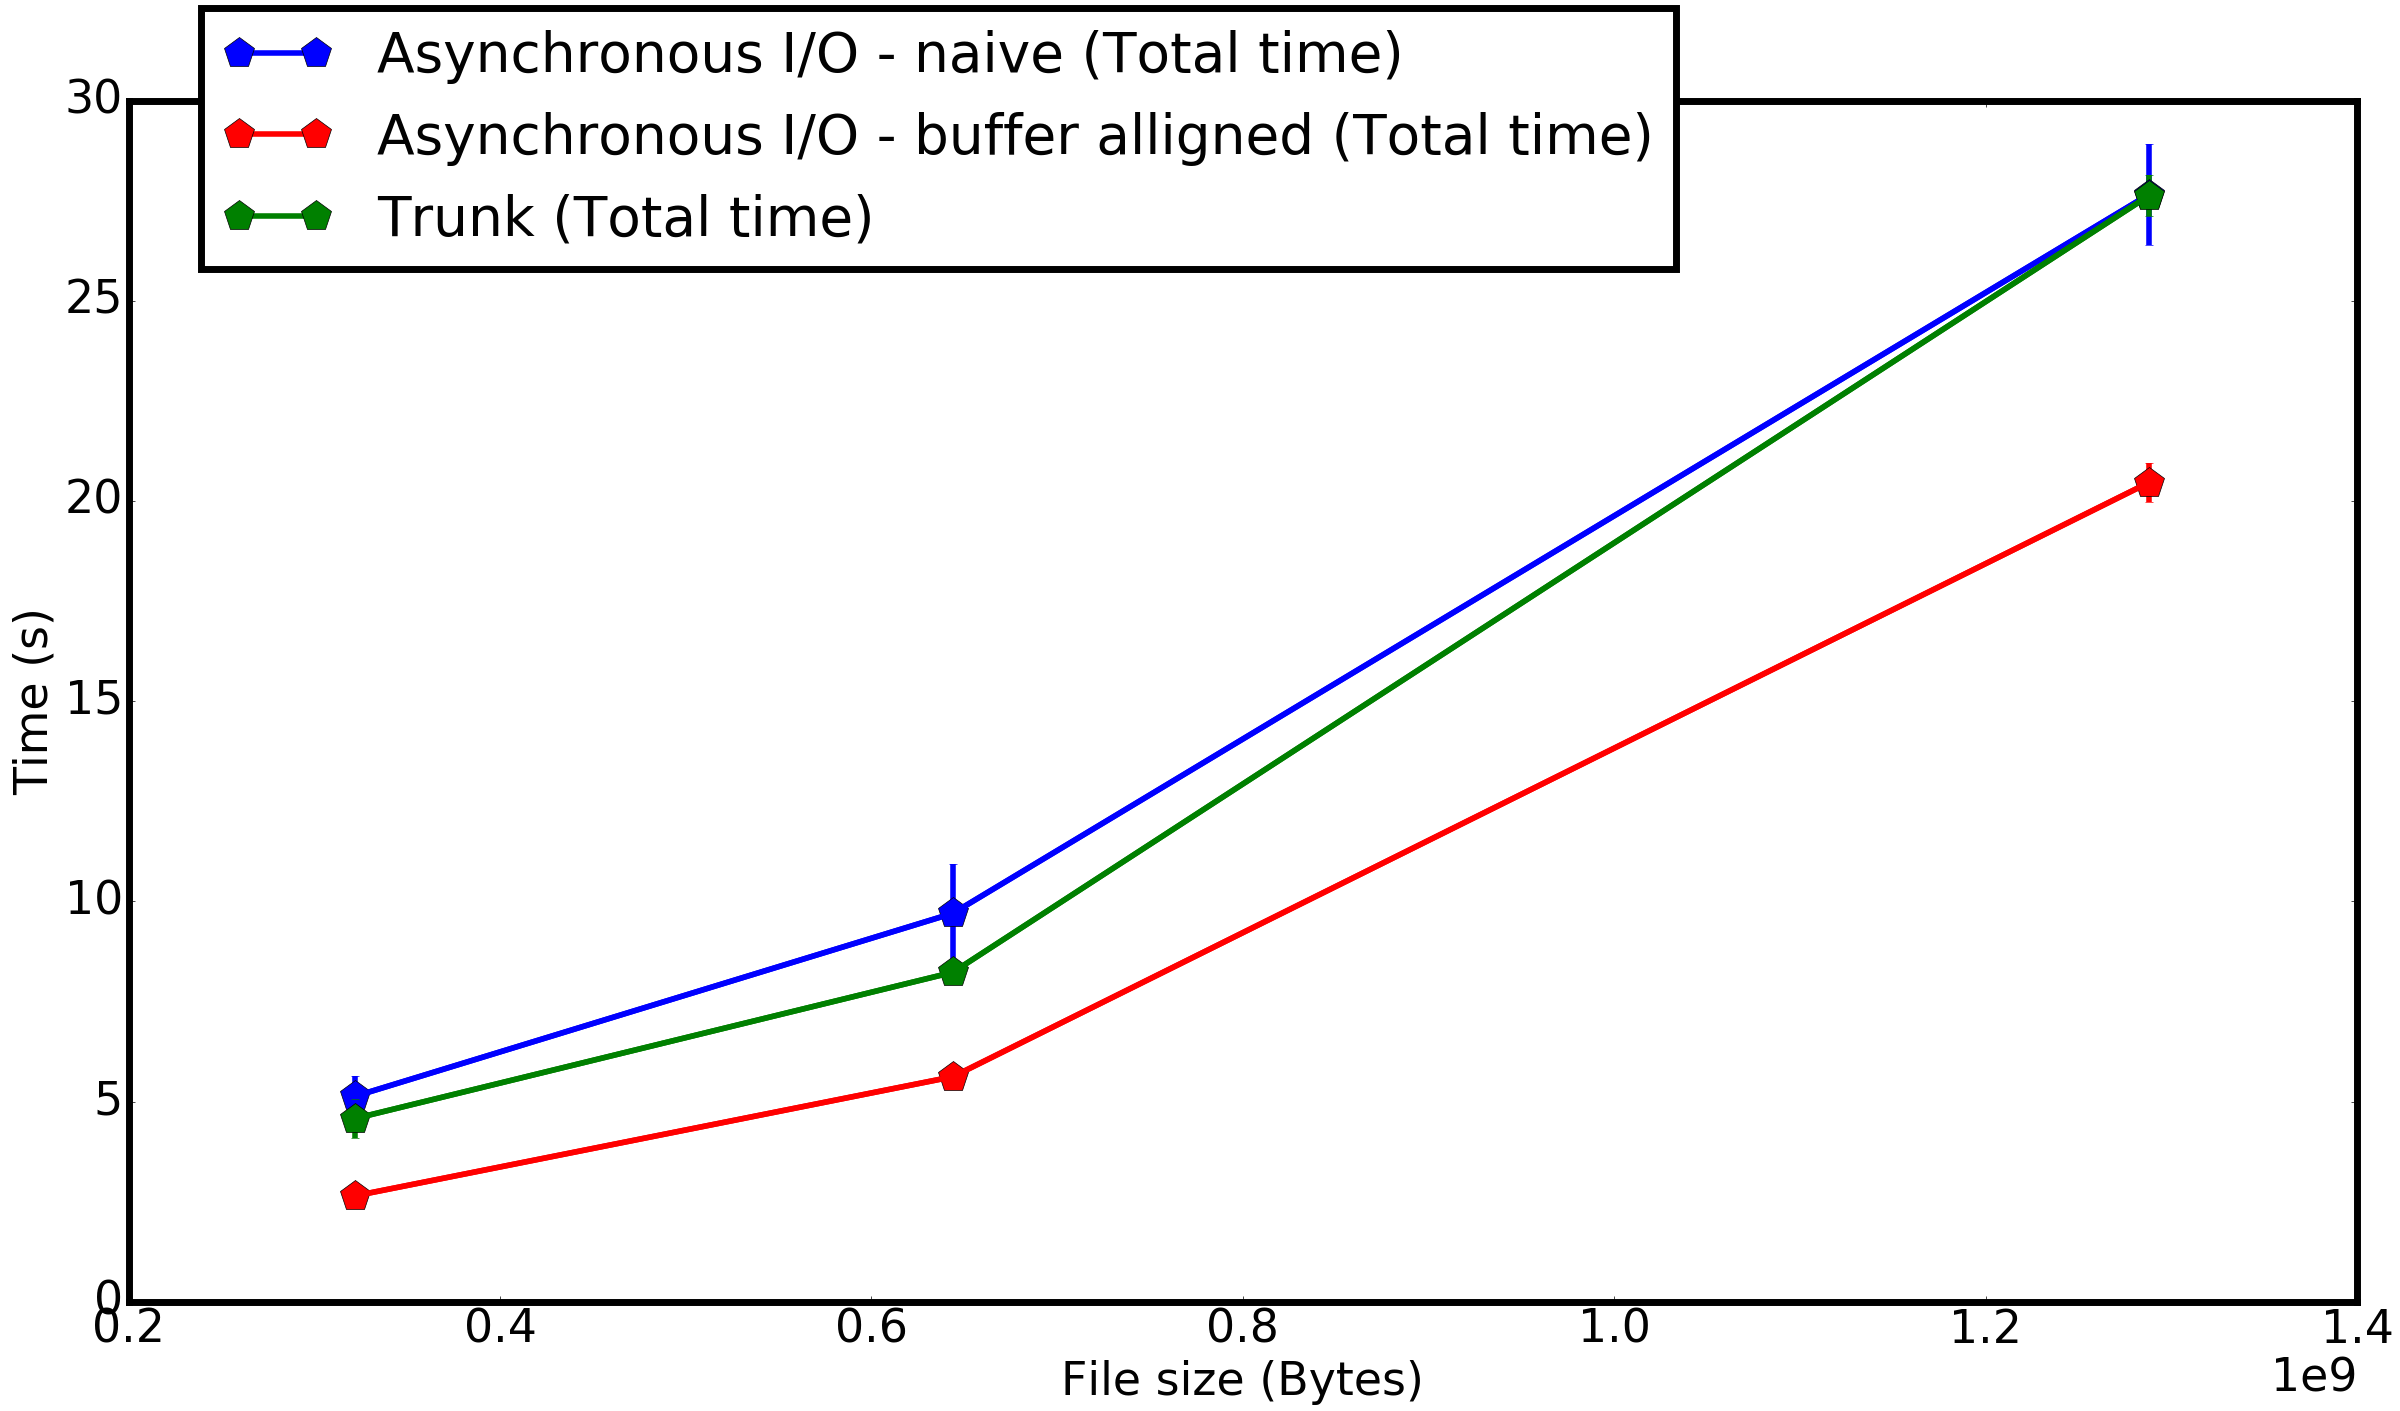
\includegraphics[width=\textwidth]{charts/cubeRemapper_falseSharing_overall_time_workstation_8core.png}
					\caption[\targetPlatformLaptop \space @ \targetPlatformLaptopFrequency]
					{{\small \targetPlatformLaptop \space @ \targetPlatformLaptopFrequency}}
					\label{fig:cubeRemapper_falseSharing_overall_time_workstation_8core}
				\end{subfigure}
				\hfill
				\begin{subfigure}[b]{0.475\textwidth}  
					\centering
					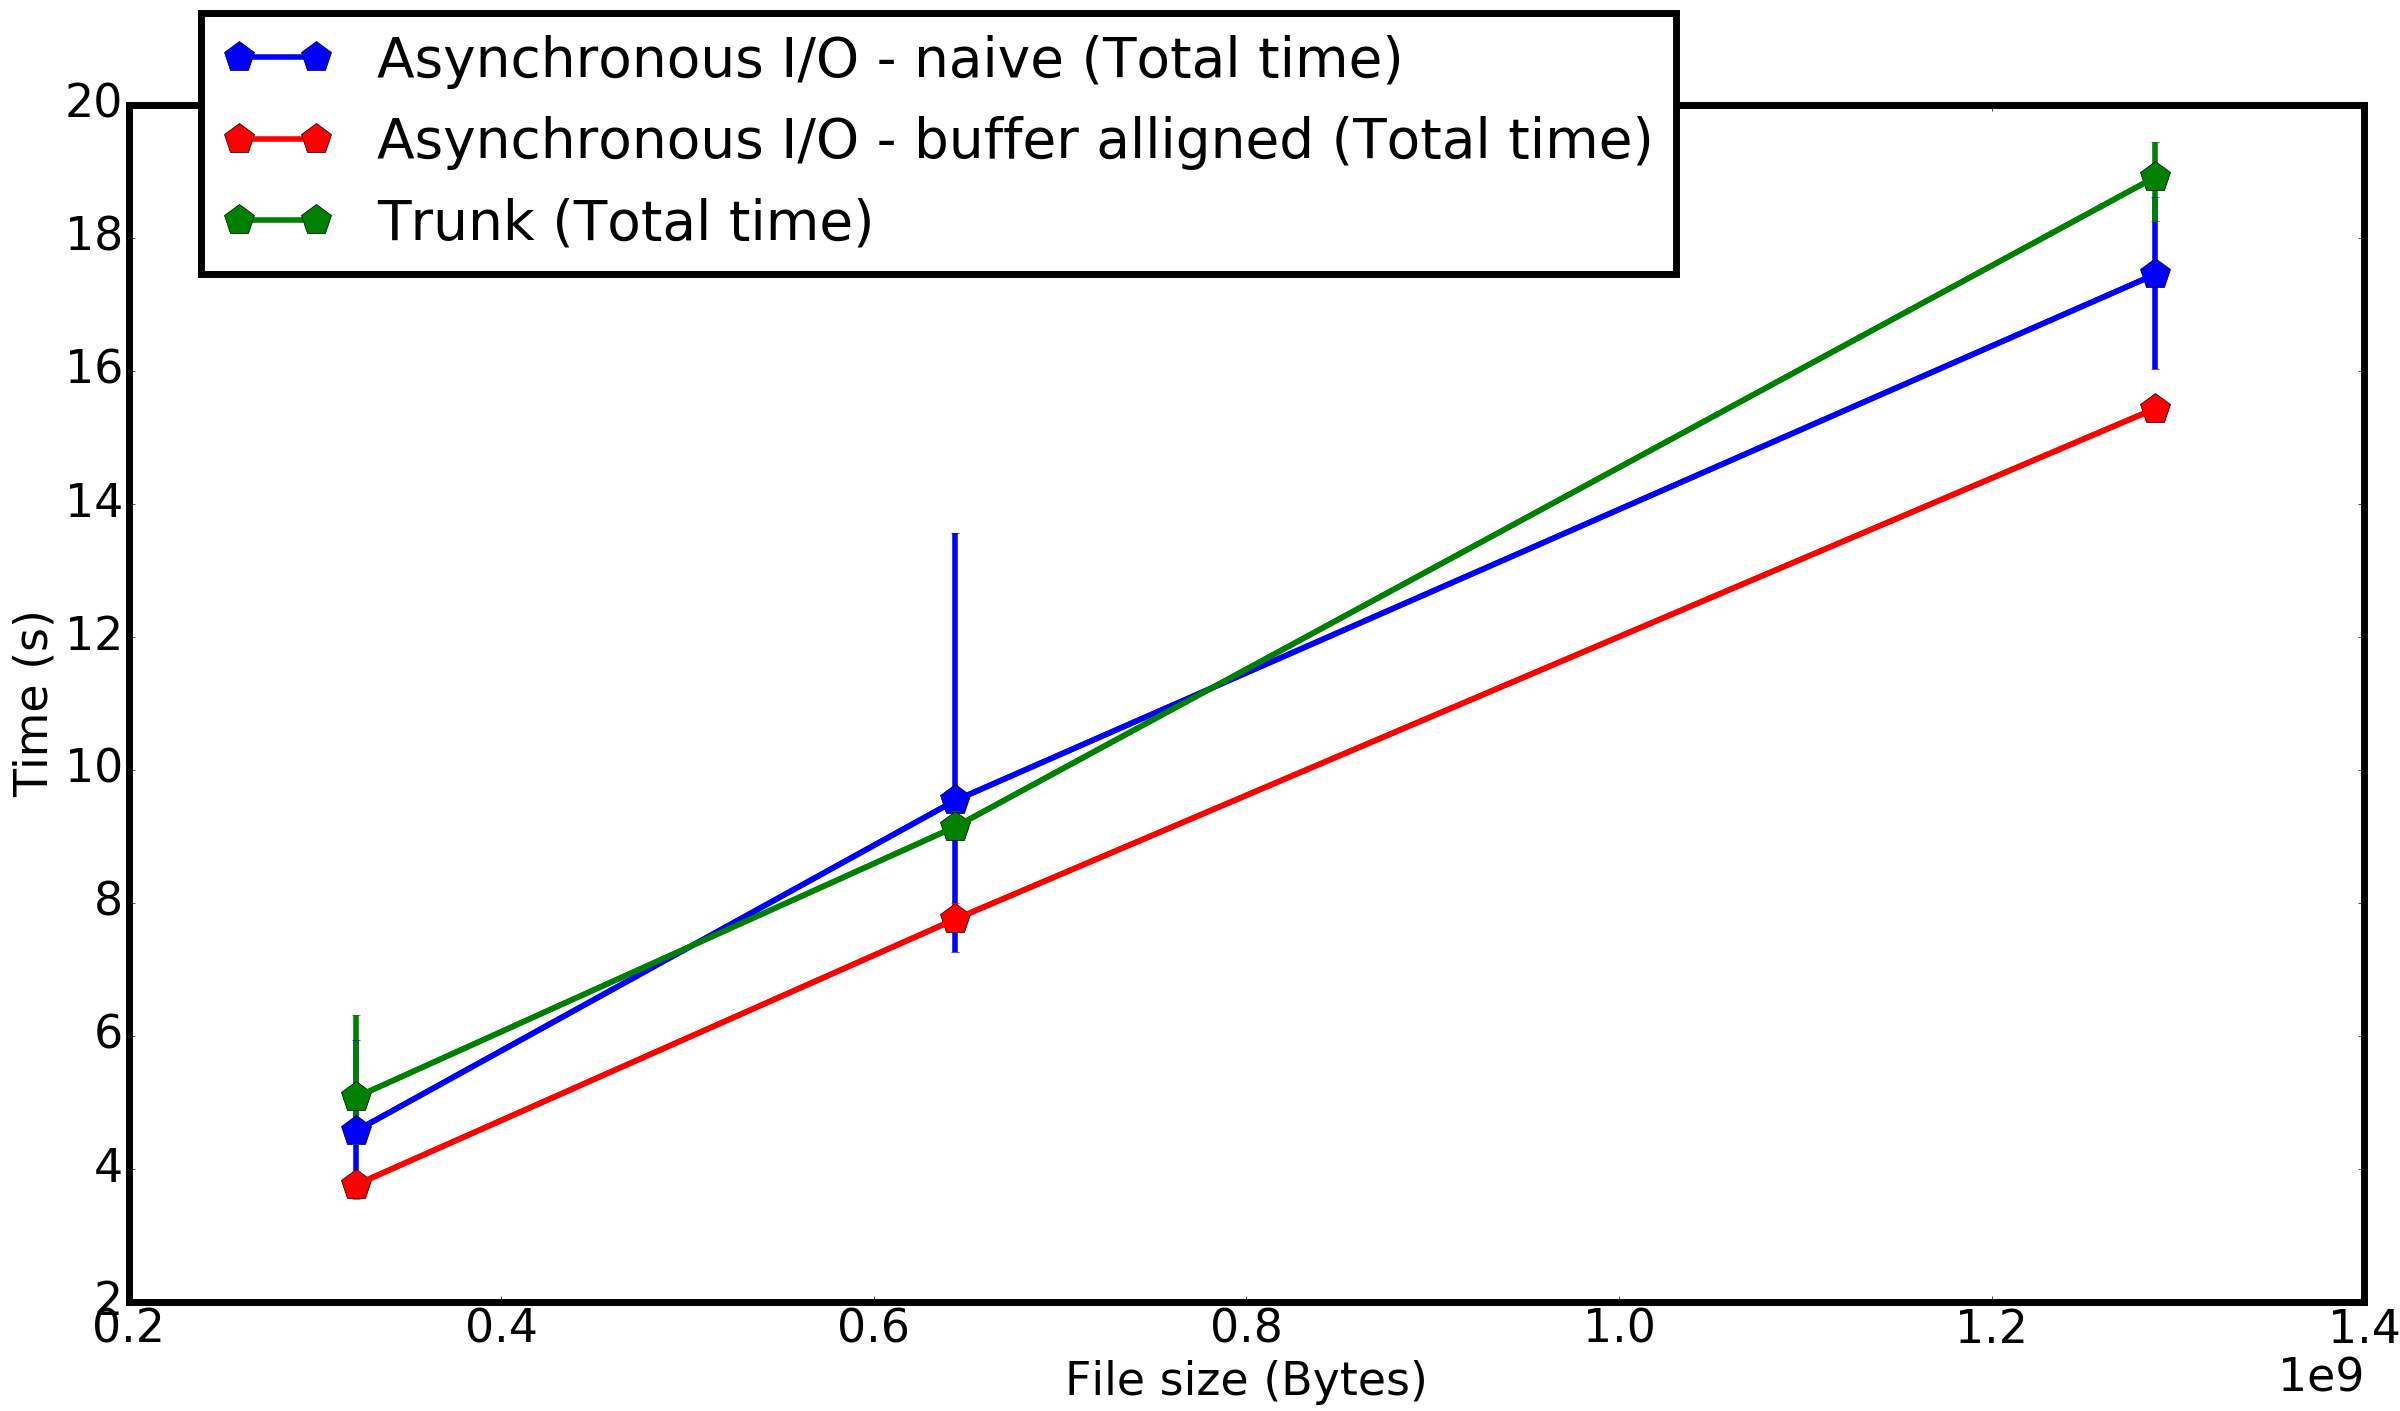
\includegraphics[width=\textwidth]{charts/cubeRemapper_falseSharing_overall_time_hpc.png}
					\caption[]%
					{{\small \targetPlatformHpc \space @ \targetPlatformHpcFrequency}}
					\label{fig:cubeRemapper_falseSharing_overall_time_hpc}
				\end{subfigure}
				\caption{Experimental comparison of the \emph{total} time: proposed \emph{\notationaio}\space (buffer aligned) VS. proposed \emph{\notationaio}\space (naive) VS. \emph{state-of-the-art} (trunk synchronous) implementation of the \toolTargetSoftware.}
				\label{fig:cubeRemapper_falseSharing_overall_time}
			\end{figure*}


	\subsection{Further improvement: adapting the dynamic memory allocation}\label{subsection:customDynamicMemAlloc}
		So far, all the performance gain has been obtained by focusing on the \emph{write} implementation.   Likewise, the improvements described in Sections \ref{subsection:improveSchedulingPolicy} and \ref{subsection:lightenFalseSharing} were aimed at reducing the perturbation of our \emph{write} implementation with respect to the \emph{compute} one.   The objective was to bring the performance of this \emph{compute} implementation \footnote{Unchanged through all the versions of the \toolTargetSoftware that we have presented till now} to the same level as that of the \emph{state-of-the-art} version.\\

		We now assess our full-fledged \notationaio\space implementation of the \toolTargetSoftware.   This final version consists in using the \emph{buffer aligned} version coupled with our custom memory allocator (see Section \ref{subsubsection:customDynamicMemoryAllocation_concept}).   Figure \ref{fig:cubeRemapper_customMemAlloc_overall_time}, which presents the experimental response time, shows that our full-fledged implementation has been able to provide a slight average gain of $19\%$ compared to the \emph{buffer aligned} implementation.   However, much more significant gain ($64\%$) is achieved when compared to the original \emph{state-of-the-art} implementation.

			\begin{figure*}[!h]
				\centering
				\begin{subfigure}[b]{0.475\textwidth}
					\centering
					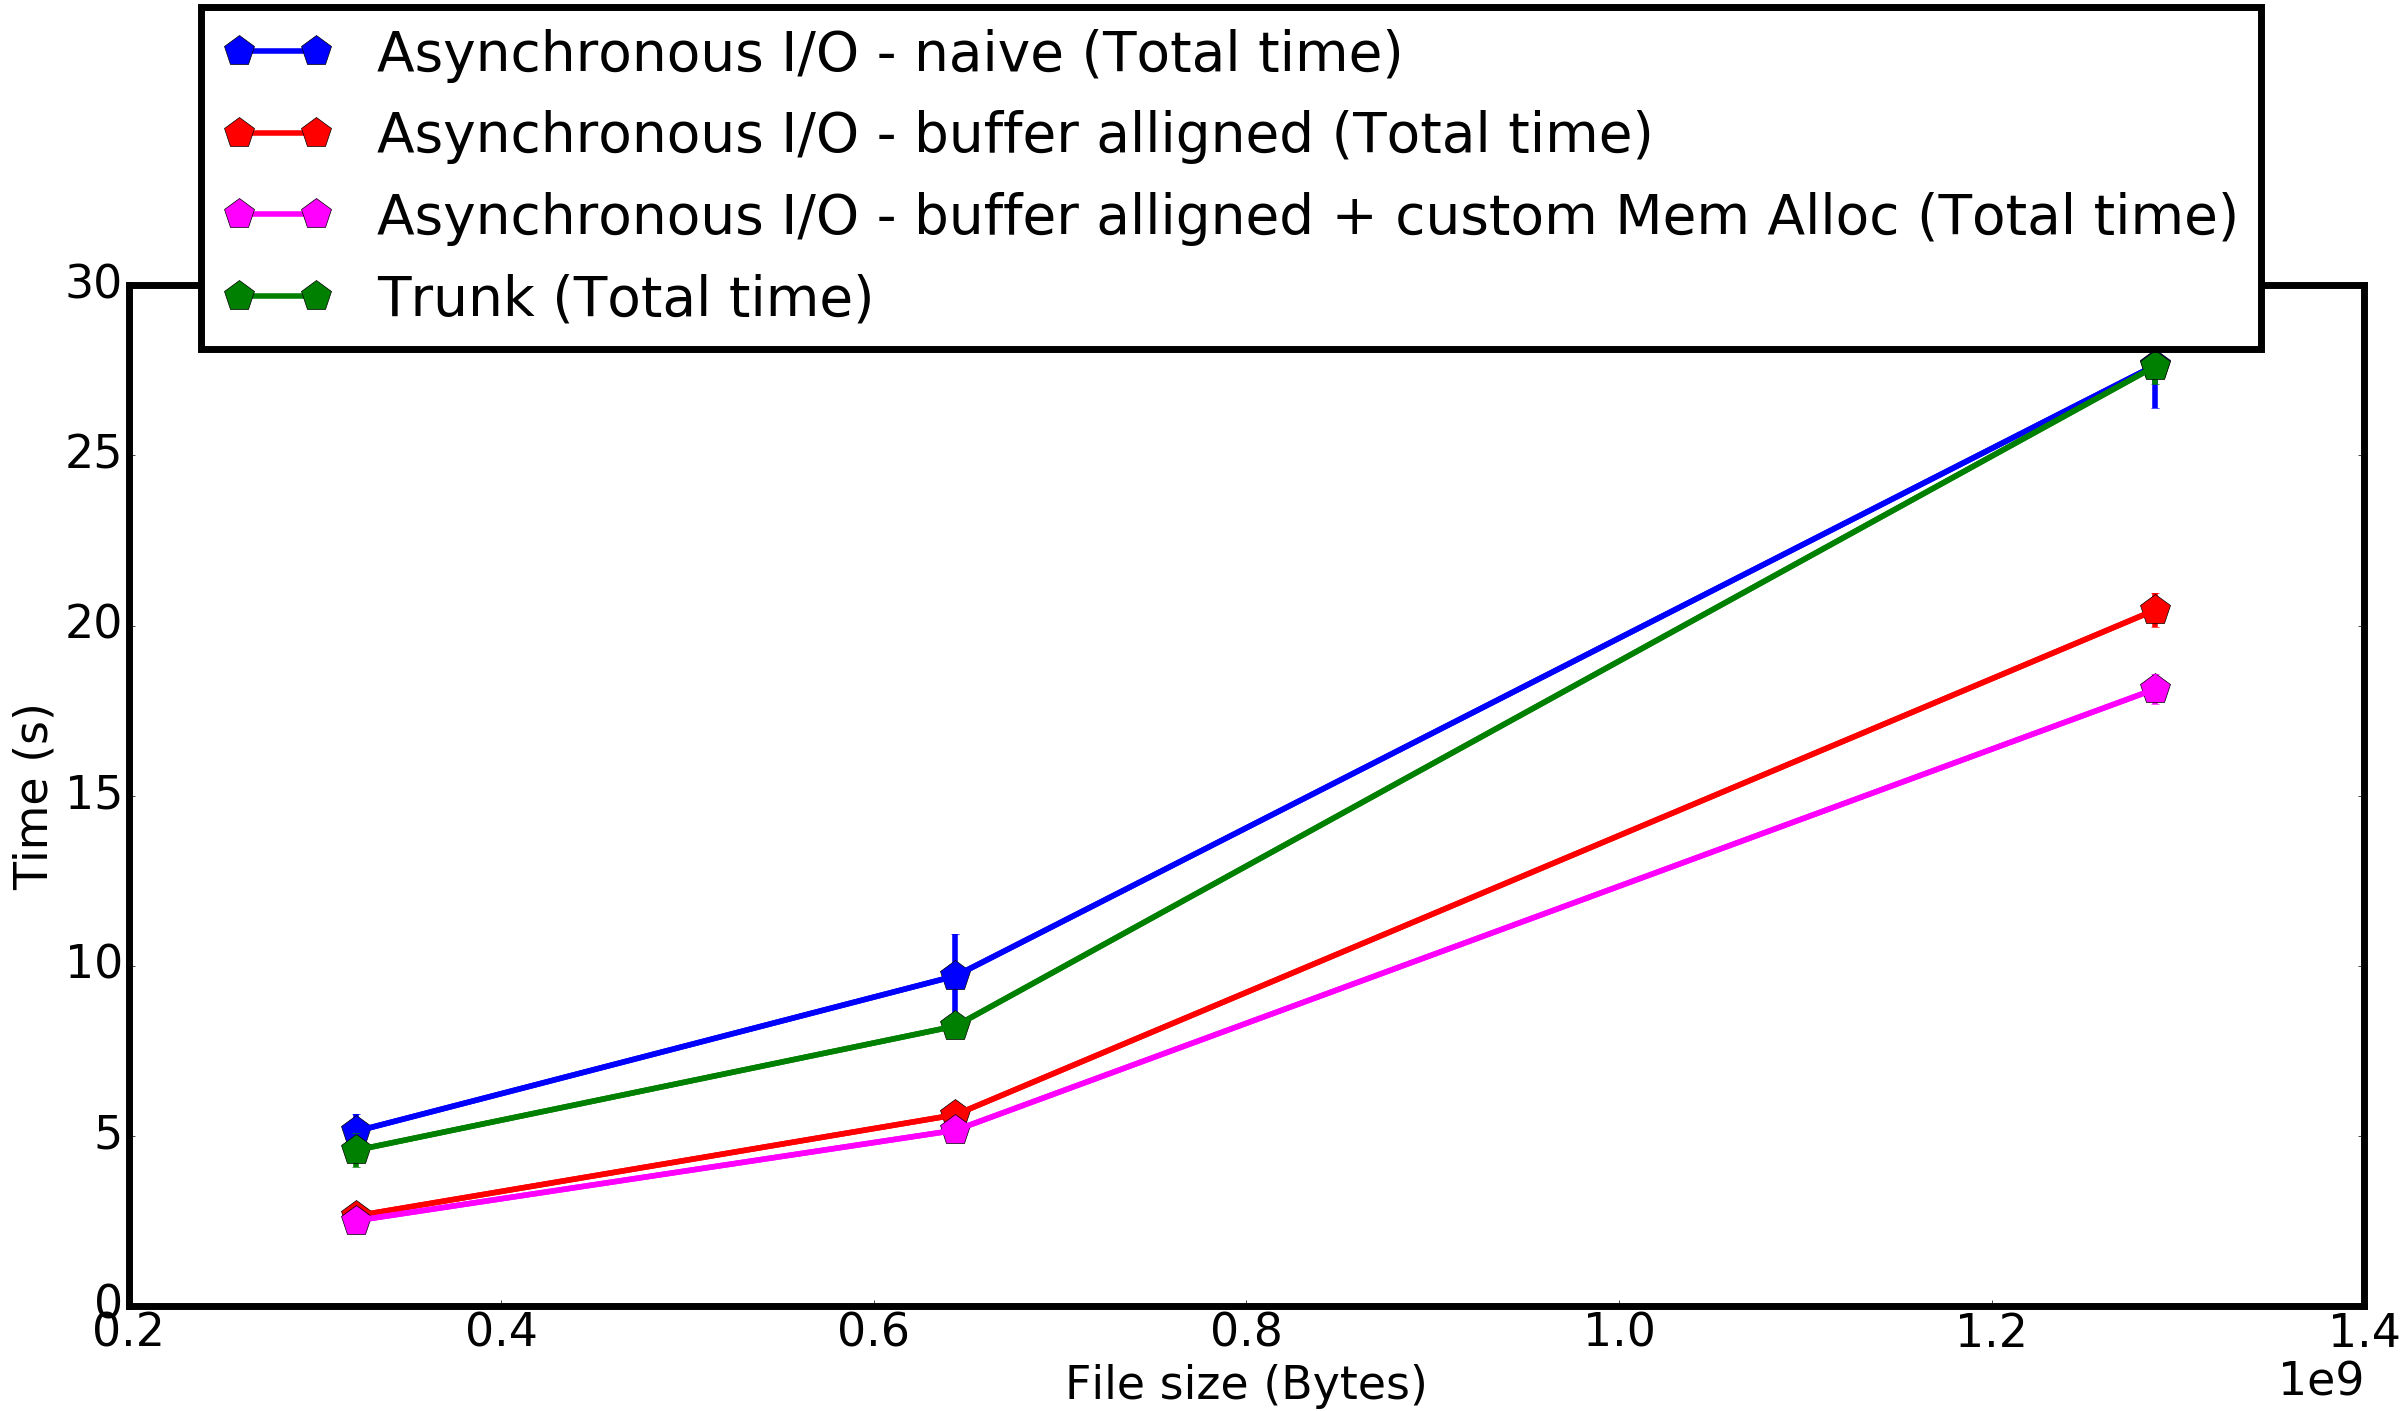
\includegraphics[width=\textwidth]{charts/cubeRemapper_customMemAlloc_overall_time_workstation_8core.png}
					\caption[\targetPlatformLaptop \space @ \targetPlatformLaptopFrequency]%
					{{\small \targetPlatformLaptop \space @ \targetPlatformLaptopFrequency}}
					\label{fig:cubeRemapper_customMemAlloc_overall_time_workstation_8core}
				\end{subfigure}
				\hfill
				\begin{subfigure}[b]{0.475\textwidth}
					\centering
					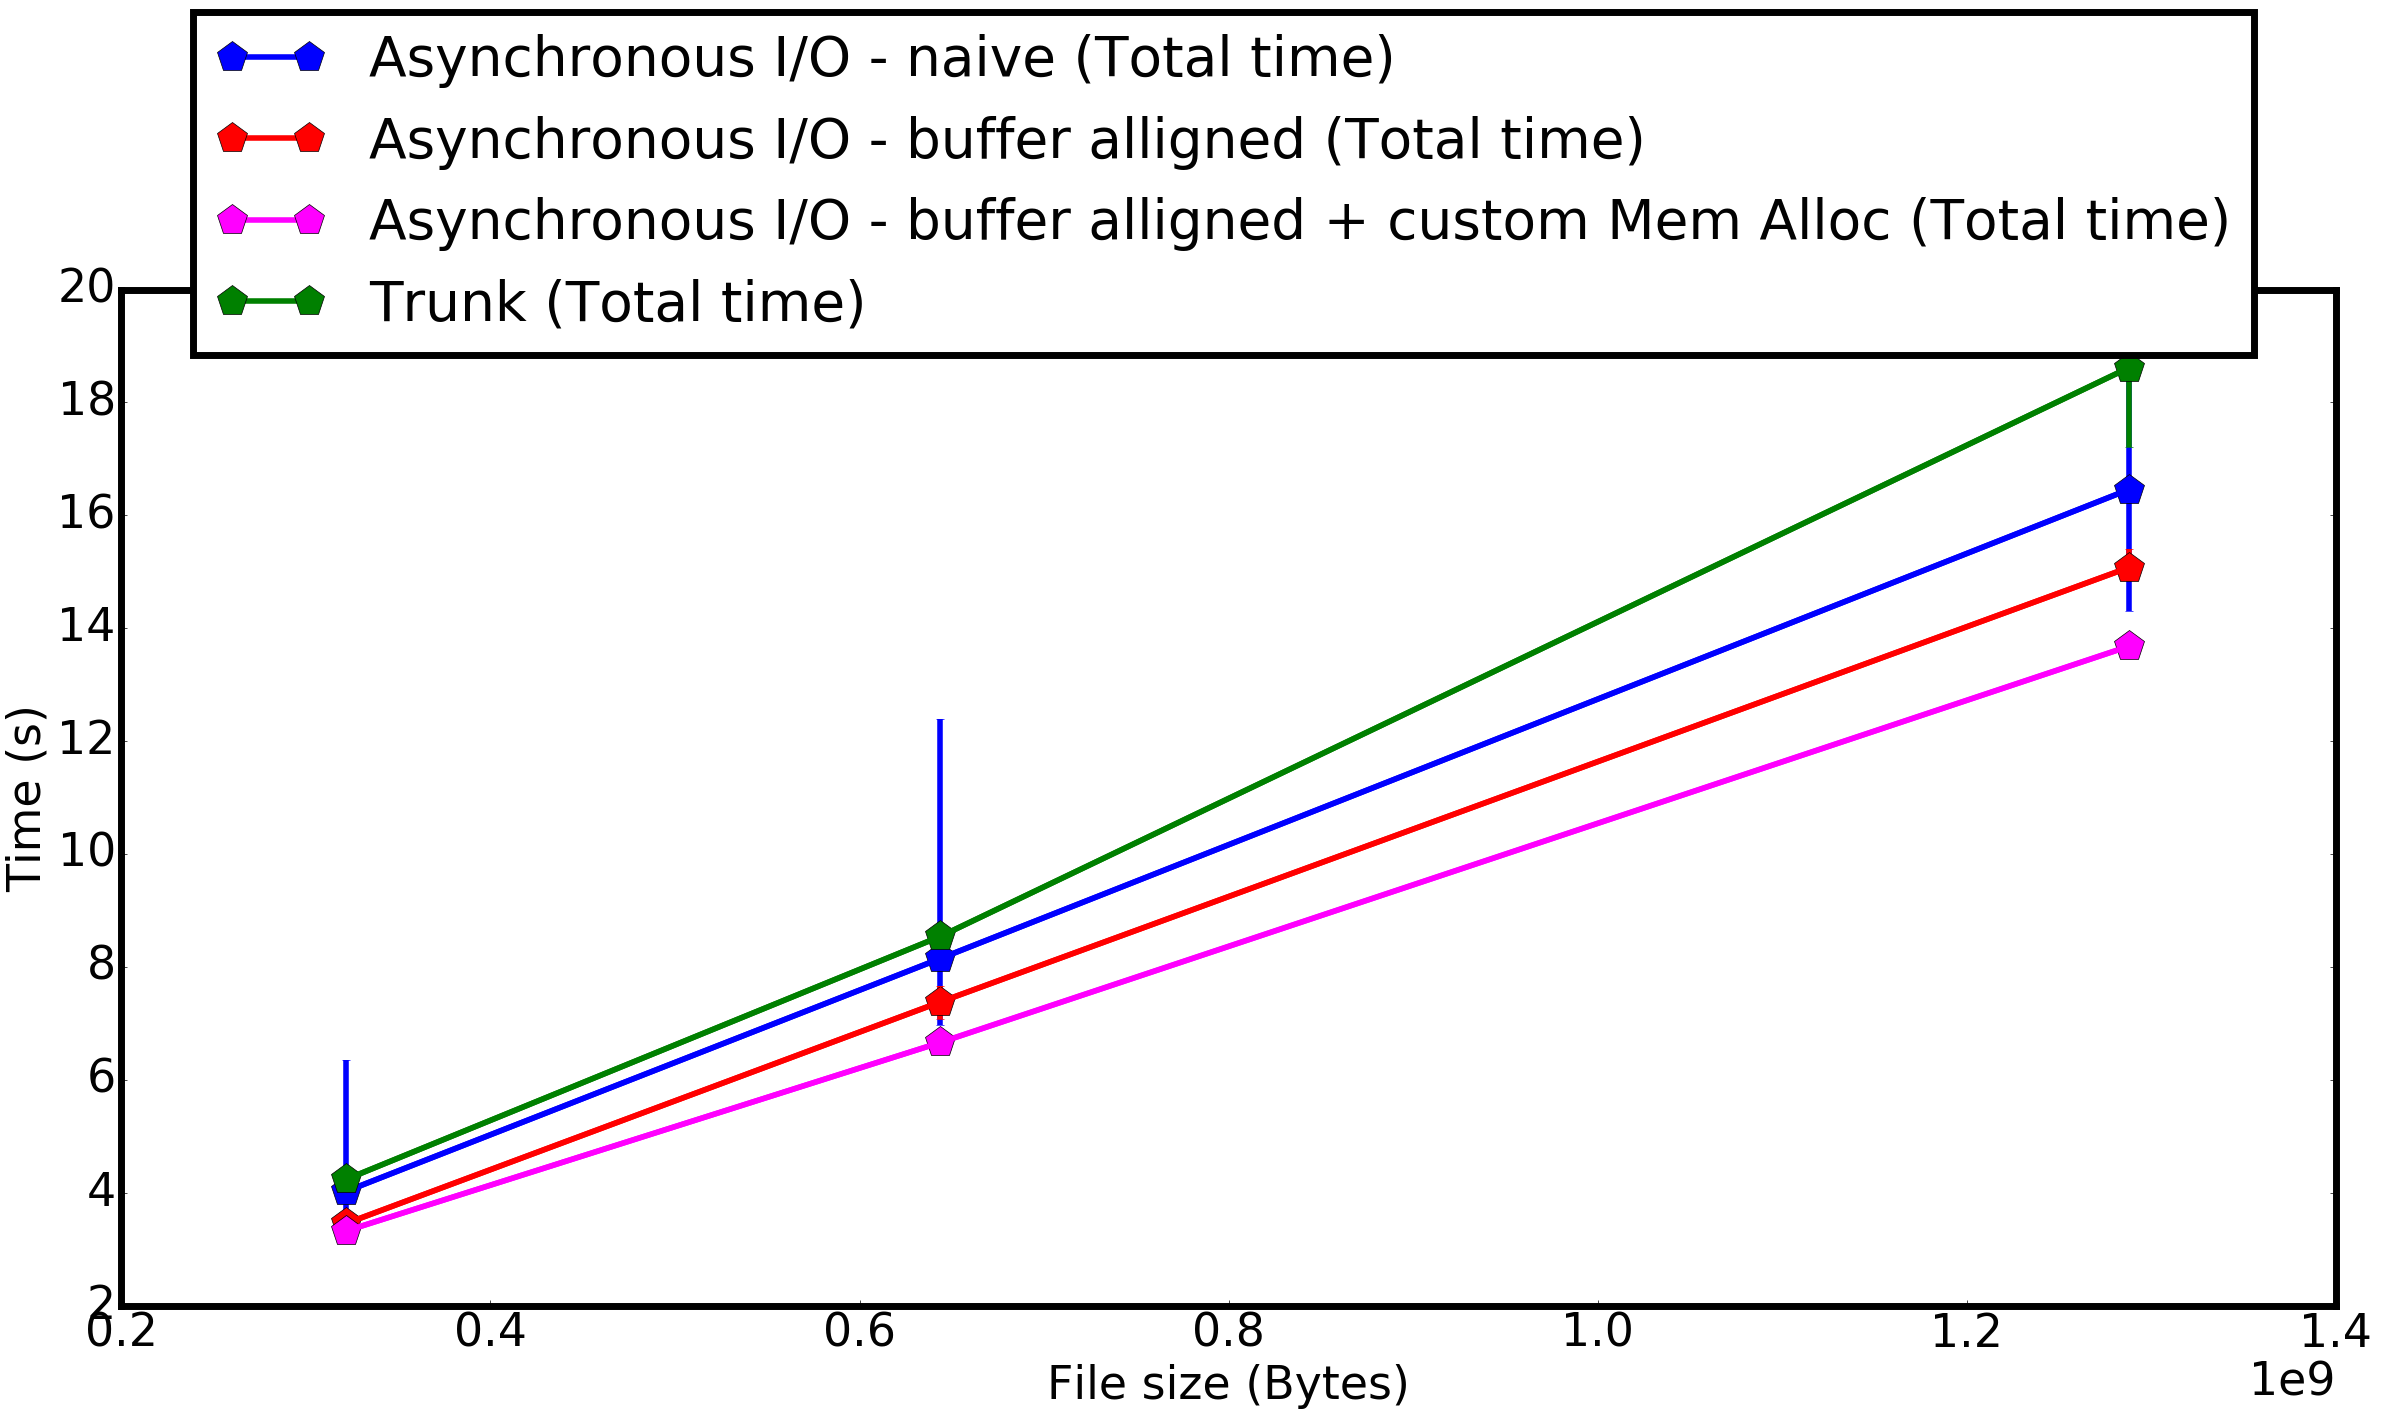
\includegraphics[width=\textwidth]{charts/cubeRemapper_customMemAlloc_overall_time_hpc.png}
					\caption[]%
					{{\small \targetPlatformHpc \space @ \targetPlatformHpcFrequency}}
					\label{fig:cubeRemapper_customMemAlloc_overall_time_hpc}
				\end{subfigure}
				\caption{Experimental comparison of the \emph{total} time: proposed \emph{full-fledged} (buffer aligned + custom mem alloc) VS. proposed \emph{\notationaio}\space (buffer aligned) VS. proposed \emph{\notationaio}\space (naive) VS. \emph{state-of-the-art} (trunk synchronous) implementation of the \toolTargetSoftware.}
				\label{fig:cubeRemapper_customMemAlloc_overall_time}
			\end{figure*}






%This section presents the outcome of the work by interpreting the findings at a higher level of abstraction than the Discussion and by relating these findings to the motivation stated in the Introduction.


%	*******************************
%	********* Simulation results
%	*******************************


\chapter{Conclusion}


	%**************** Context and (objective)
	Performance-profiling and analysing is a mandatory step when developing an HPC-specific application.   In this context, our objective was to outperform a specific tool for HPC-performance analysing: the \toolTargetSoftware.   Given the amount of data (stored on the \notationIO\space disk) to be processed by such a software, our study has focused on enhancing the algorithms of the \notationIO-resource access.\\

	%**************** Finding about the remapper pattern: optimal domain for our solution
	From a theoretical perspective, our study has considered a quite commonly-used computation-pattern\footnote{The pattern followed by the \toolTargetSoftware\space (see Section \ref{section:cubeRemapper_stateOfTheArt})}.   It has proposed an \notationaio\space approach to enhance this pattern as well as the theoretical models related to this custom version of the pattern.   This study has enabled to model accurately the response time of the considered pattern when the \notationIO\space \emph{write} functions are overlapped with the \emph{compute} ones.   Our models also accurately predict the improvement brought by our overlapping approach on a specific implementation of the \toolTargetSoftware\space pattern (referred to as the \emph{\toolSimulationSoftware}).   More importantly, our study has enabled to unveil the parameters that influence most this improvement.\\

	Consequently, our custom implementation of the overlapped \notationIO\space \emph{write}\footnote{Using the POSIX \notationaioShort\space library coupled with our custom synchronization implementation} is shown to potentially outperform the response time of this well-known programming pattern: up to $75\%$ improvement\footnote{Experimental result relative to the considered hardware} compared to the original version of the pattern (assuming an equivalent \emph{compute} and \emph{write} times).\\

	%**************** Finding about the remapper implementation
	From a programmer perspective, our study has highlighted the limitations of using such a well-considered overlapping (\notationaio) approach on the considered pattern (the \toolTargetSoftware\space is used as flagship of this pattern).   This study has made an assessment of some targeted hardware dimensions (processor running/stall time, L3 cache miss-rate) to emphasize the interferences produced by the \notationaio\space approach on the considered pattern.   The study has also proposed two custom solutions\footnote{Namely: adapting the kernel thread-scheduling policy and aligning the dynamic memory allocation with the cache lines} that dramatically soften the impact of such interferences.   Finally, this study has demonstrated the usefulness of our custom memory allocator which was designed to enhance the interaction between the \notationaioComputeThread\space and the \notationaioWriteThreads.\\

	Consequently, our best version of the \toolTargetSoftware\space is shown to bring an improvement up to $64\%$ compared to the original version of this software.\\

	%**************** Perspectives
	In the pattern considered in this study, a buffer created by the \emph{compute} function at a given iteration is never accessed (read nor write) by a later \emph{compute} call.   Thus, this buffer might be written at any more convenient time.   This data-access pattern of the \toolTargetSoftware\space has led us to reduce the overall time-response by overlapping the \notationIO\space access with the \emph{compute} function.   However, it could also be an argument to go further and make the whole pattern of the \toolTargetSoftware\space parallel.   In this context, the \emph{compute} operation could be processed concurrently with the \emph{write} operation as well as with other \emph{compute} calls (at other iterations).   A parallel loop (example: \emph{MPI} or \emph{Cilk} parallel loop) would thus be used in addition to the already overlapped \emph{write} and \emph{compute} thread.




%The main idea we have been following in this paper has been to reduce the overall time by trying to smooth the impact of the first main operation in our pattern: the writing time.\\
%An other approach would be to consider the computation time.   Indeed, each computation is independent from the others.   It is also independent from the write operation.   Thus it could easily and efficiently be scattered on concurrent processor cores (using threads or MPI processes).   A naive analyze of this approach would state that the overall computation time would be divided by the number of concurrently used processors.   But how would the IO devices react to the additional payload (in parallel).   Meanwhile, we saw in (section where we define the model) that the overall behavior of our system depends on the report between the write and the compute time.   So how would this new approach ..... \\

%Obviously, this case has not been considered for lack of time.   But also for some non trivial complexities:   By splitting the compute work on several independent threads (or work-flows)

%=========================================================


%=========================================================
\backmatter


\nocite{*}
%\bibliographystyle{amsplain}
\bibliographystyle{plain} % plain-fr si rapport en français 
\bibliography{bibfile.bib}

%\cleardoublepage % Goes to an odd page
%\pagestyle{empty} % no page number
%~\newpage % goes to a new even page

\end{document}